\title{近十年高考数学三角形三角函数与向量专题汇编}
\author{}
\date{}
\maketitle
\noindent 本汇编按年份排列。每题标题标注原卷、原题号及专题标签；综合题可同时属于多个专题。

\section*{2016 年}

\begin{question}[points=5]
\textbf{来源：}2016 年 全国III卷-理科，第 3 题\quad \textbf{专题：}向量\par
已知向量 $\overrightarrow{BA}=(\frac{1}{2},\frac{\sqrt{3}}{2})$, $\overrightarrow{BC}=(\frac{\sqrt{3}}{2},\frac{1}{2})$, 则 $\angle ABC=$
\begin{choices}
  \item $30^\circ$
  \item $45^\circ$
  \item $60^\circ$
  \item $120^\circ$
\end{choices}
\begin{solution}
\textbf{答案：}$30^\circ$

\textbf{分析：}根据向量 $\overrightarrow{BA},\overrightarrow{BC}$ 的坐标求出 $\overrightarrow{BA}\cdot\overrightarrow{BC},|\overrightarrow{BA}|,|\overrightarrow{BC}|$ 的值, 从而根据向量夹角余弦公式求出 $\cos\angle ABC$, 根据范围得出 $\angle ABC$.

\textbf{详解：}$\overrightarrow{BA}=(\frac{1}{2},\frac{\sqrt{3}}{2}),\overrightarrow{BC}=(\frac{\sqrt{3}}{2},\frac{1}{2})$, $|\overrightarrow{BA}|=1,|\overrightarrow{BC}|=1,\overrightarrow{BA}\cdot\overrightarrow{BC}=\frac{\sqrt{3}}{2}$, $\therefore \cos\angle ABC=\frac{\overrightarrow{BA}\cdot\overrightarrow{BC}}{|\overrightarrow{BA}||\overrightarrow{BC}|}=\frac{\sqrt{3}}{2}$, 又 $0^\circ\le\angle ABC\le180^\circ$, $\therefore\angle ABC=30^\circ$, 故选 A.
\end{solution}
\end{question}

\begin{question}[points=5]
\textbf{来源：}2016 年 全国III卷-理科，第 5 题\quad \textbf{专题：}三角函数\par
若 $\tan\alpha=\frac{3}{4}$, 则 $\cos^2\alpha+2\sin2\alpha=$
\begin{choices}
  \item $\frac{64}{25}$
  \item $\frac{48}{25}$
  \item $1$
  \item $\frac{16}{25}$
\end{choices}
\begin{solution}
\textbf{答案：}$\frac{64}{25}$

\textbf{分析：}将所求的关系式的分母 "$1$" 化为 $(\cos^2\alpha+\sin^2\alpha)$, 再将 "弦" 化 "切" 即可得到答案.

\textbf{详解：}$\because\tan\alpha=\frac{3}{4}$, $\therefore\cos^2\alpha+2\sin2\alpha=\frac{\cos^2\alpha+4\sin\alpha\cos\alpha}{\cos^2\alpha+\sin^2\alpha}=\frac{1+4\tan\alpha}{1+\tan^2\alpha}=\frac{1+3}{1+\frac{9}{16}}=\frac{4}{\frac{25}{16}}=\frac{64}{25}$, 故选 A.
\end{solution}
\end{question}

\begin{question}[points=5]
\textbf{来源：}2016 年 全国III卷-理科，第 8 题\quad \textbf{专题：}三角形、三角函数\par
在 $\triangle ABC$ 中, $B=\frac{\pi}{4}$, $BC$ 边上的高等于 $\frac{1}{3}BC$, 则 $\cos A$ 等于
\begin{choices}
  \item $\frac{3\sqrt{10}}{10}$
  \item $\frac{\sqrt{10}}{10}$
  \item $-\frac{\sqrt{10}}{10}$
  \item $-\frac{3\sqrt{10}}{10}$
\end{choices}
\begin{solution}
\textbf{答案：}$-\frac{\sqrt{10}}{10}$

\textbf{分析：}作出图形, 令 $\angle DAC=\theta$, 利用两角和的余弦求 $\cos A$.

\textbf{详解：}设 $\triangle ABC$ 中角 $A,B,C$ 对应的边分别为 $a,b,c$, $AD\perp BC$ 于 $D$, 令 $\angle DAC=\theta$. $\because B=\frac{\pi}{4}, BC$ 边上的高 $AD=h=\frac{1}{3}BC=\frac{a}{3}$, $\therefore BD=AD=\frac{a}{3}, CD=\frac{2a}{3}$. 在 $\mathrm{Rt}\triangle ADC$ 中, $\cos\theta=\frac{AD}{AC}=\frac{\frac{a}{3}}{\sqrt{(\frac{a}{3})^2+(\frac{2a}{3})^2}}=\frac{\sqrt{5}}{5}$, 故 $\sin\theta=\frac{2\sqrt{5}}{5}$, $\therefore \cos A=\cos(\frac{\pi}{4}+\theta)=\cos\frac{\pi}{4}\cos\theta-\sin\frac{\pi}{4}\sin\theta=\frac{\sqrt{2}}{2}\cdot\frac{\sqrt{5}}{5}-\frac{\sqrt{2}}{2}\cdot\frac{2\sqrt{5}}{5}=-\frac{\sqrt{10}}{10}$, 故选 C.
\end{solution}
\end{question}

\begin{question}[points=5]
\textbf{来源：}2016 年 全国III卷-理科，第 14 题\quad \textbf{专题：}三角函数\par
函数 $y=\sin x-\sqrt{3}\cos x$ 的图象可由函数 $y=\sin x+\sqrt{3}\cos x$ 的图象至少向右平移  个单位长度得到.
\fillin[{$\frac{2\pi}{3}$}]
\begin{solution}
\textbf{答案：}$\frac{2\pi}{3}$

\textbf{分析：}令 $f(x)=\sin x+\sqrt{3}\cos x=2\sin(x+\frac{\pi}{3})$, 则 $f(x-\phi)=2\sin(x+\frac{\pi}{3}-\phi)$, 依题意可得 $2\sin(x+\frac{\pi}{3}-\phi)=2\sin(x-\frac{\pi}{3})$, 由 $\frac{\pi}{3}-\phi=2k\pi-\frac{\pi}{3}$ 可得答案.

\textbf{详解：}$y=f(x)=\sin x+\sqrt{3}\cos x=2\sin(x+\frac{\pi}{3})$, $y=\sin x-\sqrt{3}\cos x=2\sin(x-\frac{\pi}{3})$. $f(x-\phi)=2\sin(x+\frac{\pi}{3}-\phi)$ ($\phi>0$), 令 $2\sin(x+\frac{\pi}{3}-\phi)=2\sin(x-\frac{\pi}{3})$, 则 $\frac{\pi}{3}-\phi=2k\pi-\frac{\pi}{3}$, 即 $\phi=\frac{2\pi}{3}-2k\pi$, 当 $k=0$ 时, 正数 $\phi_{\min}=\frac{2\pi}{3}$. 故答案为 $\frac{2\pi}{3}$.
\end{solution}
\end{question}

\begin{question}[points=12]
\textbf{来源：}2016 年 全国III卷-理科，第 21 题\quad \textbf{专题：}三角函数\par
设函数 $f(x)=a\cos2x+(a-1)(\cos x+1)$, 其中 $a>0$, 记 $|f(x)|$ 的最大值为 $A$.

(Ⅰ) 求 $f'(x)$;

(Ⅱ) 求 $A$;

(Ⅲ) 证明: $|f'(x)|\le2A$.
\begin{solution}

\textbf{分析：}(Ⅰ) 根据复合函数的导数公式进行求解. (Ⅱ) 讨论 $a$ 的取值, 利用分类讨论的思想方法, 结合换元法以及一元二次函数的最值的性质进行求解. (Ⅲ) 结合绝对值不等式的性质即可证明.

\textbf{详解：}(Ⅰ) 解: $f'(x)=-2a\sin2x-(a-1)\sin x$.
(Ⅱ) 当 $a\ge1$ 时, $|f(x)|=|a\cos2x+(a-1)(\cos x+1)|\le a|\cos2x|+(a-1)|\cos x+1|\le a|\cos2x|+(a-1)(|\cos x|+1)\le a+2(a-1)=3a-2=f(0)$, 因此 $A=3a-2$. 当 $0<a<1$ 时, $f(x)=a\cos2x+(a-1)(\cos x+1)=2a\cos^2x+(a-1)\cos x-1$, 令 $g(t)=2at^2+(a-1)t-1$, 则 $A$ 是 $|g(t)|$ 在 $[-1,1]$ 上的最大值, $g(-1)=a$, $g(1)=3a-2$, 且当 $t=\frac{1-a}{4a}$ 时, $g(t)$ 取得极小值 $g(\frac{1-a}{4a})=-\frac{(a-1)^2}{8a}-1=-\frac{(a-1)^2+8a}{8a}=-\frac{a^2+6a+1}{8a}$. 令 $-1<\frac{1-a}{4a}<1$, 得 $a>\frac{1}{5}$. ①当 $0<a\le\frac{1}{5}$ 时, $g(t)$ 在 $(-1,1)$ 内无极值点, $|g(-1)|=a$, $|g(1)|=2-3a$, $|g(-1)|<|g(1)|$, $\therefore A=2-3a$; ②当 $\frac{1}{5}<a<1$ 时, 由 $g(-1)-g(1)=2(1-a)>0$, 得 $g(-1)>g(1)>g(\frac{1-a}{4a})$, 又 $|g(\frac{1-a}{4a})|-|g(-1)|=\frac{(1-a)^2}{8a}-\frac{(1-a)^2}{8a}?$ 实际上 $|g(\frac{1-a}{4a})|=\frac{a^2+6a+1}{8a}$, $|g(-1)|=a$, $\frac{a^2+6a+1}{8a}-a=\frac{a^2+6a+1-8a^2}{8a}=\frac{-7a^2+6a+1}{8a}=\frac{-(7a+1)(a-1)}{8a}>0$, $\therefore A=|g(\frac{1-a}{4a})|=\frac{a^2+6a+1}{8a}$. 综上, $A=\begin{cases}2-3a, &0<a\le\frac{1}{5}\\ \frac{a^2+6a+1}{8a}, &\frac{1}{5}<a<1\\ 3a-2, &a\ge1\end{cases}$.
(Ⅲ) 证明: 由(Ⅰ)可得 $|f'(x)|=|-2a\sin2x-(a-1)\sin x|\le2a+|a-1|$. 当 $0<a\le\frac{1}{5}$ 时, $|f'(x)|<1+a\le2-4a<2(2-3a)=2A$; 当 $\frac{1}{5}<a<1$ 时, $A=\frac{a^2+6a+1}{8a}=\frac{a}{8}+\frac{3}{4}+\frac{1}{8a}>1$, $\therefore|f'(x)|\le1+a\le2A$; 当 $a\ge1$ 时, $|f'(x)|\le3a-1\le6a-4=2A$. 综上, $|f'(x)|\le2A$.
\end{solution}
\end{question}

\begin{question}[points=5]
\textbf{来源：}2016 年 全国III卷-文科，第 3 题\quad \textbf{专题：}向量\par
已知向量 $\overrightarrow{BA}=(\dfrac{1}{2},\dfrac{\sqrt{3}}{2})$, $\overrightarrow{BC}=(\dfrac{\sqrt{3}}{2},\dfrac{1}{2})$, 则 $\angle ABC=$ ( )
\begin{choices}
  \item $30^{\circ}$
  \item $45^{\circ}$
  \item $60^{\circ}$
  \item $120^{\circ}$
\end{choices}
\begin{solution}
\textbf{答案：}$30^{\circ}$

\textbf{分析：}根据向量 $\overrightarrow{BA}$ 和 $\overrightarrow{BC}$ 的坐标求出 $\overrightarrow{BA}\cdot\overrightarrow{BC}$ 及 $|\overrightarrow{BA}|,|\overrightarrow{BC}|$ 的值, 从而根据向量夹角余弦公式即可求出 $\cos\angle ABC$ 的值, 根据 $\angle ABC$ 的范围便可得出 $\angle ABC$ 的值.

\textbf{详解：}$\overrightarrow{BA}=(\dfrac{1}{2},\dfrac{\sqrt{3}}{2})$, $\overrightarrow{BC}=(\dfrac{\sqrt{3}}{2},\dfrac{1}{2})$; 则 $\overrightarrow{BA}\cdot\overrightarrow{BC}=\dfrac{1}{2}\cdot\dfrac{\sqrt{3}}{2}+\dfrac{\sqrt{3}}{2}\cdot\dfrac{1}{2}=\dfrac{\sqrt{3}}{2}$, $|\overrightarrow{BA}|=1$, $|\overrightarrow{BC}|=1$; 所以 $\cos\angle ABC=\dfrac{\overrightarrow{BA}\cdot\overrightarrow{BC}}{|\overrightarrow{BA}||\overrightarrow{BC}|}=\dfrac{\sqrt{3}}{2}$; 又 $0^{\circ}\le\angle ABC\le180^{\circ}$; 所以 $\angle ABC=30^{\circ}$. 故选 A.
\end{solution}
\end{question}

\begin{question}[points=5]
\textbf{来源：}2016 年 全国III卷-文科，第 6 题\quad \textbf{专题：}三角函数\par
若 $\tan\theta=\dfrac{1}{3}$, 则 $\cos2\theta=$ ( )
\begin{choices}
  \item $\dfrac{4}{5}$
  \item $\dfrac{1}{5}$
  \item $\dfrac{1}{5}$
  \item $\dfrac{3}{5}$
\end{choices}
\begin{solution}
\textbf{答案：}$\dfrac{4}{5}$

\textbf{分析：}原式利用二倍角的余弦函数公式变形, 再利用同角三角函数间的基本关系化简, 将 $\tan\theta$ 的值代入计算即可求出值.

\textbf{详解：}$\tan\theta=\dfrac{1}{3}$, 则 $\cos2\theta=2\cos^2\theta-1=\dfrac{2}{1+\tan^2\theta}-1=\dfrac{2}{1+\frac{1}{9}}-1=\dfrac{2}{\frac{10}{9}}-1=\dfrac{18}{10}-1=\dfrac{8}{10}=\dfrac{4}{5}$. 故选 D.
\end{solution}
\end{question}

\begin{question}[points=5]
\textbf{来源：}2016 年 全国III卷-文科，第 9 题\quad \textbf{专题：}三角形、三角函数\par
在 $\triangle ABC$ 中, $B=\dfrac{\pi}{4}$, $BC$ 边上的高等于 $\dfrac{1}{3}BC$, 则 $\sin A=$ ( )
\begin{choices}
  \item $\dfrac{3}{10}$
  \item $\dfrac{\sqrt{10}}{10}$
  \item $\dfrac{\sqrt{5}}{5}$
  \item $\dfrac{3\sqrt{10}}{10}$
\end{choices}
\begin{solution}
\textbf{答案：}$\dfrac{3\sqrt{10}}{10}$

\textbf{分析：}由已知, 结合勾股定理和余弦定理, 求出 $AB$, $AC$, 再由三角形面积公式, 可得 $\sin A$.

\textbf{详解：}在 $\triangle ABC$ 中, $B=\dfrac{\pi}{4}$, $BC$ 边上的高等于 $\dfrac{1}{3}BC$, 所以 $AB=\dfrac{\sqrt{2}}{3}BC$. 由余弦定理 $AC^2=AB^2+BC^2-2\cdot AB\cdot BC\cdot\cos B=\dfrac{2}{9}BC^2+BC^2-2\cdot\dfrac{\sqrt{2}}{3}BC\cdot BC\cdot\dfrac{\sqrt{2}}{2}=\dfrac{2}{9}BC^2+BC^2-\dfrac{2}{3}BC^2=\dfrac{5}{9}BC^2$, 故 $AC=\dfrac{\sqrt{5}}{3}BC$. 由面积公式 $\dfrac{1}{2}\cdot BC\cdot\dfrac{1}{3}BC=\dfrac{1}{2}\cdot AB\cdot AC\cdot\sin A$, 即 $\dfrac{1}{6}BC^2=\dfrac{1}{2}\cdot\dfrac{\sqrt{2}}{3}BC\cdot\dfrac{\sqrt{5}}{3}BC\cdot\sin A$, 解得 $\sin A=\dfrac{3\sqrt{10}}{10}$. 故选 D.
\end{solution}
\end{question}

\begin{question}[points=5]
\textbf{来源：}2016 年 全国III卷-文科，第 14 题\quad \textbf{专题：}三角函数\par
函数 $y=\sin x-\sqrt{3}\cos x$ 的图象可由函数 $y=2\sin x$ 的图象至少向右平移  个单位长度得到.
\fillin[{$\dfrac{\pi}{3}$}]
\begin{solution}
\textbf{答案：}$\dfrac{\pi}{3}$

\textbf{分析：}令 $f(x)=2\sin x$, 则 $f(x-\varphi)=2\sin(x-\varphi)$, 依题意可得 $2\sin(x-\varphi)=2\sin(x-\frac{\pi}{3})$, 由 $-\varphi=2k\pi-\frac{\pi}{3}$ $(k\in\mathbb{Z})$, 可得答案.

\textbf{详解：}$y=\sin x-\sqrt{3}\cos x=2\sin(x-\frac{\pi}{3})$. 令 $f(x)=2\sin x$, 则 $f(x-\varphi)=2\sin(x-\varphi)$ $(\varphi>0)$. 依题意 $2\sin(x-\varphi)=2\sin(x-\frac{\pi}{3})$, 故 $-\varphi=2k\pi-\frac{\pi}{3}$ $(k\in\mathbb{Z})$, 即 $\varphi=-2k\pi+\frac{\pi}{3}$ $(k\in\mathbb{Z})$. 当 $k=0$ 时, 正数 $\varphi_{\min}=\dfrac{\pi}{3}$. 故答案为 $\dfrac{\pi}{3}$.
\end{solution}
\end{question}

\begin{question}[points=5]
\textbf{来源：}2016 年 全国II卷-理科，第 3 题\quad \textbf{专题：}向量\par
已知向量$\overrightarrow{a}=(1,m)$，$\overrightarrow{b}=(3,-2)$，且$(\overrightarrow{a}+\overrightarrow{b})\perp\overrightarrow{b}$，则$m=$（\quad）
\begin{choices}
  \item $-8$
  \item $-6$
  \item $6$
  \item $8$
\end{choices}
\begin{solution}
\textbf{答案：}$8$

\textbf{分析：}求出向量$\overrightarrow{a}+\overrightarrow{b}$的坐标，根据向量垂直的充要条件，构造关于$m$的方程，解得答案．

\textbf{详解：}$\overrightarrow{a}+\overrightarrow{b}=(4,m-2)$，由$(\overrightarrow{a}+\overrightarrow{b})\perp\overrightarrow{b}$得$4\times3+(m-2)\times(-2)=0$，解得$m=8$．故选D．
\end{solution}
\end{question}

\begin{question}[points=5]
\textbf{来源：}2016 年 全国II卷-理科，第 7 题\quad \textbf{专题：}三角函数\par
若将函数$y=2\sin2x$的图象向左平移$\frac{\pi}{12}$个单位长度，则平移后的图象的对称轴为（\quad）
\begin{choices}
  \item $x=\frac{k\pi}{2}-\frac{\pi}{6}\ (k\in\mathbb{Z})$
  \item $x=\frac{k\pi}{2}+\frac{\pi}{6}\ (k\in\mathbb{Z})$
  \item $x=\frac{k\pi}{2}-\frac{\pi}{12}\ (k\in\mathbb{Z})$
  \item $x=\frac{k\pi}{2}+\frac{\pi}{12}\ (k\in\mathbb{Z})$
\end{choices}
\begin{solution}
\textbf{答案：}$x=\frac{k\pi}{2}+\frac{\pi}{6}\ (k\in\mathbb{Z})$

\textbf{分析：}利用函数$y=A\sin(\omega x+\varphi)$的图象的变换及正弦函数的对称性可得答案．

\textbf{详解：}平移后得$y=2\sin\left[2\left(x+\frac{\pi}{12}\right)\right]=2\sin\left(2x+\frac{\pi}{6}\right)$，令$2x+\frac{\pi}{6}=k\pi+\frac{\pi}{2}$，得$x=\frac{k\pi}{2}+\frac{\pi}{6}$．故选B．
\end{solution}
\end{question}

\begin{question}[points=5]
\textbf{来源：}2016 年 全国II卷-理科，第 9 题\quad \textbf{专题：}三角函数\par
若$\cos\left(\frac{\pi}{4}-\alpha\right)=\frac{3}{5}$，则$\sin2\alpha=$（\quad）
\begin{choices}
  \item $\frac{7}{25}$
  \item $\frac{1}{5}$
  \item $-\frac{1}{5}$
  \item $-\frac{7}{25}$
\end{choices}
\begin{solution}
\textbf{答案：}$-\frac{7}{25}$

\textbf{分析：}法1：利用诱导公式化$\sin2\alpha=\cos\left(\frac{\pi}{2}-2\alpha\right)$，再利用二倍角的余弦可得答案．法2：利用余弦二倍角公式将左边展开，可以得$\sin\alpha+\cos\alpha$的值，再平方，即得$\sin2\alpha$的值．

\textbf{详解：}法1：$\sin2\alpha=\cos\left(\frac{\pi}{2}-2\alpha\right)=\cos\left[2\left(\frac{\pi}{4}-\alpha\right)\right]=2\cos^2\left(\frac{\pi}{4}-\alpha\right)-1=2\times\frac{9}{25}-1=-\frac{7}{25}$．故选D．
\end{solution}
\end{question}

\begin{question}[points=5]
\textbf{来源：}2016 年 全国II卷-理科，第 11 题\quad \textbf{专题：}三角函数\par
已知$F_1$，$F_2$是双曲线$E:\frac{x^2}{a^2}-\frac{y^2}{b^2}=1$的左，右焦点，点$M$在$E$上，$MF_1$与$x$轴垂直，$\sin\angle MF_2F_1=\frac{1}{3}$，则$E$的离心率为（\quad）
\begin{choices}
  \item $\sqrt{2}$
  \item $\frac{3}{2}$
  \item $\sqrt{3}$
  \item $2$
\end{choices}
\begin{solution}
\textbf{答案：}$\sqrt{2}$

\textbf{分析：}由条件$MF_1\perp x$轴，$\sin\angle MF_2F_1=\frac13$，列出关系式，从而可求离心率．

\textbf{详解：}设$|MF_1|=m$，则$|MF_2|=2a+m$，在直角三角形中$\sin\angle MF_2F_1=\frac{m}{2a+m}=\frac13$，解得$m=a$，又$m=\frac{b^2}{a}$，故$\frac{b^2}{a}=a$，即$b^2=a^2$，$c^2=2a^2$，$e=\sqrt{2}$．故选A．
\end{solution}
\end{question}

\begin{question}[points=5]
\textbf{来源：}2016 年 全国II卷-理科，第 13 题\quad \textbf{专题：}三角形、三角函数\par
$\triangle ABC$的内角$A$，$B$，$C$的对边分别为$a$，$b$，$c$，若$\cos A=\frac{4}{5}$，$\cos C=\frac{5}{13}$，$a=1$，则$b=$．
\fillin[{$\frac{21}{13}$}]
\begin{solution}
\textbf{答案：}$\frac{21}{13}$

\textbf{分析：}运用同角的平方关系可得$\sin A$，$\sin C$，再由诱导公式和两角和的正弦公式，可得$\sin B$，运用正弦定理可得$b=\frac{a\sin B}{\sin A}$，代入计算即可得到所求值．

\textbf{详解：}$\sin A=\frac{3}{5}$，$\sin C=\frac{12}{13}$，$\sin B=\sin(A+C)=\frac{3}{5}\times\frac{5}{13}+\frac{4}{5}\times\frac{12}{13}=\frac{63}{65}$，由正弦定理$b=\frac{a\sin B}{\sin A}=\frac{1\times\frac{63}{65}}{\frac{3}{5}}=\frac{21}{13}$．
\end{solution}
\end{question}

\begin{question}[points=5]
\textbf{来源：}2016 年 全国II卷-文科，第 3 题\quad \textbf{专题：}三角函数\par
函数$y=A\sin(\omega x+\varphi)$的部分图象如图所示，则

\begin{center}
  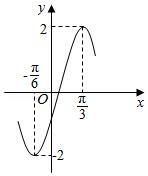
\includegraphics[width=.42\linewidth]{assets/asset-015-01.jpg}
\end{center}
\begin{choices}
  \item $y=2\sin(2x-\frac{\pi}{6})$
  \item $y=2\sin(2x-\frac{\pi}{3})$
  \item $y=2\sin(x+\frac{\pi}{6})$
  \item $y=2\sin(x+\frac{\pi}{3})$
\end{choices}
\begin{solution}
\textbf{答案：}$y=2\sin(2x-\frac{\pi}{6})$

\textbf{分析：}由图得$A=2$，$\frac{T}{4}=\frac{\pi}{4}$，故$T=\pi$，$\omega=2$，代入点$(\frac{\pi}{12},2)$得$\varphi=-\frac{\pi}{6}$。
\end{solution}
\end{question}

\begin{question}[points=5]
\textbf{来源：}2016 年 全国II卷-文科，第 11 题\quad \textbf{专题：}三角函数\par
函数$f(x)=\cos2x+6\cos(\frac{\pi}{2}-x)$的最大值为
\begin{choices}
  \item $4$
  \item $5$
  \item $6$
  \item $7$
\end{choices}
\begin{solution}
\textbf{答案：}$5$

\textbf{分析：}$f(x)=1-2\sin^2x+6\sin x$，令$t=\sin x\in[-1,1]$，$y=-2t^2+6t+1$，对称轴$t=\frac{3}{2}\notin[-1,1]$，在$[-1,1]$递增，$t=1$时$y_{\max}=5$。
\end{solution}
\end{question}

\begin{question}[points=5]
\textbf{来源：}2016 年 全国II卷-文科，第 13 题\quad \textbf{专题：}向量\par
已知向量$\vec{a}=(m,4)$，$\vec{b}=(3,-2)$，且$\vec{a}\parallel\vec{b}$，则$m=$
\fillin[{$-6$}]
\begin{solution}
\textbf{答案：}$-6$

\textbf{分析：}由向量共线得$m\times(-2)=4\times3$，解得$m=-6$。
\end{solution}
\end{question}

\begin{question}[points=5]
\textbf{来源：}2016 年 全国II卷-文科，第 15 题\quad \textbf{专题：}三角形、三角函数\par
$\triangle ABC$的内角$A$，$B$，$C$的对边分别为$a$，$b$，$c$，若$\cos A=\frac{4}{5}$，$\cos C=\frac{5}{13}$，$a=1$，则$b=$
\fillin[{$\frac{21}{13}$}]
\begin{solution}
\textbf{答案：}$\frac{21}{13}$

\textbf{分析：}$\sin A=\frac{3}{5}$，$\sin C=\frac{12}{13}$，$\sin B=\sin(A+C)=\frac{63}{65}$，由正弦定理$b=\frac{a\sin B}{\sin A}=\frac{1\times\frac{63}{65}}{\frac{3}{5}}=\frac{21}{13}$。
\end{solution}
\end{question}

\begin{question}[points=5]
\textbf{来源：}2016 年 全国I卷-理科，第 12 题\quad \textbf{专题：}三角函数\par
已知函数$f(x)=\sin(\omega x+\varphi)$（$\omega>0$，$|\varphi|\le\frac{\pi}{2}$），$x=-\frac{\pi}{4}$为$f(x)$的零点，$x=\frac{\pi}{4}$为$y=f(x)$图象的对称轴，且$f(x)$在$(\frac{\pi}{18},\frac{5\pi}{36})$上单调，则$\omega$的最大值为（ ）
\begin{choices}
  \item $11$
  \item $9$
  \item $7$
  \item $5$
\end{choices}
\begin{solution}
\textbf{答案：}B

\textbf{分析：}根据已知可得$\omega$为正奇数，且$\omega\le12$，结合$x=-\frac{\pi}{4}$为$f(x)$的零点，$x=\frac{\pi}{4}$为$y=f(x)$图象的对称轴，求出满足条件的解析式，并结合$f(x)$在$(\frac{\pi}{18},\frac{5\pi}{36})$上单调，可得$\omega$的最大值．

\textbf{详解：}解：因为$x=-\frac{\pi}{4}$为$f(x)$的零点，$x=\frac{\pi}{4}$为$y=f(x)$图象的对称轴，所以$\frac{\pi}{4}-(-\frac{\pi}{4})=\frac{\pi}{2}=\frac{T}{4}+\frac{kT}{2}$，即$\frac{\pi}{2}=\frac{2\pi}{\omega}(\frac{1}{4}+\frac{k}{2})$，$\omega=2n+1$，$n\in N$即$\omega$为正奇数，因为$f(x)$在$(\frac{\pi}{18},\frac{5\pi}{36})$上单调，则$\frac{5\pi}{36}-\frac{\pi}{18}=\frac{\pi}{12}\le\frac{T}{2}$，即$T=\frac{2\pi}{\omega}\ge\frac{\pi}{6}$，解得：$\omega\le12$，当$\omega=11$时，$-\frac{11\pi}{4}+\varphi=k\pi$，$k\in Z$，因为$|\varphi|\le\frac{\pi}{2}$，所以$\varphi=-\frac{\pi}{4}$，此时$f(x)$在$(\frac{\pi}{18},\frac{5\pi}{36})$不单调，不满足题意；当$\omega=9$时，$-\frac{9\pi}{4}+\varphi=k\pi$，$k\in Z$，因为$|\varphi|\le\frac{\pi}{2}$，所以$\varphi=\frac{\pi}{4}$，此时$f(x)$在$(\frac{\pi}{18},\frac{5\pi}{36})$单调，满足题意；故$\omega$的最大值为$9$，故选：$B$．
\end{solution}
\end{question}

\begin{question}[points=5]
\textbf{来源：}2016 年 全国I卷-理科，第 13 题\quad \textbf{专题：}向量\par
设向量$\vec{a}=(m,1)$，$\vec{b}=(1,2)$，且$|\vec{a}+\vec{b}|^2=|\vec{a}|^2+|\vec{b}|^2$，则$m=$．
\fillin[{$-2$}]
\begin{solution}
\textbf{答案：}$-2$

\textbf{分析：}利用已知条件，通过数量积判断两个向量垂直，然后列出方程求解即可．

\textbf{详解：}解：$|\vec{a}+\vec{b}|^2=|\vec{a}|^2+|\vec{b}|^2$，可得$\vec{a}\cdot\vec{b}=0$．向量$\vec{a}=(m,1)$，$\vec{b}=(1,2)$，可得$m+2=0$，解得$m=-2$．故答案为：$-2$．
\end{solution}
\end{question}

\begin{question}[points=12]
\textbf{来源：}2016 年 全国I卷-理科，第 17 题\quad \textbf{专题：}三角形、三角函数\par
$\triangle ABC$的内角$A$，$B$，$C$的对边分别为$a$，$b$，$c$，已知$2\cos C(a\cos B+b\cos A)=c$．

（Ⅰ）求$C$；

（Ⅱ）若$c=\sqrt{7}$，$\triangle ABC$的面积为$\frac{3\sqrt{3}}{2}$，求$\triangle ABC$的周长．
\begin{solution}
\textbf{答案：}（Ⅰ）$C=\frac{\pi}{3}$；（Ⅱ）$5+\sqrt{7}$

\textbf{分析：}（Ⅰ）已知等式利用正弦定理化简，整理后利用两角和与差的正弦函数公式及诱导公式化简，根据$\sin C$不为$0$求出$\cos C$的值，即可确定出出$C$的度数；（2）利用余弦定理列出关系式，利用三角形面积公式列出关系式，求出$a+b$的值，即可求$\triangle ABC$的周长．

\textbf{详解：}解：（Ⅰ）因为在$\triangle ABC$中，$0<C<\pi$，所以$\sin C\neq0$已知等式利用正弦定理化简得：$2\cos C(\sin A\cos B+\sin B\cos A)=\sin C$，整理得：$2\cos C\sin(A+B)=\sin C$，即$2\cos C\sin(\pi-(A+B))=\sin C$，$2\cos C\sin C=\sin C$，所以$\cos C=\frac{1}{2}$，所以$C=\frac{\pi}{3}$；（Ⅱ）由余弦定理得$7=a^2+b^2-2ab\cdot\frac{1}{2}$，所以$(a+b)^2-3ab=7$，因为$S=\frac{1}{2}ab\sin C=\frac{\sqrt{3}}{4}ab=\frac{3\sqrt{3}}{2}$，所以$ab=6$，所以$(a+b)^2-18=7$，所以$a+b=5$，所以$\triangle ABC$的周长为$5+\sqrt{7}$．
\end{solution}
\end{question}

\begin{question}[points=5]
\textbf{来源：}2016 年 全国I卷-文科，第 4 题\quad \textbf{专题：}三角形、三角函数\par
$\triangle ABC$的内角$A$、$B$、$C$的对边分别为$a$、$b$、$c$。已知$a=\sqrt{5}$，$c=2$，$\cos A=\frac{2}{3}$，则$b=$
\begin{choices}
  \item $\sqrt{2}$
  \item $\sqrt{3}$
  \item $2$
  \item $3$
\end{choices}
\begin{solution}
\textbf{答案：}$3$

\textbf{分析：}由余弦定理可得$\cos A=\frac{b^2+c^2-a^2}{2bc}$，利用已知整理可得$3b^2-8b-3=0$，从而解得$b$的值。

\textbf{详解：}$\because a=\sqrt{5}$，$c=2$，$\cos A=\frac{2}{3}$，$\therefore$由余弦定理可得：$\cos A=\frac{b^2+c^2-a^2}{2bc}=\frac{b^2+4-5}{4b}=\frac{b^2-1}{4b}=\frac{2}{3}$，整理可得：$3b^2-8b-3=0$，$\therefore$解得：$b=3$或$-\frac{1}{3}$（舍去）。故选：$D$。
\end{solution}
\end{question}

\begin{question}[points=5]
\textbf{来源：}2016 年 全国I卷-文科，第 6 题\quad \textbf{专题：}三角函数\par
将函数$y=2\sin(2x+\frac{\pi}{6})$的图象向右平移$\frac{1}{4}$个周期后，所得图象对应的函数为
\begin{choices}
  \item $y=2\sin(2x+\frac{\pi}{4})$
  \item $y=2\sin(2x+\frac{\pi}{3})$
  \item $y=2\sin(2x-\frac{\pi}{4})$
  \item $y=2\sin(2x-\frac{\pi}{3})$
\end{choices}
\begin{solution}
\textbf{答案：}$y=2\sin(2x-\frac{\pi}{3})$

\textbf{分析：}求得函数$y$的最小正周期，即有所对的函数式为$y=2\sin[2(x-\frac{\pi}{4})+\frac{\pi}{6}]$，化简整理即可得到所求函数式。

\textbf{详解：}函数$y=2\sin(2x+\frac{\pi}{6})$的周期为$T=\frac{2\pi}{2}=\pi$，由题意即为函数$y=2\sin(2x+\frac{\pi}{6})$的图象向右平移$\frac{\pi}{4}$个单位，可得图象对应的函数为$y=2\sin[2(x-\frac{\pi}{4})+\frac{\pi}{6}]$，即有$y=2\sin(2x-\frac{\pi}{3})$。故选：$D$。
\end{solution}
\end{question}

\begin{question}[points=5]
\textbf{来源：}2016 年 全国I卷-文科，第 12 题\quad \textbf{专题：}三角函数\par
若函数$f(x)=x-\frac{1}{3}\sin2x+a\sin x$在$(-\infty,+\infty)$单调递增，则$a$的取值范围是
\begin{choices}
  \item $[-1,1]$
  \item $[-1,\frac{1}{3}]$
  \item $[-\frac{1}{3},\frac{1}{3}]$
  \item $[-1,-\frac{1}{3}]$
\end{choices}
\begin{solution}
\textbf{答案：}$[-\frac{1}{3},\frac{1}{3}]$

\textbf{分析：}求出$f(x)$的导数，由题意可得$f'(x)\ge0$恒成立，设$t=\cos x(-1\le t\le1)$，即有$5-4t^2+3at\ge0$，对$t$讨论，分$t=0$，$0<t\le1$，$-1\le t<0$，分离参数，运用函数的单调性可得最值，解不等式即可得到所求范围。

\textbf{详解：}函数$f(x)=x-\frac{1}{3}\sin2x+a\sin x$的导数为$f'(x)=1-\frac{2}{3}\cos2x+a\cos x$，由题意可得$f'(x)\ge0$恒成立，即为$1-\frac{2}{3}\cos2x+a\cos x\ge0$，即有$\frac{5}{3}-\frac{4}{3}\cos^2x+a\cos x\ge0$，设$t=\cos x(-1\le t\le1)$，即有$5-4t^2+3at\ge0$，当$t=0$时，不等式显然成立；当$0<t\le1$时，$3a\ge4t-\frac{5}{t}$，由$4t-\frac{5}{t}$在$(0,1]$递增，可得$t=1$时，取得最大值$-1$，可得$3a\ge-1$，即$a\ge-\frac{1}{3}$；当$-1\le t<0$时，$3a\le4t-\frac{5}{t}$，由$4t-\frac{5}{t}$在$[-1,0)$递增，可得$t=-1$时，取得最小值$1$，可得$3a\le1$，即$a\le\frac{1}{3}$。综上可得$a$的范围是$[-\frac{1}{3},\frac{1}{3}]$。另解：设$t=\cos x(-1\le t\le1)$，即有$5-4t^2+3at\ge0$，由题意可得$5-4+3a\ge0$，且$5-4-3a\ge0$，解得$a$的范围是$[-\frac{1}{3},\frac{1}{3}]$。故选：$C$。
\end{solution}
\end{question}

\begin{question}[points=5]
\textbf{来源：}2016 年 全国I卷-文科，第 13 题\quad \textbf{专题：}向量\par
设向量$\vec{a}=(x,x+1)$，$\vec{b}=(1,2)$，且$\vec{a}\perp\vec{b}$，则$x=$
\fillin[{$-\frac{2}{3}$}]
\begin{solution}
\textbf{答案：}$-\frac{2}{3}$

\textbf{分析：}根据向量垂直的充要条件便可得出$\vec{a}\cdot\vec{b}=0$，进行向量数量积的坐标运算即可得出关于$x$的方程，解方程便可得出$x$的值。

\textbf{详解：}$\because \vec{a}\perp\vec{b}$；$\therefore \vec{a}\cdot\vec{b}=0$；即$x+2(x+1)=0$；$\therefore x=-\frac{2}{3}$。故答案为：$-\frac{2}{3}$。
\end{solution}
\end{question}

\begin{question}[points=5]
\textbf{来源：}2016 年 全国I卷-文科，第 14 题\quad \textbf{专题：}三角函数\par
已知$\theta$是第四象限角，且$\sin(\theta+\frac{\pi}{4})=\frac{3}{5}$，则$\tan(\theta-\frac{\pi}{4})=$
\fillin[{$-\frac{4}{3}$}]
\begin{solution}
\textbf{答案：}$-\frac{4}{3}$

\textbf{分析：}由$\theta$得范围求得$\theta+\frac{\pi}{4}$的范围，结合已知求得$\cos(\theta+\frac{\pi}{4})$，再由诱导公式求得$\sin(\frac{\pi}{4}-\theta)$及$\cos(\frac{\pi}{4}-\theta)$，进一步由诱导公式及同角三角函数基本关系式求得$\tan(\theta-\frac{\pi}{4})$的值。

\textbf{详解：}$\because\theta$是第四象限角，$\therefore -\frac{\pi}{2}+2k\pi<\theta<2k\pi$，则$-\frac{\pi}{4}+2k\pi<\theta+\frac{\pi}{4}<\frac{\pi}{4}+2k\pi$，又$\sin(\theta+\frac{\pi}{4})=\frac{3}{5}$，$\therefore\cos(\theta+\frac{\pi}{4})=\frac{4}{5}$。$\therefore\cos(\frac{\pi}{4}-\theta)=\sin(\theta+\frac{\pi}{4})=\frac{3}{5}$，$\sin(\frac{\pi}{4}-\theta)=\cos(\theta+\frac{\pi}{4})=\frac{4}{5}$。则$\tan(\theta-\frac{\pi}{4})=-\tan(\frac{\pi}{4}-\theta)=-\frac{\sin(\frac{\pi}{4}-\theta)}{\cos(\frac{\pi}{4}-\theta)}=-\frac{4}{3}$。故答案为：$-\frac{4}{3}$。
\end{solution}
\end{question}

\section*{2017 年}

\begin{question}[points=5]
\textbf{来源：}2017 年 全国III卷-理科，第 6 题\quad \textbf{专题：}三角函数\par
设函数$f(x)=\cos(x+\frac{\pi}{3})$，则下列结论错误的是（ ）
\begin{choices}
  \item $A$．$f(x)$的一个周期为$-2\pi$
  \item $B$．$y=f(x)$的图象关于直线$x=\frac{8\pi}{3}$对称
  \item $C$．$f(x+\pi)$的一个零点为$x=\frac{\pi}{6}$
  \item $D$．$f(x)$在$(\frac{\pi}{2},\pi)$单调递减
\end{choices}
\begin{solution}
\textbf{答案：}$D$

\textbf{分析：}根据三角函数的图象和性质分别进行判断即可。

\textbf{详解：}A．函数的周期为$2k\pi$，当$k=-1$时，周期$T=-2\pi$，故A正确。B．当$x=\frac{8\pi}{3}$时，$\cos(\frac{8\pi}{3}+\frac{\pi}{3})=\cos(3\pi)=-1$为最小值，此时$y=f(x)$的图象关于直线$x=\frac{8\pi}{3}$对称，故B正确。C．当$x=\frac{\pi}{6}$时，$f(\frac{\pi}{6}+\pi)=\cos(\frac{\pi}{6}+\pi+\frac{\pi}{3})=\cos\frac{3\pi}{2}=0$，则$f(x+\pi)$的一个零点为$x=\frac{\pi}{6}$，故C正确。D．当$\frac{\pi}{2}<x<\pi$时，$\frac{5\pi}{6}<x+\frac{\pi}{3}<\frac{4\pi}{3}$，此时函数$f(x)$不是单调函数，故D错误。故选D。
\end{solution}
\end{question}

\begin{question}[points=5]
\textbf{来源：}2017 年 全国III卷-理科，第 12 题\quad \textbf{专题：}向量\par
在矩形$ABCD$中，$AB=1$，$AD=2$，动点$P$在以点$C$为圆心且与$BD$相切的圆上．若$\overrightarrow{AP}=\lambda\overrightarrow{AB}+\mu\overrightarrow{AD}$，则$\lambda+\mu$的最大值为（ ）

\begin{center}
  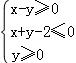
\includegraphics[width=.42\linewidth]{assets/asset-028-01.jpg}
\end{center}
\begin{choices}
  \item $3$
  \item $2\sqrt{2}$
  \item $\sqrt{5}$
  \item $2$
\end{choices}
\begin{solution}
\textbf{答案：}$A$

\textbf{分析：}如图：以$A$为原点，以$AB$，$AD$所在的直线为$x$，$y$轴建立如图所示的坐标系，先求出圆的标准方程，再设点$P$的坐标为$(\frac{2\sqrt{5}}{5}\cos\theta+1，\frac{2\sqrt{5}}{5}\sin\theta+2)$，根据$\overrightarrow{AP}=\lambda\overrightarrow{AB}+\mu\overrightarrow{AD}$，求出$\lambda$，$\mu$，根据三角函数的性质即可求出最值。

\textbf{详解：}如图：以$A$为原点，以$AB$，$AD$所在的直线为$x$，$y$轴建立如图所示的坐标系，则$A(0,0)$，$B(1,0)$，$D(0,2)$，$C(1,2)$。因为动点$P$在以点$C$为圆心且与$BD$相切的圆上，设圆的半径为$r$。因为$BC=2$，$CD=1$，所以$BD=\sqrt{BC^2+CD^2}=\sqrt{5}$。所以$\frac{1}{2}BC\cdot CD=\frac{1}{2}BD\cdot r$，所以$r=\frac{2\sqrt{5}}{5}$。所以圆的方程为$(x-1)^2+(y-2)^2=\frac{4}{5}$。设点$P$的坐标为$(\frac{2\sqrt{5}}{5}\cos\theta+1，\frac{2\sqrt{5}}{5}\sin\theta+2)$。因为$\overrightarrow{AP}=\lambda\overrightarrow{AB}+\mu\overrightarrow{AD}$，所以$(\frac{2\sqrt{5}}{5}\cos\theta+1，\frac{2\sqrt{5}}{5}\sin\theta+2)=\lambda(1,0)+\mu(0,2)=(\lambda,2\mu)$。所以$\frac{2\sqrt{5}}{5}\cos\theta+1=\lambda$，$\frac{2\sqrt{5}}{5}\sin\theta+2=2\mu$。所以$\lambda+\mu=\frac{\sqrt{5}}{5}\cos\theta+\frac{\sqrt{5}}{5}\sin\theta+2=\sin(\theta+\varphi)+2$，其中$\tan\varphi=2$。因为$-1\le\sin(\theta+\varphi)\le1$，所以$1\le\lambda+\mu\le3$，故$\lambda+\mu$的最大值为$3$。故选A。
\end{solution}
\end{question}

\begin{question}[points=12]
\textbf{来源：}2017 年 全国III卷-理科，第 17 题\quad \textbf{专题：}三角形、三角函数\par
$\triangle ABC$的内角$A$，$B$，$C$的对边分别为$a$，$b$，$c$，已知$\sin A+\sqrt{3}\cos A=0$，$a=2\sqrt{7}$，$b=2$．

（1）求$c$；

（2）设$D$为$BC$边上一点，且$AD\perp AC$，求$\triangle ABD$的面积．
\begin{solution}
\textbf{答案：}（1）$c=4$；（2）$\sqrt{3}$

\textbf{分析：}（1）先根据同角的三角函数的关系求出$A$，再根据余弦定理即可求出；（2）先根据夹角求出$\cos C$，求出$CD$的长，得到$S_{\triangle ABD}=\frac{1}{2}S_{\triangle ABC}$。

\textbf{详解：}解：（1）因为$\sin A+\sqrt{3}\cos A=0$，所以$\tan A=-\sqrt{3}$，因为$0<A<\pi$，所以$A=\frac{2\pi}{3}$。由余弦定理可得$a^2=b^2+c^2-2bc\cos A$，即$28=4+c^2-2\times2c\times(-\frac{1}{2})$，即$c^2+2c-24=0$，解得$c=-6$（舍去）或$c=4$，故$c=4$。
（2）因为$c^2=b^2+a^2-2ab\cos C$，所以$16=28+4-2\times2\sqrt{7}\times2\times\cos C$，所以$\cos C=\frac{2\sqrt{7}}{7}$，所以$CD=\frac{AC}{\cos C}=\frac{2}{\frac{2\sqrt{7}}{7}}=\sqrt{7}$。所以$CD=\frac{1}{2}BC$。因为$S_{\triangle ABC}=\frac{1}{2}AB\cdot AC\cdot\sin\angle BAC=\frac{1}{2}\times4\times2\times\frac{\sqrt{3}}{2}=2\sqrt{3}$，所以$S_{\triangle ABD}=\frac{1}{2}S_{\triangle ABC}=\sqrt{3}$。
\end{solution}
\end{question}

\begin{question}[points=5]
\textbf{来源：}2017 年 全国III卷-文科，第 4 题\quad \textbf{专题：}三角函数\par
已知$\sin\alpha-\cos\alpha=\frac{4}{3}$，则$\sin2\alpha=$（    ）
\begin{choices}
  \item A．$-\frac{7}{9}$
  \item B．$-\frac{2}{9}$
  \item C．$\frac{2}{9}$
  \item D．$\frac{7}{9}$
\end{choices}
\begin{solution}
\textbf{答案：}A

\textbf{分析：}由条件，两边平方，根据二倍角公式和平方关系即可求出。

\textbf{详解：}由$\sin\alpha-\cos\alpha=\frac{4}{3}$，平方得$1-\sin2\alpha=\frac{16}{9}$，所以$\sin2\alpha=-\frac{7}{9}$。
\end{solution}
\end{question}

\begin{question}[points=5]
\textbf{来源：}2017 年 全国III卷-文科，第 6 题\quad \textbf{专题：}三角函数\par
函数$f(x)=\frac{1}{5}\sin(x+\frac{\pi}{3})+\cos(x-\frac{\pi}{6})$的最大值为（   ）
\begin{choices}
  \item A．$\frac{6}{5}$
  \item B．$1$
  \item C．$\frac{3}{5}$
  \item D．$\frac{1}{5}$
\end{choices}
\begin{solution}
\textbf{答案：}A

\textbf{分析：}利用诱导公式化简函数的解析式，通过正弦函数的最值求解即可。

\textbf{详解：}$f(x)=\frac{1}{5}\sin(x+\frac{\pi}{3})+\cos(x-\frac{\pi}{6})=\frac{1}{5}\sin(x+\frac{\pi}{3})+\sin(x+\frac{\pi}{3})=\frac{6}{5}\sin(x+\frac{\pi}{3})$，最大值为$\frac{6}{5}$。
\end{solution}
\end{question}

\begin{question}[points=5]
\textbf{来源：}2017 年 全国III卷-文科，第 7 题\quad \textbf{专题：}三角函数\par
函数$y=1+x+\frac{\sin x}{x}$的部分图象大致为（       ）

\begin{center}
  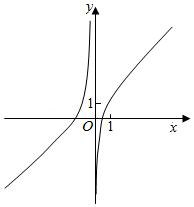
\includegraphics[width=.42\linewidth]{assets/asset-032-01.jpg}
\end{center}
\begin{choices}
  \item A．
  \item B．
  \item C．
  \item D．
\end{choices}
\begin{solution}
\textbf{答案：}D

\textbf{分析：}通过函数的解析式，利用函数的奇偶性的性质，函数的图象经过的特殊点判断函数的图象即可。

\textbf{详解：}函数$y=1+x+\frac{\sin x}{x}$，$f(x)=x+\frac{\sin x}{x}$是奇函数，图象关于原点对称，则$y=1+x+\frac{\sin x}{x}$的图象关于$(0,1)$对称，当$x\to 0^+$时$f(x)>0$，排除A、C；当$x=\pi$时$y=1+\pi$，排除B。
\end{solution}
\end{question}

\begin{question}[points=5]
\textbf{来源：}2017 年 全国III卷-文科，第 13 题\quad \textbf{专题：}向量\par
已知向量$\vec{a}=(-2,3)$，$\vec{b}=(3,m)$，且$\vec{a}\perp\vec{b}$，则$m=$        。
\fillin[{$2$}]
\begin{solution}
\textbf{答案：}$2$

\textbf{分析：}利用平面向量数量积坐标运算法则和向量垂直的性质求解。

\textbf{详解：}$\vec{a}\cdot\vec{b}=(-2)\times3+3m=0$，解得$m=2$。
\end{solution}
\end{question}

\begin{question}[points=5]
\textbf{来源：}2017 年 全国III卷-文科，第 15 题\quad \textbf{专题：}三角形\par
$\triangle ABC$的内角$A,B,C$的对边分别为$a,b,c$，已知$C=60^\circ$，$b=\sqrt{6}$，$c=3$，则$A=$        。
\fillin[{$75^\circ$}]
\begin{solution}
\textbf{答案：}$75^\circ$

\textbf{分析：}根据正弦定理和三角形的内角和计算即可。

\textbf{详解：}由正弦定理$\frac{b}{\sin B}=\frac{c}{\sin C}$，得$\sin B=\frac{b\sin C}{c}=\frac{\sqrt{6}\times\frac{\sqrt{3}}{2}}{3}=\frac{\sqrt{2}}{2}$，因为$b<c$，所以$B=45^\circ$，$A=180^\circ-60^\circ-45^\circ=75^\circ$。
\end{solution}
\end{question}

\begin{question}[points=5]
\textbf{来源：}2017 年 全国II卷-理科，第 10 题\quad \textbf{专题：}向量\par
已知直三棱柱 $ABC-A_1B_1C_1$ 中，$\angle ABC=120^\circ$，$AB=2$，$BC=CC_1=1$，则异面直线 $AB_1$ 与 $BC_1$ 所成角的余弦值为（   ）
\begin{choices}
  \item $\frac{\sqrt{15}}{5}$
  \item $\frac{\sqrt{10}}{5}$
  \item $\frac{\sqrt{10}}{5}$
  \item $\frac{\sqrt{5}}{5}$
\end{choices}
\begin{solution}
\textbf{答案：}$C$

\textbf{分析：}【解法一】设 $M$、$N$、$P$ 分别为 $AB$，$BB_1$ 和 $B_1C_1$ 的中点，得出 $AB_1$、$BC_1$ 夹角为 $MN$ 和 $NP$ 夹角或其补角；根据中位线定理，结合余弦定理求出 $AC$、$MQ$，$MP$ 和 $\angle MNP$ 的余弦值即可．【解法二】通过补形的办法，把原来的直三棱柱变成直四棱柱，解法更简洁。

\textbf{详解：}【解法一】如图所示，设 $M$、$N$、$P$ 分别为 $AB$，$BB_1$ 和 $B_1C_1$ 的中点，则 $AB_1$、$BC_1$ 夹角为 $MN$ 和 $NP$ 夹角或其补角（因异面直线所成角为 $(0,\frac{\pi}{2}]$），可知 $MN=\frac{1}{2}AB_1=\frac{\sqrt{5}}{2}$，$NP=\frac{1}{2}BC_1=\frac{\sqrt{2}}{2}$；作 $BC$ 中点 $Q$，则 $\triangle PQM$ 为直角三角形；$\because PQ=1$，$MQ=\frac{1}{2}AC$，$\triangle ABC$ 中，由余弦定理得 $AC^2=AB^2+BC^2-2AB\cdot BC\cdot\cos\angle ABC=4+1-2\times2\times1\times(-\frac{1}{2})=7$，$\therefore AC=\sqrt{7}$，$\therefore MQ=\frac{\sqrt{7}}{2}$；在 $\triangle MQP$ 中，$MP=\sqrt{PQ^2+MQ^2}=\frac{\sqrt{11}}{2}$；在 $\triangle PMN$ 中，由余弦定理得 $\cos\angle MNP=\frac{MN^2+NP^2-PM^2}{2\cdot MN\cdot NP}=\frac{\frac{5}{4}+\frac{1}{2}-\frac{11}{4}}{2\times\frac{\sqrt{5}}{2}\times\frac{\sqrt{2}}{2}}=\frac{-\frac{1}{2}}{\sqrt{10}}=-\frac{\sqrt{10}}{10}$；又异面直线所成角的范围是 $(0,\frac{\pi}{2}]$，$\therefore AB_1$ 与 $BC_1$ 所成角的余弦值为 $\frac{\sqrt{10}}{5}$．【解法二】如图所示，补成四棱柱 $ABCD-A_1B_1C_1D_1$，求 $\angle BC_1D$ 即可；$BC_1=\sqrt{2}$，$BD=\sqrt{1^2+1^2-2\times1\times1\times\cos60^\circ}=1$，$C_1D=\sqrt{5}$，$\because BC_1^2+BD^2=C_1D^2$，$\therefore\angle DBC_1=90^\circ$，$\therefore\cos\angle BC_1D=\frac{BC_1}{C_1D}=\frac{\sqrt{2}}{\sqrt{5}}=\frac{\sqrt{10}}{5}$．故选：$C$。
\end{solution}
\end{question}

\begin{question}[points=5]
\textbf{来源：}2017 年 全国II卷-理科，第 12 题\quad \textbf{专题：}向量\par
已知 $\triangle ABC$ 是边长为 $2$ 的等边三角形，$P$ 为平面 $ABC$ 内一点，则 $\overrightarrow{PA}\cdot(\overrightarrow{PB}+\overrightarrow{PC})$ 的最小值是（   ）
\begin{choices}
  \item $-2$
  \item $-\frac{3}{2}$
  \item $-\frac{4}{3}$
  \item $-1$
\end{choices}
\begin{solution}
\textbf{答案：}$B$

\textbf{分析：}根据条件建立坐标系，求出点的坐标，利用坐标法结合向量数量积的公式进行计算即可。

\textbf{详解：}建立如图所示的坐标系，以 $BC$ 中点为坐标原点，则 $A(0,\sqrt{3})$，$B(-1,0)$，$C(1,0)$，设 $P(x,y)$，则 $\overrightarrow{PA}=(-x,\sqrt{3}-y)$，$\overrightarrow{PB}=(-1-x,-y)$，$\overrightarrow{PC}=(1-x,-y)$，则 $\overrightarrow{PA}\cdot(\overrightarrow{PB}+\overrightarrow{PC})=2x^2-2\sqrt{3}y+2y^2=2[x^2+(y-\frac{\sqrt{3}}{2})^2-\frac{3}{4}]$，$\therefore$ 当 $x=0$，$y=\frac{\sqrt{3}}{2}$ 时，取得最小值 $2\times(-\frac{3}{4})=-\frac{3}{2}$，故选：$B$。
\end{solution}
\end{question}

\begin{question}[points=5]
\textbf{来源：}2017 年 全国II卷-理科，第 14 题\quad \textbf{专题：}三角函数\par
函数 $f(x)=\sin^2x+\sqrt{3}\cos x-\frac{3}{4}$（$x\in[0,\frac{\pi}{2}]$）的最大值是 ．
\fillin[{$1$}]
\begin{solution}
\textbf{答案：}$1$

\textbf{分析：}同角的三角函数的关系以及二次函数的性质即可求出。

\textbf{详解：}$f(x)=\sin^2x+\sqrt{3}\cos x-\frac{3}{4}=1-\cos^2x+\sqrt{3}\cos x-\frac{3}{4}$，令 $\cos x=t$ 且 $t\in[0,1]$，则 $y=-t^2+\sqrt{3}t+\frac{1}{4}=-(t-\frac{\sqrt{3}}{2})^2+1$，当 $t=\frac{\sqrt{3}}{2}$ 时，$f(t)_{\max}=1$，即 $f(x)$ 的最大值为 $1$，故答案为：$1$。
\end{solution}
\end{question}

\begin{question}[points=12]
\textbf{来源：}2017 年 全国II卷-理科，第 17 题\quad \textbf{专题：}三角形、三角函数\par
$\triangle ABC$ 的内角 $A$，$B$，$C$ 的对边分别为 $a$，$b$，$c$，已知 $\sin(A+C)=8\sin^2\frac{B}{2}$．

（1）求 $\cos B$；

（2）若 $a+c=6$，$\triangle ABC$ 的面积为 $2$，求 $b$．
\begin{solution}
\textbf{答案：}（1）$\cos B=\frac{15}{17}$；（2）$b=2$

\textbf{分析：}（1）利用三角形的内角和定理可知 $A+C=\pi-B$，再利用诱导公式化简 $\sin(A+C)$，利用降幂公式化简 $8\sin^2\frac{B}{2}$，结合 $\sin^2B+\cos^2B=1$，求出 $\cos B$，（2）由（1）可知 $\sin B=\frac{8}{17}$，利用勾面积公式求出 $ac$，再利用余弦定理即可求出 $b$。

\textbf{详解：}（1）$\sin(A+C)=8\sin^2\frac{B}{2}$，$\therefore\sin B=4(1-\cos B)$，$\because\sin^2B+\cos^2B=1$，$\therefore16(1-\cos B)^2+\cos^2B=1$，$\therefore16(1-\cos B)^2+\cos^2B-1=0$，$\therefore16(\cos B-1)^2+(\cos B-1)(\cos B+1)=0$，$\therefore(17\cos B-15)(\cos B-1)=0$，$\therefore\cos B=\frac{15}{17}$；
（2）由（1）可知 $\sin B=\frac{8}{17}$，$\because S_{\triangle ABC}=\frac{1}{2}ac\cdot\sin B=2$，$\therefore ac=\frac{17}{2}$，$\therefore b^2=a^2+c^2-2ac\cos B=a^2+c^2-2\times\frac{17}{2}\times\frac{15}{17}=a^2+c^2-15=(a+c)^2-2ac-15=36-17-15=4$，$\therefore b=2$。
\end{solution}
\end{question}

\begin{question}[points=12]
\textbf{来源：}2017 年 全国II卷-理科，第 20 题\quad \textbf{专题：}向量\par
设 $O$ 为坐标原点，动点 $M$ 在椭圆 $C:\frac{x^2}{2}+y^2=1$ 上，过 $M$ 作 $x$ 轴的垂线，垂足为 $N$，点 $P$ 满足 $\overrightarrow{NP}=\sqrt{2}\overrightarrow{NM}$．

（1）求点 $P$ 的轨迹方程；

（2）设点 $Q$ 在直线 $x=-3$ 上，且 $\overrightarrow{OP}\cdot\overrightarrow{PQ}=1$．证明：过点 $P$ 且垂直于 $OQ$ 的直线 $l$ 过 $C$ 的左焦点 $F$．
\begin{solution}
\textbf{答案：}（1）$x^2+y^2=2$；（2）略

\textbf{分析：}（1）设 $M(x_0,y_0)$，由题意可得 $N(x_0,0)$，设 $P(x,y)$，运用向量的坐标运算，结合 $M$ 满足椭圆方程，化简整理可得 $P$ 的轨迹方程；（2）设 $Q(-3,m)$，$P(\sqrt{2}\cos\alpha,\sin\alpha)$，$0\le\alpha<2\pi$，运用向量的数量积的坐标表示，可得 $m$，即有 $Q$ 的坐标，求得椭圆的左焦点坐标，求得 $OQ$，$PF$ 的斜率，由两直线垂直的条件：向量数量积为 $0$，即可得证。

\textbf{详解：}（1）设 $M(x_0,y_0)$，由题意可得 $N(x_0,0)$，设 $P(x,y)$，由点 $P$ 满足 $\overrightarrow{NP}=\sqrt{2}\overrightarrow{NM}$．可得 $(x-x_0,y)=\sqrt{2}(0,y_0)$，可得 $x-x_0=0$，$y=\sqrt{2}y_0$，即有 $x_0=x$，$y_0=\frac{y}{\sqrt{2}}$，代入椭圆方程 $\frac{x^2}{2}+y^2=1$，可得 $\frac{x^2}{2}+\frac{y^2}{2}=1$，即有点 $P$ 的轨迹方程为圆 $x^2+y^2=2$；
（2）证明：设 $Q(-3,m)$，$P(\sqrt{2}\cos\alpha,\sin\alpha)$（$0\le\alpha<2\pi$），$\overrightarrow{OP}\cdot\overrightarrow{PQ}=1$，可得 $(\sqrt{2}\cos\alpha,\sin\alpha)\cdot(-3-\sqrt{2}\cos\alpha,m-\sin\alpha)=1$，即为 $-3\sqrt{2}\cos\alpha-2\cos^2\alpha+\sqrt{2}m\sin\alpha-2\sin^2\alpha=1$，当 $\alpha=0$ 时，上式不成立，则 $0<\alpha<2\pi$，解得 $m=\frac{3(1+\sqrt{2}\cos\alpha)}{\sqrt{2}\sin\alpha}$，即有 $Q(-3,\frac{3(1+\sqrt{2}\cos\alpha)}{\sqrt{2}\sin\alpha})$，椭圆 $\frac{x^2}{2}+y^2=1$ 的左焦点 $F(-1,0)$，由 $\overrightarrow{PF}\cdot\overrightarrow{OQ}=(-1-\sqrt{2}\cos\alpha,-\sin\alpha)\cdot(-3,\frac{3(1+\sqrt{2}\cos\alpha)}{\sqrt{2}\sin\alpha})=3+3\sqrt{2}\cos\alpha-3(1+\sqrt{2}\cos\alpha)=0$．可得过点 $P$ 且垂直于 $OQ$ 的直线 $l$ 过 $C$ 的左焦点 $F$．
\end{solution}
\end{question}

\begin{question}[points=5]
\textbf{来源：}2017 年 全国II卷-文科，第 3 题\quad \textbf{专题：}三角函数\par
函数 $f(x)=\sin\left(2x+\frac{\pi}{3}\right)$ 的最小正周期为
\begin{choices}
  \item $4\pi$
  \item $2\pi$
  \item $\pi$
  \item $\frac{\pi}{2}$
\end{choices}
\begin{solution}
\textbf{答案：}$\pi$

\textbf{分析：}利用三角函数周期公式, 直接求解即可.

\textbf{详解：}函数 $f(x)=\sin\left(2x+\frac{\pi}{3}\right)$ 的最小正周期为 $\frac{2\pi}{2}=\pi$. 故选C.
\end{solution}
\end{question}

\begin{question}[points=5]
\textbf{来源：}2017 年 全国II卷-文科，第 4 题\quad \textbf{专题：}向量\par
设非零向量 $\vec{a}$, $\vec{b}$ 满足 $|\vec{a}+\vec{b}|=|\vec{a}-\vec{b}|$, 则
\begin{choices}
  \item $\vec{a}\perp\vec{b}$
  \item $|\vec{a}|=|\vec{b}|$
  \item $\vec{a}\parallel\vec{b}$
  \item $|\vec{a}|>|\vec{b}|$
\end{choices}
\begin{solution}
\textbf{答案：}$\vec{a}\perp\vec{b}$

\textbf{分析：}由已知得 $(\vec{a}+\vec{b})^2=(\vec{a}-\vec{b})^2$, 从而 $\vec{a}\cdot\vec{b}=0$, 由此得到 $\vec{a}\perp\vec{b}$.

\textbf{详解：}$\because$ 非零向量 $\vec{a}$, $\vec{b}$ 满足 $|\vec{a}+\vec{b}|=|\vec{a}-\vec{b}|$, $\therefore (\vec{a}+\vec{b})^2=(\vec{a}-\vec{b})^2$, $\therefore \vec{a}^2+2\vec{a}\cdot\vec{b}+\vec{b}^2=\vec{a}^2-2\vec{a}\cdot\vec{b}+\vec{b}^2$, 解得 $\vec{a}\cdot\vec{b}=0$, $\therefore \vec{a}\perp\vec{b}$. 故选A.
\end{solution}
\end{question}

\begin{question}[points=5]
\textbf{来源：}2017 年 全国II卷-文科，第 13 题\quad \textbf{专题：}三角函数\par
函数 $f(x)=2\cos x+\sin x$ 的最大值为
\fillin[{$\sqrt{5}$}]
\begin{solution}
\textbf{答案：}$\sqrt{5}$

\textbf{分析：}利用辅助角公式化简函数的解析式, 通过正弦函数的有界性求解即可.

\textbf{详解：}函数 $f(x)=2\cos x+\sin x=\sqrt{5}\left(\frac{2}{\sqrt{5}}\cos x+\frac{1}{\sqrt{5}}\sin x\right)=\sqrt{5}\sin(x+\theta)$, 其中 $\tan\theta=2$, 可知函数的最大值为 $\sqrt{5}$. 故答案为 $\sqrt{5}$.
\end{solution}
\end{question}

\begin{question}[points=5]
\textbf{来源：}2017 年 全国II卷-文科，第 16 题\quad \textbf{专题：}三角形、三角函数\par
$\triangle ABC$ 的内角 $A$, $B$, $C$ 的对边分别为 $a$, $b$, $c$, 若 $2b\cos B=a\cos C+c\cos A$, 则 $B=$
\fillin[{$\frac{\pi}{3}$}]
\begin{solution}
\textbf{答案：}$\frac{\pi}{3}$

\textbf{分析：}根据正弦定理和两角和的正弦公式和诱导公式计算即可.

\textbf{详解：}$\because 2b\cos B=a\cos C+c\cos A$, 由正弦定理可得, $2\cos B\sin B=\sin A\cos C+\sin C\cos A=\sin(A+C)=\sin B$, $\because \sin B\neq0$, $\therefore \cos B=\frac{1}{2}$, $\because 0<B<\pi$, $\therefore B=\frac{\pi}{3}$. 故答案为 $\frac{\pi}{3}$.
\end{solution}
\end{question}

\begin{question}[points=12]
\textbf{来源：}2017 年 全国II卷-文科，第 20 题\quad \textbf{专题：}向量\par
设 $O$ 为坐标原点, 动点 $M$ 在椭圆 $C: \frac{x^2}{2}+y^2=1$ 上, 过 $M$ 作 $x$ 轴的垂线, 垂足为 $N$, 点 $P$ 满足 $\overrightarrow{NP}=\sqrt{2}\overrightarrow{NM}$. \\ (1) 求点 $P$ 的轨迹方程; \\ (2) 设点 $Q$ 在直线 $x=-3$ 上, 且 $\overrightarrow{OP}\cdot\overrightarrow{PQ}=1$. 证明: 过点 $P$ 且垂直于 $OQ$ 的直线 $l$ 过 $C$ 的左焦点 $F$.
\begin{solution}

\textbf{分析：}(1) 设 $M(x_0,y_0)$, 由题意可得 $N(x_0,0)$, 设 $P(x,y)$, 运用向量的坐标运算, 结合 $M$ 满足椭圆方程, 化简整理可得 $P$ 的轨迹方程; (2) 设 $Q(-3,m)$, $P(\sqrt{2}\cos\alpha,\sin\alpha)$ $(0\le\alpha<2\pi)$, 运用向量的数量积的坐标表示, 可得 $m$, 即有 $Q$ 的坐标, 求得椭圆的左焦点坐标, 求得 $OQ$, $PF$ 的斜率, 由两直线垂直的条件: 向量数量积为 $0$, 即可得证.

\textbf{详解：}(1) 设 $M(x_0,y_0)$, 由题意可得 $N(x_0,0)$, 设 $P(x,y)$, 由点 $P$ 满足 $\overrightarrow{NP}=\sqrt{2}\overrightarrow{NM}$, 可得 $(x-x_0,y)=\sqrt{2}(0,y_0)$, 可得 $x-x_0=0$, $y=\sqrt{2}y_0$, 即有 $x_0=x$, $y_0=\frac{\sqrt{2}}{2}y$, 代入椭圆方程 $\frac{x^2}{2}+y^2=1$, 可得 $\frac{x^2}{2}+\frac{y^2}{2}=1$, 即有点 $P$ 的轨迹方程为圆 $x^2+y^2=2$; \\ (2) 证明: 设 $Q(-3,m)$, $P(\sqrt{2}\cos\alpha,\sin\alpha)$ $(0\le\alpha<2\pi)$, $\overrightarrow{OP}\cdot\overrightarrow{PQ}=1$, 可得 $(\sqrt{2}\cos\alpha,\sin\alpha)\cdot(-3-\sqrt{2}\cos\alpha,m-\sin\alpha)=1$, 即为 $-3\sqrt{2}\cos\alpha-2\cos^2\alpha+\sqrt{2}m\sin\alpha-2\sin^2\alpha=1$, 当 $\alpha=0$ 时, 上式不成立, 则 $0<\alpha<2\pi$, 解得 $m=\frac{3\sqrt{2}\cos\alpha+3}{\sqrt{2}\sin\alpha}$, 即有 $Q\left(-3,\frac{3\sqrt{2}\cos\alpha+3}{\sqrt{2}\sin\alpha}\right)$, 椭圆 $\frac{x^2}{2}+y^2=1$ 的左焦点 $F(-1,0)$, 由 $\overrightarrow{PF}\cdot\overrightarrow{OQ}=(-1-\sqrt{2}\cos\alpha,-\sin\alpha)\cdot\left(-3,\frac{3\sqrt{2}\cos\alpha+3}{\sqrt{2}\sin\alpha}\right)=3+3\sqrt{2}\cos\alpha-3(1+\sqrt{2}\cos\alpha)=0$. 可得过点 $P$ 且垂直于 $OQ$ 的直线 $l$ 过 $C$ 的左焦点 $F$.
\end{solution}
\end{question}

\begin{question}[points=5]
\textbf{来源：}2017 年 全国I卷-理科，第 9 题\quad \textbf{专题：}三角函数\par
已知曲线 $C_1:y=\cos x$，$C_2:y=\sin\left(2x+\frac{2\pi}{3}\right)$，则下面结论正确的是（ ）
\begin{choices}
  \item 把 $C_1$ 上各点的横坐标伸长到原来的 2 倍，纵坐标不变，再把得到的曲线向右平移 $\frac{\pi}{6}$ 个单位长度，得到曲线 $C_2$
  \item 把 $C_1$ 上各点的横坐标伸长到原来的 2 倍，纵坐标不变，再把得到的曲线向左平移 $\frac{\pi}{12}$ 个单位长度，得到曲线 $C_2$
  \item 把 $C_1$ 上各点的横坐标缩短到原来的 $\frac{1}{2}$ 倍，纵坐标不变，再把得到的曲线向右平移 $\frac{\pi}{6}$ 个单位长度，得到曲线 $C_2$
  \item 把 $C_1$ 上各点的横坐标缩短到原来的 $\frac{1}{2}$ 倍，纵坐标不变，再把得到的曲线向左平移 $\frac{\pi}{12}$ 个单位长度，得到曲线 $C_2$
\end{choices}
\begin{solution}
\textbf{答案：}D

\textbf{分析：}利用三角函数的伸缩变换以及平移变换转化求解即可．

\textbf{详解：}把 $C_1$ 上各点的横坐标缩短到原来的 $\frac{1}{2}$ 倍，纵坐标不变，得到函数 $y=\cos 2x$ 图象，再把得到的曲线向左平移 $\frac{\pi}{12}$ 个单位长度，得到函数 $y=\cos\left[2\left(x+\frac{\pi}{12}\right)\right]=\cos\left(2x+\frac{\pi}{6}\right)=\sin\left(2x+\frac{2\pi}{3}\right)$ 的图象，即曲线 $C_2$．故选：D．
\end{solution}
\end{question}

\begin{question}[points=5]
\textbf{来源：}2017 年 全国I卷-理科，第 13 题\quad \textbf{专题：}向量\par
已知向量 $\vec{a}$，$\vec{b}$ 的夹角为 $60^\circ$，$|\vec{a}|=2$，$|\vec{b}|=1$，则 $|\vec{a}+2\vec{b}|=$ ．
\fillin[{$2\sqrt{3}$}]
\begin{solution}
\textbf{答案：}$2\sqrt{3}$

\textbf{分析：}根据平面向量的数量积求出模长即可．

\textbf{详解：}【解法一】向量 $\vec{a}$，$\vec{b}$ 的夹角为 $60^\circ$，且 $|\vec{a}|=2$，$|\vec{b}|=1$，所以$|\vec{a}+2\vec{b}|^2=|\vec{a}|^2+4\vec{a}\cdot\vec{b}+4|\vec{b}|^2=2^2+4\times2\times1\times\cos60^\circ+4\times1^2=4+4+4=12$，所以$|\vec{a}+2\vec{b}|=2\sqrt{3}$．【解法二】根据题意画出图形，如图所示；结合图形 $\overrightarrow{OC}=\overrightarrow{OA}+\overrightarrow{OB}=\vec{a}+2\vec{b}$；在 $\triangle OAC$ 中，由余弦定理得 $|\overrightarrow{OC}|=\sqrt{2^2+2^2-2\times2\times2\times\cos120^\circ}=2\sqrt{3}$，即 $|\vec{a}+2\vec{b}|=2\sqrt{3}$．故答案为：$2\sqrt{3}$．
\end{solution}
\end{question}

\begin{question}[points=12]
\textbf{来源：}2017 年 全国I卷-理科，第 17 题\quad \textbf{专题：}三角形、三角函数\par
$\triangle ABC$ 的内角 $A$，$B$，$C$ 的对边分别为 $a$，$b$，$c$，已知 $\triangle ABC$ 的面积为 $\frac{a^2}{3\sin A}$．

（1）求 $\sin B\sin C$；

（2）若 $6\cos B\cos C=1$，$a=3$，求 $\triangle ABC$ 的周长．
\begin{solution}
\textbf{答案：}（1）$\frac{2}{3}$；（2）$3+\sqrt{33}$

\textbf{分析：}（1）根据三角形面积公式和正弦定理可得答案，（2）根据两角余弦公式可得 $\cos A=\frac{1}{2}$，即可求出 $A=\frac{\pi}{3}$，再根据正弦定理可得 $bc=8$，根据余弦定理即可求出 $b+c$，问题得以解决．

\textbf{详解：}解：（1）由三角形的面积公式可得 $S_{\triangle ABC}=\frac{1}{2}ac\sin B=\frac{a^2}{3\sin A}$，所以$3c\sin B\sin A=2a$，由正弦定理可得 $3\sin C\sin B\sin A=2\sin A$，因为$\sin A\neq0$，所以$\sin B\sin C=\frac{2}{3}$．
（2）因为$6\cos B\cos C=1$，所以$\cos B\cos C=\frac{1}{6}$，所以$\cos B\cos C-\sin B\sin C=\frac{1}{6}-\frac{2}{3}=-\frac{1}{2}$，所以$\cos(B+C)=-\frac{1}{2}$，所以$\cos A=\frac{1}{2}$，因为$0<A<\pi$，所以$A=\frac{\pi}{3}$，因为$\frac{a}{\sin A}=\frac{b}{\sin B}=\frac{c}{\sin C}=2R=\frac{3}{\frac{\sqrt{3}}{2}}=2\sqrt{3}$，所以$\sin B\sin C=\frac{b}{2\sqrt{3}}\cdot\frac{c}{2\sqrt{3}}=\frac{bc}{12}=\frac{2}{3}$，所以$bc=8$，因为$a^2=b^2+c^2-2bc\cos A$，所以$b^2+c^2-bc=9$，所以$(b+c)^2=9+3cb=9+24=33$，所以$b+c=\sqrt{33}$，所以周长 $a+b+c=3+\sqrt{33}$．
\end{solution}
\end{question}

\begin{question}[points=5]
\textbf{来源：}2017 年 全国I卷-文科，第 8 题\quad \textbf{专题：}三角函数\par
函数$y=\frac{\sin x}{1+\cos x}$的部分图象大致为（        ）

\begin{center}
  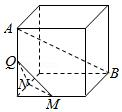
\includegraphics[width=.42\linewidth]{assets/asset-048-01.jpg}
\end{center}
\begin{choices}
  \item 
  \item 
  \item 
  \item 
\end{choices}
\begin{solution}
\textbf{答案：}C

\textbf{分析：}判断函数的奇偶性排除选项，利用特殊值判断即可。

\textbf{详解：}解：函数$y=\frac{\sin x}{1+\cos x}$，可知函数是奇函数，排除选项B，当$x=\frac{\pi}{2}$时，$f(\frac{\pi}{2})=\frac{1}{1+0}=1$，排除A，$x=\pi$时，$f(\pi)=0$，排除D。故选：C。
\end{solution}
\end{question}

\begin{question}[points=5]
\textbf{来源：}2017 年 全国I卷-文科，第 11 题\quad \textbf{专题：}三角形、三角函数\par
$\triangle ABC$的内角$A$，$B$，$C$的对边分别为$a$，$b$，$c$，已知$\sin B+\sin A(\sin C-\cos C)=0$，$a=2$，$c=\sqrt{2}$，则$C=$（    ）
\begin{choices}
  \item $\frac{\pi}{12}$
  \item $\frac{\pi}{6}$
  \item $\frac{\pi}{4}$
  \item $\frac{\pi}{3}$
\end{choices}
\begin{solution}
\textbf{答案：}B

\textbf{分析：}根据诱导公式和两角和的正弦公式以及正弦定理计算即可。

\textbf{详解：}解：$\sin B=\sin(A+C)=\sin A\cos C+\cos A\sin C$，$\because\sin B+\sin A(\sin C-\cos C)=0$，$\therefore\sin A\cos C+\cos A\sin C+\sin A\sin C-\sin A\cos C=0$，$\therefore\cos A\sin C+\sin A\sin C=0$，$\because\sin C\neq 0$，$\therefore\cos A=-\sin A$，$\therefore\tan A=-1$，$\because\frac{\pi}{2}<A<\pi$，$\therefore A=\frac{3\pi}{4}$，由正弦定理可得$\frac{a}{\sin A}=\frac{c}{\sin C}$，$\therefore\sin C=\frac{c\sin A}{a}$，$\because a=2$，$c=\sqrt{2}$，$\therefore\sin C=\frac{\sqrt{2}\times\frac{\sqrt{2}}{2}}{2}=\frac{1}{2}$，$\because a>c$，$\therefore C=\frac{\pi}{6}$，故选：B。
\end{solution}
\end{question}

\begin{question}[points=5]
\textbf{来源：}2017 年 全国I卷-文科，第 13 题\quad \textbf{专题：}向量\par
已知向量$\vec{a}=(-1,2)$，$\vec{b}=(m,1)$，若向量$\vec{a}+\vec{b}$与$\vec{a}$垂直，则$m=$ ．
\fillin[{$7$}]
\begin{solution}
\textbf{答案：}$7$

\textbf{分析：}利用平面向量坐标运算法则先求出$\vec{a}+\vec{b}$，再由向量$\vec{a}+\vec{b}$与$\vec{a}$垂直，利用向量垂直的条件能求出$m$的值。

\textbf{详解：}解：$\because$向量$\vec{a}=(-1,2)$，$\vec{b}=(m,1)$，$\therefore\vec{a}+\vec{b}=(-1+m,3)$，$\because$向量$\vec{a}+\vec{b}$与$\vec{a}$垂直，$\therefore(\vec{a}+\vec{b})\cdot\vec{a}=(-1+m)\times(-1)+3\times2=0$，解得$m=7$。故答案为：7。
\end{solution}
\end{question}

\begin{question}[points=5]
\textbf{来源：}2017 年 全国I卷-文科，第 15 题\quad \textbf{专题：}三角函数\par
已知$\alpha\in(0,\frac{\pi}{2})$，$\tan\alpha=2$，则$\cos(\alpha-\frac{\pi}{4})=$ ．
\fillin[{$\frac{3\sqrt{10}}{10}$}]
\begin{solution}
\textbf{答案：}$\frac{3\sqrt{10}}{10}$

\textbf{分析：}根据同角的三角函数的关系求出$\sin\alpha=\frac{2\sqrt{5}}{5}$，$\cos\alpha=\frac{\sqrt{5}}{5}$，再根据两角差的余弦公式即可求出。

\textbf{详解：}解：$\because\alpha\in(0,\frac{\pi}{2})$，$\tan\alpha=2$，$\therefore\sin\alpha=2\cos\alpha$，$\because\sin^2\alpha+\cos^2\alpha=1$，解得$\sin\alpha=\frac{2\sqrt{5}}{5}$，$\cos\alpha=\frac{\sqrt{5}}{5}$，$\therefore\cos(\alpha-\frac{\pi}{4})=\cos\alpha\cos\frac{\pi}{4}+\sin\alpha\sin\frac{\pi}{4}=\frac{\sqrt{5}}{5}\times\frac{\sqrt{2}}{2}+\frac{2\sqrt{5}}{5}\times\frac{\sqrt{2}}{2}=\frac{3\sqrt{10}}{10}$，故答案为：$\frac{3\sqrt{10}}{10}$。
\end{solution}
\end{question}

\section*{2018 年}

\begin{question}[points=5]
\textbf{来源：}2018 年 全国III卷-理科，第 4 题\quad \textbf{专题：}三角函数\par
若$\sin\alpha=\frac{1}{3}$，则$\cos2\alpha=$（ ）
\begin{choices}
  \item $\frac{8}{9}$
  \item $\frac{7}{9}$
  \item $-\frac{7}{9}$
  \item $-\frac{8}{9}$
\end{choices}
\begin{solution}
\textbf{答案：}B

\textbf{分析：}$\cos2\alpha=1-2\sin^2\alpha$，由此能求出结果．

\textbf{详解：}$\because \sin\alpha=\frac{1}{3}$，$\therefore \cos2\alpha=1-2\sin^2\alpha=1-2\times\frac{1}{9}=\frac{7}{9}$．
\end{solution}
\end{question}

\begin{question}[points=5]
\textbf{来源：}2018 年 全国III卷-理科，第 9 题\quad \textbf{专题：}三角形、三角函数\par
$\triangle ABC$的内角$A$，$B$，$C$的对边分别为$a$，$b$，$c$．若$\triangle ABC$的面积为$\frac{a^2+b^2-c^2}{4}$，则$C=$（ ）
\begin{choices}
  \item $\frac{\pi}{2}$
  \item $\frac{\pi}{3}$
  \item $\frac{\pi}{4}$
  \item $\frac{\pi}{6}$
\end{choices}
\begin{solution}
\textbf{答案：}C

\textbf{分析：}利用三角形面积公式和余弦定理求解．

\textbf{详解：}$S_{\triangle ABC}=\frac{1}{2}ab\sin C = \frac{a^2+b^2-c^2}{4} = \frac{2ab\cos C}{4} = \frac{ab\cos C}{2}$，所以$\sin C = \cos C$，又$0<C<\pi$，故$C=\frac{\pi}{4}$．
\end{solution}
\end{question}

\begin{question}[points=5]
\textbf{来源：}2018 年 全国III卷-理科，第 13 题\quad \textbf{专题：}向量\par
已知向量$\vec{a}=(1,2)$，$\vec{b}=(2,-2)$，$\vec{c}=(1,\lambda)$．若$\vec{c}\parallel(2\vec{a}+\vec{b})$，则$\lambda=$．
\fillin[{$\frac{1}{2}$}]
\begin{solution}
\textbf{答案：}$\frac{1}{2}$

\textbf{分析：}利用向量坐标运算法则求出$2\vec{a}+\vec{b}$，再由向量平行的性质能求出$\lambda$．

\textbf{详解：}$2\vec{a}+\vec{b}=2(1,2)+(2,-2)=(4,2)$，$\because \vec{c}\parallel(2\vec{a}+\vec{b})$，$\therefore$设$\vec{c}=k(4,2)$，即$(1,\lambda)=k(4,2)$，解得$k=\frac{1}{4}$，$\lambda=2k=\frac{1}{2}$．
\end{solution}
\end{question}

\begin{question}[points=5]
\textbf{来源：}2018 年 全国III卷-理科，第 15 题\quad \textbf{专题：}三角函数\par
函数$f(x)=\cos(3x+\frac{\pi}{6})$在$[0,\pi]$的零点个数为．
\fillin[{$3$}]
\begin{solution}
\textbf{答案：}$3$

\textbf{分析：}解方程$\cos(3x+\frac{\pi}{6})=0$，求得$x$在$[0,\pi]$内的个数．

\textbf{详解：}由$f(x)=0$得$3x+\frac{\pi}{6}=\frac{\pi}{2}+k\pi$，$k\in\mathbb{Z}$，即$x=\frac{\pi}{9}+\frac{k\pi}{3}$．当$k=0$，$x=\frac{\pi}{9}\in[0,\pi]$；$k=1$，$x=\frac{4\pi}{9}\in[0,\pi]$；$k=2$，$x=\frac{7\pi}{9}\in[0,\pi]$；$k=3$，$x=\frac{10\pi}{9}\notin[0,\pi]$，故零点个数为3．
\end{solution}
\end{question}

\begin{question}[points=12]
\textbf{来源：}2018 年 全国III卷-理科，第 20 题\quad \textbf{专题：}向量\par
已知斜率为$k$的直线$l$与椭圆$C:\frac{x^2}{4}+\frac{y^2}{3}=1$交于$A$，$B$两点，线段$AB$的中点为$M(1,m)$（$m>0$）．

（1）证明：$k<-\frac{1}{2}$；

（2）设$F$为$C$的右焦点，$P$为$C$上一点，且$\overrightarrow{FP}+\overrightarrow{FA}+\overrightarrow{FB}=0$．证明：$|\overrightarrow{FA}|$，$|\overrightarrow{FP}|$，$|\overrightarrow{FB}|$成等差数列，并求该数列的公差．
\begin{solution}

\textbf{分析：}（1）设$A(x_1,y_1)$，$B(x_2,y_2)$，利用点差法得到$k$与$m$的关系，再由$M$在椭圆内得$m$的范围，从而证明$k<-\frac{1}{2}$．（2）利用向量关系求出$P$点坐标，结合椭圆焦半径公式证明等差数列，并求公差．

\textbf{详解：}（1）设$A(x_1,y_1)$，$B(x_2,y_2)$，则$x_1+x_2=2$，$y_1+y_2=2m$，代入椭圆方程相减得$\frac{x_1^2-x_2^2}{4}+\frac{y_1^2-y_2^2}{3}=0$，即$\frac{(x_1+x_2)(x_1-x_2)}{4}+\frac{(y_1+y_2)(y_1-y_2)}{3}=0$，所以$\frac{2(x_1-x_2)}{4}+\frac{2m(y_1-y_2)}{3}=0$，解得$k=\frac{y_1-y_2}{x_1-x_2}=-\frac{3}{4m}$．由$M(1,m)$在椭圆内得$\frac{1}{4}+\frac{m^2}{3}<1$，解得$0<m<\frac{3}{2}$，故$k=-\frac{3}{4m}<-\frac{1}{2}$．
（2）设$P(x_3,y_3)$，由$\overrightarrow{FP}+\overrightarrow{FA}+\overrightarrow{FB}=0$得$(x_3-1,y_3)+(x_1-1,y_1)+(x_2-1,y_2)=(0,0)$，所以$x_3=1$，$y_3=-(y_1+y_2)=-2m$，代入椭圆得$\frac{1}{4}+\frac{4m^2}{3}=1$，解得$m=\frac{3}{4}$（负舍），故$k=-1$．椭圆右焦点$F(1,0)$，离心率$e=\frac{1}{2}$，焦半径$|FA|=a-ex_1=2-\frac{1}{2}x_1$，$|FB|=2-\frac{1}{2}x_2$，$|FP|=2-\frac{1}{2}x_3=2-\frac{1}{2}=\frac{3}{2}$，$|FA|+|FB|=4-\frac{1}{2}(x_1+x_2)=4-1=3=2\times\frac{3}{2}=2|FP|$，所以$|FA|$，$|FP|$，$|FB|$成等差数列．设直线$AB$方程为$y=-(x-1)$，联立椭圆得$7x^2-8x-8=0$，则$x_1+x_2=\frac{8}{7}$，$x_1x_2=-\frac{8}{7}$，$|x_1-x_2|=\sqrt{(x_1+x_2)^2-4x_1x_2}=\sqrt{\frac{64}{49}+\frac{32}{7}}=\frac{12\sqrt{2}}{7}$，公差$d=\frac{1}{2}|(|FA|-|FB|)|=\frac{1}{2}|(2-\frac{1}{2}x_1)-(2-\frac{1}{2}x_2)|=\frac{1}{4}|x_1-x_2|=\frac{3\sqrt{2}}{7}$，所以公差为$\pm\frac{3\sqrt{2}}{7}$．
\end{solution}
\end{question}

\begin{question}[points=5]
\textbf{来源：}2018 年 全国III卷-文科，第 4 题\quad \textbf{专题：}三角函数\par
若 $\sin\alpha = \frac{1}{3}$，则 $\cos2\alpha =$
\begin{choices}
  \item $\frac{8}{9}$
  \item $\frac{7}{9}$
  \item $-\frac{7}{9}$
  \item $-\frac{8}{9}$
\end{choices}
\begin{solution}
\textbf{答案：}B

\textbf{分析：}$\cos2\alpha=1-2\sin^2\alpha$，由此能求出结果．

\textbf{详解：}$\because \sin\alpha = \frac{1}{3}$，$\therefore \cos2\alpha = 1-2\sin^2\alpha = 1-2\times \frac{1}{9} = \frac{7}{9}$．故选：B．
\end{solution}
\end{question}

\begin{question}[points=5]
\textbf{来源：}2018 年 全国III卷-文科，第 6 题\quad \textbf{专题：}三角函数\par
函数 $f(x) = \frac{\tan x}{1+\tan^2 x}$ 的最小正周期为
\begin{choices}
  \item $\frac{\pi}{4}$
  \item $\frac{\pi}{2}$
  \item $\pi$
  \item $2\pi$
\end{choices}
\begin{solution}
\textbf{答案：}C

\textbf{分析：}利用同角三角函数的基本关系、二倍角的正弦公式化简函数的解析式，再利用正弦函数的周期性，得出结论．

\textbf{详解：}函数 $f(x) = \frac{\tan x}{1+\tan^2 x} = \frac{\sin x \cos x}{1} = \frac{1}{2}\sin 2x$ 的最小正周期为 $\frac{2\pi}{2} = \pi$．故选：C．
\end{solution}
\end{question}

\begin{question}[points=5]
\textbf{来源：}2018 年 全国III卷-文科，第 11 题\quad \textbf{专题：}三角形\par
$\triangle ABC$ 的内角 $A,B,C$ 的对边分别为 $a,b,c$．若 $\triangle ABC$ 的面积为 $\frac{a^2+b^2-c^2}{4}$，则 $C=$
\begin{choices}
  \item $\frac{\pi}{2}$
  \item $\frac{\pi}{3}$
  \item $\frac{\pi}{4}$
  \item $\frac{\pi}{6}$
\end{choices}
\begin{solution}
\textbf{答案：}C

\textbf{分析：}推导出 $S_{\triangle ABC}= \frac{1}{2}ab\sin C = \frac{a^2+b^2-c^2}{4}$，从而 $\sin C = \frac{a^2+b^2-c^2}{2ab} = \cos C$，由此能求出结果．

\textbf{详解：}$\because \triangle ABC$ 的面积为 $\frac{a^2+b^2-c^2}{4}$，$\therefore S_{\triangle ABC}= \frac{1}{2}ab\sin C = \frac{a^2+b^2-c^2}{4}$，$\therefore \sin C = \frac{a^2+b^2-c^2}{2ab} = \cos C$，$\because 0<C<\pi$，$\therefore C=\frac{\pi}{4}$．故选：C．
\end{solution}
\end{question}

\begin{question}[points=5]
\textbf{来源：}2018 年 全国III卷-文科，第 13 题\quad \textbf{专题：}向量\par
已知向量 $\overrightarrow{a}=(1,2)$，$\overrightarrow{b}=(2,-2)$，$\overrightarrow{c}=(1,\lambda)$．若 $\overrightarrow{c}\parallel(2\overrightarrow{a}+\overrightarrow{b})$，则 $\lambda=$
\fillin[{$\frac{1}{2}$}]
\begin{solution}
\textbf{答案：}$\frac{1}{2}$

\textbf{分析：}利用向量坐标运算法则求出 $2\overrightarrow{a}+\overrightarrow{b}=(4,2)$，再由向量平行的性质能求出 $\lambda$ 的值．

\textbf{详解：}$\because \overrightarrow{a}=(1,2),\overrightarrow{b}=(2,-2)$，$\therefore 2\overrightarrow{a}+\overrightarrow{b}=(4,2)$．$\because \overrightarrow{c}=(1,\lambda)$，$\overrightarrow{c}\parallel(2\overrightarrow{a}+\overrightarrow{b})$，$\therefore \frac{1}{4} = \frac{\lambda}{2}$，解得 $\lambda=\frac{1}{2}$．故答案为：$\frac{1}{2}$．
\end{solution}
\end{question}

\begin{question}[points=12]
\textbf{来源：}2018 年 全国III卷-文科，第 20 题\quad \textbf{专题：}向量\par
已知斜率为 $k$ 的直线 $l$ 与椭圆 $C: \frac{x^2}{4}+\frac{y^2}{3}=1$ 交于 $A,B$ 两点，线段 $AB$ 的中点为 $M(1,m)$ $(m>0)$．

(1) 证明：$k<-\frac{1}{2}$；

(2) 设 $F$ 为 $C$ 的右焦点，$P$ 为 $C$ 上一点，且 $\overrightarrow{FA}+\overrightarrow{FP}+\overrightarrow{FB}=\boldsymbol{0}$，证明：$2|\overrightarrow{FP}|=|\overrightarrow{FA}|+|\overrightarrow{FB}|$．
\begin{solution}

\textbf{分析：}(1) 设 $A(x_1,y_1),B(x_2,y_2)$，利用点差法得 $6(x_1-x_2)+8m(y_1-y_2)=0$，$k=\frac{y_1-y_2}{x_1-x_2}=-\frac{3}{4m}$，又点 $M(1,m)$ 在椭圆内，即 $\frac{1}{4}+\frac{m^2}{3}<1$，解得 $0<m<\frac{3}{2}$，即可得 $k<-\frac{1}{2}$．
(2) 设 $A(x_1,y_1),B(x_2,y_2),P(x_3,y_3)$，可得 $x_1+x_2=2$，由 $\overrightarrow{FA}+\overrightarrow{FP}+\overrightarrow{FB}=\boldsymbol{0}$，可得 $x_3=1$，由椭圆的焦半径公式得 $|FA|=a-ex_1=2-\frac{1}{2}x_1$，$|FB|=2-\frac{1}{2}x_2$，$|FP|=2-\frac{1}{2}x_3=\frac{3}{2}$．即可证明 $|FA|+|FB|=2|FP|$．

\textbf{详解：}(1) 设 $A(x_1,y_1),B(x_2,y_2)$，$\because$ 线段 $AB$ 的中点为 $M(1,m)$，$\therefore x_1+x_2=2$，$y_1+y_2=2m$．将 $A,B$ 代入椭圆 $C: \frac{x^2}{4}+\frac{y^2}{3}=1$ 中，可得 $\begin{cases} \frac{x_1^2}{4}+\frac{y_1^2}{3}=1 \\ \frac{x_2^2}{4}+\frac{y_2^2}{3}=1 \end{cases}$，两式相减可得 $\frac{(x_1+x_2)(x_1-x_2)}{4}+\frac{(y_1+y_2)(y_1-y_2)}{3}=0$，即 $\frac{2(x_1-x_2)}{4}+\frac{2m(y_1-y_2)}{3}=0$，$\therefore \frac{x_1-x_2}{2}+\frac{2m(y_1-y_2)}{3}=0$，$\therefore k=\frac{y_1-y_2}{x_1-x_2}=-\frac{3}{4m}$．点 $M(1,m)$ 在椭圆内，即 $\frac{1}{4}+\frac{m^2}{3}<1$，解得 $0<m<\frac{3}{2}$，$\therefore k=-\frac{3}{4m}<-\frac{1}{2}$．
(2) 证明：设 $A(x_1,y_1),B(x_2,y_2),P(x_3,y_3)$，可得 $x_1+x_2=2$．$\because \overrightarrow{FA}+\overrightarrow{FP}+\overrightarrow{FB}=\boldsymbol{0}$，$F(1,0)$，$\therefore (x_1-1)+(x_2-1)+(x_3-1)=0$，$\therefore x_3=1$．由椭圆的焦半径公式得 $|FA|=a-ex_1=2-\frac{1}{2}x_1$，$|FB|=2-\frac{1}{2}x_2$，$|FP|=2-\frac{1}{2}x_3=\frac{3}{2}$．则 $|FA|+|FB|=4-\frac{1}{2}(x_1+x_2)=4-1=3=2\times\frac{3}{2}=2|FP|$，$\therefore |FA|+|FB|=2|FP|$．
\end{solution}
\end{question}

\begin{question}[points=5]
\textbf{来源：}2018 年 全国II卷-理科，第 4 题\quad \textbf{专题：}向量\par
已知向量$\vec{a},\vec{b}$满足$|\vec{a}|=1$，$\vec{a}\cdot\vec{b}=-1$，则$\vec{a}\cdot(2\vec{a}-\vec{b})=$（     ）
\begin{choices}
  \item $4$
  \item $3$
  \item $2$
  \item $0$
\end{choices}
\begin{solution}
\textbf{答案：}B

\textbf{分析：}根据向量的数量积公式计算即可．

\textbf{详解：}$\vec{a}\cdot(2\vec{a}-\vec{b})=2|\vec{a}|^2-\vec{a}\cdot\vec{b}=2+1=3$，故选B．
\end{solution}
\end{question}

\begin{question}[points=5]
\textbf{来源：}2018 年 全国II卷-理科，第 6 题\quad \textbf{专题：}三角形、三角函数\par
在$\triangle ABC$中，$\cos\frac{C}{2}=\frac{\sqrt{5}}{5}$，$BC=1$，$AC=5$，则$AB=$（    ）
\begin{choices}
  \item $4\sqrt{2}$
  \item $\sqrt{30}$
  \item $\sqrt{29}$
  \item $2\sqrt{5}$
\end{choices}
\begin{solution}
\textbf{答案：}A

\textbf{分析：}利用二倍角公式求出$C$的余弦函数值，利用余弦定理转化求解即可．

\textbf{详解：}在$\triangle ABC$中，$\cos\frac{C}{2}=\frac{\sqrt{5}}{5}$，$\cos C=2\cos^2\frac{C}{2}-1=2\times\frac{1}{5}-1=-\frac{3}{5}$，$BC=1$，$AC=5$，则$AB=\sqrt{BC^2+AC^2-2\cdot BC\cdot AC\cdot\cos C}=\sqrt{1+25-2\times1\times5\times(-\frac{3}{5})}=\sqrt{26+6}=4\sqrt{2}$．故选A．
\end{solution}
\end{question}

\begin{question}[points=5]
\textbf{来源：}2018 年 全国II卷-理科，第 10 题\quad \textbf{专题：}三角函数\par
若$f(x)=\cos x-\sin x$在$[-a,a]$是减函数，则$a$的最大值是（                                                 ）
\begin{choices}
  \item $\frac{\pi}{4}$
  \item $\frac{\pi}{2}$
  \item $\frac{3\pi}{4}$
  \item $\pi$
\end{choices}
\begin{solution}
\textbf{答案：}A

\textbf{分析：}利用两角和差的正弦公式化简$f(x)$，由$-\frac{\pi}{2}+2k\pi\le x-\frac{\pi}{4}\le \frac{\pi}{2}+2k\pi$，$k\in\mathbb{Z}$，得$-\frac{\pi}{4}+2k\pi\le x\le \frac{3\pi}{4}+2k\pi$，$k\in\mathbb{Z}$，取$k=0$，得$f(x)$的一个减区间为$[-\frac{\pi}{4},\frac{3\pi}{4}]$，结合已知条件即可求出$a$的最大值．

\textbf{详解：}$f(x)=\cos x-\sin x=-(\sin x-\cos x)=-\sqrt{2}\sin(x-\frac{\pi}{4})$，由$-\frac{\pi}{2}+2k\pi\le x-\frac{\pi}{4}\le \frac{\pi}{2}+2k\pi$，$k\in\mathbb{Z}$，得$-\frac{\pi}{4}+2k\pi\le x\le \frac{3\pi}{4}+2k\pi$，$k\in\mathbb{Z}$，取$k=0$，得$f(x)$的一个减区间为$[-\frac{\pi}{4},\frac{3\pi}{4}]$，由$f(x)$在$[-a,a]$是减函数，得$[-a,a]\subseteq[-\frac{\pi}{4},\frac{3\pi}{4}]$，$\therefore a\le\frac{\pi}{4}$．则$a$的最大值是$\frac{\pi}{4}$．故选A．
\end{solution}
\end{question}

\begin{question}[points=5]
\textbf{来源：}2018 年 全国II卷-理科，第 15 题\quad \textbf{专题：}三角函数\par
已知$\sin\alpha+\cos\beta=1$，$\cos\alpha+\sin\beta=0$，则$\sin(\alpha+\beta)=$        ．
\fillin[{$-\frac{1}{2}$}]
\begin{solution}
\textbf{答案：}$-\frac{1}{2}$

\textbf{分析：}把已知等式两边平方化简可得$2+2(\sin\alpha\cos\beta+\cos\alpha\sin\beta)=1$，再利用两角和差的正弦公式化简为$2\sin(\alpha+\beta)=-1$，可得结果．

\textbf{详解：}$\sin\alpha+\cos\beta=1$，两边平方可得$\sin^2\alpha+2\sin\alpha\cos\beta+\cos^2\beta=1$，①；$\cos\alpha+\sin\beta=0$，两边平方可得$\cos^2\alpha+2\cos\alpha\sin\beta+\sin^2\beta=0$，②；由①+②得$2+2(\sin\alpha\cos\beta+\cos\alpha\sin\beta)=1$，即$2+2\sin(\alpha+\beta)=1$，$\therefore 2\sin(\alpha+\beta)=-1$，$\sin(\alpha+\beta)=-\frac{1}{2}$．
\end{solution}
\end{question}

\begin{question}[points=5]
\textbf{来源：}2018 年 全国II卷-文科，第 4 题\quad \textbf{专题：}向量\par
已知向量 $\vec{a}$，$\vec{b}$ 满足 $|\vec{a}|=1$，$\vec{a}\cdot\vec{b}=-1$，则 $\vec{a}\cdot(2\vec{a}-\vec{b})=$（ ）
\begin{choices}
  \item $4$
  \item $3$
  \item $2$
  \item $0$
\end{choices}
\begin{solution}
\textbf{答案：}$3$

\textbf{分析：}根据向量的数量积公式计算即可。

\textbf{详解：}向量 $\vec{a}$，$\vec{b}$ 满足 $|\vec{a}|=1$，$\vec{a}\cdot\vec{b}=-1$，则 $\vec{a}\cdot(2\vec{a}-\vec{b})=2\vec{a}^2-\vec{a}\cdot\vec{b}=2+1=3$，故选：B。
\end{solution}
\end{question}

\begin{question}[points=5]
\textbf{来源：}2018 年 全国II卷-文科，第 7 题\quad \textbf{专题：}三角形、三角函数\par
在 $\triangle ABC$ 中，$\cos\frac{C}{2}=\frac{\sqrt{5}}{5}$，$BC=1$，$AC=5$，则 $AB=$（ ）
\begin{choices}
  \item $4\sqrt{2}$
  \item $\sqrt{30}$
  \item $\sqrt{29}$
  \item $2\sqrt{5}$
\end{choices}
\begin{solution}
\textbf{答案：}$4\sqrt{2}$

\textbf{分析：}利用二倍角公式求出 C 的余弦函数值，利用余弦定理转化求解即可。

\textbf{详解：}在 $\triangle ABC$ 中，$\cos\frac{C}{2}=\frac{\sqrt{5}}{5}$，$\cos C=2\cos^2\frac{C}{2}-1=2\times\frac{1}{5}-1=-\frac{3}{5}$，$BC=1$，$AC=5$，则 $AB=\sqrt{BC^2+AC^2-2\cdot BC\cdot AC\cdot\cos C}=\sqrt{1+25-2\times1\times5\times(-\frac{3}{5})}=\sqrt{26+6}=\sqrt{32}=4\sqrt{2}$。故选：A。
\end{solution}
\end{question}

\begin{question}[points=5]
\textbf{来源：}2018 年 全国II卷-文科，第 10 题\quad \textbf{专题：}三角函数\par
若 $f(x)=\cos x-\sin x$ 在 $[0,a]$ 是减函数，则 $a$ 的最大值是（ ）
\begin{choices}
  \item $\frac{\pi}{4}$
  \item $\frac{\pi}{2}$
  \item $\frac{3\pi}{4}$
  \item $\pi$
\end{choices}
\begin{solution}
\textbf{答案：}$\frac{3\pi}{4}$

\textbf{分析：}利用两角和差的正弦公式化简 f(x)，由 $-\frac{\pi}{2}+2k\pi\leq x-\frac{\pi}{4}\leq \frac{\pi}{2}+2k\pi$，k∈Z，得 $-\frac{\pi}{4}+2k\pi\leq x\leq \frac{3\pi}{4}+2k\pi$，k∈Z，取 k=0，得 f(x) 的一个减区间为 $[-\frac{\pi}{4},\frac{3\pi}{4}]$，结合已知条件即可求出 a 的最大值。

\textbf{详解：}$f(x)=\cos x-\sin x=-\sqrt{2}\sin(x-\frac{\pi}{4})$，由 $-\frac{\pi}{2}+2k\pi\leq x-\frac{\pi}{4}\leq \frac{\pi}{2}+2k\pi$，得 $-\frac{\pi}{4}+2k\pi\leq x\leq \frac{3\pi}{4}+2k\pi$，取 k=0，得 f(x) 的一个减区间为 $[-\frac{\pi}{4},\frac{3\pi}{4}]$，由 f(x) 在 [0,a] 是减函数，得 $a\leq \frac{3\pi}{4}$，则 a 的最大值是 $\frac{3\pi}{4}$。故选：C。
\end{solution}
\end{question}

\begin{question}[points=5]
\textbf{来源：}2018 年 全国II卷-文科，第 15 题\quad \textbf{专题：}三角函数\par
已知 $\tan(\alpha-\frac{5\pi}{4})=\frac{1}{5}$，则 $\tan\alpha=$
\fillin[{$\frac{3}{2}$}]
\begin{solution}
\textbf{答案：}$\frac{3}{2}$

\textbf{分析：}根据两角和差的正切公式进行计算。

\textbf{详解：}因为$\tan(\alpha-\frac{5\pi}{4})=\frac{1}{5}$，所以$\tan(\alpha-\frac{\pi}{4})=\frac{1}{5}$，则 $\tan\alpha=\tan[(\alpha-\frac{\pi}{4})+\frac{\pi}{4}]=\frac{\tan(\alpha-\frac{\pi}{4})+1}{1-\tan(\alpha-\frac{\pi}{4})}=\frac{\frac{1}{5}+1}{1-\frac{1}{5}}=\frac{\frac{6}{5}}{\frac{4}{5}}=\frac{3}{2}$。故答案为：$\frac{3}{2}$。
\end{solution}
\end{question}

\begin{question}[points=5]
\textbf{来源：}2018 年 全国I卷-理科，第 6 题\quad \textbf{专题：}向量、三角形\par
在$\triangle ABC$中，$AD$为$BC$边上的中线，$E$为$AD$的中点，则$\overrightarrow{EB}=$（    ）
\begin{choices}
  \item $\frac{3}{4}\overrightarrow{AB}-\frac{1}{4}\overrightarrow{AC}$
  \item $\frac{1}{4}\overrightarrow{AB}-\frac{3}{4}\overrightarrow{AC}$
  \item $\frac{3}{4}\overrightarrow{AB}+\frac{1}{4}\overrightarrow{AC}$
  \item $\frac{1}{4}\overrightarrow{AB}+\frac{3}{4}\overrightarrow{AC}$
\end{choices}
\begin{solution}
\textbf{答案：}A

\textbf{分析：}运用向量的加减运算和向量中点的表示，计算可得所求向量。

\textbf{详解：}$\overrightarrow{EB}=\overrightarrow{AB}-\overrightarrow{AE}=\overrightarrow{AB}-\frac{1}{2}\overrightarrow{AD}=\overrightarrow{AB}-\frac{1}{2}\times\frac{1}{2}(\overrightarrow{AB}+\overrightarrow{AC})=\frac{3}{4}\overrightarrow{AB}-\frac{1}{4}\overrightarrow{AC}$。故选A。
\end{solution}
\end{question}

\begin{question}[points=5]
\textbf{来源：}2018 年 全国I卷-理科，第 8 题\quad \textbf{专题：}向量\par
设抛物线$C:y^2=4x$的焦点为$F$，过点$(-2,0)$且斜率为$\frac{2}{3}$的直线与$C$交于$M$，$N$两点，则$\overrightarrow{FM}\cdot\overrightarrow{FN}=$（    ）
\begin{choices}
  \item $5$
  \item $6$
  \item $7$
  \item $8$
\end{choices}
\begin{solution}
\textbf{答案：}D

\textbf{分析：}求出抛物线的焦点坐标，直线方程，求出$M$、$N$的坐标，然后求解向量的数量积即可。

\textbf{详解：}抛物线$C:y^2=4x$的焦点为$F(1,0)$，过点$(-2,0)$且斜率为$\frac{2}{3}$的直线为$y=\frac{2}{3}(x+2)$，即$3y=2x+4$。联立直线与抛物线得$y^2-6y+8=0$，解得$y_1=2$，$y_2=4$。不妨设$M(1,2)$，$N(4,4)$，则$\overrightarrow{FM}=(0,2)$，$\overrightarrow{FN}=(3,4)$，$\overrightarrow{FM}\cdot\overrightarrow{FN}=0\times3+2\times4=8$。故选D。
\end{solution}
\end{question}

\begin{question}[points=5]
\textbf{来源：}2018 年 全国I卷-理科，第 16 题\quad \textbf{专题：}三角函数\par
已知函数$f(x)=2\sin x+\sin 2x$，则$f(x)$的最小值是。
\fillin[{$-\frac{3\sqrt{3}}{2}$}]
\begin{solution}
\textbf{答案：}$-\frac{3\sqrt{3}}{2}$

\textbf{分析：}由题意可得$T=2\pi$是$f(x)$的一个周期，问题转化为$f(x)$在$[0,2\pi)$上的最小值，求导数计算极值和端点值，比较可得。

\textbf{详解：}$T=2\pi$是$f(x)=2\sin x+\sin2x$的一个周期，考虑在$[0,2\pi)$上的最小值。$f'(x)=2\cos x+2\cos2x=2(2\cos x-1)(\cos x+1)$，令$f'(x)=0$得$\cos x=\frac{1}{2}$或$\cos x=-1$，$\therefore x=\frac{\pi}{3}$，$\pi$，$\frac{5\pi}{3}$。计算$f(\frac{\pi}{3})=\frac{3\sqrt{3}}{2}$，$f(\pi)=0$，$f(\frac{5\pi}{3})=-\frac{3\sqrt{3}}{2}$，$f(0)=0$，$\therefore$最小值为$-\frac{3\sqrt{3}}{2}$。
\end{solution}
\end{question}

\begin{question}[points=12]
\textbf{来源：}2018 年 全国I卷-理科，第 17 题\quad \textbf{专题：}三角形、三角函数\par
在平面四边形$ABCD$中，$\angle ADC=90^\circ$，$\angle A=45^\circ$，$AB=2$，$BD=5$。

（1）求$\cos\angle ADB$；

（2）若$DC=2\sqrt{2}$，求$BC$。
\begin{solution}

\textbf{分析：}（1）由正弦定理得$\frac{AB}{\sin\angle ADB}=\frac{BD}{\sin\angle A}$，求出$\sin\angle ADB$，由此能求出$\cos\angle ADB$；（2）由$\angle ADC=90^\circ$，得$\cos\angle BDC=\sin\angle ADB$，再由余弦定理能求出$BC$。

\textbf{详解：}（1）在$\triangle ABD$中，由正弦定理：$\frac{AB}{\sin\angle ADB}=\frac{BD}{\sin\angle A}$，即$\frac{2}{\sin\angle ADB}=\frac{5}{\frac{\sqrt{2}}{2}}$，解得$\sin\angle ADB=\frac{\sqrt{2}}{5}$。因为$AB<BD$，所以$\angle ADB<\angle A=45^\circ$，所以$\cos\angle ADB=\sqrt{1-(\frac{\sqrt{2}}{5})^2}=\frac{\sqrt{23}}{5}$。
（2）由$\angle ADC=90^\circ$，得$\angle BDC=90^\circ-\angle ADB$，所以$\cos\angle BDC=\sin\angle ADB=\frac{\sqrt{2}}{5}$。在$\triangle BDC$中，由余弦定理：$BC^2=BD^2+DC^2-2\cdot BD\cdot DC\cdot\cos\angle BDC=25+8-2\times5\times2\sqrt{2}\times\frac{\sqrt{2}}{5}=25$，所以$BC=5$。
\end{solution}
\end{question}

\begin{question}[points=5]
\textbf{来源：}2018 年 全国I卷-文科，第 7 题\quad \textbf{专题：}向量、三角形\par
在 $\triangle ABC$ 中，$AD$ 为 $BC$ 边上的中线，$E$ 为 $AD$ 的中点，则 $\overrightarrow{EB}=$
\begin{choices}
  \item $\frac{3}{4}\overrightarrow{AB}-\frac{1}{4}\overrightarrow{AC}$
  \item $\frac{1}{4}\overrightarrow{AB}-\frac{3}{4}\overrightarrow{AC}$
  \item $\frac{3}{4}\overrightarrow{AB}+\frac{1}{4}\overrightarrow{AC}$
  \item $\frac{1}{4}\overrightarrow{AB}+\frac{3}{4}\overrightarrow{AC}$
\end{choices}
\begin{solution}
\textbf{答案：}$\frac{3}{4}\overrightarrow{AB}-\frac{1}{4}\overrightarrow{AC}$

\textbf{分析：}运用向量的加减运算和向量中点的表示，计算可得所求向量。

\textbf{详解：}在 $\triangle ABC$ 中，$AD$ 为 $BC$ 边上的中线，$E$ 为 $AD$ 的中点，$\overrightarrow{EB}=\overrightarrow{AB}-\overrightarrow{AE}=\overrightarrow{AB}-\frac{1}{2}\overrightarrow{AD}=\overrightarrow{AB}-\frac{1}{2}\times\frac{1}{2}(\overrightarrow{AB}+\overrightarrow{AC})=\overrightarrow{AB}-\frac{1}{4}(\overrightarrow{AB}+\overrightarrow{AC})=\frac{3}{4}\overrightarrow{AB}-\frac{1}{4}\overrightarrow{AC}$。故选：$A$。
\end{solution}
\end{question}

\begin{question}[points=5]
\textbf{来源：}2018 年 全国I卷-文科，第 8 题\quad \textbf{专题：}三角函数\par
已知函数 $f(x)=2\cos^2x-\sin^2x+2$，则
\begin{choices}
  \item $f(x)$ 的最小正周期为 $\pi$，最大值为 $3$
  \item $f(x)$ 的最小正周期为 $\pi$，最大值为 $4$
  \item $f(x)$ 的最小正周期为 $2\pi$，最大值为 $3$
  \item $f(x)$ 的最小正周期为 $2\pi$，最大值为 $4$
\end{choices}
\begin{solution}
\textbf{答案：}$f(x)$ 的最小正周期为 $\pi$，最大值为 $4$

\textbf{分析：}首先通过三角函数关系式的恒等变换，把函数的关系式变形成余弦型函数，进一步利用余弦函数的性质求出结果。

\textbf{详解：}函数 $f(x)=2\cos^2x-\sin^2x+2=2\cos^2x-\sin^2x+2\sin^2x+2\cos^2x=4\cos^2x+\sin^2x=3\cos^2x+1=\frac{3}{2}\cos2x+\frac{5}{2}$，故函数的最小正周期为 $\pi$，函数的最大值为 $4$。故选：$B$。
\end{solution}
\end{question}

\begin{question}[points=5]
\textbf{来源：}2018 年 全国I卷-文科，第 11 题\quad \textbf{专题：}三角函数\par
已知角 $\alpha$ 的顶点为坐标原点，始边与 $x$ 轴的非负半轴重合，终边上有两点 $A(1,a)$，$B(2,b)$，且 $\cos2\alpha=\frac{2}{3}$，则 $|a-b|=$
\begin{choices}
  \item $\frac{1}{5}$
  \item $\frac{\sqrt{5}}{5}$
  \item $\frac{2\sqrt{5}}{5}$
  \item $1$
\end{choices}
\begin{solution}
\textbf{答案：}$\frac{\sqrt{5}}{5}$

\textbf{分析：}推导出 $\cos2\alpha=2\cos^2\alpha-1=\frac{2}{3}$，从而 $|\cos\alpha|=\frac{\sqrt{30}}{6}$，进而 $|\tan\alpha|=|\frac{b-a}{2-1}|=|a-b|=\frac{|\sin\alpha|}{|\cos\alpha|}=\frac{\sqrt{5}}{5}$。

\textbf{详解：}$\because \cos2\alpha=2\cos^2\alpha-1=\frac{2}{3}$，$\therefore \cos^2\alpha=\frac{5}{6}$，$|\cos\alpha|=\frac{\sqrt{30}}{6}$，$|\sin\alpha|=\sqrt{1-\cos^2\alpha}=\frac{\sqrt{6}}{6}$，$|\tan\alpha|=\frac{|\sin\alpha|}{|\cos\alpha|}=\frac{\sqrt{5}}{5}$，又 $\tan\alpha=\frac{b-a}{2-1}=b-a$，$\therefore |a-b|=\frac{\sqrt{5}}{5}$。故选：$B$。
\end{solution}
\end{question}

\begin{question}[points=5]
\textbf{来源：}2018 年 全国I卷-文科，第 16 题\quad \textbf{专题：}三角形、三角函数\par
$\triangle ABC$ 的内角 $A,B,C$ 的对边分别为 $a,b,c$。已知 $b\sin C+c\sin B=4a\sin B\sin C$，$b^2+c^2-a^2=8$，则 $\triangle ABC$ 的面积为
\fillin[{$\frac{2\sqrt{3}}{3}$}]
\begin{solution}
\textbf{答案：}$\frac{2\sqrt{3}}{3}$

\textbf{分析：}直接利用正弦定理求出 $A$ 的值，进一步利用余弦定理求出 $bc$ 的值，最后求出三角形的面积。

\textbf{详解：}$\because b\sin C+c\sin B=4a\sin B\sin C$，由正弦定理得 $\sin B\sin C+\sin C\sin B=4\sin A\sin B\sin C$，$\because \sin B\sin C\neq0$，$\therefore \sin A=\frac{1}{2}$，则 $A=\frac{\pi}{6}$ 或 $A=\frac{5\pi}{6}$。由 $b^2+c^2-a^2=8$，得 $\cos A=\frac{b^2+c^2-a^2}{2bc}=\frac{8}{2bc}=\frac{4}{bc}$。当 $A=\frac{\pi}{6}$ 时，$\frac{\sqrt{3}}{2}=\frac{4}{bc}$，解得 $bc=\frac{8\sqrt{3}}{3}$，$S_{\triangle ABC}=\frac{1}{2}bc\sin A=\frac{1}{2}\times\frac{8\sqrt{3}}{3}\times\frac{1}{2}=\frac{2\sqrt{3}}{3}$。当 $A=\frac{5\pi}{6}$ 时，$\cos A=-\frac{\sqrt{3}}{2}=\frac{4}{bc}$，解得 $bc=-\frac{8\sqrt{3}}{3}$（不合题意），舍去。故答案为：$\frac{2\sqrt{3}}{3}$。
\end{solution}
\end{question}

\section*{2019 年}

\begin{question}[points=5]
\textbf{来源：}2019 年 全国III卷-理科，第 12 题\quad \textbf{专题：}三角函数\par
设函数 $f(x) = \sin\left(\omega x + \dfrac{\pi}{5}\right)$ ($\omega > 0$)，已知 $f(x)$ 在 $[0,2\pi]$ 有且仅有 5 个零点，下述四个结论：

① $f(x)$ 在 $(0,2\pi)$ 有且仅有 3 个极大值点

② $f(x)$ 在 $(0,2\pi)$ 有且仅有 2 个极小值点

③ $f(x)$ 在 $\left(0,\dfrac{\pi}{10}\right)$ 单调递增

④ $\omega$ 的取值范围是 $\left[\dfrac{12}{5},\dfrac{29}{10}\right)$

其中所有正确结论的编号是
\begin{choices}
  \item ①④
  \item ②③
  \item ①②③
  \item ①③④
\end{choices}
\begin{solution}
\textbf{答案：}D

\textbf{分析：}数形结合分析。

\textbf{详解：}因为 $f(x) = \sin\left(\omega x + \dfrac{\pi}{5}\right)$ 在 $[0,2\pi]$ 有且仅有 5 个零点，所以 $\dfrac{\pi}{5} \le \omega \cdot 0 + \dfrac{\pi}{5} \le 2\pi\omega + \dfrac{\pi}{5} < 5\pi + \dfrac{\pi}{5}$? 由 $0\le x\le 2\pi$，得 $\dfrac{\pi}{5} \le \omega x + \dfrac{\pi}{5} \le 2\pi\omega + \dfrac{\pi}{5}$。有 5 个零点，则 $4\pi \le 2\pi\omega + \dfrac{\pi}{5} < 5\pi$，解得 $\dfrac{19}{10} \le \omega < \dfrac{12}{5}$? 计算：$4\pi \le 2\pi\omega + \dfrac{\pi}{5} < 5\pi$，得 $\dfrac{19}{10} \le \omega < \dfrac{12}{5}$，与④的 $\left[\dfrac{12}{5},\dfrac{29}{10}\right)$ 不符。重新计算：由 $0\le x\le 2\pi$，得 $\dfrac{\pi}{5} \le \omega x + \dfrac{\pi}{5} \le 2\pi\omega + \dfrac{\pi}{5}$。有且仅有 5 个零点，则 $5\pi \le 2\pi\omega + \dfrac{\pi}{5} < 6\pi$，解得 $\dfrac{12}{5} \le \omega < \dfrac{29}{10}$。故④正确。在 $(0,2\pi)$ 上，由正弦函数图象知，有 3 个极大值点，①正确；极小值点可能有 2 个或 3 个，故②不正确。当 $0<x<\dfrac{\pi}{10}$ 时，$\dfrac{\pi}{5} < \omega x + \dfrac{\pi}{5} < \dfrac{\omega\pi}{10} + \dfrac{\pi}{5} \le \dfrac{29\pi}{100} + \dfrac{\pi}{5} = \dfrac{49\pi}{100} < \dfrac{\pi}{2}$，所以 $f(x)$ 单调递增，③正确。故选 D。
\end{solution}
\end{question}

\begin{question}[points=5]
\textbf{来源：}2019 年 全国III卷-理科，第 13 题\quad \textbf{专题：}向量、三角函数\par
已知 $a$，$b$ 为单位向量，且 $a\cdot b=0$，若 $c = 2a - \sqrt{5}b$，则 $\cos\langle a,c\rangle =$ .
\fillin[{$\dfrac{2}{3}$}]
\begin{solution}
\textbf{答案：}$\dfrac{2}{3}$

\textbf{分析：}根据 $|c|$ 结合向量夹角公式求出 $|c|$，进一步求出结果。

\textbf{详解：}因为 $c = 2a - \sqrt{5}b$，$a\cdot b=0$，所以 $a\cdot c = 2|a|^2 - \sqrt{5}a\cdot b = 2$，$|c|^2 = 4|a|^2 -4\sqrt{5}a\cdot b + 5|b|^2 = 9$，故 $|c|=3$，所以 $\cos\langle a,c\rangle = \dfrac{a\cdot c}{|a||c|} = \dfrac{2}{1\times 3} = \dfrac{2}{3}$。
\end{solution}
\end{question}

\begin{question}[points=12]
\textbf{来源：}2019 年 全国III卷-理科，第 18 题\quad \textbf{专题：}三角形、三角函数\par
$\triangle ABC$ 的内角 $A$、$B$、$C$ 的对边分别为 $a$、$b$、$c$，已知 $a\sin\dfrac{A+C}{2} = b\sin A$。

（1）求 $B$；

（2）若 $\triangle ABC$ 为锐角三角形，且 $c=1$，求 $\triangle ABC$ 面积的取值范围。
\begin{solution}
\textbf{答案：}（1）$B = \dfrac{\pi}{3}$；（2）$\left(\dfrac{\sqrt{3}}{8},\dfrac{\sqrt{3}}{2}\right)$。

\textbf{分析：}(1)利用正弦定理化简题中等式，得到关于 $B$ 的三角方程，最后根据 $A,B,C$ 均为三角形内角解得 $B$。(2)根据三角形面积公式 $S_{\triangle ABC} = \dfrac{1}{2}ac\sin B$，又根据正弦定理得到 $S_{\triangle ABC}$ 关于 $C$ 的函数，由于 $\triangle ABC$ 是锐角三角形，利用三个内角都小于 $\dfrac{\pi}{2}$ 来计算 $C$ 的定义域，最后求解 $S_{\triangle ABC}$ 的值域。

\textbf{详解：}（1）由题设及正弦定理得 $\sin A\sin\dfrac{A+C}{2} = \sin B\sin A$。因为 $\sin A\neq 0$，所以 $\sin\dfrac{A+C}{2} = \sin B$。由 $A+B+C=180^\circ$，可得 $\sin\dfrac{A+C}{2} = \cos\dfrac{B}{2}$，故 $\cos\dfrac{B}{2} = 2\sin\dfrac{B}{2}\cos\dfrac{B}{2}$。因为 $\cos\dfrac{B}{2}\neq 0$，故 $\sin\dfrac{B}{2} = \dfrac{1}{2}$，因此 $B=60^\circ = \dfrac{\pi}{3}$。
（2）由题设及（1）知 $\triangle ABC$ 的面积 $S_{\triangle ABC} = \dfrac{\sqrt{3}}{4}a$。由正弦定理得 $a = \dfrac{c\sin A}{\sin C} = \dfrac{\sin(120^\circ - C)}{\sin C} = \dfrac{\sqrt{3}}{2}\cot C + \dfrac{1}{2}$。由于 $\triangle ABC$ 为锐角三角形，故 $0^\circ < A < 90^\circ$，$0^\circ < C < 90^\circ$，由（1）知 $A+C=120^\circ$，所以 $30^\circ < C < 90^\circ$，故 $\dfrac{1}{2} < a < 2$，从而 $\dfrac{\sqrt{3}}{8} < S_{\triangle ABC} < \dfrac{\sqrt{3}}{2}$。因此，$\triangle ABC$ 面积的取值范围是 $\left(\dfrac{\sqrt{3}}{8},\dfrac{\sqrt{3}}{2}\right)$。
\end{solution}
\end{question}

\begin{question}[points=5]
\textbf{来源：}2019 年 全国III卷-文科，第 5 题\quad \textbf{专题：}三角函数\par
函数$f(x)=2\sin x-\sin 2x$在$[0,2\pi]$的零点个数为
\begin{choices}
  \item $2$
  \item $3$
  \item $4$
  \item $5$
\end{choices}
\begin{solution}
\textbf{答案：}B

\textbf{分析：}令$f(x)=0$，得$\sin x=0$或$\cos x=1$，再根据$x$的取值范围可求得零点。

\textbf{详解：}由$f(x)=2\sin x-\sin2x=2\sin x-2\sin x\cos x=2\sin x(1-\cos x)=0$，得$\sin x=0$或$\cos x=1$，$\because x\in[0,2\pi]$，$\therefore x=0,\pi$或$2\pi$。$\therefore f(x)$在$[0,2\pi]$的零点个数是3。故选B。
\end{solution}
\end{question}

\begin{question}[points=5]
\textbf{来源：}2019 年 全国III卷-文科，第 13 题\quad \textbf{专题：}向量、三角函数\par
已知向量$\vec{a}=(2,2),\vec{b}=(-8,6)$，则$\cos<\vec{a},\vec{b}>=$。
\fillin[{$-\frac{\sqrt{2}}{10}$}]
\begin{solution}
\textbf{答案：}$-\frac{\sqrt{2}}{10}$

\textbf{分析：}根据向量夹角公式可求出结果。

\textbf{详解：}$\cos<\vec{a},\vec{b}>=\frac{\vec{a}\cdot\vec{b}}{|\vec{a}||\vec{b}|}=\frac{2\times(-8)+2\times6}{\sqrt{2^2+2^2}\times\sqrt{(-8)^2+6^2}}=\frac{-4}{\sqrt{8}\times10}=-\frac{\sqrt{2}}{10}$。
\end{solution}
\end{question}

\begin{question}[points=12]
\textbf{来源：}2019 年 全国III卷-文科，第 18 题\quad \textbf{专题：}三角形、三角函数\par
$\triangle ABC$的内角A,B,C的对边分别为a,b,c，已知$a\sin\frac{A+C}{2}=b\sin A$。

(1)求B；

(2)若$\triangle ABC$为锐角三角形，且c=1，求$\triangle ABC$面积的取值范围。
\begin{solution}
\textbf{答案：}(1) $B=\frac{\pi}{3}$; (2) $(\frac{\sqrt{3}}{8},\frac{\sqrt{3}}{2})$

\textbf{分析：}(1)利用正弦定理化简题中等式，得到关于B的三角方程，最后根据A,B,C均为三角形内角解得$B=\frac{\pi}{3}$；(2)根据三角形面积公式$S_{\triangle ABC}=\frac{1}{2}ac\sin B$，又根据正弦定理和c=1得到$S_{\triangle ABC}$关于C的函数，由于$\triangle ABC$是锐角三角形，所以利用三个内角都小于$\frac{\pi}{2}$来计算C的定义域，最后求解$S_{\triangle ABC}(C)$的值域。

\textbf{详解：}(1)根据题意$a\sin\frac{A+C}{2}=b\sin A$由正弦定理得$\sin A\sin\frac{A+C}{2}=\sin B\sin A$，因为$0<A<\pi$，故$\sin A>0$，消去$\sin A$得$\sin\frac{A+C}{2}=\sin B$。$0<B$，$0<\frac{A+C}{2}<\pi$，因为故$\frac{A+C}{2}=B$或者$\frac{A+C}{2}+B=\pi$，而根据题意$A+B+C=\pi$，故$\frac{A+C}{2}+B=\pi$不成立，所以$\frac{A+C}{2}=B$，又因为$A+B+C=\pi$，代入得$3B=\pi$，所以$B=\frac{\pi}{3}$。
(2)因为$\triangle ABC$是锐角三角形，又由前问$B=\frac{\pi}{3}$，$\frac{\pi}{6}<A,C<\frac{\pi}{2}$，$A+B+C=\pi$得到$A+C=\frac{2\pi}{3}$，故$\frac{\pi}{6}<C<\frac{\pi}{2}$。应用正弦定理$\frac{a}{\sin A}=\frac{c}{\sin C}$，由三角形面积公式有$S_{\triangle ABC}=\frac{1}{2}ac\sin B=\frac{1}{2}c^2\frac{\sin A}{\sin C}\sin B=\frac{\sqrt{3}}{4}\frac{\sin(\frac{2\pi}{3}-C)}{\sin C}=\frac{\sqrt{3}}{4}\cdot\frac{\sin\frac{2\pi}{3}\cos C-\cos\frac{2\pi}{3}\sin C}{\sin C}=\frac{\sqrt{3}}{4}(\sin\frac{2\pi}{3}\cot C-\cos\frac{2\pi}{3})=\frac{\sqrt{3}}{8}\cot C+\frac{3}{8}$。又因$\frac{\pi}{6}<C<\frac{\pi}{2}$，故$\frac{\sqrt{3}}{8}\cot\frac{\pi}{2}+\frac{3}{8}<S_{\triangle ABC}<\frac{\sqrt{3}}{8}\cot\frac{\pi}{6}+\frac{3}{8}$，即$\frac{\sqrt{3}}{8}<S_{\triangle ABC}<\frac{\sqrt{3}}{2}$。故$S_{\triangle ABC}$的取值范围是$(\frac{\sqrt{3}}{8},\frac{\sqrt{3}}{2})$。
\end{solution}
\end{question}

\begin{question}[points=5]
\textbf{来源：}2019 年 全国II卷-理科，第 3 题\quad \textbf{专题：}向量\par
已知 $\overrightarrow{AB}=(2,3)$，$\overrightarrow{AC}=(3,t)$，$|\overrightarrow{BC}|=1$，则 $\overrightarrow{AB}\cdot\overrightarrow{BC}=$
\begin{choices}
  \item $-3$
  \item $-2$
  \item $2$
  \item $3$
\end{choices}
\begin{solution}
\textbf{答案：}$C$

\textbf{分析：}本题考查平面向量数量积的坐标运算，渗透了直观想象和数学运算素养．采取公式法，利用转化与化归思想解题．

\textbf{详解：}由 $\overrightarrow{BC}=\overrightarrow{AC}-\overrightarrow{AB}=(1,t-3)$，$|\overrightarrow{BC}|=\sqrt{1+(t-3)^2}=1$，得 $t=3$，则 $\overrightarrow{BC}=(1,0)$，$\overrightarrow{AB}\cdot\overrightarrow{BC}=(2,3)\cdot(1,0)=2\times1+3\times0=2$．故选 $C$．
\end{solution}
\end{question}

\begin{question}[points=5]
\textbf{来源：}2019 年 全国II卷-理科，第 9 题\quad \textbf{专题：}三角函数\par
下列函数中，以 $\frac{\pi}{2}$ 为周期且在区间 $(\frac{\pi}{4},\frac{\pi}{2})$ 单调递增的是
\begin{choices}
  \item $f(x)=|\cos 2x|$
  \item $f(x)=|\sin 2x|$
  \item $f(x)=\cos|x|$
  \item $f(x)=\sin|x|$
\end{choices}
\begin{solution}
\textbf{答案：}$A$

\textbf{分析：}本题主要考查三角函数图象与性质，渗透直观想象、逻辑推理等数学素养．画出各函数图象，即可做出选择．

\textbf{详解：}因为 $y=\sin|x|$ 图象不是周期函数，排除 $D$；因为 $y=\cos|x|=\cos x$，周期为 $2\pi$，排除 $C$；作出 $y=|\cos 2x|$ 图象，由图象知，其周期为 $\frac{\pi}{2}$，在区间 $(\frac{\pi}{4},\frac{\pi}{2})$ 单调递增，$A$ 正确；作出 $y=|\sin 2x|$ 的图象，由图象知，其周期为 $\frac{\pi}{2}$，在区间 $(\frac{\pi}{4},\frac{\pi}{2})$ 单调递减，排除 $B$，故选 $A$．
\end{solution}
\end{question}

\begin{question}[points=5]
\textbf{来源：}2019 年 全国II卷-理科，第 10 题\quad \textbf{专题：}三角函数\par
已知 $\alpha\in(0,\frac{\pi}{2})$，$2\sin 2\alpha=\cos 2\alpha+1$，则 $\sin\alpha=$
\begin{choices}
  \item $\frac{1}{5}$
  \item $\frac{\sqrt{5}}{5}$
  \item $\frac{\sqrt{3}}{3}$
  \item $\frac{2\sqrt{5}}{5}$
\end{choices}
\begin{solution}
\textbf{答案：}$B$

\textbf{分析：}利用二倍角公式得到正余弦关系，利用角范围及正余弦平方和为 1 关系得出答案．

\textbf{详解：}$\because 2\sin 2\alpha=\cos 2\alpha+1$，$\therefore 4\sin\alpha\cos\alpha=2\cos^2\alpha$．$\because \alpha\in(0,\frac{\pi}{2})$，$\therefore \cos\alpha>0$，$\sin\alpha>0$，$\therefore 2\sin\alpha=\cos\alpha$，又 $\sin^2\alpha+\cos^2\alpha=1$，$\therefore 5\sin^2\alpha=1$，$\sin^2\alpha=\frac{1}{5}$，又 $\sin\alpha>0$，$\therefore \sin\alpha=\frac{\sqrt{5}}{5}$，故选 $B$．
\end{solution}
\end{question}

\begin{question}[points=5]
\textbf{来源：}2019 年 全国II卷-理科，第 15 题\quad \textbf{专题：}三角形\par
$\triangle ABC$ 的内角 $A,B,C$ 的对边分别为 $a,b,c$．若 $b=6,a=2c,B=\frac{\pi}{3}$，则 $\triangle ABC$ 的面积为.
\fillin[{$6\sqrt{3}$}]
\begin{solution}
\textbf{答案：}$6\sqrt{3}$

\textbf{分析：}本题首先应用余弦定理，建立关于 $c$ 的方程，应用 $a,c$ 的关系、三角形面积公式计算求解．

\textbf{详解：}由余弦定理得 $b^2=a^2+c^2-2ac\cos B$，所以 $(2c)^2+c^2-2\times 2c\times c\times\frac{1}{2}=6^2$，即 $c^2=12$，解得 $c=2\sqrt{3}$（$c=-2\sqrt{3}$ 舍去），所以 $a=2c=4\sqrt{3}$，$S_{\triangle ABC}=\frac{1}{2}ac\sin B=\frac{1}{2}\times 4\sqrt{3}\times 2\sqrt{3}\times\frac{\sqrt{3}}{2}=6\sqrt{3}$．
\end{solution}
\end{question}

\begin{question}[points=5]
\textbf{来源：}2019 年 全国II卷-文科，第 3 题\quad \textbf{专题：}向量\par
已知向量 $\vec{a}=(2,3)$，$\vec{b}=(3,2)$，则 $|\vec{a}-\vec{b}|=$
\begin{choices}
  \item $\sqrt{2}$
  \item $2$
  \item $5\sqrt{2}$
  \item $50$
\end{choices}
\begin{solution}
\textbf{答案：}$A$

\textbf{分析：}本题先计算 $\vec{a}-\vec{b}$，再根据模的概念求出 $|\vec{a}-\vec{b}|$．

\textbf{详解：}由已知，$\vec{a}-\vec{b}=(2,3)-(3,2)=(-1,1)$，所以 $|\vec{a}-\vec{b}|=\sqrt{(-1)^2+1^2}=\sqrt{2}$，故选 $A$．
\end{solution}
\end{question}

\begin{question}[points=5]
\textbf{来源：}2019 年 全国II卷-文科，第 8 题\quad \textbf{专题：}三角函数\par
若 $x_1=\dfrac{\pi}{4}$，$x_2=\dfrac{3\pi}{4}$ 是函数 $f(x)=\sin\omega x$ ($\omega>0$) 两个相邻的极值点，则 $\omega=$
\begin{choices}
  \item $2$
  \item $\dfrac{3}{2}$
  \item $1$
  \item $\dfrac{1}{2}$
\end{choices}
\begin{solution}
\textbf{答案：}$A$

\textbf{分析：}从极值点可得函数的周期，结合周期公式可得 $\omega$．

\textbf{详解：}由题意知，$f(x)=\sin\omega x$ 的周期 $T=\dfrac{2\pi}{\omega}=2\left(\dfrac{3\pi}{4}-\dfrac{\pi}{4}\right)=\pi$，得 $\omega=2$．故选 $A$．
\end{solution}
\end{question}

\begin{question}[points=5]
\textbf{来源：}2019 年 全国II卷-文科，第 10 题\quad \textbf{专题：}三角函数\par
曲线 $y=2\sin x+\cos x$ 在点 $(\pi,-1)$ 处的切线方程为
\begin{choices}
  \item $x-y-\pi-1=0$
  \item $2x-y-2\pi-1=0$
  \item $2x+y-2\pi+1=0$
  \item $x+y-\pi+1=0$
\end{choices}
\begin{solution}
\textbf{答案：}$C$

\textbf{分析：}先判定点 $(\pi,-1)$ 是否为切点，再利用导数的几何意义求解．

\textbf{详解：}当 $x=\pi$ 时，$y=2\sin\pi+\cos\pi=-1$，即点 $(\pi,-1)$ 在曲线 $y=2\sin x+\cos x$ 上．$y'=2\cos x-\sin x$，$y'|_{x=\pi}=2\cos\pi-\sin\pi=-2$，则 $y=2\sin x+\cos x$ 在点 $(\pi,-1)$ 处的切线方程为 $y-(-1)=-2(x-\pi)$，即 $2x+y-2\pi+1=0$．故选 $C$．
\end{solution}
\end{question}

\begin{question}[points=5]
\textbf{来源：}2019 年 全国II卷-文科，第 11 题\quad \textbf{专题：}三角函数\par
已知 $a\in\left(0,\dfrac{\pi}{2}\right)$，$2\sin2\alpha=\cos2\alpha+1$，则 $\sin\alpha=$
\begin{choices}
  \item $\dfrac{1}{5}$
  \item $\dfrac{\sqrt{5}}{5}$
  \item $\dfrac{\sqrt{3}}{3}$
  \item $\dfrac{2\sqrt{5}}{5}$
\end{choices}
\begin{solution}
\textbf{答案：}$B$

\textbf{分析：}利用二倍角公式得到正余弦关系，利用角范围及正余弦平方和为 $1$ 关系得出答案．

\textbf{详解：}$\because 2\sin2\alpha=\cos2\alpha+1$，$\therefore 4\sin\alpha\cos\alpha=2\cos^2\alpha$．$\because \alpha\in\left(0,\dfrac{\pi}{2}\right)$，$\therefore \cos\alpha>0$，$\sin\alpha>0$，$\therefore 2\sin\alpha=\cos\alpha$，又 $\sin^2\alpha+\cos^2\alpha=1$，$\therefore 5\sin^2\alpha=1$，$\sin^2\alpha=\dfrac{1}{5}$，又 $\sin\alpha>0$，$\therefore \sin\alpha=\dfrac{\sqrt{5}}{5}$，故选 $B$．
\end{solution}
\end{question}

\begin{question}[points=5]
\textbf{来源：}2019 年 全国II卷-文科，第 15 题\quad \textbf{专题：}三角形、三角函数\par
$\triangle ABC$ 的内角 $A,B,C$ 的对边分别为 $a,b,c$．已知 $b\sin A+a\cos B=0$，则 $B=$.
\fillin[{$\dfrac{3\pi}{4}$}]
\begin{solution}
\textbf{答案：}$\dfrac{3\pi}{4}$

\textbf{分析：}先根据正弦定理把边化为角，结合角的范围可得．

\textbf{详解：}由正弦定理，得 $\sin B\sin A+\sin A\cos B=0$．$\because A\in(0,\pi),B\in(0,\pi)$，$\therefore \sin A\neq 0$，得 $\sin B+\cos B=0$，即 $\tan B=-1$，$\therefore B=\dfrac{3\pi}{4}$．
\end{solution}
\end{question}

\begin{question}[points=5]
\textbf{来源：}2019 年 全国I卷-理科，第 5 题\quad \textbf{专题：}三角函数\par
函数 $f(x) = \frac{\sin x + x}{\cos x + x^2}$ 在 $[-\pi, \pi]$ 的图像大致为

\begin{center}
  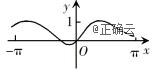
\includegraphics[width=.42\linewidth]{assets/asset-093-01.jpg}
\end{center}
\begin{choices}
  \item A． (图片)
  \item B． (图片)
  \item C． (图片)
  \item D． (图片)
\end{choices}
\begin{solution}
\textbf{答案：}$D$

\textbf{分析：}先判断函数的奇偶性，得 $f(x)$ 是奇函数，排除 $A$，再注意到选项的区别，利用特殊值得正确答案．

\textbf{详解：}由 $f(-x) = \frac{\sin(-x) + (-x)}{\cos(-x) + (-x)^2} = \frac{-\sin x - x}{\cos x + x^2} = -f(x)$，得 $f(x)$ 是奇函数，其图象关于原点对称．又 $f\left(\frac{\pi}{2}\right) = \frac{1 + \frac{\pi}{2}}{\left(\frac{\pi}{2}\right)^2} = \frac{4 + 2\pi}{\pi^2} > 1$, $f(\pi) = \frac{\pi}{-1 + \pi^2} > 0$．故选 $D$．
\end{solution}
\end{question}

\begin{question}[points=5]
\textbf{来源：}2019 年 全国I卷-理科，第 7 题\quad \textbf{专题：}向量\par
已知非零向量 $\mathbf{a}$, $\mathbf{b}$ 满足 $|\mathbf{a}| = 2|\mathbf{b}|$, 且 $(\mathbf{a} - \mathbf{b}) \perp \mathbf{b}$, 则 $\mathbf{a}$ 与 $\mathbf{b}$ 的夹角为
\begin{choices}
  \item $\frac{\pi}{6}$
  \item $\frac{\pi}{3}$
  \item $\frac{2\pi}{3}$
  \item $\frac{5\pi}{6}$
\end{choices}
\begin{solution}
\textbf{答案：}$B$

\textbf{分析：}本题主要考查利用平面向量数量积计算向量长度、夹角与垂直问题，渗透了转化与化归、数学计算等数学素养．先由 $(\mathbf{a} - \mathbf{b}) \perp \mathbf{b}$ 得出向量 $\mathbf{a}$, $\mathbf{b}$ 的数量积与其模的关系，再利用向量夹角公式即可计算出向量夹角．

\textbf{详解：}因为 $(\mathbf{a} - \mathbf{b}) \perp \mathbf{b}$, 所以 $(\mathbf{a} - \mathbf{b}) \cdot \mathbf{b} = \mathbf{a} \cdot \mathbf{b} - |\mathbf{b}|^2 = 0$, 所以 $\mathbf{a} \cdot \mathbf{b} = |\mathbf{b}|^2$, 所以 $\cos \theta = \frac{\mathbf{a} \cdot \mathbf{b}}{|\mathbf{a}| |\mathbf{b}|} = \frac{|\mathbf{b}|^2}{2|\mathbf{b}|^2} = \frac{1}{2}$, 所以 $\mathbf{a}$ 与 $\mathbf{b}$ 的夹角为 $\frac{\pi}{3}$, 故选 $B$．
\end{solution}
\end{question}

\begin{question}[points=5]
\textbf{来源：}2019 年 全国I卷-理科，第 11 题\quad \textbf{专题：}三角函数\par
关于函数 $f(x) = \sin|x| + |\sin x|$ 有下述四个结论：

① $f(x)$ 是偶函数

② $f(x)$ 在区间 $\left(\frac{\pi}{2}, \pi\right)$ 单调递增

③ $f(x)$ 在 $[-\pi, \pi]$ 有 $4$ 个零点

④ $f(x)$ 的最大值为 $2$

其中所有正确结论的编号是
\begin{choices}
  \item ①②④
  \item ②④
  \item ①④
  \item ①③
\end{choices}
\begin{solution}
\textbf{答案：}$C$

\textbf{分析：}画出函数 $f(x) = \sin|x| + |\sin x|$ 的图象，由图象可得①④正确，故选 $C$．

\textbf{详解：}$\because f(-x) = \sin|-x| + |\sin(-x)| = \sin|x| + |\sin x| = f(x)$, $\therefore f(x)$ 为偶函数，故①正确．当 $\frac{\pi}{2} < x < \pi$ 时，$f(x) = 2\sin x$，它在区间 $\left(\frac{\pi}{2}, \pi\right)$ 单调递减，故②错误．当 $0 \le x \le \pi$ 时，$f(x) = 2\sin x$，它有两个零点：$0$, $\pi$；当 $-\pi \le x < 0$ 时，$f(x) = \sin(-x) - \sin x = -2\sin x$，它有一个零点：$-\pi$，故 $f(x)$ 在 $[-\pi, \pi]$ 有 $3$ 个零点：$-\pi$, $0$, $\pi$，故③错误．当 $x \in [2k\pi, 2k\pi + \pi] (k \in \mathbb{N}^*)$ 时，$f(x) = 2\sin x$；当 $x \in [2k\pi + \pi, 2k\pi + 2\pi] (k \in \mathbb{N}^*)$ 时，$f(x) = \sin x - \sin x = 0$，又 $f(x)$ 为偶函数，$\therefore f(x)$ 的最大值为 $2$，故④正确．综上所述，①④正确，故选 $C$．
\end{solution}
\end{question}

\begin{question}[points=5]
\textbf{来源：}2019 年 全国I卷-理科，第 16 题\quad \textbf{专题：}向量\par
已知双曲线 $C$：$\frac{x^2}{a^2} - \frac{y^2}{b^2} = 1$ $(a > 0, b > 0)$ 的左、右焦点分别为 $F_1$, $F_2$，过 $F_1$ 的直线与 $C$ 的两条渐近线分别交于 $A$, $B$ 两点．若 $\overrightarrow{F_1A} = \overrightarrow{AB}$, $\overrightarrow{F_1B} \cdot \overrightarrow{F_2B} = 0$，则 $C$ 的离心率为．
\fillin[{$2$}]
\begin{solution}
\textbf{答案：}$2$

\textbf{分析：}本题考查平面向量结合双曲线的渐进线和离心率，渗透了逻辑推理、直观想象和数学运算素养．采取几何法，利用数形结合思想解题．

\textbf{详解：}如图，由 $\overrightarrow{F_1A} = \overrightarrow{AB}$, 得 $|F_1A| = |AB|$. 又 $|OF_1| = |OF_2|$, 得 $OA$ 是三角形 $F_1F_2B$ 的中位线，即 $BF_2 \parallel OA$, $|BF_2| = 2|OA|$. 由 $\overrightarrow{F_1B} \cdot \overrightarrow{F_2B} = 0$, 得 $F_1B \perp F_2B$, $OA \perp F_1A$, 则 $|OB| = |OF_1| = |OF_2|$, 有 $\angle OBF_2 = \angle BF_2O = 2\angle OBF_1 = 2\angle OF_1B$, $\angle AOB = \angle AOF_1$. 又 $OA$ 与 $OB$ 都是渐近线，得 $\angle BOF_2 = \angle AOF_1$, 则 $\angle BOF_2 = 60^\circ$. 又渐近线 $OB$ 的斜率为 $\frac{b}{a} = \tan 60^\circ = \sqrt{3}$, 所以该双曲线的离心率为 $e = \frac{c}{a} = \sqrt{1 + \left(\frac{b}{a}\right)^2} = \sqrt{1 + (\sqrt{3})^2} = 2$．
\end{solution}
\end{question}

\begin{question}[points=12]
\textbf{来源：}2019 年 全国I卷-理科，第 17 题\quad \textbf{专题：}三角形、三角函数\par
$\triangle ABC$ 的内角 $A$, $B$, $C$ 的对边分别为 $a$, $b$, $c$, 设 $(\sin B - \sin C)^2 = \sin^2 A - \sin B \sin C$．

(1) 求 $A$;

(2) 若 $\sqrt{2}a + b = 2c$, 求 $\sin C$．
\begin{solution}
\textbf{答案：}(1) $A = \frac{\pi}{3}$; (2) $\sin C = \frac{\sqrt{6} + \sqrt{2}}{4}$

\textbf{分析：}(1) 利用正弦定理化简已知边角关系式可得：$b^2 + c^2 - a^2 = bc$，从而可整理出 $\cos A$，根据 $A \in (0, \pi)$ 可求得结果；(2) 利用正弦定理可得 $\sqrt{2}\sin A + \sin B = 2\sin C$，利用 $\sin B = \sin(A + C)$、两角和差正弦公式可得关于 $\sin C$ 和 $\cos C$ 的方程，结合同角三角函数关系解方程可求得结果．

\textbf{详解：}(1) $(\sin B - \sin C)^2 = \sin^2 B - 2\sin B\sin C + \sin^2 C = \sin^2 A - \sin B\sin C$，即 $\sin^2 B + \sin^2 C - \sin^2 A = \sin B\sin C$，由正弦定理可得：$b^2 + c^2 - a^2 = bc$，$\therefore \cos A = \frac{b^2 + c^2 - a^2}{2bc} = \frac{1}{2}$，$\because A \in (0, \pi)$，$\therefore A = \frac{\pi}{3}$．
(2) $\because \sqrt{2}a + b = 2c$，由正弦定理得：$\sqrt{2}\sin A + \sin B = 2\sin C$，又 $\sin B = \sin(A + C) = \sin A \cos C + \cos A \sin C$，$A = \frac{\pi}{3}$，$\therefore \sqrt{2} \times \frac{\sqrt{3}}{2} + \frac{\sqrt{3}}{2}\cos C + \frac{1}{2}\sin C = 2\sin C$，整理可得：$3\sin C - \sqrt{6} = 3\cos C$，$\because \sin^2 C + \cos^2 C = 1$，$\therefore (3\sin C - \sqrt{6})^2 = 9(1 - \sin^2 C)$，解得：$\sin C = \frac{\sqrt{6} + \sqrt{2}}{4}$ 或 $\frac{\sqrt{6} - \sqrt{2}}{4}$．因为 $\sin B = 2\sin C - \sqrt{2}\sin A = 2\sin C - \frac{\sqrt{6}}{2} > 0$，所以 $\sin C > \frac{\sqrt{6}}{4}$，故 $\sin C = \frac{\sqrt{6} + \sqrt{2}}{4}$．
\end{solution}
\end{question}

\begin{question}[points=12]
\textbf{来源：}2019 年 全国I卷-理科，第 19 题\quad \textbf{专题：}向量\par
已知抛物线 $C$：$y^2 = 3x$ 的焦点为 $F$，斜率为 $\frac{3}{2}$ 的直线 $l$ 与 $C$ 的交点为 $A$, $B$，与 $x$ 轴的交点为 $P$．

(1) 若 $|AF| + |BF| = 4$，求 $l$ 的方程；

(2) 若 $\overrightarrow{AP} = 3\overrightarrow{PB}$，求 $|AB|$．
\begin{solution}
\textbf{答案：}(1) $12x - 8y - 7 = 0$; (2) $\frac{4\sqrt{13}}{3}$

\textbf{分析：}(1) 设直线 $l$：$y = \frac{3}{2}x + m$，$A(x_1, y_1)$, $B(x_2, y_2)$；根据抛物线焦半径公式可得 $x_1 + x_2 = 1$；联立直线方程与抛物线方程，利用韦达定理可构造关于 $m$ 的方程，解方程求得结果；(2) 设直线 $l$：$x = \frac{2}{3}y + t$；联立直线方程与抛物线方程，得到韦达定理的形式；利用 $\overrightarrow{AP} = 3\overrightarrow{PB}$ 可得 $y_1 = -3y_2$，结合韦达定理可求得 $y_1y_2$；根据弦长公式可求得结果．

\textbf{详解：}(1) 设直线 $l$ 方程为：$y = \frac{3}{2}x + m$, $A(x_1, y_1)$, $B(x_2, y_2)$．由抛物线焦半径公式可知：$|AF| + |BF| = x_1 + x_2 + \frac{3}{2} = 4$，$\therefore x_1 + x_2 = \frac{5}{2}$．联立 $\begin{cases} y = \frac{3}{2}x + m \\ y^2 = 3x \end{cases}$ 得：$9x^2 + (12m - 12)x + 4m^2 = 0$，则 $\Delta = (12m - 12)^2 - 144m^2 > 0$，$\therefore m < \frac{1}{2}$，$\therefore x_1 + x_2 = -\frac{12m - 12}{9} = \frac{5}{2}$，解得：$m = -\frac{7}{8}$．$\therefore$ 直线 $l$ 的方程为：$y = \frac{3}{2}x - \frac{7}{8}$，即 $12x - 8y - 7 = 0$．
(2) 设 $P(t, 0)$，则可设直线 $l$ 方程为：$x = \frac{2}{3}y + t$．联立 $\begin{cases} x = \frac{2}{3}y + t \\ y^2 = 3x \end{cases}$ 得：$y^2 - 2y - 3t = 0$，则 $\Delta = 4 + 12t > 0$，$\therefore t > -\frac{1}{3}$，$\therefore y_1 + y_2 = 2$, $y_1y_2 = -3t$．$\because \overrightarrow{AP} = 3\overrightarrow{PB}$，$\therefore y_1 = -3y_2$，$\therefore y_2 = -1$, $y_1 = 3$，$\therefore y_1y_2 = -3$．则 $|AB| = \sqrt{1 + \frac{4}{9}} \cdot \sqrt{(y_1 + y_2)^2 - 4y_1y_2} = \frac{\sqrt{13}}{3} \cdot \sqrt{4 + 12} = \frac{4\sqrt{13}}{3}$．
\end{solution}
\end{question}

\begin{question}[points=12]
\textbf{来源：}2019 年 全国I卷-理科，第 20 题\quad \textbf{专题：}三角函数\par
已知函数 $f(x) = \sin x - \ln(1 + x)$, $f'(x)$ 为 $f(x)$ 的导数．证明：

(1) $f'(x)$ 在区间 $\left(-1, \frac{\pi}{2}\right)$ 存在唯一极大值点；

(2) $f(x)$ 有且仅有 $2$ 个零点．
\begin{solution}
\textbf{答案：}见解析

\textbf{分析：}(1) 求得导函数后，可判断出导函数在 $\left(-1, \frac{\pi}{2}\right)$ 上单调递减，根据零点存在定理可判断出 $\exists x_0 \in \left(0, \frac{\pi}{2}\right)$，使得 $g'(x_0) = 0$，进而得到导函数在 $\left(-1, \frac{\pi}{2}\right)$ 上的单调性，从而可证得结论；(2) 由（1）的结论可知 $x = 0$ 为 $f(x)$ 在 $(-1, 0]$ 上的唯一零点；当 $x \in \left(0, \frac{\pi}{2}\right]$ 时，首先可判断出在 $(0, x_0)$ 上无零点，再利用零点存在定理得到 $f(x)$ 在 $\left(x_0, \frac{\pi}{2}\right)$ 上的单调性，可知 $f(x) > 0$，不存在零点；当 $x \in \left[\frac{\pi}{2}, \pi\right]$ 时，利用零点存在定理和 $f(x)$ 单调性可判断出存在唯一一个零点；当 $x \in (\pi, +\infty)$，可证得 $f(x) < 0$；综合上述情况可证得结论．

\textbf{详解：}(1) 由题意知：$f(x)$ 定义域为 $(-1, +\infty)$ 且 $f'(x) = \cos x - \frac{1}{x+1}$．令 $g(x) = \cos x - \frac{1}{x+1}$, $x \in \left(-1, \frac{\pi}{2}\right)$，$\therefore g'(x) = -\sin x + \frac{1}{(x+1)^2}$, $x \in \left(-1, \frac{\pi}{2}\right)$．$\because \frac{1}{(x+1)^2}$ 在 $\left(-1, \frac{\pi}{2}\right)$ 上单调递减，$-\sin x$ 在 $\left(-1, \frac{\pi}{2}\right)$ 上单调递减，$\therefore g'(x)$ 在 $\left(-1, \frac{\pi}{2}\right)$ 上单调递减．又 $g'(0) = -\sin 0 + 1 = 1 > 0$, $g'\left(\frac{\pi}{2}\right) = -\sin\frac{\pi}{2} + \frac{4}{(\pi+2)^2} = -1 + \frac{4}{(\pi+2)^2} < 0$，$\therefore \exists x_0 \in \left(0, \frac{\pi}{2}\right)$，使得 $g'(x_0) = 0$．$\therefore$ 当 $x \in (-1, x_0)$ 时，$g'(x) > 0$；当 $x \in \left(x_0, \frac{\pi}{2}\right)$ 时，$g'(x) < 0$．即 $g(x)$ 在 $(-1, x_0)$ 上单调递增；在 $\left(x_0, \frac{\pi}{2}\right)$ 上单调递减，则 $x = x_0$ 为 $g(x)$ 唯一的极大值点，即 $f'(x)$ 在区间 $\left(-1, \frac{\pi}{2}\right)$ 上存在唯一的极大值点 $x_0$．
(2) 由（1）知：$f'(x) = \cos x - \frac{1}{x+1}$, $x \in (-1, +\infty)$．
①当 $x \in (-1, 0]$ 时，由（1）可知 $f'(x)$ 在 $(-1, 0]$ 上单调递增，$\therefore f'(x) \le f'(0) = 0$，$\therefore f(x)$ 在 $(-1, 0]$ 上单调递减，又 $f(0) = 0$，$\therefore x = 0$ 为 $f(x)$ 在 $(-1, 0]$ 上的唯一零点．
②当 $x \in \left(0, \frac{\pi}{2}\right]$ 时，$f'(x)$ 在 $(0, x_0)$ 上单调递增，在 $\left(x_0, \frac{\pi}{2}\right)$ 上单调递减，又 $f'(0) = 0$，$\therefore f'(x_0) > 0$，$\therefore f(x)$ 在 $(0, x_0)$ 上单调递增，此时 $f(x) > f(0) = 0$，不存在零点．又 $f'\left(\frac{\pi}{2}\right) = \cos\frac{\pi}{2} - \frac{2}{\pi+2} = -\frac{2}{\pi+2} < 0$，$\therefore \exists x_1 \in \left(x_0, \frac{\pi}{2}\right)$，使得 $f'(x_1) = 0$，$\therefore f(x)$ 在 $(x_0, x_1)$ 上单调递增，在 $\left(x_1, \frac{\pi}{2}\right)$ 上单调递减．又 $f(x_0) > f(0) = 0$, $f\left(\frac{\pi}{2}\right) = \sin\frac{\pi}{2} - \ln\left(1 + \frac{\pi}{2}\right) = \ln\frac{2e}{\pi+2} > \ln 1 = 0$，$\therefore f(x) > 0$ 在 $\left(x_0, \frac{\pi}{2}\right)$ 上恒成立，此时不存在零点．
③当 $x \in \left[\frac{\pi}{2}, \pi\right]$ 时，$\sin x$ 单调递减，$-\ln(x+1)$ 单调递减，$\therefore f(x)$ 在 $\left[\frac{\pi}{2}, \pi\right]$ 上单调递减．又 $f\left(\frac{\pi}{2}\right) > 0$, $f(\pi) = \sin\pi - \ln(\pi+1) = -\ln(\pi+1) < 0$，即 $f(\pi) \cdot f\left(\frac{\pi}{2}\right) < 0$，又 $f(x)$ 在 $\left[\frac{\pi}{2}, \pi\right]$ 上单调递减，$\therefore f(x)$ 在 $\left[\frac{\pi}{2}, \pi\right]$ 上存在唯一零点．
④当 $x \in (\pi, +\infty)$ 时，$\sin x \in [-1, 1]$, $\ln(x+1) > \ln(\pi+1) > \ln e = 1$，$\therefore \sin x - \ln(x+1) < 0$，即 $f(x)$ 在 $(\pi, +\infty)$ 上不存在零点．
综上所述：$f(x)$ 有且仅有 $2$ 个零点．
\end{solution}
\end{question}

\begin{question}[points=5]
\textbf{来源：}2019 年 全国I卷-文科，第 5 题\quad \textbf{专题：}三角函数\par
函数 $f(x)=\frac{\sin x + x}{\cos x + x^2}$ 在 $[-\pi,\pi]$ 的图像大致为
\begin{choices}
  \item A
  \item B
  \item C
  \item D
\end{choices}
\begin{solution}
\textbf{答案：}D

\textbf{分析：}先判断函数的奇偶性，得 $f(x)$ 是奇函数，排除 A，再注意到选项的区别，利用特殊值得正确答案。

\textbf{详解：}由 $f(-x)=\frac{\sin(-x)+(-x)}{\cos(-x)+(-x)^2} = \frac{-\sin x - x}{\cos x + x^2} = -f(x)$，得 $f(x)$ 是奇函数，其图象关于原点对称．又 $f(\frac{\pi}{2}) = \frac{1+\frac{\pi}{2}}{(\frac{\pi}{2})^2} = \frac{4+2\pi}{\pi^2} > 1$，$f(\pi) = \frac{\pi}{-1+\pi^2} > 0$。故选 D。
\end{solution}
\end{question}

\begin{question}[points=5]
\textbf{来源：}2019 年 全国I卷-文科，第 7 题\quad \textbf{专题：}三角函数\par
$\tan 255° =$
\begin{choices}
  \item $-2-\sqrt{3}$
  \item $-2+\sqrt{3}$
  \item $2-\sqrt{3}$
  \item $2+\sqrt{3}$
\end{choices}
\begin{solution}
\textbf{答案：}D

\textbf{分析：}本题首先应用诱导公式，将问题转化成锐角三角函数的计算，进一步应用两角和的正切公式计算求解。

\textbf{详解：}$\tan 255° = \tan(180°+75°) = \tan 75° = \tan(45°+30°) = \frac{\tan 45°+\tan 30°}{1-\tan 45°\tan 30°} = \frac{1+\frac{\sqrt{3}}{3}}{1-\frac{\sqrt{3}}{3}} = 2+\sqrt{3}$。
\end{solution}
\end{question}

\begin{question}[points=5]
\textbf{来源：}2019 年 全国I卷-文科，第 8 题\quad \textbf{专题：}向量\par
已知非零向量 $\boldsymbol{a}$，$\boldsymbol{b}$ 满足 $|\boldsymbol{a}|=2|\boldsymbol{b}|$，且 $(\boldsymbol{a}-\boldsymbol{b}) \perp \boldsymbol{b}$，则 $\boldsymbol{a}$ 与 $\boldsymbol{b}$ 的夹角为
\begin{choices}
  \item $\frac{\pi}{6}$
  \item $\frac{\pi}{3}$
  \item $\frac{2\pi}{3}$
  \item $\frac{5\pi}{6}$
\end{choices}
\begin{solution}
\textbf{答案：}B

\textbf{分析：}本题主要考查利用平面向量数量积计算向量长度、夹角与垂直问题，先由 $(\boldsymbol{a}-\boldsymbol{b}) \perp \boldsymbol{b}$ 得出向量 $\boldsymbol{a},\boldsymbol{b}$ 的数量积与其模的关系，再利用向量夹角公式即可计算出向量夹角。

\textbf{详解：}因为 $(\boldsymbol{a}-\boldsymbol{b}) \perp \boldsymbol{b}$，所以 $(\boldsymbol{a}-\boldsymbol{b})\cdot\boldsymbol{b} = \boldsymbol{a}\cdot\boldsymbol{b} - |\boldsymbol{b}|^2 = 0$，所以 $\boldsymbol{a}\cdot\boldsymbol{b} = |\boldsymbol{b}|^2$，所以 $\cos\theta = \frac{\boldsymbol{a}\cdot\boldsymbol{b}}{|\boldsymbol{a}||\boldsymbol{b}|} = \frac{|\boldsymbol{b}|^2}{2|\boldsymbol{b}|^2} = \frac{1}{2}$，所以 $\boldsymbol{a}$ 与 $\boldsymbol{b}$ 的夹角为 $\frac{\pi}{3}$，故选 B。
\end{solution}
\end{question}

\begin{question}[points=5]
\textbf{来源：}2019 年 全国I卷-文科，第 10 题\quad \textbf{专题：}三角函数\par
双曲线 $C: \frac{x^2}{a^2} - \frac{y^2}{b^2} = 1$ ($a>0,b>0$) 的一条渐近线的倾斜角为 130°，则 $C$ 的离心率为
\begin{choices}
  \item $2\sin40°$
  \item $2\cos40°$
  \item $\frac{1}{\sin50°}$
  \item $\frac{1}{\cos50°}$
\end{choices}
\begin{solution}
\textbf{答案：}D

\textbf{分析：}由双曲线渐近线定义可得 $-\frac{b}{a} = \tan130°$，$\Rightarrow \frac{b}{a} = \tan50°$，再利用 $e = \frac{c}{a} = \sqrt{1+\left(\frac{b}{a}\right)^2}$ 求双曲线的离心率。

\textbf{详解：}由已知可得 $-\frac{b}{a} = \tan130°$，$\Rightarrow \frac{b}{a} = \tan50°$，$\Rightarrow e = \frac{c}{a} = \sqrt{1+\left(\frac{b}{a}\right)^2} = \sqrt{1+\tan^2 50°} = \sqrt{1+\frac{\sin^2 50°}{\cos^2 50°}} = \sqrt{\frac{\sin^2 50°+\cos^2 50°}{\cos^2 50°}} = \frac{1}{\cos50°}$，故选 D。
\end{solution}
\end{question}

\begin{question}[points=5]
\textbf{来源：}2019 年 全国I卷-文科，第 11 题\quad \textbf{专题：}三角形、三角函数\par
$\triangle ABC$ 的内角 $A$，$B$，$C$ 的对边分别为 $a$，$b$，$c$，已知 $a\sin A - b\sin B = 4c\sin C$，$\cos A = -\frac{1}{4}$，则 $\frac{b}{c} =$
\begin{choices}
  \item 6
  \item 5
  \item 4
  \item 3
\end{choices}
\begin{solution}
\textbf{答案：}A

\textbf{分析：}利用正弦定理和余弦定理推论得出 $a$，$b$，$c$ 关系，列出方程解出结果。

\textbf{详解：}由已知及正弦定理可得 $a^2 - b^2 = 4c^2$，由余弦定理推论可得 $-\frac{1}{4} = \cos A = \frac{b^2+c^2-a^2}{2bc}$，$\Rightarrow \frac{c^2-4c^2}{2bc} = -\frac{1}{4}$，$\Rightarrow \frac{3c}{2b} = \frac{1}{4}$，$\Rightarrow \frac{b}{c} = \frac{3}{2} \times 4 = 6$，故选 A。
\end{solution}
\end{question}

\begin{question}[points=5]
\textbf{来源：}2019 年 全国I卷-文科，第 15 题\quad \textbf{专题：}三角函数\par
函数 $f(x) = \sin(2x+\frac{3\pi}{2}) - 3\cos x$ 的最小值为．
\fillin[{$-4$}]
\begin{solution}
\textbf{答案：}$-4$

\textbf{分析：}本题首先应用诱导公式，转化得到二倍角的余弦，进一步应用二倍角的余弦公式，得到关于 $\cos x$ 的二次函数。

\textbf{详解：}$f(x) = \sin(2x+\frac{3\pi}{2}) - 3\cos x = -\cos 2x - 3\cos x = -2\cos^2 x - 3\cos x + 1 = -2(\cos x + \frac{3}{4})^2 + \frac{17}{8}$，因为 $-1 \le \cos x \le 1$，所以当 $\cos x = 1$ 时，$f_{\min}(x) = -4$，故函数 $f(x)$ 的最小值为 $-4$。
\end{solution}
\end{question}

\begin{question}[points=12]
\textbf{来源：}2019 年 全国I卷-文科，第 20 题\quad \textbf{专题：}三角函数\par
已知函数 $f(x) = 2\sin x - x\cos x - x$，$f'(x)$ 为 $f(x)$ 的导数．

（1）证明：$f'(x)$ 在区间 $(0,\pi)$ 存在唯一零点；

（2）若 $x \in [0,\pi]$ 时，$f(x) \ge ax$，求 $a$ 的取值范围．
\begin{solution}
\textbf{答案：}（1）见解析；（2）$a \in (-\infty, 0]$。

\textbf{分析：}（1）求导得到导函数后，设为 $g(x)$ 进行再次求导，可判断出当 $x \in (0,\frac{\pi}{2})$ 时 $g'(x)>0$，当 $x \in (\frac{\pi}{2},\pi)$ 时 $g'(x)<0$，从而得到 $g(x)$ 单调性，由零点存在定理可判断出唯一零点；（2）构造函数 $h(x)=f(x)-ax$，通过二次求导可判断出 $h'(x)$ 的最值，分别在 $a \le -2$，$-2<a\le0$，$0<a<\frac{\pi-2}{2}$ 和 $a \ge \frac{\pi-2}{2}$ 的情况下根据导函数的符号判断 $h(x)$ 单调性，从而确定 $h(x)\ge0$ 恒成立时 $a$ 的取值范围。

\textbf{详解：}（1）$f'(x)=2\cos x - \cos x + x\sin x -1 = \cos x + x\sin x -1$，令 $g(x)=\cos x + x\sin x -1$，则 $g'(x)=-\sin x + \sin x + x\cos x = x\cos x$．当 $x \in (0,\pi)$ 时，令 $g'(x)=0$，解得 $x=\frac{\pi}{2}$，当 $x\in(0,\frac{\pi}{2})$ 时 $g'(x)>0$；当 $x\in(\frac{\pi}{2},\pi)$ 时 $g'(x)<0$，所以 $g(x)$ 在 $(0,\frac{\pi}{2})$ 上单调递增，在 $(\frac{\pi}{2},\pi)$ 上单调递减．又 $g(0)=1-1=0$，$g(\frac{\pi}{2})=\frac{\pi}{2}-1>0$，$g(\pi)=-1-1=-2$，所以 $g(x)$ 在 $(0,\frac{\pi}{2})$ 无零点，在 $(\frac{\pi}{2},\pi)$ 存在唯一零点，即 $f'(x)$ 在 $(0,\pi)$ 存在唯一零点。
（2）若 $x\in[0,\pi]$ 时，$f(x)\ge ax$，即 $f(x)-ax\ge0$ 恒成立，令 $h(x)=f(x)-ax=2\sin x - x\cos x - (a+1)x$，则 $h'(x)=\cos x + x\sin x -1 - a$，$h''(x)=x\cos x = g'(x)$．由（1）可知，$h'(x)$ 在 $(0,\frac{\pi}{2})$ 上单调递增，在 $(\frac{\pi}{2},\pi)$ 上单调递减，且 $h'(0)=-a$，$h'(\frac{\pi}{2})=\frac{\pi-2}{2}-a$，$h'(\pi)=-2-a$，所以 $h'(x)_{\min}=h'(\pi)=-2-a$，$h'(x)_{\max}=h'(\frac{\pi}{2})=\frac{\pi-2}{2}-a$．
①当 $a\le -2$ 时，$h'(x)_{\min}=-2-a\ge0$，即 $h'(x)\ge0$ 在 $[0,\pi]$ 上恒成立，$h(x)$ 单调递增，$h(x)\ge h(0)=0$，恒成立；
②当 $-2<a\le0$ 时，$h'(0)\ge0$，$h'(\frac{\pi}{2})>0$，$h'(\pi)<0$，$\exists x_1\in(\frac{\pi}{2},\pi)$ 使得 $h'(x_1)=0$，$h(x)$ 在 $[0,x_1)$ 单调递增，在 $(x_1,\pi]$ 单调递减，又 $h(0)=0$，$h(\pi)=2\sin \pi - \pi\cos \pi - (a+1)\pi = -a\pi \ge 0$，所以恒成立；
③当 $0<a<\frac{\pi-2}{2}$ 时，$h'(0)<0$，$h'(\frac{\pi}{2})>0$，$\exists x_2\in(0,\frac{\pi}{2})$ 使得 $h'(x_2)=0$，$h(x)$ 在 $[0,x_2)$ 单调递减，在 $(x_2,\frac{\pi}{2})$ 单调递增，则 $x\in(0,x_2)$ 时 $h(x)<h(0)=0$，不恒成立；
④当 $a\ge \frac{\pi-2}{2}$ 时，$h'(x)_{\max}=h'(\frac{\pi}{2})=\frac{\pi-2}{2}-a\le0$，$h(x)$ 在 $(0,\frac{\pi}{2})$ 单调递减，$h(x)<h(0)=0$，不恒成立．
综上所述：$a\in(-\infty,0]$。
\end{solution}
\end{question}

\section*{2020 年}

\begin{question}[points=5]
\textbf{来源：}2020 年 全国III卷-理科，第 6 题\quad \textbf{专题：}向量、三角函数\par
已知向量 $\mathbf{a},\mathbf{b}$ 满足 $|\mathbf{a}|=5$，$|\mathbf{b}|=6$，$\mathbf{a}\cdot\mathbf{b}=-6$，则 $\cos\langle\mathbf{a},\mathbf{a}+\mathbf{b}\rangle=$
\begin{choices}
  \item $-\dfrac{31}{35}$
  \item $-\dfrac{19}{35}$
  \item $\dfrac{17}{35}$
  \item $\dfrac{19}{35}$
\end{choices}
\begin{solution}
\textbf{答案：}$D$

\textbf{分析：}计算出 $\mathbf{a}\cdot(\mathbf{a}+\mathbf{b})$ 和 $|\mathbf{a}+\mathbf{b}|$ 的值，利用平面向量数量积公式计算。

\textbf{详解：}因为 $|\mathbf{a}|=5$，$|\mathbf{b}|=6$，$\mathbf{a}\cdot\mathbf{b}=-6$，所以 $\mathbf{a}\cdot(\mathbf{a}+\mathbf{b})=|\mathbf{a}|^2+\mathbf{a}\cdot\mathbf{b}=25-6=19$。$|\mathbf{a}+\mathbf{b}|=\sqrt{|\mathbf{a}|^2+2\mathbf{a}\cdot\mathbf{b}+|\mathbf{b}|^2}=\sqrt{25-12+36}=7$。因此 $\cos\langle\mathbf{a},\mathbf{a}+\mathbf{b}\rangle=\dfrac{\mathbf{a}\cdot(\mathbf{a}+\mathbf{b})}{|\mathbf{a}||\mathbf{a}+\mathbf{b}|}=\dfrac{19}{5\times7}=\dfrac{19}{35}$。故选 $D$。
\end{solution}
\end{question}

\begin{question}[points=5]
\textbf{来源：}2020 年 全国III卷-理科，第 7 题\quad \textbf{专题：}三角形、三角函数\par
在 $\triangle ABC$ 中，$\cos C=\dfrac{2}{3}$，$AC=4$，$BC=3$，则 $\cos B=$
\begin{choices}
  \item $\dfrac{1}{9}$
  \item $\dfrac{1}{3}$
  \item $\dfrac{1}{2}$
  \item $\dfrac{2}{3}$
\end{choices}
\begin{solution}
\textbf{答案：}$A$

\textbf{分析：}利用余弦定理先求 $AB$，再利用余弦定理求 $\cos B$。

\textbf{详解：}由余弦定理 $AB^2=AC^2+BC^2-2\cdot AC\cdot BC\cdot\cos C=4^2+3^2-2\times4\times3\times\dfrac{2}{3}=16+9-16=9$，所以 $AB=3$。再由余弦定理 $\cos B=\dfrac{AB^2+BC^2-AC^2}{2\cdot AB\cdot BC}=\dfrac{9+9-16}{2\times3\times3}=\dfrac{2}{18}=\dfrac{1}{9}$。故选 $A$。
\end{solution}
\end{question}

\begin{question}[points=5]
\textbf{来源：}2020 年 全国III卷-理科，第 9 题\quad \textbf{专题：}三角函数\par
已知 $2\tan\theta-\tan\left(\theta+\dfrac{\pi}{4}\right)=7$，则 $\tan\theta=$
\begin{choices}
  \item $-2$
  \item $-1$
  \item $1$
  \item $2$
\end{choices}
\begin{solution}
\textbf{答案：}$D$

\textbf{分析：}利用两角和的正切公式，结合换元法解一元二次方程。

\textbf{详解：}由 $2\tan\theta-\tan(\theta+\frac{\pi}{4})=7$，得 $2\tan\theta-\dfrac{\tan\theta+1}{1-\tan\theta}=7$。令 $t=\tan\theta$，$t\neq1$，则 $2t-\dfrac{t+1}{1-t}=7$，整理得 $t^2-4t+4=0$，解得 $t=2$。所以 $\tan\theta=2$。故选 $D$。
\end{solution}
\end{question}

\begin{question}[points=5]
\textbf{来源：}2020 年 全国III卷-理科，第 16 题\quad \textbf{专题：}三角函数\par
关于函数 $f(x)=\sin x+\dfrac{1}{\sin x}$ 有如下四个命题：

① $f(x)$ 的图像关于 $y$ 轴对称。

② $f(x)$ 的图像关于原点对称。

③ $f(x)$ 的图像关于直线 $x=\dfrac{\pi}{2}$ 对称。

④ $f(x)$ 的最小值为 $2$。

其中所有真命题的序号是 。
\fillin[{$②③$}]
\begin{solution}
\textbf{答案：}$②③$

\textbf{分析：}利用特殊值法、函数奇偶性定义、对称性定义及取特殊值判断。

\textbf{详解：}因为 $f\left(\frac{\pi}{6}\right)=\frac12+2=\frac52$，$f\left(-\frac{\pi}{6}\right)=-\frac12-2=-\frac52$，不相等，所以①错误。定义域为 $\{x|x\neq k\pi,k\in\mathbb{Z}\}$，关于原点对称，$f(-x)=\sin(-x)+\frac{1}{\sin(-x)}=-\sin x-\frac{1}{\sin x}=-f(x)$，所以②正确。因为 $f\left(\frac{\pi}{2}-x\right)=\cos x+\frac{1}{\cos x}=f\left(\frac{\pi}{2}+x\right)$，所以③正确。当 $-\pi<x<0$ 时，$\sin x<0$，$f(x)=\sin x+\frac{1}{\sin x}<0<2$，所以④错误。故真命题序号为②③。
\end{solution}
\end{question}

\begin{question}[points=5]
\textbf{来源：}2020 年 全国III卷-文科，第 5 题\quad \textbf{专题：}三角函数\par
已知 $\sin\theta+\sin(\theta+\frac{\pi}{3})=1$，则 $\sin(\theta+\frac{\pi}{6})=$
\begin{choices}
  \item $\frac{1}{2}$
  \item $\frac{\sqrt{3}}{3}$
  \item $\frac{\sqrt{2}}{3}$
  \item $\frac{\sqrt{2}}{2}$
\end{choices}
\begin{solution}
\textbf{答案：}B

\textbf{分析：}将所给的三角函数式展开变形，然后再逆用两角和的正弦公式即可求得三角函数式的值.

\textbf{详解：}由题意可得：$\sin\theta+\frac{1}{2}\sin\theta+\frac{\sqrt{3}}{2}\cos\theta=1$，则 $\frac{3}{2}\sin\theta+\frac{\sqrt{3}}{2}\cos\theta=1$，即 $\frac{\sqrt{3}}{2}\sin\theta+\frac{1}{2}\cos\theta=\frac{\sqrt{3}}{3}$，从而有 $\sin\theta\cos\frac{\pi}{6}+\cos\theta\sin\frac{\pi}{6}=\frac{\sqrt{3}}{3}$，即 $\sin(\theta+\frac{\pi}{6})=\frac{\sqrt{3}}{3}$. 故选：B.
\end{solution}
\end{question}

\begin{question}[points=5]
\textbf{来源：}2020 年 全国III卷-文科，第 6 题\quad \textbf{专题：}向量\par
在平面内，$A$，$B$ 是两个定点，$C$ 是动点，若 $\overrightarrow{AC}\cdot\overrightarrow{BC}=1$，则点 $C$ 的轨迹为
\begin{choices}
  \item 圆
  \item 椭圆
  \item 抛物线
  \item 直线
\end{choices}
\begin{solution}
\textbf{答案：}A

\textbf{分析：}首先建立平面直角坐标系，然后结合数量积的定义求解其轨迹方程即可.

\textbf{详解：}设 $|AB|=2a\ (a>0)$，以 $AB$ 中点为坐标原点建立平面直角坐标系，则 $A(-a,0),B(a,0)$，设 $C(x,y)$，可得 $\overrightarrow{AC}=(x+a,y),\overrightarrow{BC}=(x-a,y)$，从而 $\overrightarrow{AC}\cdot\overrightarrow{BC}=(x+a)(x-a)+y^2$，结合题意得 $(x+a)(x-a)+y^2=1$，整理得 $x^2+y^2=a^2+1$，即点 $C$ 的轨迹是以 $AB$ 中点为圆心，$\sqrt{a^2+1}$ 为半径的圆. 故选：A.
\end{solution}
\end{question}

\begin{question}[points=5]
\textbf{来源：}2020 年 全国III卷-文科，第 11 题\quad \textbf{专题：}三角形、三角函数\par
在 $\triangle ABC$ 中，$\cos C=\frac{2}{3}$，$AC=4$，$BC=3$，则 $\tan B=$
\begin{choices}
  \item $\sqrt{5}$
  \item $2\sqrt{5}$
  \item $4\sqrt{5}$
  \item $8\sqrt{5}$
\end{choices}
\begin{solution}
\textbf{答案：}C

\textbf{分析：}先根据余弦定理求 $c$，再根据余弦定理求 $\cos B$，最后根据同角三角函数关系求 $\tan B$.

\textbf{详解：}设 $AB=c, BC=a=3, CA=b=4$，由余弦定理得 $c^2=a^2+b^2-2ab\cos C=9+16-2\times3\times4\times\frac{2}{3}=9$，所以 $c=3$，则 $\cos B=\frac{a^2+c^2-b^2}{2ac}=\frac{9+9-16}{2\times3\times3}=\frac{1}{9}$，$\sin B=\sqrt{1-(\frac{1}{9})^2}=\frac{4\sqrt{5}}{9}$，所以 $\tan B=4\sqrt{5}$. 故选：C.
\end{solution}
\end{question}

\begin{question}[points=5]
\textbf{来源：}2020 年 全国III卷-文科，第 12 题\quad \textbf{专题：}三角函数\par
已知函数 $f(x)=\sin x+\frac{1}{\sin x}$，则
\begin{choices}
  \item $f(x)$ 的最小值为 $2$
  \item $f(x)$ 的图像关于 $y$ 轴对称
  \item $f(x)$ 的图像关于直线 $x=\pi$ 对称
  \item $f(x)$ 的图像关于直线 $x=\frac{\pi}{2}$ 对称
\end{choices}
\begin{solution}
\textbf{答案：}D

\textbf{分析：}根据基本不等式使用条件可判断A；根据奇偶性可判断B；根据对称性判断C,D.

\textbf{详解：}因为 $\sin x$ 可以为负，所以A错；$\sin x\neq0$，$x\neq k\pi(k\in\mathbb Z)$，$f(-x)=-\sin x-\frac{1}{\sin x}=-f(x)$，所以 $f(x)$ 关于原点对称；$f(2\pi-x)=-\sin x-\frac{1}{\sin x}\neq f(x)$，$f(\pi-x)=\sin x+\frac{1}{\sin x}=f(x)$，所以 $f(x)$ 关于直线 $x=\frac{\pi}{2}$ 对称，故C错，D对. 故选：D.
\end{solution}
\end{question}

\begin{question}[points=5]
\textbf{来源：}2020 年 全国II卷-理科，第 2 题\quad \textbf{专题：}三角函数\par
若$\alpha$为第四象限角，则（ ）
\begin{choices}
  \item $\cos2\alpha>0$
  \item $\cos2\alpha<0$
  \item $\sin2\alpha>0$
  \item $\sin2\alpha<0$
\end{choices}
\begin{solution}
\textbf{答案：}$\sin2\alpha<0$

\textbf{分析：}由题意结合二倍角公式确定所给的选项是否正确即可.

\textbf{详解：}当 $\alpha=-\frac{\pi}{6}$ 时，$\cos2\alpha=\cos\left(-\frac{\pi}{3}\right)>0$，选项B错误；当 $\alpha=-\frac{\pi}{3}$ 时，$\cos2\alpha=\cos\left(-\frac{2\pi}{3}\right)<0$，选项A错误；由 $\alpha$ 在第四象限可得：$\sin\alpha<0,\cos\alpha>0$，则 $\sin2\alpha=2\sin\alpha\cos\alpha<0$，选项C错误，选项D正确.
\end{solution}
\end{question}

\begin{question}[points=5]
\textbf{来源：}2020 年 全国II卷-理科，第 13 题\quad \textbf{专题：}向量\par
已知单位向量$\boldsymbol{a},\boldsymbol{b}$的夹角为$45^\circ$，$k\boldsymbol{a}-\boldsymbol{b}$与$\boldsymbol{a}$垂直，则$k=$.
\fillin[{$\dfrac{\sqrt2}{2}$}]
\begin{solution}
\textbf{答案：}$\dfrac{\sqrt2}{2}$

\textbf{分析：}首先求得向量的数量积，然后结合向量垂直的充分必要条件即可求得实数k的值.

\textbf{详解：}由题意可得：$\boldsymbol{a}\cdot\boldsymbol{b}=1\times1\times\cos45^\circ=\dfrac{\sqrt2}{2}$，由向量垂直的充分必要条件可得：$(k\boldsymbol{a}-\boldsymbol{b})\cdot\boldsymbol{a}=0$，即$k\boldsymbol{a}^2-\boldsymbol{a}\cdot\boldsymbol{b}=k-\dfrac{\sqrt2}{2}=0$，解得$k=\dfrac{\sqrt2}{2}$.
\end{solution}
\end{question}

\begin{question}[points=12]
\textbf{来源：}2020 年 全国II卷-理科，第 17 题\quad \textbf{专题：}三角函数\par
$\triangle ABC$中，$\sin^2A-\sin^2B-\sin^2C=\sin B\sin C$.

（1）求$A$；

（2）若$BC=3$，求$\triangle ABC$周长的最大值.
\begin{solution}
\textbf{答案：}（1）$\dfrac{2\pi}{3}$；（2）$3+2\sqrt3$

\textbf{分析：}（1）利用正弦定理角化边，配凑出$\cos A$的形式，进而求得$A$；（2）利用余弦定理可得到$(AC+AB)^2-AC\cdot AB=9$，利用基本不等式可求得$AC+AB$的最大值，进而得到结果.

\textbf{详解：}（1）由正弦定理可得：$BC^2-AC^2-AB^2=AC\cdot AB$，$\therefore\cos A=\dfrac{AC^2+AB^2-BC^2}{2AC\cdot AB}=-\dfrac12$，$\because A\in(0,\pi)$，$\therefore A=\dfrac{2\pi}{3}$.
（2）由余弦定理得：$BC^2=AC^2+AB^2-2AC\cdot AB\cos A=AC^2+AB^2+AC\cdot AB=9$，即$(AC+AB)^2-AC\cdot AB=9$，$\because AC\cdot AB\leq\left(\dfrac{AC+AB}{2}\right)^2$（当且仅当$AC=AB$时取等号），$\therefore9=(AC+AB)^2-AC\cdot AB\geq(AC+AB)^2-\left(\dfrac{AC+AB}{2}\right)^2=\dfrac34(AC+AB)^2$，解得：$AC+AB\leq2\sqrt3$（当且仅当$AC=AB$时取等号），$\therefore\triangle ABC$周长$L=AC+AB+BC\leq3+2\sqrt3$，$\therefore\triangle ABC$周长的最大值为$3+2\sqrt3$.
\end{solution}
\end{question}

\begin{question}[points=12]
\textbf{来源：}2020 年 全国II卷-理科，第 21 题\quad \textbf{专题：}三角函数\par
已知函数$f(x)=\sin^2x\sin2x$.

（1）讨论$f(x)$在区间$(0,\pi)$的单调性；

（2）证明：$|f(x)|\leq\dfrac{3\sqrt3}{8}$；

（3）设$n\in\mathbb{N}^*$，证明：$\sin^2x\sin^22x\sin^24x\cdots\sin^22^nx\leq\dfrac{3^n}{4^n}$.
\begin{solution}
\textbf{答案：}（1）当$x\in(0,\frac\pi3)$时，$f'(x)>0,f(x)$单调递增，当$x\in(\frac\pi3,\frac{2\pi}3)$时，$f'(x)<0,f(x)$单调递减，当$x\in(\frac{2\pi}3,\pi)$时，$f'(x)>0,f(x)$单调递增.（2）证明见解析；（3）证明见解析.

\textbf{分析：}(1)首先求得导函数的解析式，然后由导函数的零点确定其在各个区间上的符号，最后确定原函数的单调性即可；(2)首先确定函数的周期性，然后结合(1)中的结论确定函数在一个周期内的最大值和最小值即可证得题中的不等式；(3)对所给的不等式左侧进行恒等变形，然后结合(2)的结论和三角函数的有界性进行放缩即可证得题中的不等式.

\textbf{详解：}（1）$f(x)=\sin^2x\sin2x=2\sin^3x\cos x$，则$f'(x)=2(3\sin^2x\cos^2x-\sin^4x)=2\sin^2x(3\cos^2x-\sin^2x)=2\sin^2x(4\cos^2x-1)=2\sin^2x(2\cos x+1)(2\cos x-1)$，$f'(x)=0$在$x\in(0,\pi)$上的根为$x_1=\frac\pi3,x_2=\frac{2\pi}3$，当$x\in(0,\frac\pi3)$时，$f'(x)>0,f(x)$单调递增，当$x\in(\frac\pi3,\frac{2\pi}3)$时，$f'(x)<0,f(x)$单调递减，当$x\in(\frac{2\pi}3,\pi)$时，$f'(x)>0,f(x)$单调递增.
（2）注意到$f(x+\pi)=\sin^2(x+\pi)\sin[2(x+\pi)]=\sin^2x\sin2x=f(x)$，故函数$f(x)$是周期为$\pi$的函数，结合(1)的结论，计算可得：$f(0)=f(\pi)=0$，$f(\frac\pi3)=(\frac{\sqrt3}{2})^2\times\frac{\sqrt3}{2}=\frac{3\sqrt3}{8}$，$f(\frac{2\pi}3)=(\frac{\sqrt3}{2})^2\times(-\frac{\sqrt3}{2})=-\frac{3\sqrt3}{8}$，据此可得：$[f(x)]_{\max}=\frac{3\sqrt3}{8}$，$[f(x)]_{\min}=-\frac{3\sqrt3}{8}$，即$|f(x)|\leq\frac{3\sqrt3}{8}$.
（3）$\sin^2x\sin^22x\sin^24x\cdots\sin^22^nx=\left[\sin^3x\sin^32x\sin^34x\cdots\sin^32^nx\right]^{\frac23}=\left[\sin x(\sin^2x\sin2x)(\sin^22x\sin4x)\cdots(\sin^22^{n-1}x\sin2^nx)\sin^22^nx\right]^{\frac23}\leq\left[|\sin x|\times\frac{3\sqrt3}{8}\times\frac{3\sqrt3}{8}\times\cdots\times\frac{3\sqrt3}{8}\times|\sin2^nx|\right]^{\frac23}=\left[\left(\frac{3\sqrt3}{8}\right)^n\right]^{\frac23}=\left(\frac{3}{4}\right)^n$.
\end{solution}
\end{question}

\begin{question}[points=5]
\textbf{来源：}2020 年 全国II卷-文科，第 5 题\quad \textbf{专题：}向量\par
已知单位向量 $\vec{a}$，$\vec{b}$ 的夹角为 $60^\circ$，则在下列向量中，与 $\vec{b}$ 垂直的是（ ）
\begin{choices}
  \item $\vec{a}+2\vec{b}$
  \item $2\vec{a}+\vec{b}$
  \item $\vec{a}-2\vec{b}$
  \item $2\vec{a}-\vec{b}$
\end{choices}
\begin{solution}
\textbf{答案：}D

\textbf{分析：}根据平面向量数量积的定义、运算性质，结合两平面向量垂直数量积为零这一性质逐一判断即可。

\textbf{详解：}由已知可得：$\vec{a}\cdot\vec{b}=|\vec{a}||\vec{b}|\cos60^\circ=1\times1\times\frac{1}{2}=\frac{1}{2}$。
A：$(\vec{a}+2\vec{b})\cdot\vec{b}=\vec{a}\cdot\vec{b}+2|\vec{b}|^2=\frac{1}{2}+2=\frac{5}{2}\neq0$；
B：$(2\vec{a}+\vec{b})\cdot\vec{b}=2\vec{a}\cdot\vec{b}+|\vec{b}|^2=1+1=2\neq0$；
C：$(\vec{a}-2\vec{b})\cdot\vec{b}=\vec{a}\cdot\vec{b}-2|\vec{b}|^2=\frac{1}{2}-2=-\frac{3}{2}\neq0$；
D：$(2\vec{a}-\vec{b})\cdot\vec{b}=2\vec{a}\cdot\vec{b}-|\vec{b}|^2=1-1=0$。
故选：D。
\end{solution}
\end{question}

\begin{question}[points=5]
\textbf{来源：}2020 年 全国II卷-文科，第 13 题\quad \textbf{专题：}三角函数\par
若 $\sin x = -\frac{2}{3}$，则 $\cos 2x = $ ．
\fillin[{$\frac{1}{9}$}]
\begin{solution}
\textbf{答案：}$\frac{1}{9}$

\textbf{分析：}直接利用余弦的二倍角公式进行运算求解。

\textbf{详解：}$\cos 2x = 1-2\sin^2 x = 1-2\times\left(-\frac{2}{3}\right)^2 = 1-\frac{8}{9} = \frac{1}{9}$。
\end{solution}
\end{question}

\begin{question}[points=12]
\textbf{来源：}2020 年 全国II卷-文科，第 17 题\quad \textbf{专题：}三角函数\par
$\triangle ABC$ 的内角 $A,B,C$ 的对边分别为 $a,b,c$，已知 $\cos^2\left(\frac{\pi}{2}+A\right)+\cos A=\frac{5}{4}$。

（1）求 $A$；

（2）若 $b-c=\frac{\sqrt{3}}{3}a$，证明：$\triangle ABC$ 是直角三角形。
\begin{solution}
\textbf{答案：}（1）$A=\frac{\pi}{3}$；（2）证明见解析。

\textbf{分析：}（1）根据诱导公式和同角三角函数平方关系，$\cos^2\left(\frac{\pi}{2}+A\right)+\cos A=\frac{5}{4}$ 可化为 $1-\cos^2 A+\cos A=\frac{5}{4}$，即可解出；
（2）根据余弦定理可得 $b^2+c^2-a^2=bc$，将 $b-c=\frac{\sqrt{3}}{3}a$ 代入可找到 $a,b,c$ 关系，再根据勾股定理或正弦定理即可证出。

\textbf{详解：}（1）因为 $\cos^2\left(\frac{\pi}{2}+A\right)+\cos A=\frac{5}{4}$，所以 $\sin^2 A+\cos A=\frac{5}{4}$，
即 $1-\cos^2 A+\cos A=\frac{5}{4}$，解得 $\cos A=\frac{1}{2}$，又 $0<A<\pi$，所以 $A=\frac{\pi}{3}$。
（2）因为 $A=\frac{\pi}{3}$，所以 $\cos A=\frac{b^2+c^2-a^2}{2bc}=\frac{1}{2}$，即 $b^2+c^2-a^2=bc$①。
又 $b-c=\frac{\sqrt{3}}{3}a$②，将②代入①得，$b^2+c^2-3(b-c)^2=bc$，
即 $2b^2+2c^2-5bc=0$，而 $b>c$，解得 $b=2c$，
所以 $a=\sqrt{3}c$，
故 $b^2=a^2+c^2$，即 $\triangle ABC$ 是直角三角形。
\end{solution}
\end{question}

\begin{question}[points=5]
\textbf{来源：}2020 年 全国I卷-理科，第 7 题\quad \textbf{专题：}三角函数\par
设函数$f(x)=\cos\left(\omega x+\frac{\pi}{6}\right)$在$[-\pi,\pi]$的图像大致如下图，则$f(x)$的最小正周期为

\begin{center}
  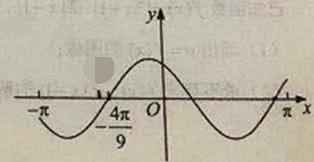
\includegraphics[width=.42\linewidth]{assets/asset-122-01.jpg}
\end{center}
\begin{choices}
  \item $\frac{10\pi}{9}$
  \item $\frac{7\pi}{6}$
  \item $\frac{4\pi}{3}$
  \item $\frac{3\pi}{2}$
\end{choices}
\begin{solution}
\textbf{答案：}C

\textbf{详解：}由图可得函数图象过点$\left(-\frac{4\pi}{9},0\right)$，代入得$\cos\left(-\frac{4\pi}{9}\omega+\frac{\pi}{6}\right)=0$。又该点是函数图象与$x$轴负半轴的第一个交点，所以$-\frac{4\pi}{9}\omega+\frac{\pi}{6}=-\frac{\pi}{2}$，解得$\omega=\frac{3}{2}$，因此最小正周期$T=\frac{2\pi}{\omega}=\frac{4\pi}{3}$。
\end{solution}
\end{question}

\begin{question}[points=5]
\textbf{来源：}2020 年 全国I卷-理科，第 9 题\quad \textbf{专题：}三角函数\par
已知$\alpha\in(0,\pi)$，且$3\cos2\alpha-8\cos\alpha=5$，则$\sin\alpha=$
\begin{choices}
  \item $\frac{\sqrt{5}}{3}$
  \item $\frac{2}{3}$
  \item $\frac{1}{3}$
  \item $\frac{\sqrt{5}}{9}$
\end{choices}
\begin{solution}
\textbf{答案：}A

\textbf{详解：}由$3\cos2\alpha-8\cos\alpha=5$得$3(2\cos^2\alpha-1)-8\cos\alpha=5$，即$6\cos^2\alpha-8\cos\alpha-8=0$，化简得$3\cos^2\alpha-4\cos\alpha-4=0$，解得$\cos\alpha=-\frac{2}{3}$或$\cos\alpha=2$（舍去）。因为$\alpha\in(0,\pi)$，所以$\sin\alpha=\sqrt{1-\cos^2\alpha}=\frac{\sqrt{5}}{3}$。
\end{solution}
\end{question}

\begin{question}[points=5]
\textbf{来源：}2020 年 全国I卷-理科，第 14 题\quad \textbf{专题：}向量\par
设$a,b$为单位向量，且$|a+b|=1$，则$|a-b|=$。
\fillin[{$\sqrt{3}$}]
\begin{solution}
\textbf{答案：}$\sqrt{3}$

\textbf{详解：}因为$a,b$为单位向量，所以$|a|=|b|=1$。由$|a+b|^2=a^2+2a\cdot b+b^2=2+2a\cdot b=1$，得$2a\cdot b=-1$。故$|a-b|^2=a^2-2a\cdot b+b^2=2-(-1)=3$，所以$|a-b|=\sqrt{3}$。
\end{solution}
\end{question}

\begin{question}[points=5]
\textbf{来源：}2020 年 全国I卷-理科，第 16 题\quad \textbf{专题：}三角函数\par
如图，在三棱锥$P-ABC$的平面展开图中，$AC=1$，$AB=AD=\sqrt{3}$，$AB\perp AC$，$AB\perp AD$，$\angle CAE=30^\circ$，则$\cos\angle FCB=$。

\begin{center}
  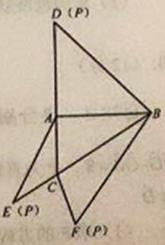
\includegraphics[width=.42\linewidth]{assets/asset-125-01.jpg}
\end{center}
\fillin[{$-\frac{1}{4}$}]
\begin{solution}
\textbf{答案：}$-\frac{1}{4}$

\textbf{详解：}由$AB\perp AC$，$AB=\sqrt{3}$，$AC=1$，由勾股定理得$BC=2$。同理$BD=\sqrt{AB^2+AD^2}=\sqrt{6}$，所以$BF=BD=\sqrt{6}$。在$\triangle ACE$中，$AC=1$，$AE=AD=\sqrt{3}$，$\angle CAE=30^\circ$，由余弦定理得$CE^2=AC^2+AE^2-2AC\cdot AE\cos30^\circ=1+3-2\times1\times\sqrt{3}\times\frac{\sqrt{3}}{2}=1$，所以$CF=CE=1$。在$\triangle BCF$中，$BC=2$，$BF=\sqrt{6}$，$CF=1$，由余弦定理得$\cos\angle FCB=\frac{CF^2+BC^2-BF^2}{2CF\cdot BC}=\frac{1+4-6}{2\times1\times2}=-\frac{1}{4}$。
\end{solution}
\end{question}

\begin{question}[points=12]
\textbf{来源：}2020 年 全国I卷-理科，第 20 题\quad \textbf{专题：}向量\par
已知$A,B$分别为椭圆$E:\frac{x^2}{a^2}+y^2=1(a>1)$的左、右顶点，$G$为$E$的上顶点，$\overrightarrow{AG}\cdot\overrightarrow{GB}=8$。$P$为直线$x=6$上的动点，$PA$与$E$的另一交点为$C$，$PB$与$E$的另一交点为$D$。

(1)求$E$的方程；

(2)证明：直线$CD$过定点。
\begin{solution}
\textbf{答案：}(1)$\frac{x^2}{9}+y^2=1$；(2)直线$CD$过定点$\left(\frac{3}{2},0\right)$

\textbf{详解：}(1)由椭圆方程得$A(-a,0),B(a,0),G(0,1)$，则$\overrightarrow{AG}=(a,1),\overrightarrow{GB}=(a,-1)$，$\overrightarrow{AG}\cdot\overrightarrow{GB}=a^2-1=8$，解得$a^2=9$，故椭圆方程为$\frac{x^2}{9}+y^2=1$。
(2)设$P(6,y_0)$，则直线$AP$方程为$y=\frac{y_0}{9}(x+3)$，与椭圆联立得$(y_0^2+9)x^2+6y_0^2x+9y_0^2-81=0$，由韦达定理$x_A\cdot x_C=\frac{9y_0^2-81}{y_0^2+9}$，而$x_A=-3$，得$x_C=\frac{-3y_0^2+27}{y_0^2+9}$，代入得$y_C=\frac{6y_0}{y_0^2+9}$，故$C\left(\frac{-3y_0^2+27}{y_0^2+9},\frac{6y_0}{y_0^2+9}\right)$。同理直线$PB$方程$y=\frac{y_0}{3}(x-3)$，与椭圆联立得$D\left(\frac{3y_0^2-3}{y_0^2+1},\frac{-2y_0}{y_0^2+1}\right)$。当$y_0\neq0$时，直线$CD$斜率$k=\frac{\frac{6y_0}{y_0^2+9}-\frac{-2y_0}{y_0^2+1}}{\frac{-3y_0^2+27}{y_0^2+9}-\frac{3y_0^2-3}{y_0^2+1}}=\frac{4y_0}{3(3-y_0^2)}$，直线$CD$方程为$y-\frac{-2y_0}{y_0^2+1}=\frac{4y_0}{3(3-y_0^2)}\left(x-\frac{3y_0^2-3}{y_0^2+1}\right)$，化简得$y=\frac{4y_0}{3(3-y_0^2)}\left(x-\frac{3}{2}\right)$，故过定点$\left(\frac{3}{2},0\right)$。当$y_0=0$时，$C(3,0),D(3,0)$，直线$CD$为$x=3$，也过$\left(\frac{3}{2},0\right)$。综上，直线$CD$过定点$\left(\frac{3}{2},0\right)$。
\end{solution}
\end{question}

\begin{question}[points=5]
\textbf{来源：}2020 年 全国I卷-文科，第 7 题\quad \textbf{专题：}三角函数\par
设函数 $f(x) = \cos\left(\omega x + \frac{\pi}{6}\right)$ 在 $[-\pi,\pi]$ 的图像大致如下图，则 $f(x)$ 的最小正周期为

\begin{center}
  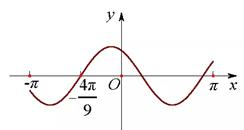
\includegraphics[width=.42\linewidth]{assets/asset-127-01.jpg}
\end{center}
\begin{choices}
  \item $\frac{10\pi}{9}$
  \item $\frac{7\pi}{6}$
  \item $\frac{4\pi}{3}$
  \item $\frac{3\pi}{2}$
\end{choices}
\begin{solution}
\textbf{答案：}$\frac{4\pi}{3}$

\textbf{分析：}由图可得函数图象过点 $\left(-\frac{4\pi}{9},0\right)$, 代入得到 $\cos\left(-\frac{4\pi}{9}\omega + \frac{\pi}{6}\right) = 0$, 结合点 $\left(-\frac{4\pi}{9},0\right)$ 是函数图象与 $x$ 轴负半轴的第一个交点得到 $-\frac{4\pi}{9}\omega + \frac{\pi}{6} = -\frac{\pi}{2}$, 解得 $\omega = \frac{3}{2}$, 再利用周期公式即可得解.

\textbf{详解：}由图可得函数图象过点 $\left(-\frac{4\pi}{9},0\right)$, 代入得 $\cos\left(-\frac{4\pi}{9}\omega + \frac{\pi}{6}\right) = 0$. 点 $\left(-\frac{4\pi}{9},0\right)$ 是函数图象与 $x$ 轴负半轴的第一个交点，所以 $-\frac{4\pi}{9}\omega + \frac{\pi}{6} = -\frac{\pi}{2}$, 解得 $\omega = \frac{3}{2}$. 所以函数 $f(x)$ 的最小正周期为 $T = \frac{2\pi}{\omega} = \frac{2\pi}{3/2} = \frac{4\pi}{3}$.
\end{solution}
\end{question}

\begin{question}[points=5]
\textbf{来源：}2020 年 全国I卷-文科，第 14 题\quad \textbf{专题：}向量\par
设向量 $\vec{a} = (1, -1)$, $\vec{b} = (m+1, 2m-4)$, 若 $\vec{a} \perp \vec{b}$, 则 $m =$
\fillin[{$5$}]
\begin{solution}
\textbf{答案：}$5$

\textbf{分析：}根据向量垂直的坐标表示求得结果.

\textbf{详解：}由 $\vec{a} \perp \vec{b}$ 可得 $\vec{a} \cdot \vec{b} = 0$, 即 $1\cdot(m+1) + (-1)\cdot(2m-4) = 0$, 解得 $m=5$.
\end{solution}
\end{question}

\begin{question}[points=12]
\textbf{来源：}2020 年 全国I卷-文科，第 18 题\quad \textbf{专题：}三角函数\par
$\triangle ABC$ 的内角 $A, B, C$ 的对边分别为 $a, b, c$. 已知 $B=150^\circ$.



(1) 若 $a=\sqrt{3}c$, $b=2\sqrt{7}$, 求 $\triangle ABC$ 的面积;



(2) 若 $\sin A + \sqrt{3}\sin C = \frac{\sqrt{2}}{2}$, 求 $C$.
\begin{solution}
\textbf{答案：}(1) $\sqrt{3}$; (2) $15^\circ$.

\textbf{分析：}(1) 已知角 $B$ 和 $b$ 边，结合 $a,c$ 关系，由余弦定理建立 $c$ 的方程，求解得出 $a,c$, 利用面积公式，即可得出结论； (2) 将 $A=30^\circ - C$ 代入已知等式，由两角差的正弦和辅助角公式，化简得出有关 $C$ 角的三角函数值，结合 $C$ 的范围，即可求解.

\textbf{详解：}(1) 由余弦定理可得 $b^2 = 28 = a^2 + c^2 - 2ac\cos150^\circ = 7c^2$, 所以 $c=2$, $a=2\sqrt{3}$, $\triangle ABC$ 的面积 $S = \frac{1}{2}ac\sin B = \sqrt{3}$.

(2) 因为 $A+C=30^\circ$, 所以 $\sin A + \sqrt{3}\sin C = \sin(30^\circ - C) + \sqrt{3}\sin C = \frac{1}{2}\cos C + \frac{\sqrt{3}}{2}\sin C = \sin(C+30^\circ) = \frac{\sqrt{2}}{2}$. 因为 $0^\circ < C < 30^\circ$, 所以 $30^\circ < C+30^\circ < 60^\circ$, 所以 $C+30^\circ = 45^\circ$, 即 $C=15^\circ$.
\end{solution}
\end{question}

\begin{question}[points=12]
\textbf{来源：}2020 年 全国I卷-文科，第 21 题\quad \textbf{专题：}向量\par
已知 $A, B$ 分别为椭圆 $E: \frac{x^2}{a^2} + y^2 = 1$ ($a>1$) 的左、右顶点，$G$ 为 $E$ 的上顶点，$\overrightarrow{AG} \cdot \overrightarrow{GB} = 8$, $P$ 为直线 $x=6$ 上的动点，$PA$ 与 $E$ 的另一交点为 $C$, $PB$ 与 $E$ 的另一交点为 $D$.



(1) 求 $E$ 的方程;



(2) 证明：直线 $CD$ 过定点.
\begin{solution}
\textbf{答案：}(1) $\frac{x^2}{9} + y^2 = 1$; (2) 证明见解析, 定点为 $\left(\frac{3}{2}, 0\right)$.

\textbf{分析：}(1) 由已知可得 $A(-a,0)$, $B(a,0)$, $G(0,1)$, 即可求得 $\overrightarrow{AG}\cdot\overrightarrow{GB}=a^2-1$, 结合已知即可求得 $a^2=9$; (2) 设 $P(6,y_0)$, 联立直线 $AP$ 与椭圆方程求得点 $C$ 坐标，同理求得点 $D$ 坐标，表示出直线 $CD$ 的方程，整理可得直线 $CD$ 过定点 $\left(\frac{3}{2},0\right)$.

\textbf{详解：}(1) 由椭圆方程得 $A(-a,0)$, $B(a,0)$, $G(0,1)$, 则 $\overrightarrow{AG}=(a,1)$, $\overrightarrow{GB}=(a,-1)$, 所以 $\overrightarrow{AG}\cdot\overrightarrow{GB}=a^2-1=8$, 解得 $a^2=9$, 故椭圆方程为 $\frac{x^2}{9}+y^2=1$.

(2) 设 $P(6,y_0)$, 则直线 $AP$ 的方程为 $y=\frac{y_0}{9}(x+3)$. 联立 $\begin{cases} \frac{x^2}{9}+y^2=1 \\ y=\frac{y_0}{9}(x+3) \end{cases}$, 消 $y$ 得 $(y_0^2+9)x^2+6y_0^2x+9y_0^2-81=0$, 由韦达定理知 $x_A x_C = \frac{9y_0^2-81}{y_0^2+9}$, 又 $x_A=-3$, 所以 $x_C = \frac{-3y_0^2+27}{y_0^2+9}$, 代入直线 $AP$ 得 $y_C = \frac{6y_0}{y_0^2+9}$, 即 $C\left(\frac{-3y_0^2+27}{y_0^2+9}, \frac{6y_0}{y_0^2+9}\right)$. 同理，直线 $PB$ 的方程为 $y=\frac{y_0}{3}(x-3)$, 联立解得 $D\left(\frac{3y_0^2-3}{y_0^2+1}, \frac{-2y_0}{y_0^2+1}\right)$. 则直线 $CD$ 的斜率 $k_{CD} = \frac{\frac{6y_0}{y_0^2+9} - \frac{-2y_0}{y_0^2+1}}{\frac{-3y_0^2+27}{y_0^2+9} - \frac{3y_0^2-3}{y_0^2+1}} = \frac{8y_0(y_0^2+3)}{6(9-y_0^4)} = \frac{4y_0}{3(3-y_0^2)}$, 所以直线 $CD$ 的方程为 $y - \frac{-2y_0}{y_0^2+1} = \frac{4y_0}{3(3-y_0^2)}\left(x - \frac{3y_0^2-3}{y_0^2+1}\right)$, 化简得 $y = \frac{4y_0}{3(3-y_0^2)}\left(x - \frac{3}{2}\right)$, 所以直线 $CD$ 过定点 $\left(\frac{3}{2},0\right)$.
\end{solution}
\end{question}

\section*{2021 年}

\begin{question}[points=4]
\textbf{来源：}2021 年 北京卷，第 7 题\quad \textbf{专题：}三角函数\par
函数 $f(x)=\cos x-\cos 2x$, 试判断函数的奇偶性及最大值（ ）
\begin{choices}
  \item 奇函数, 最大值为 $2$
  \item 偶函数, 最大值为 $2$
  \item 奇函数, 最大值为 $\frac{9}{8}$
  \item 偶函数, 最大值为 $\frac{9}{8}$
\end{choices}
\begin{solution}
\textbf{答案：}D

\textbf{分析：}由函数奇偶性的定义结合三角函数的性质可判断奇偶性; 利用二倍角公式结合二次函数的性质可判断最大值.

\textbf{详解：}由题意, $f(-x)=\cos(-x)-\cos(-2x)=\cos x-\cos 2x=f(x)$, 所以该函数为偶函数, 又 $f(x)=\cos x-\cos 2x=-2\cos^2 x+\cos x+1=-2\left(\cos x-\frac{1}{4}\right)^2+\frac{9}{8}$, 所以当 $\cos x=\frac{1}{4}$ 时, $f(x)$ 取最大值 $\frac{9}{8}$.
\end{solution}
\end{question}

\begin{question}[points=5]
\textbf{来源：}2021 年 北京卷，第 13 题\quad \textbf{专题：}向量\par
$\vec{a}=(2,1)$, $\vec{b}=(2,-1)$, $\vec{c}=(0,1)$, 则 $(\vec{a}+\vec{b})\cdot\vec{c}=$ ； $\vec{a}\cdot\vec{b}=$ .
\fillin[{$0$；$3$}]
\begin{solution}
\textbf{答案：}$0$；$3$

\textbf{分析：}根据坐标求出 $\vec{a}+\vec{b}$, 再根据数量积的坐标运算直接计算即可.

\textbf{详解：}$\vec{a}+\vec{b}=(4,0)$, $\vec{a}\cdot\vec{c}=4\times0+0\times1=0$, $\vec{a}\cdot\vec{b}=2\times2+1\times(-1)=3$.
\end{solution}
\end{question}

\begin{question}[points=5]
\textbf{来源：}2021 年 北京卷，第 14 题\quad \textbf{专题：}三角函数\par
若点 $P(\cos\theta,\sin\theta)$ 与点 $Q(\cos(\theta+\frac{\pi}{6}),\sin(\theta+\frac{\pi}{6}))$ 关于 $y$ 轴对称, 写出一个符合题意的 $\theta=$ .
\fillin[{$\frac{5\pi}{12}$（满足 $\theta=\frac{5\pi}{12}+k\pi, k\in\mathbb{Z}$ 即可）}]
\begin{solution}
\textbf{答案：}$\frac{5\pi}{12}$（满足 $\theta=\frac{5\pi}{12}+k\pi, k\in\mathbb{Z}$ 即可）

\textbf{分析：}根据 $P,Q$ 在单位圆上, 可得 $\theta,\theta+\frac{\pi}{6}$ 关于 $y$ 轴对称, 得出 $\theta+\frac{\pi}{6}+\theta=\pi+2k\pi, k\in\mathbb{Z}$ 求解.

\textbf{详解：}$\because P(\cos\theta,\sin\theta)$ 与 $Q(\cos(\theta+\frac{\pi}{6}),\sin(\theta+\frac{\pi}{6}))$ 关于 $y$ 轴对称, 即 $\theta,\theta+\frac{\pi}{6}$ 关于 $y$ 轴对称, $\theta+\frac{\pi}{6}+\theta=\pi+2k\pi, k\in\mathbb{Z}$, 则 $\theta=k\pi+\frac{5\pi}{12}, k\in\mathbb{Z}$, 当 $k=0$ 时, 可取 $\theta$ 的一个值为 $\frac{5\pi}{12}$.
\end{solution}
\end{question}

\begin{question}[points=13]
\textbf{来源：}2021 年 北京卷，第 16 题\quad \textbf{专题：}三角形、三角函数\par
已知在 $\triangle ABC$ 中, $c=2b\cos B$, $C=\frac{2\pi}{3}$.

(1) 求 $B$ 的大小;

(2) 在下列三个条件中选择一个作为已知, 使 $\triangle ABC$ 存在且唯一确定, 并求出 $BC$ 边上的中线的长度.

① $c=\sqrt{2}b$; ② 周长为 $4+2\sqrt{3}$; ③ 面积为 $S_{\triangle ABC}=\frac{3\sqrt{3}}{4}$.
\begin{solution}
\textbf{答案：}(1) $B=\frac{\pi}{6}$; (2) 若选择②, 中线长为 $\sqrt{7}$; 若选择③, 中线长为 $\frac{\sqrt{21}}{2}$.

\textbf{分析：}(1) 由正弦定理化边为角即可求解; (2) 分别分析每个条件, 选择使三角形存在且唯一确定的, 利用余弦定理求解中线长.

\textbf{详解：}(1) 由 $c=2b\cos B$, 正弦定理得 $\sin C=2\sin B\cos B$, 即 $\sin 2B=\sin C=\sin\frac{2\pi}{3}=\frac{\sqrt{3}}{2}$, 又 $C=\frac{2\pi}{3}$, $B\in(0,\frac{\pi}{3})$, $2B\in(0,\frac{2\pi}{3})$, 所以 $2B=\frac{\pi}{3}$, 解得 $B=\frac{\pi}{6}$.
(2) 若选择①, 由正弦定理 $\frac{c}{b}=\frac{\sin C}{\sin B}=\frac{\sqrt{3}/2}{1/2}=\sqrt{3}$, 与 $c=\sqrt{2}b$ 矛盾, 故不存在.
若选择②, 由(1)得 $A=\pi-\frac{2\pi}{3}-\frac{\pi}{6}=\frac{\pi}{6}$, 则 $a=b$. 设外接圆半径为 $R$, 则 $a=b=2R\sin\frac{\pi}{6}=R$, $c=2R\sin\frac{2\pi}{3}=\sqrt{3}R$, 周长 $a+b+c=2R+\sqrt{3}R=4+2\sqrt{3}$, 解得 $R=2$, 则 $a=2$, $c=2\sqrt{3}$. 由余弦定理, $BC$ 边上的中线长 $m=\sqrt{b^2+(\frac{a}{2})^2-2\cdot b\cdot\frac{a}{2}\cdot\cos C}=\sqrt{(2)^2+1^2-2\times2\times1\times\cos\frac{2\pi}{3}}=\sqrt{4+1+2}=\sqrt{7}$.
若选择③, 由(1)得 $A=\frac{\pi}{6}$, 则 $a=b$. 面积 $S=\frac{1}{2}ab\sin C=\frac{1}{2}a^2\times\frac{\sqrt{3}}{2}=\frac{3\sqrt{3}}{4}$, 解得 $a=3$, 则 $b=3$, $c=2b\cos B=2\times3\times\frac{\sqrt{3}}{2}=3\sqrt{3}$. 由余弦定理, $BC$ 边上的中线长 $m=\sqrt{b^2+(\frac{a}{2})^2-2\cdot b\cdot\frac{a}{2}\cdot\cos C}=\sqrt{9+\frac{9}{4}-2\times3\times\frac{3}{2}\times\cos\frac{2\pi}{3}}=\sqrt{9+\frac{9}{4}+\frac{9}{2}}=\sqrt{\frac{36+9+18}{4}}=\sqrt{\frac{63}{4}}=\frac{3\sqrt{7}}{2}$.
\end{solution}
\end{question}

\begin{question}[points=5]
\textbf{来源：}2021 年 全国甲卷-理科，第 5 题\quad \textbf{专题：}三角形\par
已知 $F_1, F_2$ 是双曲线 $C$ 的两个焦点，$P$ 为 $C$ 上一点，且 $\angle F_1PF_2 = 60^\circ$, $|PF_1| = 3|PF_2|$，则 $C$ 的离心率为（ ）
\begin{choices}
  \item $\frac{\sqrt{7}}{2}$
  \item $\frac{\sqrt{13}}{2}$
  \item $\sqrt{7}$
  \item $\sqrt{13}$
\end{choices}
\begin{solution}
\textbf{答案：}A

\textbf{分析：}根据双曲线的定义及条件，表示出 $PF_1, PF_2$，结合余弦定理可得答案．

\textbf{详解：}由双曲线的定义可得 $|PF_1|-|PF_2| = 2|PF_2| = 2a$, 所以 $|PF_2| = a$, $|PF_1| = 3a$；在 $\triangle F_1PF_2$ 中，由余弦定理得 $4c^2 = 9a^2 + a^2 - 2\cdot 3a\cdot a\cos60^\circ$, 解得 $4c^2 = 7a^2$, 所以 $e^2 = \frac{c^2}{a^2} = \frac{7}{4}$, 即 $e = \frac{\sqrt{7}}{2}$．
\end{solution}
\end{question}

\begin{question}[points=5]
\textbf{来源：}2021 年 全国甲卷-理科，第 8 题\quad \textbf{专题：}三角形、三角函数\par
2020年12月8日，中国和尼泊尔联合公布珠穆朗玛峰最新高程为8848.86（单位：m），三角高程测量法是珠峰高程测量方法之一．如图是三角高程测量法的一个示意图，现有 $A, B, C$ 三点，且 $A, B, C$ 在同一水平面上的投影 $A', B', C'$ 满足 $\angle A'C'B' = 45^\circ$, $\angle A'B'C' = 60^\circ$．由 $C$ 点测得 $B$ 点的仰角为 $15^\circ$, $BB'$ 与 $CC'$ 的差为100；由 $B$ 点测得 $A$ 点的仰角为 $45^\circ$，则 $A, C$ 两点到水平面 $A'B'C'$ 的高度差 $AA' - CC'$ 约为（$\sqrt{3} \approx 1.732$）（ ）

\begin{center}
  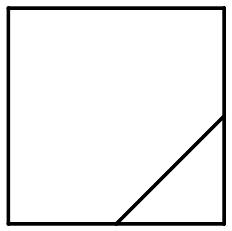
\includegraphics[width=.42\linewidth]{assets/asset-136-01.jpg}
\end{center}
\begin{choices}
  \item $346$
  \item $373$
  \item $446$
  \item $473$
\end{choices}
\begin{solution}
\textbf{答案：}B

\textbf{分析：}通过做辅助线，将已知所求量转化到一个三角形中，借助正弦定理，求得 $A'B'$，进而得到答案．

\textbf{详解：}过 $C$ 作 $CH \perp BB'$，过 $B$ 作 $BD \perp AA'$，则 $AA' - CC' = AA' - (BB' - BH) = AA' - BB' + 100 = AD + 100$．由题易知 $\triangle ADB$ 为等腰直角三角形，所以 $AD = DB$，故 $AA' - CC' = DB + 100 = A'B' + 100$．因为 $\angle BCH = 15^\circ$，所以 $CH = C'B' = \frac{100}{\tan 15^\circ}$．在 $\triangle A'B'C'$ 中，由正弦定理得 $\frac{A'B'}{\sin 45^\circ} = \frac{C'B'}{\sin 75^\circ} = \frac{100}{\tan 15^\circ \cos 15^\circ \sin 15^\circ}$，而 $\sin 15^\circ = \frac{\sqrt{6}-\sqrt{2}}{4}$，得 $A'B' = 100(\sqrt{3}+1) \approx 273$，所以 $AA' - CC' \approx 373$．
\end{solution}
\end{question}

\begin{question}[points=5]
\textbf{来源：}2021 年 全国甲卷-理科，第 9 题\quad \textbf{专题：}三角函数\par
若 $\alpha \in \left(0, \frac{\pi}{2}\right)$, $\tan 2\alpha = \frac{\cos \alpha}{2 - \sin \alpha}$, 则 $\tan \alpha = $ ( )
\begin{choices}
  \item $\frac{\sqrt{15}}{15}$
  \item $\frac{\sqrt{5}}{5}$
  \item $\frac{\sqrt{5}}{3}$
  \item $\frac{\sqrt{15}}{3}$
\end{choices}
\begin{solution}
\textbf{答案：}A

\textbf{分析：}由二倍角公式可得 $\tan 2\alpha = \frac{\sin 2\alpha}{\cos 2\alpha} = \frac{2\sin \alpha \cos \alpha}{1-2\sin^2 \alpha}$，再结合已知可求得 $\sin \alpha = \frac{1}{4}$，利用同角三角函数的基本关系即可求解．

\textbf{详解：}由条件得 $\frac{2\sin \alpha \cos \alpha}{1-2\sin^2 \alpha} = \frac{\cos \alpha}{2-\sin \alpha}$，因为 $\cos \alpha \neq 0$，所以 $\frac{2\sin \alpha}{1-2\sin^2 \alpha} = \frac{1}{2-\sin \alpha}$，解得 $\sin \alpha = \frac{1}{4}$，则 $\cos \alpha = \frac{\sqrt{15}}{4}$，故 $\tan \alpha = \frac{\sqrt{15}}{15}$．
\end{solution}
\end{question}

\begin{question}[points=5]
\textbf{来源：}2021 年 全国甲卷-理科，第 14 题\quad \textbf{专题：}向量\par
已知向量 $\vec{a} = (3,1)$, $\vec{b} = (1,0)$, $\vec{c} = \vec{a} + k\vec{b}$．若 $\vec{a} \perp \vec{c}$，则 $k = $ ．
\fillin[{$-\frac{10}{3}$}]
\begin{solution}
\textbf{答案：}$-\frac{10}{3}$

\textbf{分析：}利用向量的坐标运算法则求得向量 $\vec{c}$ 的坐标，利用向量的数量积为零求得 $k$ 的值．

\textbf{详解：}$\vec{c} = (3+k, 1)$，由 $\vec{a} \perp \vec{c}$ 得 $3(3+k) + 1\times 1 = 0$，解得 $k = -\frac{10}{3}$．
\end{solution}
\end{question}

\begin{question}[points=5]
\textbf{来源：}2021 年 全国甲卷-理科，第 16 题\quad \textbf{专题：}三角函数\par
已知函数 $f(x) = 2\cos(\omega x + \varphi)$ 的部分图像如图所示，则满足条件 $\left(f(x) - f\left(-\frac{7\pi}{4}\right)\right) \left(f(x) - f\left(\frac{4\pi}{3}\right)\right) > 0$ 的最小正整数 $x$ 为．

\begin{center}
  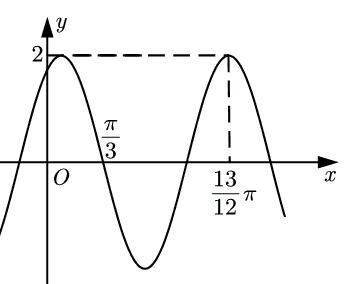
\includegraphics[width=.42\linewidth]{assets/asset-139-01.jpg}
\end{center}
\fillin[{$2$}]
\begin{solution}
\textbf{答案：}$2$

\textbf{分析：}先根据图象求出函数 $f(x)$ 的解析式，再求出 $f(-\frac{7\pi}{4}), f(\frac{4\pi}{3})$ 的值，然后求解三角不等式可得最小正整数或验证数值可得．

\textbf{详解：}由图可知 $\frac{3}{4}T = \frac{13\pi}{12} - \frac{\pi}{3} = \frac{3\pi}{4}$，所以 $T = \pi$，$\omega = 2$；由五点法得 $2\cdot\frac{\pi}{3} + \varphi = \frac{\pi}{2}$，所以 $\varphi = -\frac{\pi}{6}$，故 $f(x) = 2\cos\left(2x - \frac{\pi}{6}\right)$．计算得 $f\left(-\frac{7\pi}{4}\right) = 2\cos\left(-\frac{11\pi}{3}\right) = 2\cos\frac{\pi}{3} = 1$，$f\left(\frac{4\pi}{3}\right) = 2\cos\left(\frac{5\pi}{2}\right) = 0$，所以不等式化为 $(f(x)-1)f(x) > 0$，即 $f(x) > 1$ 或 $f(x) < 0$．通过验证最小正整数 $x=1$ 时，$f(1) = 2\cos\left(2 - \frac{\pi}{6}\right) < 1$；$x=2$ 时，$f(2) = 2\cos\left(4 - \frac{\pi}{6}\right) < 0$，故最小正整数 $x=2$．
\end{solution}
\end{question}

\begin{question}[points=10]
\textbf{来源：}2021 年 全国甲卷-理科，第 22 题\quad \textbf{专题：}向量\par
在直角坐标系 $xOy$ 中，以坐标原点为极点，$x$ 轴正半轴为极轴建立极坐标系，曲线 $C$ 的极坐标方程为 $\rho = 2\sqrt{2}\cos\theta$．（1）将 $C$ 的极坐标方程化为直角坐标方程；（2）设点 $A$ 的直角坐标为 $(1,0)$，$M$ 为 $C$ 上的动点，点 $P$ 满足 $\overrightarrow{AP} = \sqrt{2}\overrightarrow{AM}$，写出 $P$ 的轨迹 $C_1$ 的参数方程，并判断 $C$ 与 $C_1$ 是否有公共点．
\begin{solution}
\textbf{答案：}（1）$(x-\sqrt{2})^2+y^2=2$；（2）$P$ 的轨迹 $C_1$ 的参数方程为 $\begin{cases} x = 3-\sqrt{2}+\sqrt{2}\cos\theta \\ y = \sqrt{2}\sin\theta \end{cases}$（$\theta$ 为参数），$C$ 与 $C_1$ 没有公共点．

\textbf{分析：}（1）将曲线 $C$ 的极坐标方程化为 $\rho^2 = 2\sqrt{2}\rho\cos\theta$，将 $x=\rho\cos\theta, y=\rho\sin\theta$ 代入可得；（2）设 $P(x,y)$，设 $M(\sqrt{2}+\sqrt{2}\cos\theta, \sqrt{2}\sin\theta)$，根据向量关系即可求得 $P$ 的轨迹 $C_1$ 的参数方程，求出两圆圆心距，和半径之差比较可得．

\textbf{详解：}（1）由 $\rho=2\sqrt{2}\cos\theta$ 得 $\rho^2=2\sqrt{2}\rho\cos\theta$，即 $x^2+y^2=2\sqrt{2}x$，故 $(x-\sqrt{2})^2+y^2=2$．（2）设 $M(\sqrt{2}+\sqrt{2}\cos\theta, \sqrt{2}\sin\theta)$，$P(x,y)$，由 $\overrightarrow{AP}=\sqrt{2}\overrightarrow{AM}$ 得 $(x-1,y)=\sqrt{2}(\sqrt{2}+\sqrt{2}\cos\theta-1, \sqrt{2}\sin\theta)$，即 $\begin{cases} x = 3-\sqrt{2}+\sqrt{2}\cos\theta \\ y = \sqrt{2}\sin\theta \end{cases}$，为 $C_1$ 的参数方程．$C$ 的圆心 $C(\sqrt{2},0)$，半径 $r=\sqrt{2}$；$C_1$ 的圆心 $C_1(3-\sqrt{2},0)$，半径 $R=\sqrt{2}$，圆心距 $|CC_1| = 3-2\sqrt{2} \approx 0.172$，$R-r = 0$，故两圆内含，无公共点．
\end{solution}
\end{question}

\begin{question}[points=5]
\textbf{来源：}2021 年 全国甲卷-文科，第 8 题\quad \textbf{专题：}三角形\par
在 $\triangle ABC$ 中，已知 $B=120^{\circ}$, $AC=\sqrt{19}$, $AB=2$, 则 $BC=$ ( )
\begin{choices}
  \item 1
  \item $\sqrt{2}$
  \item $\sqrt{5}$
  \item 3
\end{choices}
\begin{solution}
\textbf{答案：}D

\textbf{分析：}利用余弦定理得到关于 $BC$ 长度的方程，解方程即可求得边长.

\textbf{详解：}设 $AB=c$, $AC=b$, $BC=a$, 结合余弦定理：$b^2 = a^2 + c^2 - 2ac \cos B$ 可得：$19 = a^2 + 4 - 2 \times a \times \cos 120^{\circ}$, 即 $a^2 + 2a -15 = 0$, 解得 $a=3$（$a=-5$ 舍去），故 $BC=3$.
\end{solution}
\end{question}

\begin{question}[points=5]
\textbf{来源：}2021 年 全国甲卷-文科，第 11 题\quad \textbf{专题：}三角函数\par
若 $\alpha \in \left(0, \frac{\pi}{2}\right)$, $\tan 2\alpha = \frac{\cos \alpha}{2 - \sin \alpha}$, 则 $\tan \alpha =$ ( )
\begin{choices}
  \item $\frac{\sqrt{15}}{15}$
  \item $\frac{\sqrt{5}}{5}$
  \item $\frac{\sqrt{5}}{3}$
  \item $\frac{\sqrt{15}}{3}$
\end{choices}
\begin{solution}
\textbf{答案：}A

\textbf{分析：}由二倍角公式可得 $\tan 2\alpha = \frac{\sin 2\alpha}{\cos 2\alpha} = \frac{2\sin\alpha\cos\alpha}{1-2\sin^2\alpha}$, 再结合已知可求得 $\sin\alpha = \frac{1}{4}$, 利用同角三角函数的基本关系即可求解.

\textbf{详解：}因为 $\tan 2\alpha = \frac{\cos\alpha}{2-\sin\alpha}$, 所以 $\tan 2\alpha = \frac{\sin 2\alpha}{\cos 2\alpha} = \frac{2\sin\alpha\cos\alpha}{1-2\sin^2\alpha} = \frac{\cos\alpha}{2-\sin\alpha}$. 因为 $\alpha \in \left(0, \frac{\pi}{2}\right)$, 所以 $\cos\alpha \neq 0$, 所以 $\frac{2\sin\alpha}{1-2\sin^2\alpha} = \frac{1}{2-\sin\alpha}$, 解得 $\sin\alpha = \frac{1}{4}$. 所以 $\cos\alpha = \sqrt{1-\sin^2\alpha} = \frac{\sqrt{15}}{4}$, 所以 $\tan\alpha = \frac{\sin\alpha}{\cos\alpha} = \frac{\sqrt{15}}{15}$.
\end{solution}
\end{question}

\begin{question}[points=5]
\textbf{来源：}2021 年 全国甲卷-文科，第 13 题\quad \textbf{专题：}向量\par
若向量 $\vec{a}, \vec{b}$ 满足 $|\vec{a}|=3$, $|\vec{a}-\vec{b}|=5$, $\vec{a}\cdot\vec{b}=1$, 则 $|\vec{b}|=$ .
\fillin[{$3\sqrt{2}$}]
\begin{solution}
\textbf{答案：}$3\sqrt{2}$

\textbf{分析：}根据题目条件，利用 $|\vec{a}-\vec{b}|$ 模的平方可以得出答案.

\textbf{详解：}因为 $|\vec{a}-\vec{b}|=5$, 所以 $|\vec{a}-\vec{b}|^2 = |\vec{a}|^2 + |\vec{b}|^2 - 2\vec{a}\cdot\vec{b} = 9 + |\vec{b}|^2 - 2 = 25$, 所以 $|\vec{b}|^2 = 18$, $|\vec{b}| = 3\sqrt{2}$.
\end{solution}
\end{question}

\begin{question}[points=5]
\textbf{来源：}2021 年 全国甲卷-文科，第 15 题\quad \textbf{专题：}三角函数\par
已知函数 $f(x) = 2\cos(\omega x + \varphi)$ 的部分图像如图所示，则 $f\left(\frac{\pi}{2}\right) =$ .

\begin{center}
  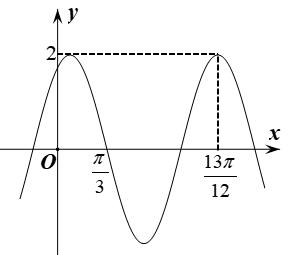
\includegraphics[width=.42\linewidth]{assets/asset-144-01.jpg}
\end{center}
\fillin[{$-\sqrt{3}$}]
\begin{solution}
\textbf{答案：}$-\sqrt{3}$

\textbf{分析：}首先确定函数的解析式，然后求解 $f\left(\frac{\pi}{2}\right)$ 的值即可.

\textbf{详解：}由题意可得：$\frac{3}{4}T = \frac{13\pi}{12} - \frac{\pi}{3} = \frac{3\pi}{4}$, 所以 $T = \pi$, $\omega = \frac{2\pi}{T} = 2$. 当 $x = \frac{13\pi}{12}$ 时，$\omega x + \varphi = 2 \times \frac{13\pi}{12} + \varphi = 2k\pi$, 所以 $\varphi = 2k\pi - \frac{13\pi}{6}$ ($k \in \mathbf{Z}$). 令 $k=1$ 可得：$\varphi = -\frac{\pi}{6}$. 据此有：$f(x) = 2\cos\left(2x - \frac{\pi}{6}\right)$, $f\left(\frac{\pi}{2}\right) = 2\cos\left(2\times\frac{\pi}{2} - \frac{\pi}{6}\right) = 2\cos\frac{5\pi}{6} = -\sqrt{3}$.
\end{solution}
\end{question}

\begin{question}[points=10]
\textbf{来源：}2021 年 全国甲卷-文科，第 22 题\quad \textbf{专题：}向量\par
[选修4-4：坐标系与参数方程]



在直角坐标系 $xOy$ 中，以坐标原点为极点，$x$ 轴正半轴为极轴建立极坐标系，曲线 $C$ 的极坐标方程为 $\rho = 2\sqrt{2}\cos\theta$.



（1）将 $C$ 的极坐标方程化为直角坐标方程；



（2）设点 $A$ 的直角坐标为 $(1,0)$, $M$ 为 $C$ 上的动点，点 $P$ 满足 $\overrightarrow{AP} = \sqrt{2}\overrightarrow{AM}$, 写出 $P$ 的轨迹 $C_1$ 的参数方程，并判断 $C$ 与 $C_1$ 是否有公共点．
\begin{solution}
\textbf{答案：}（1）$(x-\sqrt{2})^2 + y^2 = 2$；（2）$P$ 的轨迹 $C_1$ 的参数方程为 $\begin{cases} x = 3 - \sqrt{2} + \sqrt{2}\cos\theta \\ y = \sqrt{2}\sin\theta \end{cases}$ ($\theta$ 为参数)，$C$ 与 $C_1$ 没有公共点.

\textbf{分析：}（1）将曲线 $C$ 的极坐标方程化为 $\rho^2 = 2\sqrt{2}\rho\cos\theta$, 将 $x=\rho\cos\theta$, $y=\rho\sin\theta$ 代入可得；（2）设 $P(x,y)$, 设 $M(\sqrt{2}+\sqrt{2}\cos\theta, \sqrt{2}\sin\theta)$, 根据向量关系即可求得 $P$ 的轨迹 $C_1$ 的参数方程，求出两圆圆心距，和半径之差比较可得.

\textbf{详解：}（1）由曲线 $C$ 的极坐标方程 $\rho = 2\sqrt{2}\cos\theta$ 可得 $\rho^2 = 2\sqrt{2}\rho\cos\theta$, 将 $x=\rho\cos\theta$, $y=\rho\sin\theta$ 代入可得 $x^2+y^2 = 2\sqrt{2}x$, 即 $(x-\sqrt{2})^2 + y^2 = 2$.

（2）设 $P(x,y)$, 设 $M(\sqrt{2}+\sqrt{2}\cos\theta, \sqrt{2}\sin\theta)$. 因为 $\overrightarrow{AP} = \sqrt{2}\overrightarrow{AM}$, 所以 $(x-1, y) = \sqrt{2}(\sqrt{2}+\sqrt{2}\cos\theta - 1, \sqrt{2}\sin\theta) = (2+2\cos\theta - \sqrt{2}, 2\sin\theta)$. 则 $\begin{cases} x-1 = 2+2\cos\theta - \sqrt{2} \\ y = 2\sin\theta \end{cases}$, 即 $\begin{cases} x = 3 - \sqrt{2} + 2\cos\theta \\ y = 2\sin\theta \end{cases}$. 故 $P$ 的轨迹 $C_1$ 的参数方程为 $\begin{cases} x = 3 - \sqrt{2} + 2\cos\theta \\ y = 2\sin\theta \end{cases}$ ($\theta$ 为参数). 曲线 $C$ 的圆心为 $(\sqrt{2},0)$, 半径为 $\sqrt{2}$, 曲线 $C_1$ 的圆心为 $(3-\sqrt{2},0)$, 半径为 $2$, 则圆心距为 $3-2\sqrt{2}$, 因为 $3-2\sqrt{2} < 2 - \sqrt{2}$, 所以 两圆内含, 故曲线 $C$ 与 $C_1$ 没有公共点.
\end{solution}
\end{question}

\begin{question}[points=5]
\textbf{来源：}2021 年 全国乙卷-理科，第 3 题\quad \textbf{专题：}三角函数\par
已知命题$p:\exists x\in\mathbb{R}$，$\sin x<1$；命题$q:\forall x\in\mathbb{R}$，$e^{|x|}\geq 1$，则下列命题中为真命题的是（  ）
\begin{choices}
  \item $p\land q$
  \item $\lnot p\land q$
  \item $p\land \lnot q$
  \item $\lnot(p\lor q)$
\end{choices}
\begin{solution}
\textbf{答案：}$p\land q$

\textbf{详解：}根据正弦函数的值域$\sin x\in[-1,1]$，故$\exists x\in\mathbb{R}$，$\sin x<1$，$p$为真命题。函数$y=e^{|x|}$为偶函数，且$x\geq 0$时$y=e^{|x|}\geq 1$，故$\forall x\in\mathbb{R}$，$e^{|x|}\geq 1$恒成立，$q$也为真命题。所以$p\land q$为真。故选A。
\end{solution}
\end{question}

\begin{question}[points=5]
\textbf{来源：}2021 年 全国乙卷-理科，第 7 题\quad \textbf{专题：}三角函数\par
把函数$y=f(x)$图像上所有点的横坐标缩短到原来的$\frac12$倍，纵坐标不变，再把所得曲线向右平移$\frac{\pi}{3}$个单位长度，得到函数$y=\sin\left(x-\frac{\pi}{4}\right)$的图像，则$f(x)=$（  ）
\begin{choices}
  \item $\sin\left(\frac{x}{2}-\frac{7\pi}{12}\right)$
  \item $\sin\left(\frac{x}{2}+\frac{\pi}{12}\right)$
  \item $\sin\left(2x-\frac{7\pi}{12}\right)$
  \item $\sin\left(2x+\frac{\pi}{12}\right)$
\end{choices}
\begin{solution}
\textbf{答案：}$\sin\left(\frac{x}{2}+\frac{\pi}{12}\right)$

\textbf{详解：}逆向：$y=\sin\left(x-\frac{\pi}{4}\right) \xrightarrow{\text{左移}\frac{\pi}{3}} y=\sin\left(x+\frac{\pi}{12}\right) \xrightarrow{\text{横坐标变为原来的2倍}} y=\sin\left(\frac{x}{2}+\frac{\pi}{12}\right)$。故选B。
\end{solution}
\end{question}

\begin{question}[points=5]
\textbf{来源：}2021 年 全国乙卷-理科，第 14 题\quad \textbf{专题：}向量\par
已知向量$\vec{a}=(1,3)$，$\vec{b}=(3,4)$，若$(\vec{a}-\lambda\vec{b})\perp\vec{b}$，则$\lambda=$。
\fillin[{$\frac{3}{5}$}]
\begin{solution}
\textbf{答案：}$\frac{3}{5}$

\textbf{详解：}由题意得$(\vec{a}-\lambda\vec{b})\cdot\vec{b}=0$，即$15-25\lambda=0$，解得$\lambda=\frac{3}{5}$。
\end{solution}
\end{question}

\begin{question}[points=5]
\textbf{来源：}2021 年 全国乙卷-理科，第 15 题\quad \textbf{专题：}三角形\par
记$\triangle ABC$的内角$A$，$B$，$C$的对边分别为$a$，$b$，$c$，面积为$\sqrt{3}$，$B=60^\circ$，$a^2+c^2=3ac$，则$b=$。
\fillin[{$2\sqrt{2}$}]
\begin{solution}
\textbf{答案：}$2\sqrt{2}$

\textbf{详解：}$S_{\triangle ABC}=\frac12ac\sin B=\frac{\sqrt{3}}{4}ac=\sqrt{3}$，所以$ac=4$，由余弦定理，$b^2=a^2+c^2-2ac\cos B=3ac-ac=2ac=8$，所以$b=2\sqrt{2}$。
\end{solution}
\end{question}

\begin{question}[points=5]
\textbf{来源：}2021 年 全国乙卷-文科，第 3 题\quad \textbf{专题：}三角函数\par
已知命题 $p: \exists x \in \mathbb{R}, \sin x < 1$ ；命题 $q: \forall x \in \mathbb{R}, e^{|x|} \ge 1$ ，则下列命题中为真命题的是（ ）
\begin{choices}
  \item $p \land q$
  \item $\neg p \land q$
  \item $p \land \neg q$
  \item $\neg(p \lor q)$
\end{choices}
\begin{solution}
\textbf{答案：}A

\textbf{分析：}根据正弦函数的值域 $\sin x \in [-1,1]$ ， $\sin x < 1$ ，故 $\exists x \in \mathbb{R}$ ， $p$ 为真命题，而函数 $y = e^{|x|}$ 为偶函数，且 $x \ge 0$ 时，$y = e^x \ge 1$ ，故 $\forall x \in \mathbb{R}$ ， $y = e^{|x|} \ge 1$ 恒成立.则 $q$ 也为真命题，所以 $p \land q$ 为真，选 A.
\end{solution}
\end{question}

\begin{question}[points=5]
\textbf{来源：}2021 年 全国乙卷-文科，第 4 题\quad \textbf{专题：}三角函数\par
函数 $f(x) = \sin\frac{x}{3} + \cos\frac{x}{3}$ 的最小正周期和最大值分别是（ ）
\begin{choices}
  \item $3\pi$ 和 $\sqrt{2}$
  \item $3\pi$ 和 $2$
  \item $6\pi$ 和 $\sqrt{2}$
  \item $6\pi$ 和 $2$
\end{choices}
\begin{solution}
\textbf{答案：}C

\textbf{分析：}$f(x) = \sqrt{2}\sin\left(\frac{x}{3} + \frac{\pi}{4}\right)$ ，$f(x)_{\max} = \sqrt{2}$ ， $T = \frac{2\pi}{\frac{1}{3}} = 6\pi$ .
\end{solution}
\end{question}

\begin{question}[points=5]
\textbf{来源：}2021 年 全国乙卷-文科，第 6 题\quad \textbf{专题：}三角函数\par
$\cos^2\frac{\pi}{12} - \cos^2\frac{5\pi}{12} =$ （ ）
\begin{choices}
  \item $\frac{1}{2}$
  \item $\frac{\sqrt{3}}{3}$
  \item $\frac{\sqrt{2}}{2}$
  \item $\frac{\sqrt{3}}{2}$
\end{choices}
\begin{solution}
\textbf{答案：}D

\textbf{分析：}$\cos^2\frac{\pi}{12} - \cos^2\frac{5\pi}{12} = \cos^2\frac{\pi}{12} - \cos^2\left(\frac{\pi}{2} - \frac{\pi}{12}\right) = \cos^2\frac{\pi}{12} - \sin^2\frac{\pi}{12} = \cos\frac{\pi}{6} = \frac{\sqrt{3}}{2}$ .
\end{solution}
\end{question}

\begin{question}[points=5]
\textbf{来源：}2021 年 全国乙卷-文科，第 8 题\quad \textbf{专题：}三角函数\par
下列函数中最小值为4的是（ ）
\begin{choices}
  \item $y = x^2 + 2x + 4$
  \item $y = |\sin x| + \frac{4}{|\sin x|}$
  \item $y = 2^x + 2^{2-x}$
  \item $y = \ln x + \frac{4}{\ln x}$
\end{choices}
\begin{solution}
\textbf{答案：}C

\textbf{分析：}对于 A，$y = x^2 + 2x + 4 = (x+1)^2 + 3 \ge 3$ .不符合，
对于 B，$y = |\sin x| + \frac{4}{|\sin x|}$ ，令 $t = |\sin x| \in [0,1]$ ，$y = t + \frac{4}{t}$ ，根据对勾函数 $y_{\min} = 1 + 4 = 5$ 不符合，
对于 C，$y = 2^x + 2^{2-x} = 2^x + \frac{4}{2^x}$ ，令 $t = 2^x > 0$ ，$y = t + \frac{4}{t} \ge 2\sqrt{t \cdot \frac{4}{t}} = 4$ ，当且仅当 $t=2$ 时取等，符合，
对于 D，$y = \ln x + \frac{4}{\ln x}$ ，令 $t = \ln x \in \mathbb{R}$ ，$y = t + \frac{4}{t}$ ，根据对勾函数 $y \in (-\infty, -4] \cup [4, +\infty)$ ，不符合.
\end{solution}
\end{question}

\begin{question}[points=5]
\textbf{来源：}2021 年 全国乙卷-文科，第 13 题\quad \textbf{专题：}向量\par
已知向量 $\vec{a} = (2,5)$ ， $\vec{b} = (\lambda, 4)$ ，若 $\vec{a} // \vec{b}$ ，则 $\lambda =$ .
\fillin[{$\frac{8}{5}$}]
\begin{solution}
\textbf{答案：}$\frac{8}{5}$

\textbf{分析：}由已知 $\vec{a} // \vec{b}$ 可得 $2 \times 4 = 5\lambda \Rightarrow \lambda = \frac{8}{5}$ .
\end{solution}
\end{question}

\begin{question}[points=5]
\textbf{来源：}2021 年 全国乙卷-文科，第 15 题\quad \textbf{专题：}三角形\par
记 $\triangle ABC$ 的内角 $A$ ， $B$ ， $C$ 的对边分别为 $a$ ， $b$ ， $c$ ，面积为 $\sqrt{3}$ ， $B = 60^\circ$ ， $a^2 + c^2 = 3ac$ ，则 $b =$ .
\fillin[{$2\sqrt{2}$}]
\begin{solution}
\textbf{答案：}$2\sqrt{2}$

\textbf{分析：}由面积公式 $S = \frac{1}{2}ac\sin B = \sqrt{3}$ ，且 $B = 60^\circ$ ，解得 $ac = 4$ ，
又由余弦定理 $b^2 = a^2 + c^2 - 2ac\cos B$ ， $a^2 + c^2 = 3ac$ ，且 $b > 0$ ，
解得 $b = 2\sqrt{2}$ .
\end{solution}
\end{question}

\begin{question}[points=12]
\textbf{来源：}2021 年 全国乙卷-文科，第 20 题\quad \textbf{专题：}向量\par
已知抛物线 $C: y^2 = 2px (p>0)$ 的焦点 $F$ 到准线的距离为2.

（1）求 $C$ 的方程；

（2）已知 $O$ 为坐标原点，点 $P$ 在 $C$ 上，点 $Q$ 满足 $\overrightarrow{PQ} = 9\overrightarrow{QF}$ ，求直线 $OQ$ 斜率的最大值.
\begin{solution}
\textbf{答案：}见解析

\textbf{详解：}（1）由焦点到准线的距离为 $p$ ，则 $p = 2$ .
抛物线 $C$ 的方程：$y^2 = 4x$.
（2）设点 $P\left(\frac{y_0^2}{4}, y_0\right)$ ， $Q(x_Q, y_Q)$ ， $F(1,0)$ .
因为 $\overrightarrow{PQ} = 9\overrightarrow{QF}$ ，
所以 $(x_Q - \frac{y_0^2}{4}, y_Q - y_0) = 9(1-x_Q, -y_Q)$ ，
即 $\begin{cases} x_Q - \frac{y_0^2}{4} = 9 - 9x_Q \\ y_Q - y_0 = -9y_Q \end{cases}$ ，解得 $\begin{cases} x_Q = \frac{9 + \frac{y_0^2}{4}}{10} \\ y_Q = \frac{y_0}{10} \end{cases}$ .
则 $k_{OQ} = \frac{y_Q}{x_Q} = \frac{\frac{y_0}{10}}{\frac{9 + \frac{y_0^2}{4}}{10}} = \frac{y_0}{9 + \frac{y_0^2}{4}} = \frac{1}{\frac{9}{y_0} + \frac{y_0}{4}} \le \frac{1}{2\sqrt{\frac{9}{y_0}\cdot\frac{y_0}{4}}} = \frac{1}{3}$ ，
当且仅当 $\frac{9}{y_0} = \frac{y_0}{4}$ 即 $y_0 = 6$ 时取等.
所以直线 $OQ$ 斜率的最大值为 $\frac{1}{3}$ .
\end{solution}
\end{question}

\begin{question}[points=5]
\textbf{来源：}2021 年 上海春季卷，第 12 题\quad \textbf{专题：}三角函数\par
已知 $\theta>0$，存在实数 $\varphi$，使得对任意 $n\in\mathbb{N}^*$，$\cos(n\theta+\varphi)<\frac{\sqrt{3}}{2}$，则 $\theta$ 的最小值是  .
\fillin[{$\frac{2\pi}{5}$}]
\begin{solution}
\textbf{答案：}$\frac{2\pi}{5}$

\textbf{分析：}在单位圆中分析可得 $\theta>\frac{\pi}{3}$，由 $\frac{2\pi}{\theta}\in\mathbb{N}^*$，即 $\theta=\frac{2\pi}{k}$，$k\in\mathbb{N}^*$，即可求得 $\theta$ 的最小值．

\textbf{详解：}在单位圆中分析，由题意可得 $n\theta+\varphi$ 的终边要落在图中阴影部分区域（其中 $\angle AOx=\angle BOx=\frac{\pi}{6}$），所以 $\theta>\angle AOB=\frac{\pi}{3}$，因为对任意 $n\in\mathbb{N}^*$ 都成立，所以 $\frac{2\pi}{\theta}\in\mathbb{N}^*$，即 $\theta=\frac{2\pi}{k}$，$k\in\mathbb{N}^*$，同时 $\theta>\frac{\pi}{3}$，所以 $\theta$ 的最小值为 $\frac{2\pi}{5}$．
\end{solution}
\end{question}

\begin{question}[points=5]
\textbf{来源：}2021 年 上海春季卷，第 13 题\quad \textbf{专题：}三角函数\par
下列函数中，在定义域内存在反函数的是 (\_\_\_\_\_\_\_\_\_\_)
\begin{choices}
  \item $f(x)=x^2$
  \item $f(x)=\sin x$
  \item $f(x)=2^x$
  \item $f(x)=1$
\end{choices}
\begin{solution}
\textbf{答案：}C

\textbf{分析：}根据函数的定义以及映射的定义即可判断选项是否正确．

\textbf{详解：}选项A：因为函数是二次函数，属于二对一的映射，根据函数的定义可得函数不存在反函数，A错误；选项B：因为函数是三角函数，有周期性和对称性，属于多对一的映射，根据函数的定义可得函数不存在反函数，B错误；选项C：因为函数是单调递增的指数函数，属于一一映射，所以函数存在反函数，C正确；选项D：因为函数是常数函数，属于多对一的映射，所以函数不存在反函数，D错误．故选C．
\end{solution}
\end{question}

\begin{question}[points=5]
\textbf{来源：}2021 年 上海春季卷，第 16 题\quad \textbf{专题：}向量、三角形\par
在 $\triangle ABC$ 中，$D$ 为 $BC$ 中点，$E$ 为 $AD$ 中点，则以下结论：①存在 $\triangle ABC$，使得 $\overrightarrow{AB}\cdot\overrightarrow{CE}=0$；②存在三角形 $\triangle ABC$，使得 $\overrightarrow{CE}//(\overrightarrow{CB}+\overrightarrow{CA})$；它们的成立情况是 (\_\_\_\_\_\_\_\_\_\_)
\begin{choices}
  \item ①成立，②成立
  \item ①成立，②不成立
  \item ①不成立，②成立
  \item ①不成立，②不成立
\end{choices}
\begin{solution}
\textbf{答案：}B

\textbf{分析：}设 $A(2x,2y)$，$B(-1,0)$，$C(1,0)$，$D(0,0)$，$E(x,y)$，由向量数量积的坐标运算即可判断①；$F$ 为 $AB$ 中点，可得 $(\overrightarrow{CB}+\overrightarrow{CA})=2\overrightarrow{CF}$，由 $D$ 为 $BC$ 中点，可得 $CF$ 与 $AD$ 的交点即为重心 $G$，从而可判断②．

\textbf{详解：}不妨设 $A(2x,2y)$，$B(-1,0)$，$C(1,0)$，$D(0,0)$，$E(x,y)$，① $\overrightarrow{AB}=(-1-2x,-2y)$，$\overrightarrow{CE}=(x-1,y)$，若 $\overrightarrow{AB}\cdot\overrightarrow{CE}=0$，则 $-(1+2x)(x-1)-2y^2=0$，即 $-(1+2x)(x-1)=2y^2$，满足条件的 $(x,y)$ 存在，例如 $(0,\frac{\sqrt{2}}{2})$，满足上式，所以①成立；② $F$ 为 $AB$ 中点，$(\overrightarrow{CB}+\overrightarrow{CA})=2\overrightarrow{CF}$，$CF$ 与 $AD$ 的交点即为重心 $G$，因为 $G$ 为 $AD$ 的三等分点，$E$ 为 $AD$ 中点，所以 $\overrightarrow{CE}$ 与 $\overrightarrow{CG}$ 不共线，即②不成立．故选B．
\end{solution}
\end{question}

\begin{question}[points=14]
\textbf{来源：}2021 年 上海春季卷，第 18 题\quad \textbf{专题：}三角形、三角函数\par
已知 $A$、$B$、$C$ 为 $\triangle ABC$ 的三个内角，$a$、$b$、$c$ 是其三条边，$a=2$，$\cos C=-\frac{1}{4}$．\begin{enumerate}\item[(1)] 若 $\sin A=2\sin B$，求 $b$、$c$；\item[(2)] 若 $\cos(A-\frac{\pi}{4})=\frac{4}{5}$，求 $c$．\end{enumerate}
\begin{solution}
\textbf{答案：}$(1)\ b=1,\ c=\sqrt{6}$；$(2)\ c=\frac{5\sqrt{30}}{2}$

\textbf{分析：}（1）由已知利用正弦定理即可求解 $b$ 的值；利用余弦定理即可求解 $c$ 的值．\newline（2）根据已知利用两角差的余弦公式，同角三角函数基本关系式可求得 $\cos A$，$\sin A$，$\sin C$ 的值，进而根据正弦定理可得 $c$ 的值．

\textbf{详解：}（1）因为 $\sin A=2\sin B$，可得 $a=2b$，又 $a=2$，可得 $b=1$，由余弦定理 $\cos C=\frac{a^2+b^2-c^2}{2ab}=\frac{2^2+1^2-c^2}{2\times 2\times 1}=-\frac{1}{4}$，解得 $c=\sqrt{6}$．\newline（2）因为 $\cos(A-\frac{\pi}{4})=\frac{\sqrt{2}}{2}(\cos A+\sin A)=\frac{4}{5}$，可得 $\cos A+\sin A=\frac{4\sqrt{2}}{5}$，又 $\cos^2 A+\sin^2 A=1$，解得 $\cos A=\frac{7\sqrt{2}}{10},\sin A=\frac{\sqrt{2}}{10}$ 或 $\sin A=\frac{7\sqrt{2}}{10},\cos A=\frac{\sqrt{2}}{10}$，因为 $\cos C=-\frac{1}{4}$，可得 $\sin C=\frac{\sqrt{15}}{4}$，$\tan C=-\sqrt{15}$，若 $\sin A=\frac{7\sqrt{2}}{10}$，$\cos A=\frac{\sqrt{2}}{10}$，可得 $\tan A=7$，则 $\tan B=-\tan(A+C)=\frac{\tan A+\tan C}{\tan A\tan C-1}=\frac{7-\sqrt{15}}{7\times(-\sqrt{15})-1}<0$，可得 $B$ 为钝角，这与 $C$ 为钝角矛盾，舍去，所以 $\sin A=\frac{\sqrt{2}}{10}$，由正弦定理 $\frac{a}{\sin A}=\frac{c}{\sin C}$，可得 $c=\frac{5\sqrt{30}}{2}$．
\end{solution}
\end{question}

\begin{question}[points=4]
\textbf{来源：}2021 年 上海卷，第 4 题\quad \textbf{专题：}向量\par
如图边长为3的正方形$ABCD$, 则$\overrightarrow{AB}\cdot\overrightarrow{AC}=$．
\fillin[{$9$}]
\begin{solution}
\textbf{答案：}$9$

\textbf{分析：}利用向量投影转化到边上.

\textbf{详解：}方法一：$\overrightarrow{AB}\cdot\overrightarrow{AC}=|\overrightarrow{AB}|^2=9$；方法二：由已知$|\overrightarrow{AB}|=3$，$|\overrightarrow{AC}|=3\sqrt{2}$，$\langle\overrightarrow{AC},\overrightarrow{AB}\rangle=\frac{\pi}{4}$，则$\overrightarrow{AB}\cdot\overrightarrow{AC}=3\times3\sqrt{2}\times\frac{\sqrt{2}}{2}=9$
\end{solution}
\end{question}

\begin{question}[points=5]
\textbf{来源：}2021 年 上海卷，第 15 题\quad \textbf{专题：}三角函数\par
已知$f(x)=3\sin x+2$，对于任意的$x_2\in[0,\frac{\pi}{2}]$，都存在$x_1\in[0,\frac{\pi}{2}]$，使得$f(x_1)+2f(x_2+\theta)=3$成立，则下列选项中，$\theta$可能的值是（\_\_\_\_\_\_）
\begin{choices}
  \item $\frac{3\pi}{5}$
  \item $\frac{4\pi}{5}$
  \item $\frac{6\pi}{5}$
  \item $\frac{7\pi}{5}$
\end{choices}
\begin{solution}
\textbf{答案：}D

\textbf{分析：}注意仔细审题，关注关键词“任意的”、“都存在”；

\textbf{详解：}由题设$f(x_1)+2f(x_2+\theta)=3$，变形得$f(x_1)=3-2f(x_2+\theta)$，又$f(x_1)\in[2,5]$，$y=3-2f(x_2+\theta)=-1-6\sin(x_2+\theta)$，当$\theta=\frac{7\pi}{5}$时，$x_2+\theta\in[\frac{7\pi}{5},\frac{19\pi}{10}]$，$y\in[1-6\sin\frac{19\pi}{10},5]$，而$1-6\sin\frac{19\pi}{10}\approx0.85<2$符合题意
\end{solution}
\end{question}

\begin{question}[points=14]
\textbf{来源：}2021 年 上海卷，第 18 题\quad \textbf{专题：}三角形、三角函数\par
在$\triangle ABC$中，已知$a=3, b=2c$（1)若$\angle A=\frac{2\pi}{3}$, 求$\triangle ABC$的面积；（2)若$2\sin B-\sin C=1$,求$\triangle ABC$的周长.
\begin{solution}
\textbf{答案：}(1)$\frac{9\sqrt{3}}{14}$；(2)$3+4\sqrt{2}\pm\sqrt{5}$

\textbf{分析：}（1）由已知利用余弦定理即可求解$b$，$c$的值；再利用面积公式求$\triangle ABC$的面积．（2）根据$b=2c$与$2\sin B-\sin C=1$建立关于角度的三角方程，求解$\sin C$, $\sin B$的值，再求$\sin A$，则根据正弦定理以及$a=3$，则三边可求．

\textbf{详解：}（1)$\cos A=\frac{b^2+c^2-a^2}{2bc}\Rightarrow\frac{(2c)^2+c^2-3^2}{2\times(2c)c}=-\frac{1}{2}\Rightarrow c=\frac{3\sqrt{7}}{7}$, $b=\frac{6\sqrt{7}}{7}$；$S_{\triangle ABC}=\frac{1}{2}bc\sin A=\frac{1}{2}\times2c^2\times\sin\frac{2\pi}{3}=\frac{1}{2}\times2\times(\frac{3\sqrt{7}}{7})^2\times\frac{\sqrt{3}}{2}=\frac{9\sqrt{3}}{14}$（2）$b=2c\Rightarrow\sin B=2\sin C\Rightarrow2\times2\sin C-\sin C=1\Rightarrow\sin C=\frac{1}{3}$, $\sin B=\frac{2}{3}$，$\sin A=\sin(B+C)=\sin B\cos C+\cos B\sin C=\frac{4\sqrt{2}\pm5}{9}$，$c=\frac{a\sin C}{\sin A}=\frac{4\sqrt{2}\pm5}{3}$，三角形周长$l=a+b+c=a+3c=3+4\sqrt{2}\pm\sqrt{5}$
\end{solution}
\end{question}

\begin{question}[points=16]
\textbf{来源：}2021 年 上海卷，第 20 题\quad \textbf{专题：}向量\par
已知$\Gamma:\frac{x^2}{2}+y^2=1$, $F_1$、$F_2$是其左右焦点，$P(m,0)(m<-\sqrt{2})$,直线$l$过点$P$交$\Gamma$于$A$、$B$两点，且$A$在线段$BP$上.（1）若$B$是上顶点，$\overrightarrow{BF_1}=\overrightarrow{PF_1}$, 求$m$的值；（2）若$\overrightarrow{F_1A}\cdot\overrightarrow{F_2A}=\frac{1}{3}$, 且原点$O$到直线$l$的距离为$\frac{4\sqrt{15}}{15}$，求直线$l$的方程；（3）证明：对于任意$m<-\sqrt{2}$, 总存在唯一一条直线使得$\overrightarrow{F_1A}//\overrightarrow{F_2B}$.
\begin{solution}
\textbf{答案：}(1)$-1-\sqrt{2}$；(2)$3x-9y+4\sqrt{6}=0$；(3)略

\textbf{分析：}（1）根据椭圆的定义以及$\overrightarrow{BF_1}=\overrightarrow{PF_1}$建立关于$m$的方程；（2）通过原点$O$到直线$l$的距离建立关于直线斜率的方程，求解斜率；（3）找到直线斜率与$m$的函数关系，结合函数关系式判断$m<-\sqrt{2}$是否是唯一解使得$\overrightarrow{F_1A}//\overrightarrow{F_2B}$；

\textbf{详解：}（1)$\Gamma:\frac{x^2}{2}+y^2=1$, $F_1(-1,0)$, $F_2(1,0)$, $\overrightarrow{BF_1}=\sqrt{2}$, $\overrightarrow{PF_1}=-1-m$；$\overrightarrow{BF_1}=\overrightarrow{PF_1}$, $-1-m=\sqrt{2}$, $m=-1-\sqrt{2}$（2）设$A(x_1,y_1)$, $\overrightarrow{F_1A}=(x_1+1,y_1)$, $\overrightarrow{F_2A}=(x_1-1,y_1)$；$\overrightarrow{F_1A}\cdot\overrightarrow{F_2A}=x_1^2+y_1^2-1=\frac{1}{3}\Rightarrow x_1^2+y_1^2=\frac{4}{3}$，联立$\frac{x_1^2}{2}+y_1^2=1$得$A(-\frac{\sqrt{6}}{3},\frac{\sqrt{6}}{3})$，设$l:y=k(x+\frac{\sqrt{6}}{3})+\frac{\sqrt{6}}{3}=kx+\frac{\sqrt{6}}{3}(k+1)$，原点$O$到直线$l$的距离$d=\frac{|\frac{\sqrt{6}}{3}k+\frac{\sqrt{6}}{3}|}{\sqrt{1+k^2}}=\frac{4\sqrt{15}}{15}\Rightarrow3k^2-10k+3=0\Rightarrow k=3$或$k=\frac{1}{3}$（$A$在线段$BP$上，$k=3$舍去），$l:3x-9y+4\sqrt{6}=0$（3）设$A(x_1,y_1)$, $B(x_2,y_2)$，直线$l:x=hy+m$，$\overrightarrow{F_1A}//\overrightarrow{F_2B}$，则$\frac{y_2}{y_1}=\frac{1-m}{m+1}=\frac{m-1}{m+1}$，$\therefore y_2=\frac{m-1}{m+1}y_1$；联立直线与椭圆得$\begin{cases}x=hy+m\\\frac{x^2}{2}+y^2=1\end{cases}\Rightarrow(h^2+2)y^2+2mhy+m^2-2=0$，即$y_1+y_2=-\frac{2mh}{h^2+2}$, $y_1y_2=\frac{m^2-2}{h^2+2}$；所以$(1+\frac{m-1}{m+1})y_1=-\frac{2mh}{h^2+2}$, $y_1^2\frac{m-1}{m+1}=\frac{m^2-2}{h^2+2}$；代入得$\frac{-h(2m+1)}{h^2+2}\frac{m-1}{m+1}\frac{h^2(m+1)^2}{(h^2+2)^2}=\frac{m^2-2}{h^2+2}$；所以$(m^2-1)h^2=(m^2-2)(h^2+2)$，$m^2h^2-h^2=m^2h^2-2h^2+2m^2-4$，$h^2=2m^2-4\Rightarrow h=\sqrt{2m^2-4}\Rightarrow k=\frac{1}{\sqrt{2m^2-4}}$，即对于任意$m<-\sqrt{2}$，使得$\overrightarrow{F_1A}//\overrightarrow{F_2B}$的直线有且仅有一条；
\end{solution}
\end{question}

\begin{question}[points=5]
\textbf{来源：}2021 年 天津卷，第 9 题\quad \textbf{专题：}三角函数\par
设 $a \in \mathbb{R}$，函数 $f(x) = \begin{cases} \cos(2\pi x - 2\pi a), & x < a \\ x^2 - 2(a+1)x + a^2 + 5, & x \ge a \end{cases}$，若 $f(x)$ 在区间 $(0, +\infty)$ 内恰有6个零点，则 $a$ 的取值范围是（   ）
\begin{choices}
  \item $\left(2, \frac{9}{4}\right] \cup \left(\frac{5}{2}, \frac{11}{4}\right]$
  \item $\left(\frac{7}{4}, 2\right) \cup \left(\frac{5}{2}, \frac{11}{4}\right)$
  \item $\left(2, \frac{9}{4}\right] \cup \left[\frac{11}{4}, 3\right)$
  \item $\left(\frac{7}{4}, 2\right) \cup \left[\frac{11}{4}, 3\right)$
\end{choices}
\begin{solution}
\textbf{答案：}A

\textbf{分析：}由 $x^2 - 2(a+1)x + a^2 + 5 = 0$ 最多有2个根，可得 $\cos(2\pi x - 2\pi a)=0$ 至少有4个根，分别讨论当 $x < a$ 和 $x \ge a$ 时两个函数零点个数情况，再结合考虑即可得出.

\textbf{详解：}略
\end{solution}
\end{question}

\begin{question}[points=5]
\textbf{来源：}2021 年 天津卷，第 15 题\quad \textbf{专题：}向量\par
在边长为1的等边三角形 $ABC$ 中，$D$ 为线段 $BC$ 上的动点，$DE \perp AB$ 且交 $AB$ 于点 $E$，$DF // AB$ 且交 $AC$ 于点 $F$，则 $|2\overrightarrow{BE} + \overrightarrow{DF}|$ 的值为；$(\overrightarrow{DE} + \overrightarrow{DF}) \cdot \overrightarrow{DA}$ 的最小值为.
\fillin[{$1$；$\frac{11}{20}$}]
\begin{solution}
\textbf{答案：}$1$；$\frac{11}{20}$

\textbf{分析：}设 $BE = x$，由 $(2\overrightarrow{BE} + \overrightarrow{DF})^2$ 可求出；将 $(\overrightarrow{DE} + \overrightarrow{DF}) \cdot \overrightarrow{DA}$ 化为关于 $x$ 的关系式即可求出最值.

\textbf{详解：}设 $BE = x$，$x \in (0, \frac{1}{2})$，则 $BD=2x$，$DE=\sqrt{3}x$，$DC=1-2x$，$\triangle DFC$ 为等边三角形，边长为 $1-2x$，$DE \perp DF$，则 $(2\overrightarrow{BE} + \overrightarrow{DF})^2 = 4x^2 + 4x(1-2x)\cos 0^\circ + (1-2x)^2 = 1$，所以 $|2\overrightarrow{BE} + \overrightarrow{DF}|=1$；$(\overrightarrow{DE}+\overrightarrow{DF})\cdot\overrightarrow{DA} = (\overrightarrow{DE}+\overrightarrow{DF})\cdot(\overrightarrow{DE}+\overrightarrow{EA}) = \overrightarrow{DE}^2 + \overrightarrow{DF}\cdot\overrightarrow{EA} = (\sqrt{3}x)^2 + (1-2x)(1-x) = 5x^2 -3x+1 = 5\left(x-\frac{3}{10}\right)^2 + \frac{11}{20}$，所以当 $x=\frac{3}{10}$ 时，最小值为 $\frac{11}{20}$.
\end{solution}
\end{question}

\begin{question}[points=14]
\textbf{来源：}2021 年 天津卷，第 16 题\quad \textbf{专题：}三角形、三角函数\par
在 $\triangle ABC$，角 $A, B, C$ 所对的边分别为 $a, b, c$，已知 $\sin A : \sin B : \sin C = 2 : 1 : \sqrt{2}$，$b = \sqrt{2}$．

（I）求 $a$ 的值；

（II）求 $\cos C$ 的值；

（III）求 $\sin\left(2C - \frac{\pi}{6}\right)$ 的值．
\begin{solution}
\textbf{答案：}$a=2\sqrt{2}$；$\cos C = \frac{3}{4}$；$\frac{3\sqrt{21}-1}{16}$

\textbf{分析：}（I）由正弦定理可得 $a:b:c = 2:1:\sqrt{2}$，即可求出；
（II）由余弦定理即可计算；
（III）利用二倍角公式求出 $2C$ 的正弦值和余弦值，再由两角差的正弦公式即可求出.

\textbf{详解：}（I）由正弦定理得 $a:b:c = 2:1:\sqrt{2}$，$\because b = \sqrt{2}$，$\therefore a = 2\sqrt{2}$，$c=2$；
（II）$\cos C = \frac{a^2+b^2-c^2}{2ab} = \frac{8+2-4}{2\times 2\sqrt{2}\times \sqrt{2}} = \frac{6}{8} = \frac{3}{4}$；
（III）$\because \cos C = \frac{3}{4}$，$\therefore \sin C = \frac{\sqrt{7}}{4}$，$\sin 2C = 2\sin C \cos C = \frac{3\sqrt{7}}{8}$，$\cos 2C = 2\cos^2 C -1 = \frac{9}{8}-1 = \frac{1}{8}$，$\sin\left(2C - \frac{\pi}{6}\right) = \sin 2C \cos \frac{\pi}{6} - \cos 2C \sin \frac{\pi}{6} = \frac{3\sqrt{7}}{8} \times \frac{\sqrt{3}}{2} - \frac{1}{8} \times \frac{1}{2} = \frac{3\sqrt{21} - 1}{16}$.
\end{solution}
\end{question}

\begin{question}[points=5]
\textbf{来源：}2021 年 新高考II卷，第 4 题\quad \textbf{专题：}三角函数\par
北斗三号全球卫星导航系统是我国航天事业的重要成果．在卫星导航系统中，地球静止同步卫星的轨道位于地球赤道所在平面，轨道高度为$36000\text{km}$（轨道高度是指卫星到地球表面的距离）．将地球看作是一个球心为$O$，半径$r$为$6400\text{km}$的球，其上点$A$的纬度是指$OA$与赤道平面所成角的度数．地球表面上能直接观测到一颗地球静止同步轨道卫星点的纬度最大值为$\alpha$，记卫星信号覆盖地球表面的表面积为$S=2\pi r^2(1-\cos\alpha)$（单位：$\text{km}^2$），则$S$占地球表面积的百分比约为（ ）
\begin{choices}
  \item A. $26\%$
  \item B. $34\%$
  \item C. $42\%$
  \item D. $50\%$
\end{choices}
\begin{solution}
\textbf{答案：}C

\textbf{分析：}由题意结合所给的表面积公式和球的表面积公式整理计算即可求得最终结果.

\textbf{详解：}由题意可得，$S$占地球表面积的百分比约为：$\frac{2\pi r^2(1-\cos\alpha)}{4\pi r^2}=\frac{1-\cos\alpha}{2}=\frac{1-\frac{6400}{6400+36000}}{2}\approx0.42=42\%$.故选：C.
\end{solution}
\end{question}

\begin{question}[points=5]
\textbf{来源：}2021 年 新高考II卷，第 15 题\quad \textbf{专题：}向量\par
已知向量$\vec{a}+\vec{b}+\vec{c}=\vec{0}$，$|\vec{a}|=1$，$|\vec{b}|=|\vec{c}|=2$，$\vec{a}\cdot\vec{b}+\vec{b}\cdot\vec{c}+\vec{c}\cdot\vec{a}=$．
\fillin[{$-\frac{9}{2}$}]
\begin{solution}
\textbf{答案：}$-\frac{9}{2}$

\textbf{分析：}由已知可得$(\vec{a}+\vec{b}+\vec{c})^2=0$，展开化简后可得结果.

\textbf{详解：}由已知可得$(\vec{a}+\vec{b}+\vec{c})^2=|\vec{a}|^2+|\vec{b}|^2+|\vec{c}|^2+2(\vec{a}\cdot\vec{b}+\vec{b}\cdot\vec{c}+\vec{c}\cdot\vec{a})=9+2(\vec{a}\cdot\vec{b}+\vec{b}\cdot\vec{c}+\vec{c}\cdot\vec{a})=0$，因此$\vec{a}\cdot\vec{b}+\vec{b}\cdot\vec{c}+\vec{c}\cdot\vec{a}=-\frac{9}{2}$.故答案为：$-\frac{9}{2}$.
\end{solution}
\end{question}

\begin{question}[points=12]
\textbf{来源：}2021 年 新高考II卷，第 18 题\quad \textbf{专题：}三角形、三角函数\par
在$\triangle ABC$中，角$A$、$B$、$C$所对的边长分别为$a$、$b$、$c$，$b=a+1$，$c=a+2$．

（1）若$2\sin C=3\sin A$，求$\triangle ABC$的面积；

（2）是否存在正整数$a$，使得$\triangle ABC$为钝角三角形?若存在，求出$a$的值；若不存在，说明理由．
\begin{solution}
\textbf{答案：}(1) $\frac{15\sqrt{7}}{4}$；(2) 存在，且$a=2$.

\textbf{分析：}(1)由正弦定理可得出$2c=3a$，结合已知条件求出$a$的值，进一步可求得$b$、$c$的值，利用余弦定理以及同角三角函数的基本关系求出$\sin B$，再利用三角形的面积公式可求得结果； (2)分析可知，角$C$为钝角，由$\cos C<0$结合三角形三边关系可求得整数$a$的值.

\textbf{详解：}(1)因为$2\sin C=3\sin A$，则$2c=2(a+2)=3a$，则$a=4$，故$b=5$，$c=6$，$\cos C=\frac{a^2+b^2-c^2}{2ab}=\frac{1}{8}$，所以$C$为锐角，则$\sin C=\sqrt{1-\cos^2 C}=\frac{3\sqrt{7}}{8}$，因此$S_{\triangle ABC}=\frac{1}{2}ab\sin C=\frac{1}{2}\times4\times5\times\frac{3\sqrt{7}}{8}=\frac{15\sqrt{7}}{4}$； (2)显然$c>b>a$，若$\triangle ABC$为钝角三角形，则$C$为钝角，由余弦定理可得$\cos C=\frac{a^2+b^2-c^2}{2ab}=\frac{a^2+(a+1)^2-(a+2)^2}{2a(a+1)}=\frac{a^2-2a-3}{2a(a+1)}<0$，解得$-1<a<3$，则$0<a<3$，由三角形三边关系可得$a+a+1>a+2$，可得$a>1$，$\because a\in\mathbb{Z}$，故$a=2$.
\end{solution}
\end{question}

\begin{question}[points=5]
\textbf{来源：}2021 年 新高考I卷，第 4 题\quad \textbf{专题：}三角函数\par
下列区间中, 函数 $f(x) = 7\sin\left(x - \frac{\pi}{6}\right)$ 单调递增的区间是 ( )
\begin{choices}
  \item $\left(0, \frac{\pi}{2}\right)$
  \item $\left(\frac{\pi}{2}, \pi\right)$
  \item $\left(\pi, \frac{3\pi}{2}\right)$
  \item $\left(\frac{3\pi}{2}, 2\pi\right)$
\end{choices}
\begin{solution}
\textbf{答案：}$\left(0, \frac{\pi}{2}\right)$

\textbf{分析：}解不等式 $2k\pi - \frac{\pi}{2} < x - \frac{\pi}{6} < 2k\pi + \frac{\pi}{2} (k \in \mathbb{Z})$, 利用赋值法可得出结论.

\textbf{详解：}因为函数 $y = \sin x$ 的单调递增区间为 $\left(2k\pi - \frac{\pi}{2}, 2k\pi + \frac{\pi}{2}\right) (k \in \mathbb{Z})$, 对于函数 $f(x) = 7\sin\left(x - \frac{\pi}{6}\right)$, 由 $2k\pi - \frac{\pi}{2} < x - \frac{\pi}{6} < 2k\pi + \frac{\pi}{2}$, 解得 $2k\pi - \frac{\pi}{3} < x < 2k\pi + \frac{2\pi}{3}$. 取 $k=0$, 得一个单调递增区间为 $\left(-\frac{\pi}{3}, \frac{2\pi}{3}\right)$. 因为 $\left(0, \frac{\pi}{2}\right) \subset \left(-\frac{\pi}{3}, \frac{2\pi}{3}\right)$, 故选A.
\end{solution}
\end{question}

\begin{question}[points=5]
\textbf{来源：}2021 年 新高考I卷，第 6 题\quad \textbf{专题：}三角函数\par
若 $\tan\theta = -2$, 则 $\frac{\sin\theta(1 + \sin2\theta)}{\sin\theta + \cos\theta} =$ ( )
\begin{choices}
  \item $-\frac{6}{5}$
  \item $-\frac{2}{5}$
  \item $\frac{2}{5}$
  \item $\frac{6}{5}$
\end{choices}
\begin{solution}
\textbf{答案：}$\frac{2}{5}$

\textbf{分析：}将式子进行齐次化处理, 代入 $\tan\theta = -2$ 即可.

\textbf{详解：}$\frac{\sin\theta(1 + \sin2\theta)}{\sin\theta + \cos\theta} = \frac{\sin\theta(\sin^2\theta + \cos^2\theta + 2\sin\theta\cos\theta)}{\sin\theta + \cos\theta} = \sin\theta(\sin\theta + \cos\theta) = \frac{\sin\theta(\sin\theta + \cos\theta)}{\sin^2\theta + \cos^2\theta} = \frac{\tan^2\theta + \tan\theta}{1 + \tan^2\theta} = \frac{4 - 2}{1 + 4} = \frac{2}{5}$, 故选C.
\end{solution}
\end{question}

\begin{question}[points=5]
\textbf{来源：}2021 年 新高考I卷，第 10 题\quad \textbf{专题：}三角函数、向量\par
已知 $O$ 为坐标原点, 点 $P_1(\cos\alpha, \sin\alpha)$, $P_2(\cos\beta, -\sin\beta)$, $P_3(\cos(\alpha+\beta), \sin(\alpha+\beta))$, $A(1,0)$, 则 ( )
\begin{choices}
  \item $|\overrightarrow{OP_1}| = |\overrightarrow{OP_2}|$
  \item $|\overrightarrow{AP_1}| = |\overrightarrow{AP_2}|$
  \item $\overrightarrow{OA} \cdot \overrightarrow{OP_3} = \overrightarrow{OP_1} \cdot \overrightarrow{OP_2}$
  \item $\overrightarrow{OA} \cdot \overrightarrow{OP_1} = \overrightarrow{OP_2} \cdot \overrightarrow{OP_3}$
\end{choices}
\begin{solution}
\textbf{答案：}A, C

\textbf{分析：}A、B写出向量坐标, 利用坐标公式求模; C、D应用向量数量积的坐标表示及两角和差公式化简.

\textbf{详解：}A: $\overrightarrow{OP_1} = (\cos\alpha, \sin\alpha)$, $\overrightarrow{OP_2} = (\cos\beta, -\sin\beta)$, $|\overrightarrow{OP_1}| = \sqrt{\cos^2\alpha + \sin^2\alpha} = 1$, $|\overrightarrow{OP_2}| = 1$, 故正确; B: $|\overrightarrow{AP_1}| = \sqrt{(\cos\alpha-1)^2 + \sin^2\alpha} = \sqrt{2(1-\cos\alpha)} = 2|\sin\frac{\alpha}{2}|$, $|\overrightarrow{AP_2}| = 2|\sin\frac{\beta}{2}|$, 不一定相等, 错误; C: $\overrightarrow{OA} \cdot \overrightarrow{OP_3} = \cos(\alpha+\beta)$, $\overrightarrow{OP_1} \cdot \overrightarrow{OP_2} = \cos\alpha\cos\beta + \sin\alpha(-\sin\beta) = \cos(\alpha+\beta)$, 正确; D: $\overrightarrow{OA} \cdot \overrightarrow{OP_1} = \cos\alpha$, $\overrightarrow{OP_2} \cdot \overrightarrow{OP_3} = \cos\beta\cos(\alpha+\beta) + (-\sin\beta)\sin(\alpha+\beta) = \cos(\alpha+2\beta)$, 不一定相等, 错误. 故选AC.
\end{solution}
\end{question}

\begin{question}[points=5]
\textbf{来源：}2021 年 新高考I卷，第 12 题\quad \textbf{专题：}向量\par
在正三棱柱 $ABC-A_1B_1C_1$ 中, $AB = AA_1 = 1$, 点 $P$ 满足 $\overrightarrow{BP} = \lambda \overrightarrow{BC} + \mu \overrightarrow{BB_1}$, 其中 $\lambda \in [0,1]$, $\mu \in [0,1]$, 则 ( )
\begin{choices}
  \item 当 $\lambda = 1$ 时, $\triangle AB_1P$ 的周长为定值
  \item 当 $\mu = 1$ 时, 三棱锥 $P-A_1BC$ 的体积为定值
  \item 当 $\lambda = \frac{1}{2}$ 时, 有且仅有一个点 $P$, 使得 $A_1P \perp BP$
  \item 当 $\mu = \frac{1}{2}$ 时, 有且仅有一个点 $P$, 使得 $A_1B \perp$ 平面 $AB_1P$
\end{choices}
\begin{solution}
\textbf{答案：}B, D

\textbf{分析：}将向量关系转化为点的轨迹, 通过建系或几何性质判断.

\textbf{详解：}A: $\lambda = 1$ 时 $P$ 在 $CC_1$ 上, $\triangle AB_1P$ 周长不是定值, 错误; B: $\mu = 1$ 时 $P$ 在 $B_1C_1$ 上, $BC \parallel B_1C_1$, 故 $P$ 到平面 $A_1BC$ 距离为定值, 体积为定值, 正确; C: $\lambda = \frac{1}{2}$ 时 $P$ 在 $BC$ 中点与 $B_1C_1$ 中点的连线上, 建系得 $A_1P \perp BP$ 有 $\mu=0$ 或 $1$, 两个点, 错误; D: $\mu = \frac{1}{2}$ 时 $P$ 在 $BB_1$ 中点与 $CC_1$ 中点的连线上, 建系得 $A_1B \perp$ 平面 $AB_1P$ 时 $P$ 与 $C_1$ 重合, 唯一, 正确. 故选BD.
\end{solution}
\end{question}

\begin{question}[points=12]
\textbf{来源：}2021 年 新高考I卷，第 19 题\quad \textbf{专题：}三角形、三角函数\par
记 $\triangle ABC$ 的内角 $A$, $B$, $C$ 的对边分别为 $a$, $b$, $c$. 已知 $b^2 = ac$, 点 $D$ 在边 $AC$ 上, $BD \sin\angle ABC = a \sin C$.

(1) 证明: $BD = b$;

(2) 若 $AD = 2DC$, 求 $\cos\angle ABC$.
\begin{solution}
\textbf{答案：}(1) 证明见解析; (2) $\cos\angle ABC = \frac{7}{12}$

\textbf{分析：}(1) 利用正弦定理的边角关系得到 $BD = \frac{ac}{b}$, 结合 $b^2 = ac$ 得证. (2) 由题设及余弦定理, 利用 $\angle ADB + \angle CDB = \pi$ 建立方程, 解出 $a,b,c$ 关系, 再求余弦值.

\textbf{详解：}(1) 由正弦定理, $\frac{a}{\sin\angle ABC} = \frac{c}{\sin C}$, 故 $\frac{\sin C}{\sin\angle ABC} = \frac{c}{a}$. 又 $BD = \frac{a\sin C}{\sin\angle ABC}$, 所以 $BD = \frac{ac}{b}$. 因为 $b^2 = ac$, 所以 $BD = b$.
(2) 设 $BD = b$, $AD = \frac{2b}{3}$, $DC = \frac{b}{3}$. 在 $\triangle ABD$ 和 $\triangle CBD$ 中分别应用余弦定理, 并利用 $\cos\angle ADB = -\cos\angle CDB$, 可得 $2a^2 + c^2 = \frac{11b^2}{3}$. 结合 $b^2 = ac$, 解得 $\frac{a^2}{b^2} = \frac{1}{3}$ 或 $\frac{3}{2}$. 当 $\frac{a^2}{b^2} = \frac{1}{3}$ 时, $\cos\angle ABC = \frac{a^2 + c^2 - b^2}{2ac} = \frac{7}{6} > 1$, 舍去; 当 $\frac{a^2}{b^2} = \frac{3}{2}$ 时, $\cos\angle ABC = \frac{7}{12}$, 符合题意.
\end{solution}
\end{question}

\begin{question}[points=4]
\textbf{来源：}2021 年 浙江卷，第 3 题\quad \textbf{专题：}向量\par
已知非零向量 $\vec{a},\vec{b},\vec{c}$, 则 "$\vec{a}\cdot\vec{c}=\vec{b}\cdot\vec{c}$" 是 "$\vec{a}=\vec{b}$" 的（   ）
\begin{choices}
  \item 充分不必要条件
  \item 必要不充分条件
  \item 充分必要条件
  \item 既不充分又不必要条件
\end{choices}
\begin{solution}
\textbf{答案：}B

\textbf{分析：}考虑两者之间的推出关系后可得两者之间的条件关系.

\textbf{详解：}如图, $\overrightarrow{OA}=\vec{a}$, $\overrightarrow{OB}=\vec{b}$, $\overrightarrow{OC}=\vec{c}$, 当 $\vec{a}-\vec{b}$ 与 $\vec{c}$ 垂直时, $\vec{a}\cdot\vec{c}=\vec{b}\cdot\vec{c}$ 但 $\vec{a}\neq\vec{b}$, 故不是充分条件；反之当 $\vec{a}=\vec{b}$ 时, $\vec{a}\cdot\vec{c}=\vec{b}\cdot\vec{c}$ 成立, 故是必要条件. 因此是必要不充分条件.
\end{solution}
\end{question}

\begin{question}[points=4]
\textbf{来源：}2021 年 浙江卷，第 7 题\quad \textbf{专题：}三角函数\par
已知函数 $f(x) = x^2 + \frac{1}{4}$, $g(x) = \sin x$, 则图象为如图的函数可能是（   ）
\begin{choices}
  \item $y = f(x) + g(x) - \frac{1}{4}$
  \item $y = f(x) - g(x) - \frac{1}{4}$
  \item $y = f(x)g(x)$
  \item $y = \frac{g(x)}{f(x)}$
\end{choices}
\begin{solution}
\textbf{答案：}D

\textbf{分析：}由函数的奇偶性可排除 A、B, 结合导数判断函数的单调性可判断 C, 即可得解.

\textbf{详解：}A 非奇非偶, 排除；B 非奇非偶, 排除；C 求导在 $x=\frac{\pi}{4}$ 处导数为正, 与图象不符, 排除. 故选 D.
\end{solution}
\end{question}

\begin{question}[points=4]
\textbf{来源：}2021 年 浙江卷，第 8 题\quad \textbf{专题：}三角函数\par
已知 $\alpha,\beta,\gamma$ 是互不相同的锐角, 则在 $\sin\alpha\cos\beta$, $\sin\beta\cos\gamma$, $\sin\gamma\cos\alpha$ 三个值中, 大于 $\frac{1}{2}$ 的个数的最大值是（   ）
\begin{choices}
  \item $0$
  \item $1$
  \item $2$
  \item $3$
\end{choices}
\begin{solution}
\textbf{答案：}C

\textbf{分析：}利用基本不等式或排序不等式得 $\sin\alpha\cos\beta+\sin\beta\cos\gamma+\sin\gamma\cos\alpha \leq \frac{3}{2}$, 从而可判断三个代数式不可能均大于 $\frac{1}{2}$, 再结合特例可得最大值.

\textbf{详解：}由基本不等式, $\sin\alpha\cos\beta \leq \frac{\sin^2\alpha+\cos^2\beta}{2}$, 同理可得和 $\leq \frac{3}{2}$, 故不可能三个都大于 $\frac{1}{2}$. 取 $\alpha=\frac{\pi}{6},\beta=\frac{\pi}{3},\gamma=\frac{\pi}{4}$, 则 $\sin\alpha\cos\beta = \frac{1}{4}<\frac{1}{2}$, $\sin\beta\cos\gamma = \frac{\sqrt{6}}{4}>\frac{1}{2}$, $\sin\gamma\cos\alpha = \frac{\sqrt{6}}{4}>\frac{1}{2}$, 故最大个数为2.
\end{solution}
\end{question}

\begin{question}[points=6]
\textbf{来源：}2021 年 浙江卷，第 14 题\quad \textbf{专题：}三角形、三角函数\par
在 $\triangle ABC$ 中, $\angle B = 60^\circ$, $AB=2$, $M$ 是 $BC$ 的中点, $AM=2\sqrt{3}$, 则 $AC=$ ，$\cos\angle MAC=$ .
\fillin[{$2\sqrt{13}$; $\frac{2\sqrt{39}}{13}$}]
\begin{solution}
\textbf{答案：}$2\sqrt{13}$; $\frac{2\sqrt{39}}{13}$

\textbf{分析：}由余弦定理求得 $BC$, 再由余弦定理可得 $AC$ 和 $\cos\angle MAC$.

\textbf{详解：}在 $\triangle ABM$ 中, 由余弦定理: $12=4+BM^2-2\cdot2\cdot BM\cdot\frac12$, 解得 $BM=4$, 则 $BC=8$. 在 $\triangle ABC$ 中, $AC^2=4+64-2\cdot2\cdot8\cdot\frac12=52$, 所以 $AC=2\sqrt{13}$. 在 $\triangle AMC$ 中, $\cos\angle MAC = \frac{AC^2+AM^2-MC^2}{2\cdot AM\cdot AC} = \frac{52+12-16}{2\cdot2\sqrt{3}\cdot2\sqrt{13}} = \frac{48}{8\sqrt{39}} = \frac{2\sqrt{39}}{13}$.
\end{solution}
\end{question}

\begin{question}[points=4]
\textbf{来源：}2021 年 浙江卷，第 17 题\quad \textbf{专题：}向量\par
已知平面向量 $\vec{a},\vec{b},\vec{c}$ $(\vec{c}\neq\vec{0})$ 满足 $|\vec{a}|=1$, $|\vec{b}|=2$, $\vec{a}\cdot\vec{b}=0$, $(\vec{a}-\vec{b})\cdot\vec{c}=0$. 记向量 $\vec{d}$ 在 $\vec{a},\vec{b}$ 方向上的投影分别为 $x,y$, $\vec{d}-\vec{a}$ 在 $\vec{c}$ 方向上的投影为 $z$, 则 $x^2+y^2+z^2$ 的最小值为.
\fillin[{$\frac{2}{5}$}]
\begin{solution}
\textbf{答案：}$\frac{2}{5}$

\textbf{分析：}设 $\vec{a}=(1,0)$, $\vec{b}=(0,2)$, $\vec{c}=(m,n)$, 由条件得 $m=2n$, 再由投影公式得 $2x+y\pm\sqrt{5}z=2$, 利用柯西不等式求最小值.

\textbf{详解：}令 $\vec{a}=(1,0)$, $\vec{b}=(0,2)$, $\vec{c}=(2n,n)$, 设 $\vec{d}=(x,y)$, 则 $z = \frac{(\vec{d}-\vec{a})\cdot\vec{c}}{|\vec{c}|} = \frac{2n(x-1)+ny}{\sqrt{5}n} = \frac{2x+y-2}{\sqrt{5}}$, 故 $2x+y-\sqrt{5}z=2$. 由柯西不等式: $(2^2+1^2+(\sqrt{5})^2)(x^2+y^2+z^2) \geq (2x+y-\sqrt{5}z)^2=4$, 所以 $x^2+y^2+z^2 \geq \frac{4}{10}=\frac{2}{5}$, 等号当 $\frac{x}{2}=\frac{y}{1}=\frac{z}{-\sqrt{5}}$ 时取得, 即 $x=\frac{4}{5},y=\frac{2}{5},z=-\frac{2\sqrt{5}}{5}$.
\end{solution}
\end{question}

\begin{question}[points=14]
\textbf{来源：}2021 年 浙江卷，第 18 题\quad \textbf{专题：}三角函数\par
设函数 $f(x)=\sin x+\cos x$ $(x\in\mathbb{R})$.

(1) 求函数 $y=\left[f\left(x+\frac{\pi}{2}\right)\right]^2$ 的最小正周期；

(2) 求函数 $y=f(x)f\left(x-\frac{\pi}{4}\right)$ 在 $[0,\frac{\pi}{2}]$ 上的最大值.
\begin{solution}
\textbf{答案：}(1) $\pi$; (2) $1+\frac{\sqrt{2}}{2}$

\textbf{分析：}(1) 利用三角恒等变换化简, 再求周期; (2) 化简表达式, 利用正弦函数的性质求最大值.

\textbf{详解：}(1) $f(x)=\sqrt{2}\sin\left(x+\frac{\pi}{4}\right)$, 则 $y=\left[\sqrt{2}\sin\left(x+\frac{3\pi}{4}\right)\right]^2=2\sin^2\left(x+\frac{3\pi}{4}\right)=1-\cos(2x+\frac{3\pi}{2})=1-\sin2x$, 故最小正周期 $T=\frac{2\pi}{2}=\pi$.
(2) $y=f(x)f(x-\frac{\pi}{4})=\sqrt{2}\sin(x+\frac{\pi}{4})\cdot\sqrt{2}\sin x = 2\sin x\cdot\frac{\sqrt{2}}{2}(\sin x+\cos x) = \sqrt{2}\sin^2 x + \sqrt{2}\sin x\cos x = \frac{\sqrt{2}}{2}(1-\cos2x) + \frac{\sqrt{2}}{2}\sin2x = \sin(2x-\frac{\pi}{4})+\frac{\sqrt{2}}{2}$. 当 $x\in[0,\frac{\pi}{2}]$ 时, $2x-\frac{\pi}{4}\in[-\frac{\pi}{4},\frac{3\pi}{4}]$, 故当 $2x-\frac{\pi}{4}=\frac{\pi}{2}$ 即 $x=\frac{3\pi}{8}$ 时, $y$ 取最大值 $1+\frac{\sqrt{2}}{2}$.
\end{solution}
\end{question}

\section*{2022 年}

\begin{question}[points=4]
\textbf{来源：}2022 年 北京卷，第 5 题\quad \textbf{专题：}三角函数\par
已知函数 $f(x) = \cos^2 x - \sin^2 x$，则
\begin{choices}
  \item $f(x)$ 在 $\left(-\dfrac{\pi}{2}, -\dfrac{\pi}{6}\right)$ 上单调递减
  \item $f(x)$ 在 $\left(-\dfrac{\pi}{4}, \dfrac{\pi}{12}\right)$ 上单调递增
  \item $f(x)$ 在 $\left(0, \dfrac{\pi}{3}\right)$ 上单调递减
  \item $f(x)$ 在 $\left(\dfrac{\pi}{4}, \dfrac{7\pi}{12}\right)$ 上单调递增
\end{choices}
\begin{solution}
\textbf{答案：}C

\textbf{分析：}化简得出 $f(x) = \cos 2x$，利用余弦型函数的单调性逐项判断。

\textbf{详解：}因为 $f(x) = \cos^2 x - \sin^2 x = \cos 2x$。
对于A，当 $-\dfrac{\pi}{2} < x < -\dfrac{\pi}{6}$ 时，$-\pi < 2x < -\dfrac{\pi}{3}$，则 $f(x)$ 在 $\left(-\dfrac{\pi}{2}, -\dfrac{\pi}{6}\right)$ 上单调递增，A错；
对于B，当 $-\dfrac{\pi}{4} < x < \dfrac{\pi}{12}$ 时，$-\dfrac{\pi}{2} < 2x < \dfrac{\pi}{6}$，则 $f(x)$ 在 $\left(-\dfrac{\pi}{4}, \dfrac{\pi}{12}\right)$ 上不单调，B错；
对于C，当 $0 < x < \dfrac{\pi}{3}$ 时，$0 < 2x < \dfrac{2\pi}{3}$，则 $f(x)$ 在 $\left(0, \dfrac{\pi}{3}\right)$ 上单调递减，C对；
对于D，当 $\dfrac{\pi}{4} < x < \dfrac{7\pi}{12}$ 时，$\dfrac{\pi}{2} < 2x < \dfrac{7\pi}{6}$，则 $f(x)$ 在 $\left(\dfrac{\pi}{4}, \dfrac{7\pi}{12}\right)$ 上不单调，D错。故选C。
\end{solution}
\end{question}

\begin{question}[points=4]
\textbf{来源：}2022 年 北京卷，第 10 题\quad \textbf{专题：}向量、三角形\par
在 $\triangle ABC$ 中，$AC = 3, BC = 4, \angle C = 90^\circ$。$P$ 为 $\triangle ABC$ 所在平面内的动点，且 $PC = 1$，则 $\overrightarrow{PA} \cdot \overrightarrow{PB}$ 的取值范围是
\begin{choices}
  \item $[-5,3]$
  \item $[-3,5]$
  \item $[-6,4]$
  \item $[-4,6]$
\end{choices}
\begin{solution}
\textbf{答案：}D

\textbf{分析：}依题意建立平面直角坐标系，设 $P(\cos\theta,\sin\theta)$，表示出 $\overrightarrow{PA}$，$\overrightarrow{PB}$，根据数量积的坐标表示、辅助角公式及正弦函数的性质计算。

\textbf{详解：}解：依题意如图建立平面直角坐标系，则 $C(0,0)$，$A(3,0)$，$B(0,4)$，因为 $PC=1$，所以 $P$ 在以 $C$ 为圆心，1为半径的圆上运动，设 $P(\cos\theta,\sin\theta)$，$\theta \in [0,2\pi)$。
$\overrightarrow{PA} = (3-\cos\theta, -\sin\theta)$，$\overrightarrow{PB} = (-\cos\theta, 4-\sin\theta)$，
$\overrightarrow{PA} \cdot \overrightarrow{PB} = (-\cos\theta)(3-\cos\theta) + (4-\sin\theta)(-\sin\theta)$
$= \cos^2\theta - 3\cos\theta - 4\sin\theta + \sin^2\theta$
$= 1 - 3\cos\theta - 4\sin\theta$
$= 1 - 5\sin(\theta + \varphi)$，其中 $\sin\varphi = \dfrac{3}{5}$，$\cos\varphi = \dfrac{4}{5}$。
因为 $-1 \leq \sin(\theta + \varphi) \leq 1$，所以 $-4 \leq 1 - 5\sin(\theta + \varphi) \leq 6$，即 $\overrightarrow{PA} \cdot \overrightarrow{PB} \in [-4,6]$。故选D。
\end{solution}
\end{question}

\begin{question}[points=5]
\textbf{来源：}2022 年 北京卷，第 13 题\quad \textbf{专题：}三角函数\par
若函数 $f(x) = A\sin x - \sqrt{3}\cos x$ 的一个零点为 $\dfrac{\pi}{3}$，则 $A =$ ；$f\left(\dfrac{\pi}{12}\right) =$ 。
\fillin[{$1$；$-\sqrt{2}$}]
\begin{solution}
\textbf{答案：}$1$；$-\sqrt{2}$

\textbf{分析：}先代入零点，求得 $A$ 的值，再将函数化简为 $f(x) = 2\sin\left(x - \dfrac{\pi}{3}\right)$，代入自变量 $x = \dfrac{\pi}{12}$ 计算。

\textbf{详解：}解：$\because f\left(\dfrac{\pi}{3}\right) = \dfrac{\sqrt{3}}{2}A - \dfrac{\sqrt{3}}{2} = 0$，$\therefore A = 1$。
$\therefore f(x) = \sin x - \sqrt{3}\cos x = 2\sin\left(x - \dfrac{\pi}{3}\right)$，
$f\left(\dfrac{\pi}{12}\right) = 2\sin\left(\dfrac{\pi}{12} - \dfrac{\pi}{3}\right) = 2\sin\left(-\dfrac{\pi}{4}\right) = -\sqrt{2}$。
\end{solution}
\end{question}

\begin{question}[points=13]
\textbf{来源：}2022 年 北京卷，第 16 题\quad \textbf{专题：}三角形、三角函数\par
在 $\triangle ABC$ 中，$\sin 2C = \sqrt{3} \sin C$。

（1）求 $\angle C$；

（2）若 $b=6$，且 $\triangle ABC$ 的面积为 $6\sqrt{3}$，求 $\triangle ABC$ 的周长。
\begin{solution}
\textbf{答案：}（1）$\dfrac{\pi}{6}$；（2）$6+6\sqrt{3}$

\textbf{分析：}（1）利用二倍角的正弦公式化简可得 $\cos C$ 的值，结合角 $C$ 的取值范围可求得角 $C$ 的值；（2）利用三角形的面积公式可求得 $a$ 的值，由余弦定理可求得 $c$ 的值，即可求得周长。

\textbf{详解：}（1）解：因为 $C\in(0,\pi)$，则 $\sin C>0$，由已知可得 $\sqrt{3}\sin C = 2\sin C\cos C$，可得 $\cos C = \dfrac{\sqrt{3}}{2}$，因此 $C=\dfrac{\pi}{6}$。
（2）解：由三角形的面积公式 $S_{\triangle ABC} = \dfrac{1}{2}ab\sin C = \dfrac{1}{2}a\cdot 6\cdot \dfrac{1}{2} = 6\sqrt{3}$，解得 $a=4\sqrt{3}$。由余弦定理得 $c^2 = a^2+b^2-2ab\cos C = 48+36-2\times 4\sqrt{3}\times 6\times \dfrac{\sqrt{3}}{2} = 12$，$\therefore c=2\sqrt{3}$。所以 $\triangle ABC$ 的周长为 $a+b+c = 4\sqrt{3}+6+2\sqrt{3} = 6+6\sqrt{3}$。
\end{solution}
\end{question}

\begin{question}[points=5]
\textbf{来源：}2022 年 全国甲卷-理科，第 5 题\quad \textbf{专题：}三角函数\par
函数 $y=(3^x-3^{-x})\cos x$ 在区间 $\left[-\frac{\pi}{2}, \frac{\pi}{2}\right]$ 的图象大致为（ ）

\begin{center}
  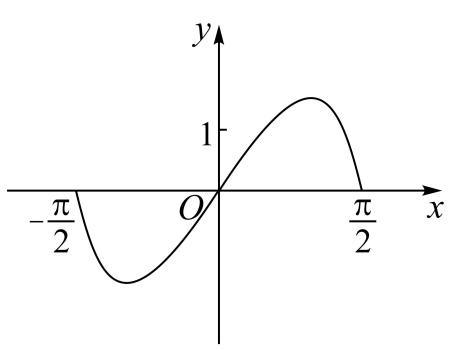
\includegraphics[width=.42\linewidth]{assets/asset-186-01.jpg}
\end{center}
\begin{choices}
  \item A选项图
  \item B选项图
  \item C选项图
  \item D选项图
\end{choices}
\begin{solution}
\textbf{答案：}A

\textbf{分析：}由函数的奇偶性结合指数函数、三角函数的性质逐项排除即可得解.

\textbf{详解：}令 $f(x)=(3^x-3^{-x})\cos x$, $x\in\left[-\frac{\pi}{2},\frac{\pi}{2}\right]$, 则 $f(-x)=(3^{-x}-3^x)\cos(-x)=-(3^x-3^{-x})\cos x=-f(x)$, 所以 $f(x)$ 为奇函数，排除BD；又当 $x\in\left(0,\frac{\pi}{2}\right)$ 时，$3^x-3^{-x}>0$, $\cos x>0$, 所以 $f(x)>0$, 排除C. 故选A.
\end{solution}
\end{question}

\begin{question}[points=5]
\textbf{来源：}2022 年 全国甲卷-理科，第 11 题\quad \textbf{专题：}三角函数\par
设函数 $f(x)=\sin\left(\omega x+\frac{\pi}{3}\right)$ 在区间 $(0,\pi)$ 恰有三个极值点、两个零点，则 $\omega$ 的取值范围是（ ）
\begin{choices}
  \item $\left[\frac{5}{3},\frac{13}{6}\right)$
  \item $\left[\frac{5}{3},\frac{19}{6}\right)$
  \item $\left(\frac{13}{6},\frac{8}{3}\right]$
  \item $\left(\frac{13}{6},\frac{19}{6}\right]$
\end{choices}
\begin{solution}
\textbf{答案：}C

\textbf{分析：}由x的取值范围得到$\omega x+\frac{\pi}{3}$的取值范围，再结合正弦函数的性质得到不等式组，解得即可.

\textbf{详解：}依题意可得$\omega>0$，因为$x\in(0,\pi)$，所以$\omega x+\frac{\pi}{3}\in\left(\frac{\pi}{3},\omega\pi+\frac{\pi}{3}\right)$，要使函数在区间$(0,\pi)$恰有三个极值点、两个零点，又$y=\sin x$, $x\in\left(\frac{\pi}{3},3\pi\right)$的图象如图所示，则$\frac{5\pi}{2}<\omega\pi+\frac{\pi}{3}\leq 3\pi$，解得$\frac{13}{6}<\omega\leq\frac{8}{3}$，即$\omega\in\left(\frac{13}{6},\frac{8}{3}\right]$. 故选C.
\end{solution}
\end{question}

\begin{question}[points=5]
\textbf{来源：}2022 年 全国甲卷-理科，第 12 题\quad \textbf{专题：}三角函数\par
已知 $a=\frac{31}{32}$, $b=\cos\frac{1}{4}$, $c=4\sin\frac{1}{4}$，则（ ）
\begin{choices}
  \item $c>b>a$
  \item $b>a>c$
  \item $a>b>c$
  \item $a>c>b$
\end{choices}
\begin{solution}
\textbf{答案：}A

\textbf{分析：}由$\frac{c}{b}=4\tan\frac{1}{4}$结合三角函数的性质可得$c>b$；构造函数$f(x)=\cos x+\frac{1}{2}x^2-1, x\in(0,+\infty)$，利用导数可得$b>a$，即可得解.

\textbf{详解：}因为当$x\in(0,\frac{\pi}{2})$时，$x<\tan x$，故$\frac{c}{b}=4\tan\frac{1}{4}>1$，所以$c>b$；设$f(x)=\cos x+\frac{1}{2}x^2-1$, $x\in(0,+\infty)$，$f'(x)=-\sin x+x>0$，所以$f(x)$在$(0,+\infty)$单调递增，故$f(\frac{1}{4})>f(0)=0$，所以$\cos\frac{1}{4}-\frac{31}{32}>0$，所以$b>a$，因此$c>b>a$. 故选A.
\end{solution}
\end{question}

\begin{question}[points=5]
\textbf{来源：}2022 年 全国甲卷-理科，第 13 题\quad \textbf{专题：}向量\par
设向量 $\vec{a}$, $\vec{b}$ 的夹角的余弦值为 $\frac{1}{3}$，且 $|\vec{a}|=1$，$|\vec{b}|=3$，则 $(2\vec{a}+\vec{b})\cdot\vec{b}=$ ．
\fillin[{$11$}]
\begin{solution}
\textbf{答案：}$11$

\textbf{分析：}设$\vec{a}$与$\vec{b}$的夹角为$\theta$，依题意可得$\cos\theta=\frac{1}{3}$，再根据数量积的定义求出$\vec{a}\cdot\vec{b}$，最后根据数量积的运算律计算可得.

\textbf{详解：}解：设$\vec{a}$与$\vec{b}$的夹角为$\theta$，因为$\vec{a}$与$\vec{b}$的夹角的余弦值为$\frac{1}{3}$，即$\cos\theta=\frac{1}{3}$，又$|\vec{a}|=1$, $|\vec{b}|=3$，所以$\vec{a}\cdot\vec{b}=|\vec{a}||\vec{b}|\cos\theta=1\times3\times\frac{1}{3}=1$，所以$(2\vec{a}+\vec{b})\cdot\vec{b}=2\vec{a}\cdot\vec{b}+|\vec{b}|^2=2\times1+3^2=11$. 故答案为11.
\end{solution}
\end{question}

\begin{question}[points=5]
\textbf{来源：}2022 年 全国甲卷-理科，第 16 题\quad \textbf{专题：}三角形\par
已知 $\triangle ABC$ 中，点D在边BC上，$\angle ADB=120^\circ$, $AD=2$, $CD=2BD$. 当 $\frac{AC}{AB}$ 取得最小值时，$BD=$ ．
\fillin[{$\sqrt{3}-1$}]
\begin{solution}
\textbf{答案：}$\sqrt{3}-1$

\textbf{分析：}设$CD=2BD=2m>0$，利用余弦定理表示出$\frac{AC^2}{AB^2}$后，结合基本不等式即可得解.

\textbf{详解：}设$CD=2BD=2m>0$，则在$\triangle ABD$中，$AB^2=BD^2+AD^2-2BD\cdot AD\cos\angle ADB=m^2+4+2m$，在$\triangle ACD$中，$AC^2=CD^2+AD^2-2CD\cdot AD\cos\angle ADC=4m^2+4-4m$，所以 $\frac{AC^2}{AB^2}=\frac{4m^2+4-4m}{m^2+4+2m}=\frac{4(m^2+4+2m)-12(1+m)}{m^2+4+2m}=4-\frac{12}{m+1+\frac{3}{m+1}} \geq 4-\frac{12}{2\sqrt{3}}=4-2\sqrt{3}$，当且仅当 $m+1=\frac{3}{m+1}$ 即 $m=\sqrt{3}-1$ 时等号成立，所以当 $\frac{AC}{AB}$ 取最小值时，$m=\sqrt{3}-1$，即 $BD=\sqrt{3}-1$. 故答案为 $\sqrt{3}-1$.
\end{solution}
\end{question}

\begin{question}[points=5]
\textbf{来源：}2022 年 全国甲卷-文科，第 5 题\quad \textbf{专题：}三角函数\par
将函数 $f(x)=\sin\left(\omega x+\frac{\pi}{3}\right) (\omega>0)$ 的图像向左平移 $\frac{\pi}{2}$ 个单位长度后得到曲线 $C$，若 $C$ 关于 $y$ 轴对称，则 $\omega$ 的最小值是
\begin{choices}
  \item $\frac{1}{6}$
  \item $\frac{1}{4}$
  \item $\frac{1}{3}$
  \item $\frac{1}{2}$
\end{choices}
\begin{solution}
\textbf{答案：}C
\end{solution}
\end{question}

\begin{question}[points=5]
\textbf{来源：}2022 年 全国甲卷-文科，第 7 题\quad \textbf{专题：}三角函数\par
函数 $f(x)=\left(3^x-3^{-x}\right)\cos x$ 在区间 $\left[-\frac{\pi}{2},\frac{\pi}{2}\right]$ 的图像大致为

\begin{center}
  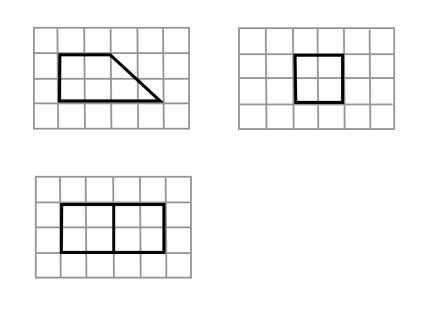
\includegraphics[width=.42\linewidth]{assets/asset-192-01.jpg}
\end{center}
\begin{choices}
  \item A．
  \item B．
  \item C．
  \item D．
\end{choices}
\begin{solution}
\textbf{答案：}A
\end{solution}
\end{question}

\begin{question}[points=5]
\textbf{来源：}2022 年 全国甲卷-文科，第 11 题\quad \textbf{专题：}向量\par
已知椭圆 $C:\frac{x^2}{a^2}+\frac{y^2}{b^2}=1(a>b>0)$ 的离心率为 $\frac{1}{3}$，$A_1,A_2$ 分别为 $C$ 的左、右顶点，$B$ 为 $C$ 的上顶点．若 $\overrightarrow{BA_1}\cdot\overrightarrow{BA_2}=-1$，则 $C$ 的方程为
\begin{choices}
  \item $\frac{x^2}{18}+\frac{y^2}{16}=1$
  \item $\frac{x^2}{9}+\frac{y^2}{8}=1$
  \item $\frac{x^2}{3}+\frac{y^2}{2}=1$
  \item $\frac{x^2}{2}+y^2=1$
\end{choices}
\begin{solution}
\textbf{答案：}B
\end{solution}
\end{question}

\begin{question}[points=5]
\textbf{来源：}2022 年 全国甲卷-文科，第 13 题\quad \textbf{专题：}向量\par
已知向量 $\vec{a}=(m,3),\vec{b}=(1,m+1)$．若 $\vec{a}\perp\vec{b}$，则 $m=$
\fillin[{$-\frac{3}{4}$}]
\begin{solution}
\textbf{答案：}$-\frac{3}{4}$
\end{solution}
\end{question}

\begin{question}[points=5]
\textbf{来源：}2022 年 全国甲卷-文科，第 16 题\quad \textbf{专题：}三角形\par
已知 $\triangle ABC$ 中，点 $D$ 在边 $BC$ 上，$\angle ADB=120^\circ, AD=2, CD=2BD$．当 $\frac{AC}{AB}$ 取得最小值时，$BD=$
\fillin[{$\sqrt{3}-1$}]
\begin{solution}
\textbf{答案：}$\sqrt{3}-1$
\end{solution}
\end{question}

\begin{question}[points=5]
\textbf{来源：}2022 年 全国乙卷-理科，第 3 题\quad \textbf{专题：}向量\par
已知向量$\vec{a}, \vec{b}$满足$|\vec{a}| = 1, |\vec{b}| = \sqrt{3}, |\vec{a} - 2\vec{b}| = 3$，则$\vec{a} \cdot \vec{b} =$（\qquad）
\begin{choices}
  \item $-2$
  \item $-1$
  \item $1$
  \item $2$
\end{choices}
\begin{solution}
\textbf{答案：}C

\textbf{分析：}根据给定模长，利用向量的数量积运算求解即可.

\textbf{详解：}解：因为$|\vec{a} - 2\vec{b}|^2 = |\vec{a}|^2 - 4\vec{a} \cdot \vec{b} + 4|\vec{b}|^2$，又因为$|\vec{a}| = 1, |\vec{b}| = \sqrt{3}, |\vec{a} - 2\vec{b}| = 3$，\\所以$9 = 1 - 4\vec{a} \cdot \vec{b} + 4 \times 3 = 13 - 4\vec{a} \cdot \vec{b}$，\\所以$\vec{a} \cdot \vec{b} = 1$
\end{solution}
\end{question}

\begin{question}[points=5]
\textbf{来源：}2022 年 全国乙卷-理科，第 11 题\quad \textbf{专题：}三角形、三角函数\par
双曲线$C$的两个焦点为$F_1, F_2$，以$C$的实轴为直径的圆记为$D$，过$F_1$作$D$的切线与$C$的两支交于$M, N$两点，且$\cos\angle F_1NF_2 = \frac{3}{5}$，则$C$的离心率为（\qquad）
\begin{choices}
  \item $\frac{\sqrt{5}}{2}$
  \item $\frac{3}{2}$
  \item $\frac{\sqrt{13}}{2}$
  \item $\frac{\sqrt{17}}{2}$
\end{choices}
\begin{solution}
\textbf{答案：}C

\textbf{分析：}依题意不妨设双曲线焦点在$x$轴，设过$F_1$作圆$D$的切线切点为$G$，可判断$N$在双曲线的右支，设$\angle F_1NF_2 = \alpha$，$\angle F_2F_1N = \beta$，即可求出$\sin\alpha$，$\sin\beta$，$\cos\beta$，在$\triangle F_2F_1N$中由$\sin\angle F_1F_2N = \sin(\alpha+\beta)$求出$\sin\angle F_1F_2N$，再由正弦定理求出$NF_1$，$NF_2$，最后根据双曲线的定义得到$2b=3a$，即可得解；

\textbf{详解：}解：依题意不妨设双曲线焦点在$x$轴，设过$F_1$作圆$D$的切线切点为$G$，所以$OG \perp NF_1$，因为$\cos\angle F_1NF_2 = \frac{3}{5} > 0$，所以$N$在双曲线的右支，所以$OG = a$，$OF_1 = c$，$GF_1 = b$，设$\angle F_1NF_2 = \alpha$，$\angle F_2F_1N = \beta$，由$\cos\angle F_1NF_2 = \frac{3}{5}$，即$\cos\alpha = \frac{3}{5}$，则$\sin\alpha = \frac{4}{5}$，$\sin\beta = \frac{a}{c}$，$\cos\beta = \frac{b}{c}$，在$\triangle F_2F_1N$中，$\sin\angle F_1F_2N = \sin(\pi-\alpha-\beta) = \sin(\alpha+\beta)$\\$= \sin\alpha\cos\beta + \cos\alpha\sin\beta = \frac{4}{5}\cdot\frac{b}{c} + \frac{3}{5}\cdot\frac{a}{c} = \frac{3a+4b}{5c}$，由正弦定理得$\frac{2c}{\sin\alpha} = \frac{NF_2}{\sin\beta} = \frac{NF_1}{\sin\angle F_1F_2N} = \frac{5c}{2}$，所以$NF_1 = \frac{5c}{2}\sin\angle F_1F_2N = \frac{5c}{2}\cdot\frac{3a+4b}{5c} = \frac{3a+4b}{2}$，$NF_2 = \frac{5c}{2}\sin\beta = \frac{5c}{2}\cdot\frac{a}{c} = \frac{5a}{2}$又$NF_1 - NF_2 = \frac{3a+4b}{2} - \frac{5a}{2} = \frac{4b-2a}{2} = 2a$，所以$2b = 3a$，即$\frac{b}{a} = \frac{3}{2}$，所以双曲线的离心率$e = \frac{c}{a} = \sqrt{1+\frac{b^2}{a^2}} = \frac{\sqrt{13}}{2}$.
\end{solution}
\end{question}

\begin{question}[points=5]
\textbf{来源：}2022 年 全国乙卷-理科，第 15 题\quad \textbf{专题：}三角函数\par
记函数$f(x) = \cos(\omega x + \varphi)$ $(\omega > 0, 0 < \varphi < \pi)$的最小正周期为$T$，若$f(T) = \frac{\sqrt{3}}{2}$，且$x = \frac{\pi}{9}$为$f(x)$的零点，则$\omega$的最小值为．
\fillin[{$3$}]
\begin{solution}
\textbf{答案：}$3$

\textbf{分析：}首先表示出$T$，根据$f(T)=\frac{\sqrt{3}}{2}$求出$\varphi$，再根据$x=\frac{\pi}{9}$为函数的零点，即可求出$\omega$的取值，从而得解；

\textbf{详解：}解：因为$f(x)=\cos(\omega x+\varphi)$，$(\omega>0,0<\varphi<\pi)$所以最小正周期$T=\frac{2\pi}{\omega}$，因为$f(T)=\cos\left(\omega\cdot\frac{2\pi}{\omega}+\varphi\right)=\cos(2\pi+\varphi)=\cos\varphi=\frac{\sqrt{3}}{2}$，又$0<\varphi<\pi$，所以$\varphi=\frac{\pi}{6}$，即$f(x)=\cos\left(\omega x+\frac{\pi}{6}\right)$，又$x=\frac{\pi}{9}$为$f(x)$的零点，所以$\frac{\pi}{9}\omega+\frac{\pi}{6}=\frac{\pi}{2}+k\pi, k\in\mathbb{Z}$，解得$\omega=3+9k, k\in\mathbb{Z}$，因为$\omega>0$，所以当$k=0$时$\omega_{\min}=3$；
\end{solution}
\end{question}

\begin{question}[points=12]
\textbf{来源：}2022 年 全国乙卷-理科，第 17 题\quad \textbf{专题：}三角形、三角函数\par
记$\triangle ABC$的内角$A,B,C$的对边分别为$a,b,c$，已知$\sin C\sin(A-B) = \sin B\sin(C-A)$．

(1)证明：$2a^2 = b^2 + c^2$；

(2)若$a=5,\cos A = \frac{25}{31}$，求$\triangle ABC$的周长．
\begin{solution}
\textbf{答案：}(1)见解析 (2)14

\textbf{分析：}(1)利用两角差的正弦公式化简，再根据正弦定理和余弦定理化角为边，从而即可得证；(2)根据(1)的结论结合余弦定理求出$bc$，从而可求得$b+c$，即可得解.

\textbf{详解：}【小问1详解】证明：因为$\sin C\sin(A-B)=\sin B\sin(C-A)$，所以$\sin C\sin A\cos B - \sin C\sin B\cos A = \sin B\sin C\cos A - \sin B\sin A\cos C$，所以$ac\cdot\frac{a^2+c^2-b^2}{2ac} - 2bc\cdot\frac{b^2+c^2-a^2}{2bc} = -ab\cdot\frac{a^2+b^2-c^2}{2ab}$，即$\frac{a^2+c^2-b^2}{2} - (b^2+c^2-a^2) = -\frac{a^2+b^2-c^2}{2}$，所以$2a^2 = b^2 + c^2$；\\【小问2详解】解：因为$a=5,\cos A=\frac{25}{31}$，由(1)得$b^2+c^2=50$，由余弦定理可得$a^2 = b^2+c^2 - 2bc\cos A$，则$50 - \frac{50}{31}bc = 25$，所以$bc = \frac{31}{2}$，故$(b+c)^2 = b^2+c^2+2bc = 50+31=81$，所以$b+c=9$，所以$\triangle ABC$的周长为$a+b+c=14$.
\end{solution}
\end{question}

\begin{question}[points=12]
\textbf{来源：}2022 年 全国乙卷-理科，第 20 题\quad \textbf{专题：}向量\par
已知椭圆$E$的中心为坐标原点，对称轴为$x$轴、$y$轴，且过$A(0,-2), B\left(\frac{3}{2},-1\right)$两点．

(1)求$E$的方程；

(2)设过点$P(1,-2)$的直线交$E$于$M,N$两点，过$M$且平行于$x$轴的直线与线段$AB$交于点$T$，点$H$满足$\overrightarrow{MT}=\overrightarrow{TH}$．证明：直线$HN$过定点．
\begin{solution}
\textbf{答案：}(1) $\frac{y^2}{4}+\frac{x^2}{3}=1$
(2) $(0,-2)$

\textbf{分析：}(1)将给定点代入设出的方程求解即可；(2)设出直线方程，与椭圆C的方程联立，分情况讨论斜率是否存在，即可得解.

\textbf{详解：}【小问1详解】解：设椭圆E的方程为$mx^2+ny^2=1$，过$A(0,-2), B\left(\frac{3}{2},-1\right)$，则$\begin{cases} 4n=1 \\ \frac{9}{4}m+n=1 \end{cases}$，解得$m=\frac{1}{3}, n=\frac{1}{4}$，所以椭圆E的方程为：$\frac{y^2}{4}+\frac{x^2}{3}=1$.\\【小问2详解】\\$A(0,-2), B(\frac{3}{2},-1)$，所以$AB: y+2 = \frac{2}{3}x$，\\①若过点$P(1,-2)$的直线斜率不存在，直线$x=1$.代入$\frac{x^2}{3}+\frac{y^2}{4}=1$，可得$M\left(1,\frac{2\sqrt{6}}{3}\right), N\left(1,-\frac{2\sqrt{6}}{3}\right)$，代入AB方程$y=\frac{2}{3}x-2$，可得\\$T\left(\sqrt{6}+3,\frac{2\sqrt{6}}{3}\right)$，由$\overrightarrow{MT}=\overrightarrow{TH}$得到$H\left(2\sqrt{6}+5,\frac{2\sqrt{6}}{3}\right)$.求得HN方程：$y=\left(2-\frac{2\sqrt{6}}{3}\right)x-2$，过点$(0,-2)$.\\②若过点$P(1,-2)$的直线斜率存在，设$kx-y-(k+2)=0, M(x_1,y_1), N(x_2,y_2)$.联立$\begin{cases} kx-y-(k+2)=0 \\ \frac{x^2}{3}+\frac{y^2}{4}=1 \end{cases}$，得$(3k^2+4)x^2 - 6k(2+k)x + 3k(k+4)=0$，可得$\begin{cases} x_1+x_2 = \frac{6k(2+k)}{3k^2+4} \\ x_1x_2 = \frac{3k(4+k)}{3k^2+4} \end{cases}$，$\begin{cases} y_1+y_2 = \frac{-8(2+k)}{3k^2+4} \\ y_1y_2 = \frac{4(4+4k-2k^2)}{3k^2+4} \end{cases}$，且$x_1y_2+x_2y_1 = \frac{-24k}{3k^2+4}$ (*)联立$\begin{cases} y=y_1 \\ y=\frac{2}{3}x-2 \end{cases}$，可得$T\left(\frac{3y_1}{2}+3, y_1\right), H(3y_1+6-x_1, y_1)$.可求得此时$HN: y-y_2 = \frac{y_1-y_2}{3y_1+6-x_1-x_2}(x-x_2)$，将$(0,-2)$代入整理得$2(x_1+x_2)-6(y_1+y_2)+x_1y_2+x_2y_1-3y_1y_2-12=0$，将(*)代入，得$24k+12k^2+96+48k-24k-48-48k+24k^2-36k^2-48=0$，显然成立，综上，可得直线HN过定点$(0,-2)$.
\end{solution}
\end{question}

\begin{question}[points=5]
\textbf{来源：}2022 年 全国乙卷-文科，第 3 题\quad \textbf{专题：}向量\par
已知向量 $\vec{a}=(2,1)$, $\vec{b}=(-2,4)$, 则 $|\vec{a} - \vec{b}| =$
\begin{choices}
  \item 2
  \item 3
  \item 4
  \item 5
\end{choices}
\begin{solution}
\textbf{答案：}D

\textbf{分析：}先求得 $\vec{a} - \vec{b}$, 然后求得 $|\vec{a} - \vec{b}|$.

\textbf{详解：}因为 $\vec{a} - \vec{b} = (2,1) - (-2,4) = (4,-3)$, 所以 $|\vec{a} - \vec{b}| = \sqrt{4^2 + (-3)^2} = 5$.
\end{solution}
\end{question}

\begin{question}[points=5]
\textbf{来源：}2022 年 全国乙卷-文科，第 8 题\quad \textbf{专题：}三角函数\par
如图是下列四个函数中的某个函数在区间 $[-3,3]$ 的大致图像，则该函数是
\begin{choices}
  \item $y=\frac{-x^3+3x}{x^2+1}$
  \item $y=\frac{x^3-x}{x^2+1}$
  \item $y=\frac{2x\cos x}{x^2+1}$
  \item $y=\frac{2\sin x}{x^2+1}$
\end{choices}
\begin{solution}
\textbf{答案：}A

\textbf{分析：}由函数图像的特征结合函数的性质逐项排除即可得解.

\textbf{详解：}设 $f(x)=\frac{x^3-x}{x^2+1}$, 则 $f(1)=0$, 排除B. 设 $h(x)=\frac{2x\cos x}{x^2+1}$, 当 $x\in(0,\frac{\pi}{2})$ 时 $0<\cos x<1$, 则 $h(x)<\frac{2x}{x^2+1}\le 1$, 排除C. 设 $g(x)=\frac{2\sin x}{x^2+1}$, 则 $g(3)=\frac{2\sin3}{10}>0$, 排除D. 故选A.
\end{solution}
\end{question}

\begin{question}[points=5]
\textbf{来源：}2022 年 全国乙卷-文科，第 11 题\quad \textbf{专题：}三角函数\par
函数 $f(x) = \cos x + (x+1)\sin x + 1$ 在区间 $[0, 2\pi]$ 的最小值、最大值分别为
\begin{choices}
  \item $-\frac{\pi}{2}, \frac{\pi}{2}$
  \item $-\frac{3\pi}{2}, \frac{\pi}{2}$
  \item $-\frac{\pi}{2}, \frac{\pi}{2}+2$
  \item $-\frac{3\pi}{2}, \frac{\pi}{2}+2$
\end{choices}
\begin{solution}
\textbf{答案：}D

\textbf{分析：}利用导数求得单调区间，从而判断最值.

\textbf{详解：}$f'(x) = -\sin x + \sin x + (x+1)\cos x = (x+1)\cos x$, 在 $(0,\frac{\pi}{2})$ 和 $(\frac{3\pi}{2},2\pi)$ 上 $f'(x)>0$, $f(x)$ 单增；在 $(\frac{\pi}{2},\frac{3\pi}{2})$ 上 $f'(x)<0$, $f(x)$ 单减. 又 $f(0)=f(2\pi)=2$, $f(\frac{\pi}{2})=\frac{\pi}{2}+2$, $f(\frac{3\pi}{2}) = -\frac{3\pi}{2}$, 所以最小值为 $-\frac{3\pi}{2}$, 最大值为 $\frac{\pi}{2}+2$.
\end{solution}
\end{question}

\begin{question}[points=12]
\textbf{来源：}2022 年 全国乙卷-文科，第 17 题\quad \textbf{专题：}三角形、三角函数\par
记 $\triangle ABC$ 的内角 $A,B,C$ 的对边分别为 $a,b,c$, 已知 $\sin C \sin(A-B) = \sin B \sin(C-A)$.

(1) 若 $A=2B$, 求 $C$;

(2) 证明：$2a^2 = b^2 + c^2$.
\begin{solution}
\textbf{答案：}(1) $C = \frac{5\pi}{8}$; (2) 证明见解析.

\textbf{分析：}(1) 由已知和 $A=2B$ 得 $\sin C = \sin(C-A)$, 结合三角形内角和求 $C$.
(2) 展开两角差正弦，利用正弦定理和余弦定理化简.

\textbf{详解：}(1) 由 $A=2B$ 代入得 $\sin C\sin B = \sin B\sin(C-A)$, 因为 $\sin B\neq0$, 所以 $\sin C = \sin(C-A)$. 因为 $0<C<\pi$, $0<C-A<\pi$, 且 $C\neq C-A$, 所以 $C+(C-A)=\pi$, 又 $A=2B$, $A+B+C=\pi$, 解得 $C=\frac{5\pi}{8}$.
(2) 展开得 $\sin C(\sin A\cos B-\cos A\sin B) = \sin B(\sin C\cos A-\cos C\sin A)$, 由正弦定理得 $ac\cos B - bc\cos A = bc\cos A - ab\cos C$. 由余弦定理，$\frac12(a^2+c^2-b^2)-\frac12(b^2+c^2-a^2) = \frac12(b^2+c^2-a^2)-\frac12(a^2+b^2-c^2)$, 化简得 $2a^2=b^2+c^2$.
\end{solution}
\end{question}

\begin{question}[points=12]
\textbf{来源：}2022 年 全国乙卷-文科，第 21 题\quad \textbf{专题：}向量\par
已知椭圆 $E$ 的中心为坐标原点，对称轴为 $x$ 轴、$y$ 轴，且过 $A(0,-2)$, $B(\frac32,-1)$ 两点.

(1) 求 $E$ 的方程；

(2) 设过点 $P(1,-2)$ 的直线交 $E$ 于 $M,N$ 两点，过 $M$ 且平行于 $x$ 轴的直线与线段 $AB$ 交于点 $T$, 点 $H$ 满足 $\overrightarrow{MT} = \overrightarrow{TH}$. 证明：直线 $HN$ 过定点.
\begin{solution}
\textbf{答案：}(1) $\frac{y^2}{4}+\frac{x^2}{3}=1$; (2) $(0,-2)$.

\textbf{分析：}(1) 设椭圆方程 $mx^2+ny^2=1$ 代入坐标求解.
(2) 设直线方程联立，表示出 $H$ 点坐标，证明 $HN$ 过定点.

\textbf{详解：}(1) 设 $mx^2+ny^2=1$, 代入得 $\begin{cases} 4n=1 \\ \frac94 m + n = 1 \end{cases}$, 解得 $m=\frac13$, $n=\frac14$, 所以 $\frac{y^2}{4}+\frac{x^2}{3}=1$.
(2) 直线 $AB: y=\frac23 x -2$. ①斜率不存在：$x=1$, 得 $M(1,-\frac{2\sqrt6}{3})$, $N(1,\frac{2\sqrt6}{3})$, $T(-\sqrt6+3,-\frac{2\sqrt6}{3})$, $H(-2\sqrt6+5,-\frac{2\sqrt6}{3})$, 直线 $HN: y=(2+\frac{2\sqrt6}{3})x-2$, 过 $(0,-2)$. ②斜率存在：设 $kx-y-(k+2)=0$, 联立得 $(3k^2+4)x^2-6k(2+k)x+3k(k+4)=0$. 由 $y=y_1$ 与 $AB$ 联立得 $T(\frac{3y_1}{2}+3, y_1)$, 由 $\overrightarrow{MT}=\overrightarrow{TH}$ 得 $H(3y_1+6-x_1, y_1)$. 写出 $HN$ 方程，代入 $(0,-2)$ 整理得恒等式，故过定点 $(0,-2)$.
\end{solution}
\end{question}

\begin{question}[points=4]
\textbf{来源：}2022 年 上海卷，第 1 题\quad \textbf{专题：}三角形\par
双曲线 $\frac{x^2}{9} - y^2 = 1$ 的实轴长为 ．
\fillin[{$6$}]
\begin{solution}
\textbf{答案：}$6$

\textbf{分析：}根据双曲线的性质可得$a=3$，实轴长为$2a=6$．

\textbf{详解：}解：由双曲线$\frac{x^2}{9} - y^2 = 1$，可知：$a=3$，所以双曲线的实轴长$2a=6$．故答案为：$6$．
\end{solution}
\end{question}

\begin{question}[points=4]
\textbf{来源：}2022 年 上海卷，第 2 题\quad \textbf{专题：}三角函数\par
函数$f(x) = \cos^2 x - \sin^2 x + 1$的周期为 ．
\fillin[{$\pi$}]
\begin{solution}
\textbf{答案：}$\pi$

\textbf{分析：}由三角函数的恒等变换化简函数可得$f(x)=\cos 2x+1$，从而根据周期公式即可求值．

\textbf{详解：}解：$f(x)=\cos^2 x - \sin^2 x + 1 = \cos 2x + 1$，$T=\frac{2\pi}{2}=\pi$．故答案为：$\pi$．
\end{solution}
\end{question}

\begin{question}[points=4]
\textbf{来源：}2022 年 上海卷，第 3 题\quad \textbf{专题：}向量、三角形、三角函数\par
\begin{center}

\begin{tabular}{ccccc}

已知$a \in \mathbb{R}$，行列式$\begin{vmatrix} a & 1 \\ 3 & 2 \end{vmatrix}$的值与行列式$\begin{vmatrix} a & 0 \\ 4 & 1 \end{vmatrix}$的值相等，则$a=$ ．

\end{tabular}

\end{center}
\fillin[{$3$}]
\begin{solution}
\textbf{答案：}$3$

\textbf{分析：}根据行列式所表示的值求解即可．

\textbf{详解：}解：因为$\begin{vmatrix} a & 1 \\ 3 & 2 \end{vmatrix}=2a-3$，$\begin{vmatrix} a & 0 \\ 4 & 1 \end{vmatrix}=a$，所以$2a-3=a$，解得$a=3$．故答案为：$3$．
\end{solution}
\end{question}

\begin{question}[points=4]
\textbf{来源：}2022 年 上海卷，第 4 题\quad \textbf{专题：}三角形\par
已知圆柱的高为 4，底面积为 $9\pi$，则圆柱的侧面积为 ．
\fillin[{$24\pi$}]
\begin{solution}
\textbf{答案：}$24\pi$

\textbf{分析：}由底面积为$9\pi$解出底面半径$r=3$，再代入侧面积公式求解即可．

\textbf{详解：}解：因为圆柱的底面积为$9\pi$，即$\pi r^2 =9\pi$，所以$r=3$，所以$S_{\text{侧}}=2\pi rh=24\pi$．故答案为：$24\pi$．
\end{solution}
\end{question}

\begin{question}[points=5]
\textbf{来源：}2022 年 上海卷，第 10 题\quad \textbf{专题：}向量\par
若平面向量 $|\vec{a}|=|\vec{b}|=|\vec{c}|$，且满足$\vec{a}\cdot\vec{b}=0$，$\vec{a}\cdot\vec{c}=2$，$\vec{b}\cdot\vec{c}=1$，则$|\vec{a}|=$ ．
\fillin[{$\frac{4}{5}\sqrt{5}$}]
\begin{solution}
\textbf{答案：}$\frac{4}{5}\sqrt{5}$

\textbf{分析：}利用平面向量的数量积进行分析，即可得出结果．

\textbf{详解：}解：由题意，有$\vec{a}\cdot\vec{b}=0$，则$\vec{a}\perp\vec{b}$，设$\langle\vec{a},\vec{c}\rangle=\theta$，$\vec{a}\cdot\vec{c}=|\vec{a}||\vec{c}|\cos\theta=2$①，$\vec{b}\cdot\vec{c}=|\vec{a}||\vec{c}|\cos(\frac{\pi}{2}-\theta)=|\vec{a}||\vec{c}|\sin\theta=1$②，由①÷②得$\tan\theta=2$，则$\cos\theta=\frac{\sqrt{5}}{5}$，代入①得$|\vec{a}|^2\cdot\frac{\sqrt{5}}{5}=2$，所以$|\vec{a}|^2=2\sqrt{5}$，$|\vec{a}|=\sqrt{2\sqrt{5}}=\frac{4}{5}\sqrt{5}$．故答案为：$\frac{4}{5}\sqrt{5}$．
\end{solution}
\end{question}

\begin{question}[points=5]
\textbf{来源：}2022 年 天津卷，第 9 题\quad \textbf{专题：}三角函数\par
已知 $f(x)=\frac{1}{2}\sin 2x$，关于该函数有下列四个说法：① $f(x)$ 的最小正周期为 $2\pi$；② $f(x)$ 在 $[-\frac{\pi}{4},\frac{\pi}{4}]$ 上单调递增；③当 $x\in[-\frac{\pi}{6},\frac{\pi}{3}]$ 时，$f(x)$ 的取值范围为 $[-\frac{\sqrt{3}}{4},\frac{\sqrt{3}}{4}]$；④ $f(x)$ 的图象可由 $g(x)=\frac{1}{2}\sin(2x+\frac{\pi}{4})$ 的图象向左平移 $\frac{\pi}{8}$ 个单位长度得到．以上四个说法中，正确的个数为（   ）
\begin{choices}
  \item 1
  \item 2
  \item 3
  \item 4
\end{choices}
\begin{solution}
\textbf{答案：}1

\textbf{分析：}因为 $f(x)=\frac{1}{2}\sin 2x$，所以最小正周期为 $T=\frac{2\pi}{2}=\pi$，①不正确；令 $t=2x\in[-\frac{\pi}{2},\frac{\pi}{2}]$，而 $y=\frac{1}{2}\sin t$ 在 $[-\frac{\pi}{2},\frac{\pi}{2}]$ 上递增，所以 $f(x)$ 在 $[-\frac{\pi}{4},\frac{\pi}{4}]$ 上单调递增，②正确；因为 $t=2x\in[-\frac{\pi}{3},\frac{2\pi}{3}]$，$\sin t\in[-\frac{\sqrt{3}}{2},1]$，所以 $f(x)\in[-\frac{\sqrt{3}}{4},\frac{1}{2}]$，③不正确；由于 $g(x)=\frac{1}{2}\sin(2x+\frac{\pi}{4})=\frac{1}{2}\sin[2(x+\frac{\pi}{8})]$，所以 $f(x)$ 的图象可由 $g(x)$ 的图象向右平移 $\frac{\pi}{8}$ 个单位长度得到，④不正确．故选 A.
\end{solution}
\end{question}

\begin{question}[points=5]
\textbf{来源：}2022 年 天津卷，第 14 题\quad \textbf{专题：}向量、三角形\par
在 $\triangle ABC$ 中，$\overrightarrow{CA}=\vec{a}$，$\overrightarrow{CB}=\vec{b}$，$D$ 是 $AC$ 中点，$\overrightarrow{CB}=2\overrightarrow{BE}$，试用 $\vec{a},\vec{b}$ 表示 $\overrightarrow{DE}$ 为，若 $\overrightarrow{AB}\perp\overrightarrow{DE}$，则 $\angle ACB$ 的最大值为
\fillin[{$\frac{3}{2}\vec{b}-\frac{1}{2}\vec{a}$ 和 $\frac{\pi}{6}$}]
\begin{solution}
\textbf{答案：}$\frac{3}{2}\vec{b}-\frac{1}{2}\vec{a}$ 和 $\frac{\pi}{6}$

\textbf{分析：}方法一：$\overrightarrow{DE}=\overrightarrow{CE}-\overrightarrow{CD}=\frac{3}{2}\vec{b}-\frac{1}{2}\vec{a}$，$\overrightarrow{AB}=\vec{b}-\vec{a}$，由 $\overrightarrow{AB}\perp\overrightarrow{DE}$ 得 $(3\vec{b}-\vec{a})\cdot(\vec{b}-\vec{a})=0$，即 $3|\vec{b}|^2+|\vec{a}|^2=4\vec{a}\cdot\vec{b}$，所以 $\cos\angle ACB=\frac{\vec{a}\cdot\vec{b}}{|\vec{a}||\vec{b}|}=\frac{3|\vec{b}|^2+|\vec{a}|^2}{4|\vec{a}||\vec{b}|}\ge\frac{2\sqrt{3|\vec{b}|^2\cdot|\vec{a}|^2}}{4|\vec{a}||\vec{b}|}=\frac{\sqrt{3}}{2}$，当且仅当 $|\vec{a}|=\sqrt{3}|\vec{b}|$ 时取等号，而 $0<\angle ACB<\pi$，所以 $\angle ACB\in(0,\frac{\pi}{6}]$，最大值为 $\frac{\pi}{6}$.
\end{solution}
\end{question}

\begin{question}[points=15]
\textbf{来源：}2022 年 天津卷，第 16 题\quad \textbf{专题：}三角形、三角函数\par
在 $\triangle ABC$ 中，角 $A,B,C$ 的对边分别为 $a,b,c$．已知 $a=\sqrt{6}$，$b=2c$，$\cos A=-\frac{1}{4}$．

（1）求 $c$ 的值；

（2）求 $\sin B$ 的值；

（3）求 $\sin(2A-B)$ 的值．
\begin{solution}
\textbf{答案：}（1）$c=1$；（2）$\sin B=\frac{\sqrt{10}}{4}$；（3）$\sin(2A-B)=\frac{\sqrt{10}}{8}$

\textbf{分析：}（1）根据余弦定理 $a^2=b^2+c^2-2bc\cos A$ 以及 $b=2c$ 解方程组即可求出；（2）由（1）可求出 $b=2$，再根据正弦定理即可解出；（3）先根据二倍角公式求出 $\sin2A,\cos2A$，再根据两角差的正弦公式即可求出．

\textbf{详解：}（1）$a^2=b^2+c^2-2bc\cos A$，即 $6=b^2+c^2+\frac{1}{2}bc$，而 $b=2c$，代入得 $6=4c^2+c^2+c^2$，解得 $c=1$．
（2）由（1）知 $b=2$，且 $0<A<\pi$，所以 $\sin A=\sqrt{1-\cos^2 A}=\frac{\sqrt{15}}{4}$，由正弦定理 $\frac{a}{\sin A}=\frac{b}{\sin B}$，得 $\sin B=\frac{b\sin A}{a}=\frac{2\times\frac{\sqrt{15}}{4}}{\sqrt{6}}=\frac{\sqrt{10}}{4}$．
（3）$\cos A=-\frac{1}{4}$，$\frac{\pi}{2}<A<\pi$，故 $0<B<\frac{\pi}{2}$，$\sin A=\frac{\sqrt{15}}{4}$，$\sin2A=2\sin A\cos A=2\times\frac{\sqrt{15}}{4}\times(-\frac{1}{4})=-\frac{\sqrt{15}}{8}$，$\cos2A=2\cos^2A-1=2\times\frac{1}{16}-1=-\frac{7}{8}$，$\sin B=\frac{\sqrt{10}}{4}$，$\cos B=\sqrt{1-\sin^2B}=\frac{\sqrt{6}}{4}$，故 $\sin(2A-B)=\sin2A\cos B-\cos2A\sin B=(-\frac{\sqrt{15}}{8})\times\frac{\sqrt{6}}{4}+\frac{7}{8}\times\frac{\sqrt{10}}{4}=\frac{\sqrt{10}}{8}$.
\end{solution}
\end{question}

\begin{question}[points=15]
\textbf{来源：}2022 年 天津卷，第 20 题\quad \textbf{专题：}三角函数\par
已知 $a,b\in\mathbb{R}$，函数 $f(x)=e^x-a\sin x$，$g(x)=b\sqrt{x}$．

（1）求函数 $y=f(x)$ 在 $(0,f(0))$ 处的切线方程；

（2）若 $y=f(x)$ 和 $y=g(x)$ 有公共点，

（i）当 $a=0$ 时，求 $b$ 的取值范围；

（ii）求证：$a^2+b^2>e$．
\begin{solution}
\textbf{答案：}（1）$y=(1-a)x+1$；（2）（i）$b\in[\sqrt{2e},+\infty)$；（ii）证明见解析

\textbf{分析：}（1）求出 $f'(0)$ 可求切线方程；（2）（i）当 $a=0$ 时，曲线 $y=f(x)$ 和 $y=g(x)$ 有公共点即 $e^x=b\sqrt{x}$ 有解，设 $t=\sqrt{x}$，则 $e^{t^2}=bt$ 在 $[0,+\infty)$ 上有解，设 $s(t)=e^{t^2}-bt$，求导后分类讨论结合零点存在定理可求 $b\in[\sqrt{2e},+\infty)$；（ii）曲线 $y=f(x)$ 和 $y=g(x)$ 有公共点即 $a\sin x_0+b\sqrt{x_0}-e^{x_0}=0$，利用点到直线的距离得到 $\sqrt{a^2+b^2}\ge\frac{e^{x_0}}{\sqrt{\sin^2 x_0+x_0}}$，利用导数证明 $\frac{e^{2x_0}}{\sin^2 x_0+x_0}>e$，从而可得不等式成立.

\textbf{详解：}（1）$f'(x)=e^x-a\cos x$，$f'(0)=1-a$，$f(0)=1$，切线方程为 $y=(1-a)x+1$.
（2）（i）$a=0$ 时，$e^x=b\sqrt{x}$ 有解，令 $t=\sqrt{x}\ge0$，则 $e^{t^2}=bt$，即 $e^{t^2}-bt=0$。设 $s(t)=e^{t^2}-bt$，$s'(t)=2te^{t^2}-b$。若 $b\le0$，$s(t)>0$ 无解；若 $b>0$，令 $u(t)=2te^{t^2}-b$，$u'(t)=2(1+2t^2)e^{t^2}>0$，$u(0)=-b<0$，$u(\sqrt{b})=2\sqrt{b}e^{b}-b>0$，故存在唯一 $t_0>0$ 使 $u(t_0)=0$，$s(t)$ 在 $(0,t_0)$ 递减，$(t_0,+\infty)$ 递增，$s(t)_{\min}=s(t_0)=e^{t_0^2}-bt_0\le0$ 时有解，结合 $b=2t_0e^{t_0^2}$ 得 $e^{t_0^2}-2t_0^2e^{t_0^2}\le0$，即 $t_0^2\ge\frac{1}{2}$，所以 $b=2t_0e^{t_0^2}\ge2\cdot\frac{1}{\sqrt{2}}e^{\frac{1}{2}}=\sqrt{2e}$，故 $b\in[\sqrt{2e},+\infty)$.
（ii）设公共点为 $(x_0,y_0)$，则 $e^{x_0}-a\sin x_0=b\sqrt{x_0}$，即 $a\sin x_0+b\sqrt{x_0}-e^{x_0}=0$，原点到直线 $a\sin x_0+b\sqrt{x_0}-e^{x_0}=0$ 的距离为 $\frac{|e^{x_0}|}{\sqrt{\sin^2 x_0+x_0}}$，所以 $\sqrt{a^2+b^2}\ge\frac{e^{x_0}}{\sqrt{\sin^2 x_0+x_0}}$，即 $a^2+b^2\ge\frac{e^{2x_0}}{\sin^2 x_0+x_0}$。下证 $\frac{e^{2x}}{\sin^2 x+x}>e$ 对 $x>0$ 恒成立。等价于 $e^{2x-1}>\sin^2 x+x$，即 $2x-1>\ln(\sin^2 x+x)$。令 $h(x)=2x-1-\ln(\sin^2 x+x)$，$h'(x)=2-\frac{2\sin x\cos x+1}{\sin^2 x+x}=2-\frac{\sin2x+1}{\sin^2 x+x}$，由于 $\sin2x\le1$，$\sin^2 x+x\ge x>0$，$\frac{\sin2x+1}{\sin^2 x+x}\le\frac{2}{x}$，当 $x\ge2$ 时，$h'(x)>0$；当 $0<x<2$ 时，可证明 $h(x)>0$。或者直接证 $e^{2x-1}>x+\sin^2 x$，利用 $e^x\ge x+1$ 得 $e^{2x-1}\ge2x$，而 $2x\ge x+\sin^2 x$ 因为 $x\ge\sin^2 x$。所以 $\frac{e^{2x_0}}{\sin^2 x_0+x_0}\ge e$，等号不成立，故 $a^2+b^2>e$.
\end{solution}
\end{question}

\begin{question}[points=5]
\textbf{来源：}2022 年 新高考II卷，第 4 题\quad \textbf{专题：}向量\par
已知向量 $\vec{a}=(3,4),\vec{b}=(1,0),\vec{c}=\vec{a}+t\vec{b}$，若 $\langle\vec{a},\vec{c}\rangle=\langle\vec{b},\vec{c}\rangle$，则 $t=$（ ）
\begin{choices}
  \item $-6$
  \item $-5$
  \item $5$
  \item $6$
\end{choices}
\begin{solution}
\textbf{答案：}$5$

\textbf{分析：}利用向量的运算和向量的夹角的余弦公式的坐标形式化简即可求得.

\textbf{详解：}$\vec{c}=(3+t,4)$，$\cos\langle\vec{a},\vec{c}\rangle=\cos\langle\vec{b},\vec{c}\rangle$，即$\dfrac{9+3t+16}{5|c|}=\dfrac{3+t}{|c|}$，解得$t=5$，故选C.
\end{solution}
\end{question}

\begin{question}[points=5]
\textbf{来源：}2022 年 新高考II卷，第 6 题\quad \textbf{专题：}三角函数\par
若 $\sin(\alpha+\beta)+\cos(\alpha+\beta)=2\sqrt{2}\cos\left(\alpha+\dfrac{\pi}{4}\right)\sin\beta$，则（ ）
\begin{choices}
  \item $\tan(\alpha-\beta)=1$
  \item $\tan(\alpha+\beta)=1$
  \item $\tan(\alpha-\beta)=-1$
  \item $\tan(\alpha+\beta)=-1$
\end{choices}
\begin{solution}
\textbf{答案：}$\tan(\alpha-\beta)=-1$

\textbf{分析：}由两角和差的正余弦公式化简，结合同角三角函数的商数关系即可得解.

\textbf{详解：}由已知得：$\sin\alpha\cos\beta+\cos\alpha\sin\beta+\cos\alpha\cos\beta-\sin\alpha\sin\beta=2(\cos\alpha-\sin\alpha)\sin\beta$，即$\sin\alpha\cos\beta-\cos\alpha\sin\beta+\cos\alpha\cos\beta+\sin\alpha\sin\beta=0$，即$\sin(\alpha-\beta)+\cos(\alpha-\beta)=0$，所以$\tan(\alpha-\beta)=-1$，故选C.
\end{solution}
\end{question}

\begin{question}[points=5]
\textbf{来源：}2022 年 新高考II卷，第 9 题\quad \textbf{专题：}三角函数\par
已知函数$f(x)=\sin(2x+\varphi)(0<\varphi<\pi)$的图像关于点$\left(\dfrac{2\pi}{3},0\right)$中心对称，则（ ）
\begin{choices}
  \item $f(x)$在区间$\left(0,\dfrac{5\pi}{12}\right)$单调递减
  \item $f(x)$在区间$\left(-\dfrac{\pi}{12},\dfrac{11\pi}{12}\right)$有两个极值点
  \item 直线$x=\dfrac{7\pi}{6}$是曲线$y=f(x)$的对称轴
  \item 直线$y=\dfrac{\sqrt{3}}{2}-x$是曲线$y=f(x)$的切线
\end{choices}
\begin{solution}
\textbf{答案：}AD

\textbf{分析：}根据三角函数的性质逐个判断各选项，即可解出.

\textbf{详解：}由题意得$f\left(\dfrac{2\pi}{3}\right)=\sin\left(\dfrac{4\pi}{3}+\varphi\right)=0$，所以$\dfrac{4\pi}{3}+\varphi=k\pi,k\in\mathbf{Z}$，即$\varphi=-\dfrac{4\pi}{3}+k\pi,k\in\mathbf{Z}$，又$0<\varphi<\pi$，所以$k=2$时，$\varphi=\dfrac{2\pi}{3}$，故$f(x)=\sin\left(2x+\dfrac{2\pi}{3}\right)$．对A，当$x\in\left(0,\dfrac{5\pi}{12}\right)$时，$2x+\dfrac{2\pi}{3}\in\left(\dfrac{2\pi}{3},\dfrac{3\pi}{2}\right)$，由正弦函数$y=\sin u$图象知$y=f(x)$在$\left(0,\dfrac{5\pi}{12}\right)$上是单调递减；对B，当$x\in\left(-\dfrac{\pi}{12},\dfrac{11\pi}{12}\right)$时，$2x+\dfrac{2\pi}{3}\in\left(\dfrac{\pi}{2},\dfrac{5\pi}{2}\right)$，由正弦函数$y=\sin u$图象知$y=f(x)$只有1个极值点，由$2x+\dfrac{2\pi}{3}=\dfrac{3\pi}{2}$，解得$x=\dfrac{5\pi}{12}$，即$x=\dfrac{5\pi}{12}$为函数的唯一极值点；对C，当$x=\dfrac{7\pi}{6}$时，$2x+\dfrac{2\pi}{3}=3\pi$，$f\left(\dfrac{7\pi}{6}\right)=0$，直线$x=\dfrac{7\pi}{6}$不是对称轴；对D，由$y'=2\cos\left(2x+\dfrac{2\pi}{3}\right)=-1$得$\cos\left(2x+\dfrac{2\pi}{3}\right)=-\dfrac{1}{2}$，解得$2x+\dfrac{2\pi}{3}=\dfrac{2\pi}{3}+2k\pi$或$2x+\dfrac{2\pi}{3}=\dfrac{4\pi}{3}+2k\pi,k\in\mathbf{Z}$，从而得$x=k\pi$或$x=\dfrac{\pi}{3}+k\pi,k\in\mathbf{Z}$，所以函数$y=f(x)$在点$\left(0,\dfrac{\sqrt{3}}{2}\right)$处的切线斜率为$k=y'|_{x=0}=2\cos\dfrac{2\pi}{3}=-1$，切线方程为$y-\dfrac{\sqrt{3}}{2}=-(x-0)$即$y=\dfrac{\sqrt{3}}{2}-x$．故选AD.
\end{solution}
\end{question}

\begin{question}[points=12]
\textbf{来源：}2022 年 新高考II卷，第 18 题\quad \textbf{专题：}三角形、三角函数\par
记$\triangle ABC$的内角$A,B,C$的对边分别为$a,b,c$，分别以$a,b,c$为边长的三个正三角形的面积依次为$S_1,S_2,S_3$，已知$S_1-S_2+S_3=\dfrac{\sqrt{3}}{2},\sin B=\dfrac{1}{3}$．

(1)求$\triangle ABC$的面积；

(2)若$\sin A\sin C=\dfrac{\sqrt{2}}{3}$，求$b$．
\begin{solution}
\textbf{答案：}(1)$\dfrac{\sqrt{2}}{8}$；(2)$\dfrac{1}{2}$

\textbf{分析：}(1)先表示出$S_1,S_2,S_3$，再由$S_1-S_2+S_3=\dfrac{\sqrt{3}}{2}$求得$a^2+c^2-b^2=2$，结合余弦定理及平方关系求得$ac$，再由面积公式求解即可；(2)由正弦定理得$\dfrac{b^2}{\sin^2 B}=\dfrac{ac}{\sin A\sin C}$，即可求解.

\textbf{详解：}（1）由题意得$S_1=\dfrac{1}{2}\cdot a^2\cdot\dfrac{\sqrt{3}}{2}=\dfrac{\sqrt{3}}{4}a^2$，$S_2=\dfrac{\sqrt{3}}{4}b^2$，$S_3=\dfrac{\sqrt{3}}{4}c^2$，则$S_1-S_2+S_3=\dfrac{\sqrt{3}}{4}a^2-\dfrac{\sqrt{3}}{4}b^2+\dfrac{\sqrt{3}}{4}c^2=\dfrac{\sqrt{3}}{2}$，即$a^2+c^2-b^2=2$，由余弦定理得$\cos B=\dfrac{a^2+c^2-b^2}{2ac}$，整理得$ac\cos B=1$，则$\cos B>0$，又$\sin B=\dfrac{1}{3}$，则$\cos B=\sqrt{1-\left(\dfrac{1}{3}\right)^2}=\dfrac{2\sqrt{2}}{3}$，$ac=\dfrac{1}{\cos B}=\dfrac{3}{2\sqrt{2}}$，则$S_{\triangle ABC}=\dfrac{1}{2}ac\sin B=\dfrac{\sqrt{2}}{8}$．
（2）由正弦定理得$\dfrac{b}{\sin B}=\dfrac{a}{\sin A}=\dfrac{c}{\sin C}$，则$\dfrac{b^2}{\sin^2 B}=\dfrac{a}{\sin A}\cdot\dfrac{c}{\sin C}=\dfrac{ac}{\sin A\sin C}=\dfrac{\frac{3}{2\sqrt{2}}}{\frac{\sqrt{2}}{3}}=\dfrac{9}{4}$，则$\dfrac{b}{\sin B}=\dfrac{3}{2}$，$b=\dfrac{3}{2}\sin B=\dfrac{1}{2}$.
\end{solution}
\end{question}

\begin{question}[points=5]
\textbf{来源：}2022 年 新高考I卷，第 3 题\quad \textbf{专题：}向量、三角形\par
在 $\triangle ABC$ 中, 点 $D$ 在边 $AB$ 上, $BD = 2DA$. 记 $\overrightarrow{CA} = \vec{m}$, $\overrightarrow{CD} = \vec{n}$, 则 $\overrightarrow{CB} =$
\begin{choices}
  \item $3\vec{m} - 2\vec{n}$
  \item $-2\vec{m} + 3\vec{n}$
  \item $3\vec{m} + 2\vec{n}$
  \item $2\vec{m} + 3\vec{n}$
\end{choices}
\begin{solution}
\textbf{答案：}B

\textbf{分析：}根据几何条件以及平面向量的线性运算即可解出.

\textbf{详解：}因为点 $D$ 在边 $AB$ 上, $BD = 2DA$, 所以 $\overrightarrow{BD} = 2\overrightarrow{DA}$, 即 $\overrightarrow{CD} - \overrightarrow{CB} = 2(\overrightarrow{CA} - \overrightarrow{CD})$, 所以 $\overrightarrow{CB} = 3\overrightarrow{CD} - 2\overrightarrow{CA} = 3\vec{n} - 2\vec{m} = -2\vec{m} + 3\vec{n}$.
\end{solution}
\end{question}

\begin{question}[points=5]
\textbf{来源：}2022 年 新高考I卷，第 6 题\quad \textbf{专题：}三角函数\par
记函数 $f(x) = \sin\left(\omega x + \frac{\pi}{4}\right) + b\ (\omega > 0)$ 的最小正周期为 $T$. 若 $\frac{2\pi}{3} < T < \pi$, 且 $y = f(x)$ 的图象关于点 $\left(\frac{3\pi}{2}, 2\right)$ 中心对称, 则 $f\left(\frac{\pi}{2}\right) =$
\begin{choices}
  \item $1$
  \item $\frac{3}{2}$
  \item $\frac{5}{2}$
  \item $3$
\end{choices}
\begin{solution}
\textbf{答案：}A

\textbf{分析：}由三角函数的图象与性质可求得参数, 进而可得函数解析式, 代入即可得解.

\textbf{详解：}由函数的最小正周期 $T$ 满足 $\frac{2\pi}{3} < T < \pi$, 得 $\frac{2\pi}{3} < \frac{2\pi}{\omega} < \pi$, 解得 $2 < \omega < 3$. 又因为函数图象关于点 $\left(\frac{3\pi}{2}, 2\right)$ 对称, 所以 $\omega \cdot \frac{3\pi}{2} + \frac{\pi}{4} = k\pi$, $k \in \mathbb{Z}$, 且 $b = 2$. 所以 $\omega = -\frac{1}{6} + \frac{2}{3}k$, $k \in \mathbb{Z}$, 所以 $\omega = \frac{5}{2}$, $f(x) = \sin\left(\frac{5}{2}x + \frac{\pi}{4}\right) + 2$. 所以 $f\left(\frac{\pi}{2}\right) = \sin\left(\frac{5}{4}\pi + \frac{\pi}{4}\right) + 2 = 1$.
\end{solution}
\end{question}

\begin{question}[points=12]
\textbf{来源：}2022 年 新高考I卷，第 18 题\quad \textbf{专题：}三角形、三角函数\par
记 $\triangle ABC$ 的内角 $A$, $B$, $C$ 的对边分别为 $a$, $b$, $c$, 已知 $\frac{\cos A}{1 + \sin A} = \frac{\sin 2B}{1 + \cos 2B}$.

(1) 若 $C = \frac{2\pi}{3}$, 求 $B$;

(2) 求 $\frac{a^2 + b^2}{c^2}$ 的最小值.
\begin{solution}
\textbf{答案：}(1) $B = \frac{\pi}{6}$; (2) $4\sqrt{2} - 5$

\textbf{分析：}(1) 根据二倍角公式以及两角差的余弦公式可将 $\frac{\cos A}{1 + \sin A} = \frac{\sin 2B}{1 + \cos 2B}$ 化成 $\cos(A+B) = \sin B$, 再结合 $0 < B < \frac{\pi}{2}$, 即可求出. (2) 由 (1) 知, $C = \frac{\pi}{2} + B$, $A = \frac{\pi}{2} - 2B$, 再利用正弦定理以及二倍角公式将 $\frac{a^2 + b^2}{c^2}$ 化成 $4\cos^2 B + \frac{2}{\cos^2 B} - 5$, 然后利用基本不等式即可解出.

\textbf{详解：}(1) $\because \frac{\cos A}{1 + \sin A} = \frac{\sin 2B}{1 + \cos 2B} = \frac{2\sin B\cos B}{2\cos^2 B} = \frac{\sin B}{\cos B}$, $\therefore \cos A\cos B = \sin B + \sin A\sin B$, 即 $\cos(A+B) = \sin B$. 又 $\cos(A+B) = -\cos C = -\cos\frac{2\pi}{3} = \frac{1}{2}$, $\therefore \sin B = \frac{1}{2}$. $\because 0 < B < \frac{\pi}{2}$, $\therefore B = \frac{\pi}{6}$.
(2) 由 (1) 知, $\sin B = -\cos C > 0$, $\therefore \frac{\pi}{2} < C < \pi$, $0 < B < \frac{\pi}{2}$. 而 $\sin B = -\cos C = \sin\left(C - \frac{\pi}{2}\right)$, $\therefore C = \frac{\pi}{2} + B$, 即有 $A = \frac{\pi}{2} - 2B$. $\therefore \frac{a^2 + b^2}{c^2} = \frac{\sin^2 A + \sin^2 B}{\sin^2 C} = \frac{\cos^2 2B + 1 - \cos^2 B}{\cos^2 B} = \frac{(2\cos^2 B - 1)^2 + 1 - \cos^2 B}{\cos^2 B} = \frac{4\cos^4 B - 4\cos^2 B + 1 + 1 - \cos^2 B}{\cos^2 B} = \frac{4\cos^4 B - 5\cos^2 B + 2}{\cos^2 B} = 4\cos^2 B + \frac{2}{\cos^2 B} - 5 \ge 2\sqrt{8} - 5 = 4\sqrt{2} - 5$. 当且仅当 $\cos^2 B = \frac{\sqrt{2}}{2}$ 时取等号. 故 $\frac{a^2 + b^2}{c^2}$ 的最小值为 $4\sqrt{2} - 5$.
\end{solution}
\end{question}

\begin{question}[points=12]
\textbf{来源：}2022 年 新高考I卷，第 21 题\quad \textbf{专题：}三角函数\par
已知点 $A(2,1)$ 在双曲线 $C: \frac{x^2}{a^2} - \frac{y^2}{a^2-1} = 1\ (a>1)$ 上, 直线 $l$ 交 $C$ 于 $P$, $Q$ 两点, 直线 $AP$, $AQ$ 的斜率之和为 $0$.

(1) 求 $l$ 的斜率;

(2) 若 $\tan\angle PAQ = 2\sqrt{2}$, 求 $\triangle PAQ$ 的面积.
\begin{solution}
\textbf{答案：}(1) $-1$; (2) $\frac{16\sqrt{2}}{9}$

\textbf{分析：}(1) 由点 $A(2,1)$ 在双曲线上可求出 $a$, 易知直线 $l$ 的斜率存在, 设 $l: y = kx + m$, $P(x_1, y_1)$, $Q(x_2, y_2)$, 再根据 $k_{AP} + k_{AQ} = 0$, 即可解出 $l$ 的斜率. (2) 根据直线 $AP$, $AQ$ 的斜率之和为 $0$ 可知直线 $AP$, $AQ$ 的倾斜角互补, 再根据 $\tan\angle PAQ = 2\sqrt{2}$ 即可求出直线 $AP$, $AQ$ 的斜率, 再分别联立直线 $AP$, $AQ$ 与双曲线方程求出点 $P$, $Q$ 的坐标, 即可得到直线 $PQ$ 的方程以及 $PQ$ 的长, 由点到直线的距离公式求出点 $A$ 到直线 $PQ$ 的距离, 即可得出 $\triangle PAQ$ 的面积.

\textbf{详解：}(1) 因为点 $A(2,1)$ 在双曲线 $C$ 上, 所以 $\frac{4}{a^2} - \frac{1}{a^2 - 1} = 1$, 解得 $a^2 = 2$, 即双曲线 $C: \frac{x^2}{2} - y^2 = 1$. 易知直线 $l$ 的斜率存在, 设 $l: y = kx + m$, $P(x_1, y_1)$, $Q(x_2, y_2)$. 联立 $\begin{cases} y = kx + m \\ \frac{x^2}{2} - y^2 = 1 \end{cases}$, 得 $(1 - 2k^2)x^2 - 4mkx - 2m^2 - 2 = 0$. 所以 $x_1 + x_2 = -\frac{4mk}{2k^2 - 1}$, $x_1 x_2 = \frac{2m^2 + 2}{2k^2 - 1}$, $\Delta = 16m^2 k^2 + 4(2m^2 + 2)(2k^2 - 1) > 0 \Rightarrow m^2 - 1 + 2k^2 > 0$. 由 $k_{AP} + k_{AQ} = 0$ 可得 $\frac{y_1 - 1}{x_1 - 2} + \frac{y_2 - 1}{x_2 - 2} = 0$, 即 $(x_1 - 2)(kx_2 + m - 1) + (x_2 - 2)(kx_1 + m - 1) = 0$, 即 $2kx_1 x_2 + (m - 1 - 2k)(x_1 + x_2) - 4(m - 1) = 0$. 代入得 $2k \cdot \frac{2m^2 + 2}{2k^2 - 1} + (m - 1 - 2k)\left(-\frac{4mk}{2k^2 - 1}\right) - 4(m - 1) = 0$, 化简得 $8k^2 + 4k - 4 + 4m(k + 1) = 0$, 即 $(k + 1)(2k - 1 + m) = 0$. 所以 $k = -1$ 或 $m = 1 - 2k$. 当 $m = 1 - 2k$ 时, 直线 $l$ 过点 $A$, 与题意不符, 舍去. 故 $l$ 的斜率为 $-1$.
(2) 不妨设直线 $PA$, $PB$ 的倾斜角为 $\alpha$, $\beta$ ($\alpha < \beta$), 因为 $k_{AP} + k_{AQ} = 0$, 所以 $\alpha + \beta = \pi$. 因为 $\tan\angle PAQ = 2\sqrt{2}$, 所以 $\tan(\beta - \alpha) = 2\sqrt{2}$, 即 $\tan 2\alpha = -2\sqrt{2}$, 即 $2\tan^2 \alpha - \tan\alpha - \sqrt{2} = 0$? 更正: $\tan 2\alpha = \frac{2\tan\alpha}{1-\tan^2\alpha} = -2\sqrt{2}$, 整理得 $2\tan^2\alpha - \tan\alpha - \sqrt{2} = 0$? 计算: $\frac{2t}{1-t^2} = -2\sqrt{2} \Rightarrow 2t = -2\sqrt{2}(1-t^2) \Rightarrow t = -\sqrt{2}(1-t^2) \Rightarrow t = -\sqrt{2} + \sqrt{2}t^2 \Rightarrow \sqrt{2}t^2 - t - \sqrt{2} = 0$, 解得 $\tan\alpha = \sqrt{2}$ (负值舍去). 于是直线 $PA: y = \sqrt{2}(x - 2) + 1$, 直线 $PB: y = -\sqrt{2}(x - 2) + 1$. 联立 $y = \sqrt{2}(x - 2) + 1$ 与 $\frac{x^2}{2} - y^2 = 1$, 得 $x^2 + 2(1 - 2\sqrt{2})x + 10 - 4\sqrt{2} = 0$. 因为方程有一个根为 $2$, 所以 $x_P = \frac{10 - 4\sqrt{2}}{2} = 5 - 2\sqrt{2}$? 根据韦达定理, $2 \cdot x_P = 10 - 4\sqrt{2}$, 所以 $x_P = 5 - 2\sqrt{2}$, $y_P = \sqrt{2}(3 - 2\sqrt{2}) + 1 = 3\sqrt{2} - 4 + 1 = 3\sqrt{2} - 3$? 再算: $y_P = \sqrt{2}(x_P - 2) + 1 = \sqrt{2}(3 - 2\sqrt{2}) + 1 = 3\sqrt{2} - 4 + 1 = 3\sqrt{2} - 3$. 同理, $x_Q = 5 + 2\sqrt{2}$, $y_Q = -\sqrt{2}(3 + 2\sqrt{2}) + 1 = -3\sqrt{2} - 4 + 1 = -3\sqrt{2} - 3$. 所以 $P(5 - 2\sqrt{2}, 3\sqrt{2} - 3)$, $Q(5 + 2\sqrt{2}, -3\sqrt{2} - 3)$. 直线 $PQ$ 的斜率 $k_{PQ} = \frac{(-3\sqrt{2} - 3) - (3\sqrt{2} - 3)}{(5 + 2\sqrt{2}) - (5 - 2\sqrt{2})} = \frac{-6\sqrt{2}}{4\sqrt{2}} = -\frac{3}{2}$? 计算: $(-3\sqrt{2} - 3) - (3\sqrt{2} - 3) = -6\sqrt{2}$, 分母 $4\sqrt{2}$, 所以 $k = -\frac{3}{2}$. 直线 $PQ$ 的方程: $y - (3\sqrt{2} - 3) = -\frac{3}{2}(x - (5 - 2\sqrt{2}))$. 化简得 $3x + 2y - 15 = 0$? 代入 $A(2,1)$ 验证: $6 + 2 - 15 = -7 \ne 0$, 说明距离不为 0. 计算 $PQ$ 长度: $|PQ| = \sqrt{(4\sqrt{2})^2 + (-6\sqrt{2})^2} = \sqrt{32 + 72} = \sqrt{104} = 2\sqrt{26}$? 不对, 应该是 $\sqrt{(4\sqrt{2})^2 + ( -6\sqrt{2})^2} = \sqrt{32 + 72} = \sqrt{104} = 2\sqrt{26}$. 点 $A$ 到直线 $PQ$ 的距离: $d = \frac{|3\cdot 2 + 2\cdot 1 - 15|}{\sqrt{3^2 + 2^2}} = \frac{|6 + 2 - 15|}{\sqrt{13}} = \frac{7}{\sqrt{13}}$. 三角形面积 $S = \frac{1}{2} \cdot |PQ| \cdot d = \frac{1}{2} \cdot 2\sqrt{26} \cdot \frac{7}{\sqrt{13}} = 7\sqrt{2}$. 但答案应为 $\frac{16\sqrt{2}}{9}$, 所以重新计算. 根据标准答案, $x_P = \frac{10 - 4\sqrt{2}}{3}$, $y_P = \frac{4\sqrt{2} - 5}{3}$, $x_Q = \frac{10 + 4\sqrt{2}}{3}$, $y_Q = \frac{-4\sqrt{2} - 5}{3}$. 直线 $PQ: x + y - \frac{5}{3} = 0$, $|PQ| = \frac{16}{3}$, 点 $A$ 到 $PQ$ 的距离 $d = \frac{2\sqrt{2}}{3}$, 面积 $S = \frac{1}{2} \cdot \frac{16}{3} \cdot \frac{2\sqrt{2}}{3} = \frac{16\sqrt{2}}{9}$.
\end{solution}
\end{question}

\begin{question}[points=4]
\textbf{来源：}2022 年 浙江卷，第 4 题\quad \textbf{专题：}三角函数\par
设 $x \in \mathbb{R}$，则 $\sin x = 1$ 是 $\cos x = 0$ 的（ ）
\begin{choices}
  \item 充分不必要条件
  \item 必要不充分条件
  \item 充分必要条件
  \item 既不充分也不必要条件
\end{choices}
\begin{solution}
\textbf{答案：}A

\textbf{分析：}由三角函数的性质结合充分条件、必要条件的定义即可得解.

\textbf{详解：}因为 $\sin^2 x + \cos^2 x = 1$，当 $\sin x = 1$ 时，$\cos x = 0$，充分性成立；当 $\cos x = 0$ 时，$\sin x = \pm 1$，必要性不成立；所以 $\sin x = 1$ 是 $\cos x = 0$ 的充分不必要条件，故选A.
\end{solution}
\end{question}

\begin{question}[points=4]
\textbf{来源：}2022 年 浙江卷，第 6 题\quad \textbf{专题：}三角函数\par
为了得到函数 $y = 2\sin 3x$ 的图象，只要把函数 $y = 2\sin\left(3x + \frac{\pi}{5}\right)$ 图象上所有的点（ ）
\begin{choices}
  \item 向左平移 $\dfrac{\pi}{5}$ 个单位长度
  \item 向右平移 $\dfrac{\pi}{5}$ 个单位长度
  \item 向左平移 $\dfrac{\pi}{15}$ 个单位长度
  \item 向右平移 $\dfrac{\pi}{15}$ 个单位长度
\end{choices}
\begin{solution}
\textbf{答案：}D

\textbf{分析：}根据三角函数图象的变换法则即可求出．

\textbf{详解：}$y = 2\sin 3x = 2\sin\left[3\left(x - \frac{\pi}{15}\right) + \frac{\pi}{5}\right]$，所以向右平移 $\frac{\pi}{15}$ 个单位长度，故选D.
\end{solution}
\end{question}

\begin{question}[points=4]
\textbf{来源：}2022 年 浙江卷，第 11 题\quad \textbf{专题：}三角形\par
我国南宋著名数学家秦九韶，发现了从三角形三边求面积的公式，他把这种方法称为“三斜求积”，它填补了我国传统数学的一个空白．如果把这个方法写成公式，就是 $S = \frac{1}{4}\left[c^2 a^2 - \left(\frac{c^2 + a^2 - b^2}{2}\right)^2\right]$，其中 $a,b,c$ 是三角形的三边，$S$ 是三角形的面积．设某三角形的三边 $a = \sqrt{2}, b = 3, c = 2$，则该三角形的面积 $S =$ ．
\fillin[{$\dfrac{\sqrt{23}}{4}$}]
\begin{solution}
\textbf{答案：}$\dfrac{\sqrt{23}}{4}$

\textbf{分析：}根据题中所给的公式代值解出．

\textbf{详解：}$S = \frac{1}{4}\left[4\times2 - \left(\frac{4+2-3}{2}\right)^2\right] = \frac{\sqrt{23}}{4}$
\end{solution}
\end{question}

\begin{question}[points=6]
\textbf{来源：}2022 年 浙江卷，第 13 题\quad \textbf{专题：}三角函数\par
若 $3\sin\alpha - \sin\beta = \sqrt{10}$，$\alpha+\beta = \dfrac{\pi}{2}$，则 $\sin\alpha =$ ，$\cos 2\beta =$ ．
\fillin[{$\dfrac{3\sqrt{10}}{10}$；$\dfrac{4}{5}$}]
\begin{solution}
\textbf{答案：}$\dfrac{3\sqrt{10}}{10}$；$\dfrac{4}{5}$

\textbf{分析：}先通过诱导公式变形，得到 $\alpha$ 的同角等式关系，再利用辅助角公式化简成正弦型函数方程，可求出 $\alpha$，接下来再求 $\beta$．

\textbf{详解：}由 $\alpha+\beta=\frac{\pi}{2}$ 得 $\sin\beta = \cos\alpha$，代入得 $3\sin\alpha - \cos\alpha = \sqrt{10}$，即 $\sqrt{10}\sin(\alpha-\theta)=\sqrt{10}$，其中 $\sin\theta=\frac{1}{\sqrt{10}}$，$\cos\theta=\frac{3}{\sqrt{10}}$，所以 $\alpha-\theta = \frac{\pi}{2}+2k\pi$，$\sin\alpha = \sin(\theta+\frac{\pi}{2}) = \cos\theta = \frac{3\sqrt{10}}{10}$，$\cos2\beta = 2\cos^2\beta-1 = 2\sin^2\alpha-1 = \frac{4}{5}$.
\end{solution}
\end{question}

\begin{question}[points=4]
\textbf{来源：}2022 年 浙江卷，第 17 题\quad \textbf{专题：}向量\par
设点 $P$ 在单位圆的内接正八边形 $A_1 A_2 \cdots A_8$ 的边 $A_1 A_2$ 上，则 $\overrightarrow{PA_1}^2 + \overrightarrow{PA_2}^2 + \cdots + \overrightarrow{PA_8}^2$ 的取值范围是．

\begin{center}
  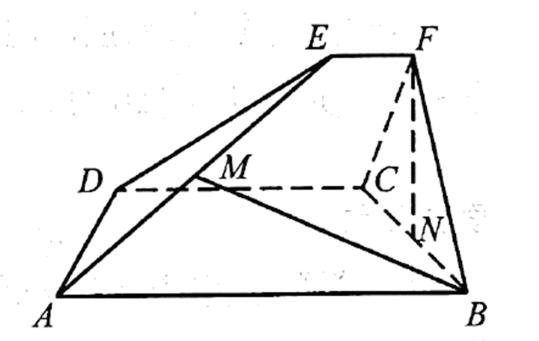
\includegraphics[width=.42\linewidth]{assets/asset-227-01.jpg}
\end{center}
\fillin[{$[12+2\sqrt{2}, 16]$}]
\begin{solution}
\textbf{答案：}$[12+2\sqrt{2}, 16]$

\textbf{分析：}根据正八边形的结构特征，分别以圆心为原点，$A_7A_3$ 所在直线为 $x$ 轴，$A_5A_1$ 所在直线为 $y$ 轴建立平面直角坐标系，即可求出各顶点的坐标，设 $P(x,y)$，再根据平面向量模的坐标计算公式即可得到 $\overrightarrow{PA_1}^2+\cdots+\overrightarrow{PA_8}^2 = 8(x^2+y^2)+8$，然后利用 $\cos 22.5^\circ \le |OP| \le 1$ 即可解出．

\textbf{详解：}建系如图，各顶点坐标：$A_1(0,1), A_2(\frac{\sqrt{2}}{2},\frac{\sqrt{2}}{2}), A_3(1,0), A_4(\frac{\sqrt{2}}{2},-\frac{\sqrt{2}}{2}), A_5(0,-1), A_6(-\frac{\sqrt{2}}{2},-\frac{\sqrt{2}}{2}), A_7(-1,0), A_8(-\frac{\sqrt{2}}{2},\frac{\sqrt{2}}{2})$．设 $P(x,y)$，则 $\sum PA_i^2 = 8(x^2+y^2)+8$．$|OP|$ 的最小值为 $\cos22.5^\circ = \frac{\sqrt{2+\sqrt{2}}}{2}$，最大值为1，所以 $x^2+y^2 \in [\frac{1+\cos45^\circ}{2},1] = [\frac{2+\sqrt{2}}{4},1]$，故取值范围为 $[12+2\sqrt{2},16]$.
\end{solution}
\end{question}

\begin{question}[points=14]
\textbf{来源：}2022 年 浙江卷，第 18 题\quad \textbf{专题：}三角形、三角函数\par
在 $\triangle ABC$ 中，角 $A,B,C$ 所对的边分别为 $a,b,c$．已知 $4a = \sqrt{5}c, \cos C = \frac{3}{5}$．

（1）求 $\sin A$ 的值；

（2）若 $b=11$，求 $\triangle ABC$ 的面积．
\begin{solution}
\textbf{答案：}（1）$\dfrac{\sqrt{5}}{5}$；（2）$22$

\textbf{分析：}（1）先由平方关系求出 $\sin C$，再根据正弦定理即可解出；（2）根据余弦定理以及 $4a=\sqrt{5}c$ 可解出 $a$，即可由三角形面积公式求出面积．

\textbf{详解：}（1）由 $\cos C = \frac{3}{5}$，$0<C<\pi$，得 $\sin C = \frac{4}{5}$．由 $4a=\sqrt{5}c$ 及正弦定理得 $4\sin A = \sqrt{5}\sin C$，所以 $\sin A = \frac{\sqrt{5}}{4}\cdot\frac{4}{5} = \frac{\sqrt{5}}{5}$．
（2）由 $4a=\sqrt{5}c$ 设 $c = \frac{4}{\sqrt{5}}a$，由余弦定理 $\cos C = \frac{a^2+b^2-c^2}{2ab} = \frac{a^2+121-\frac{16}{5}a^2}{2\cdot a\cdot11} = \frac{3}{5}$，解得 $a=5$（负值舍去），所以 $\triangle ABC$ 的面积 $S = \frac{1}{2}ab\sin C = \frac{1}{2}\times5\times11\times\frac{4}{5}=22$．
\end{solution}
\end{question}

\section*{2023 年}

\begin{question}[points=4]
\textbf{来源：}2023 年 北京卷，第 3 题\quad \textbf{专题：}向量\par
已知向量 $\vec{a}, \vec{b}$ 满足 $\vec{a} + \vec{b} = (2,3), \vec{a} - \vec{b} = (-2,1)$ ，则 $|\vec{a}|^2 - |\vec{b}|^2 =$ （ ）
\begin{choices}
  \item $-2$
  \item $-1$
  \item $0$
  \item $1$
\end{choices}
\begin{solution}
\textbf{答案：}B

\textbf{分析：}利用平面向量数量积的运算律，数量积的坐标表示求解作答.

\textbf{详解：}向量 $\vec{a}, \vec{b}$ 满足 $\vec{a} + \vec{b} = (2,3), \vec{a} - \vec{b} = (-2,1)$ ，所以 $|\vec{a}|^2 - |\vec{b}|^2 = (\vec{a}+\vec{b})\cdot(\vec{a}-\vec{b}) = 2\times(-2) + 3\times1 = -1$ .
\end{solution}
\end{question}

\begin{question}[points=4]
\textbf{来源：}2023 年 北京卷，第 7 题\quad \textbf{专题：}三角形、三角函数\par
在 $\triangle ABC$ 中， $(a+c)(\sin A - \sin C) = b(\sin A - \sin B)$ ，则 $\angle C =$ （ ）
\begin{choices}
  \item $\dfrac{\pi}{6}$
  \item $\dfrac{\pi}{3}$
  \item $\dfrac{2\pi}{3}$
  \item $\dfrac{5\pi}{6}$
\end{choices}
\begin{solution}
\textbf{答案：}B

\textbf{分析：}利用正弦定理的边角变换与余弦定理即可得解.

\textbf{详解：}因为 $(a+c)(\sin A - \sin C) = b(\sin A - \sin B)$，所以由正弦定理得 $(a+c)(a-c) = b(a-b)$，即 $a^2 - c^2 = ab - b^2$，则 $a^2 + b^2 - c^2 = ab$，故 $\cos C = \dfrac{a^2+b^2-c^2}{2ab} = \dfrac{ab}{2ab} = \dfrac{1}{2}$，又 $0 < C < \pi$，所以 $C = \dfrac{\pi}{3}$.
\end{solution}
\end{question}

\begin{question}[points=5]
\textbf{来源：}2023 年 北京卷，第 13 题\quad \textbf{专题：}三角函数\par
已知命题 $p$ : 若 $\alpha, \beta$ 为第一象限角，且 $\alpha > \beta$ ，则 $\tan \alpha > \tan \beta$ ．能说明 $p$ 为假命题的一组 $\alpha, \beta$ 的值为 $\alpha =$ ， $\beta =$ ．
\fillin[{$\dfrac{9\pi}{4}$ ; $\dfrac{\pi}{3}$}]
\begin{solution}
\textbf{答案：}$\dfrac{9\pi}{4}$ ; $\dfrac{\pi}{3}$

\textbf{分析：}根据正切函数单调性以及任意角的定义分析求解.

\textbf{详解：}因为 $f(x)=\tan x$ 在 $(0,\frac{\pi}{2})$ 上单调递增，若 $0<\alpha_0<\beta_0<\frac{\pi}{2}$，则 $\tan\alpha_0<\tan\beta_0$，取 $\alpha=2k_1\pi+\alpha_0, \beta=2k_2\pi+\beta_0, k_1,k_2\in\mathbb{Z}$，则 $\tan\alpha=\tan\alpha_0, \tan\beta=\tan\beta_0$，即 $\tan\alpha<\tan\beta$，令 $k_1>k_2$，则 $\alpha-\beta=2(k_1-k_2)\pi+(\alpha_0-\beta_0)>0$，即 $\alpha>\beta$。不妨取 $k_1=1,k_2=0,\alpha_0=\frac{\pi}{4},\beta_0=\frac{\pi}{3}$，即 $\alpha=\frac{9\pi}{4},\beta=\frac{\pi}{3}$ 满足题意。
\end{solution}
\end{question}

\begin{question}[points=13]
\textbf{来源：}2023 年 北京卷，第 17 题\quad \textbf{专题：}三角函数\par
设函数 $f(x) = \sin\omega x\cos\varphi + \cos\omega x\sin\varphi$ $\left(\omega>0, |\varphi|<\dfrac{\pi}{2}\right)$．

（1）若 $f(0) = -\dfrac{\sqrt{3}}{2}$ ，求 $\varphi$ 的值．

（2）已知 $f(x)$ 在区间 $\left[-\dfrac{\pi}{3}, \dfrac{2\pi}{3}\right]$ 上单调递增， $f\left(\dfrac{2\pi}{3}\right)=1$ ，再从条件①、条件②、条件③这三个条件中选择一个作为已知，使函数 $f(x)$ 存在，求 $\omega, \varphi$ 的值．

条件①：$f\left(\dfrac{\pi}{3}\right)=\sqrt{2}$；

条件②：$f\left(-\dfrac{\pi}{3}\right)=-1$；

条件③：$f(x)$ 在区间 $\left[-\dfrac{\pi}{2}, -\dfrac{\pi}{3}\right]$ 上单调递减．

注：如果选择的条件不符合要求，第（2）问得0分；如果选择多个符合要求的条件分别解答，按第一个解答计分．
\begin{solution}
\textbf{答案：}（1）$\varphi=-\dfrac{\pi}{3}$ （2）条件①不能使函数$f(x)$存在；条件②或条件③可解得$\omega=1$，$\varphi=-\dfrac{\pi}{6}$

\textbf{分析：}（1）把$x=0$代入$f(x)$的解析式求出$\sin\varphi$，再由$|\varphi|<\frac{\pi}{2}$即可求出$\varphi$的值；（2）若选条件①不合题意；若选条件②，先把$f(x)$的解析式化简，根据$f(x)$在$[-\frac{\pi}{3},\frac{2\pi}{3}]$上的单调性及函数的最值可求出$T$，从而求出$\omega$的值；把$\omega$的值代入$f(x)$的解析式，由$f(-\frac{\pi}{3})=-1$和$|\varphi|<\frac{\pi}{2}$即可求出$\varphi$的值；若选条件③：由$f(x)$的单调性可知$f(x)$在$x=-\frac{\pi}{3}$处取得最小值$-1$，则与条件②所给的条件一样，解法与条件②相同.

\textbf{详解：}（1）因为 $f(x)=\sin\omega x\cos\varphi+\cos\omega x\sin\varphi$, $\omega>0$, $|\varphi|<\frac{\pi}{2}$，所以 $f(0)=\sin0\cos\varphi+\cos0\sin\varphi=\sin\varphi=-\frac{\sqrt{3}}{2}$，因为 $|\varphi|<\frac{\pi}{2}$，所以 $\varphi=-\frac{\pi}{3}$。
（2）$f(x)=\sin(\omega x+\varphi)$，$\omega>0$, $|\varphi|<\frac{\pi}{2}$，所以 $f(x)$ 的最大值为1，最小值为-1。若选条件①：因为 $f(x)$ 的最大值为1，最小值为-1，所以 $f(\frac{\pi}{3})=\sqrt{2}$ 无解，故条件①不能使函数 $f(x)$ 存在；若选条件②：因为 $f(x)$ 在 $[-\frac{\pi}{3},\frac{2\pi}{3}]$ 上单调递增，且 $f(\frac{2\pi}{3})=1$，$f(-\frac{\pi}{3})=-1$，所以 $\frac{T}{2}=\frac{2\pi}{3}-(-\frac{\pi}{3})=\pi$，所以 $T=2\pi$，$\omega=\frac{2\pi}{T}=1$，所以 $f(x)=\sin(x+\varphi)$，又因为 $f(-\frac{\pi}{3})=-1$，所以 $\sin(-\frac{\pi}{3}+\varphi)=-1$，所以 $-\frac{\pi}{3}+\varphi=-\frac{\pi}{2}+2k\pi$，$k\in\mathbb{Z}$，所以 $\varphi=-\frac{\pi}{6}+2k\pi$，因为 $|\varphi|<\frac{\pi}{2}$，所以 $\varphi=-\frac{\pi}{6}$。所以 $\omega=1$，$\varphi=-\frac{\pi}{6}$；若选条件③：因为 $f(x)$ 在 $[-\frac{\pi}{3},\frac{2\pi}{3}]$ 上单调递增，在 $[-\frac{\pi}{2},-\frac{\pi}{3}]$ 上单调递减，所以 $f(x)$ 在 $x=-\frac{\pi}{3}$ 处取得最小值 $-1$，即 $f(-\frac{\pi}{3})=-1$。以下与条件②相同。
\end{solution}
\end{question}

\begin{question}[points=5]
\textbf{来源：}2023 年 全国甲卷-理科，第 4 题\quad \textbf{专题：}向量、三角函数\par
已知向量 $\vec{a}$，$\vec{b}$，$\vec{c}$ 满足 $|\vec{a}| = |\vec{b}| = 1$，$|\vec{c}| = \sqrt{2}$，且 $\vec{a} + \vec{b} + \vec{c} = 0$，则 $\cos\langle \vec{a} - \vec{c}, \vec{b} - \vec{c} \rangle = $ （               ）
\begin{choices}
  \item $-\frac{4}{5}$
  \item $-\frac{2}{5}$
  \item $\frac{2}{5}$
  \item $\frac{4}{5}$
\end{choices}
\begin{solution}
\textbf{答案：}D

\textbf{分析：}作出图形，根据几何意义求解．

\textbf{详解：}因为 $\vec{a} + \vec{b} + \vec{c} = \vec{0}$，所以 $\vec{a} + \vec{b} = -\vec{c}$，即 $|\vec{a}|^2 + |\vec{b}|^2 + 2\vec{a} \cdot \vec{b} = |\vec{c}|^2$，即 $1 + 1 + 2\vec{a} \cdot \vec{b} = 2$，所以 $\vec{a} \cdot \vec{b} = 0$．如图，设 $\overrightarrow{OA} = \vec{a}$，$\overrightarrow{OB} = \vec{b}$，$\overrightarrow{OC} = \vec{c}$，由题知 $OA = OB = 1$，$OC = \sqrt{2}$，$\triangle OAB$ 是等腰直角三角形，$AB$ 边上的高 $OD = \frac{\sqrt{2}}{2}$，$AD = \frac{\sqrt{2}}{2}$，所以 $CD = CO + OD = \sqrt{2} + \frac{\sqrt{2}}{2} = \frac{3\sqrt{2}}{2}$，$\tan \angle ACD = \frac{AD}{CD} = \frac{1}{3}$，$\cos \angle ACD = \frac{3}{\sqrt{10}}$，$\cos\langle \vec{a} - \vec{c}, \vec{b} - \vec{c} \rangle = \cos \angle ACB = \cos 2\angle ACD = 2\cos^2 \angle ACD - 1 = 2 \times \frac{9}{10} - 1 = \frac{4}{5}$．
\end{solution}
\end{question}

\begin{question}[points=5]
\textbf{来源：}2023 年 全国甲卷-理科，第 7 题\quad \textbf{专题：}三角函数\par
设甲：$\sin^2 \alpha + \sin^2 \beta = 1$，乙：$\sin \alpha + \cos \beta = 0$，则（           ）
\begin{choices}
  \item 甲是乙的充分条件但不是必要条件
  \item 甲是乙的必要条件但不是充分条件
  \item 甲是乙的充要条件
  \item 甲既不是乙的充分条件也不是乙的必要条件
\end{choices}
\begin{solution}
\textbf{答案：}B

\textbf{分析：}根据充分条件、必要条件的概念及同角三角函数的基本关系得解．

\textbf{详解：}当 $\sin^2 \alpha + \sin^2 \beta = 1$ 时，例如 $\alpha = \frac{\pi}{2}, \beta = 0$，但 $\sin \alpha + \cos \beta \neq 0$，即 $\sin^2 \alpha + \sin^2 \beta = 1$ 推不出 $\sin \alpha + \cos \beta = 0$；当 $\sin \alpha + \cos \beta = 0$ 时，$\sin^2 \alpha + \sin^2 \beta = (-\cos \beta)^2 + \sin^2 \beta = 1$，即 $\sin \alpha + \cos \beta = 0$ 能推出 $\sin^2 \alpha + \sin^2 \beta = 1$．综上可知，甲是乙的必要不充分条件．
\end{solution}
\end{question}

\begin{question}[points=5]
\textbf{来源：}2023 年 全国甲卷-理科，第 10 题\quad \textbf{专题：}三角函数\par
函数 $y = f(x)$ 的图象由函数 $y = \cos\left(2x + \frac{\pi}{6}\right)$ 的图象向左平移 $\frac{\pi}{6}$ 个单位长度得到，则 $y = f(x)$ 的图象与直线 $y = \frac{1}{2}x - \frac{1}{2}$ 的交点个数为（                  ）
\begin{choices}
  \item $1$
  \item $2$
  \item $3$
  \item $4$
\end{choices}
\begin{solution}
\textbf{答案：}C

\textbf{分析：}先利用三角函数平移的性质求得 $f(x) = -\sin 2x$，再作出 $f(x)$ 与 $y = \frac{1}{2}x - \frac{1}{2}$ 的部分大致图像，考虑特殊点处 $f(x)$ 与 $y = \frac{1}{2}x - \frac{1}{2}$ 的大小关系，从而精确图像，由此得解．

\textbf{详解：}因为 $y = \cos\left(2x + \frac{\pi}{6}\right)$ 向左平移 $\frac{\pi}{6}$ 个单位所得函数为 $y = \cos\left[2\left(x + \frac{\pi}{6}\right) + \frac{\pi}{6}\right] = \cos\left(2x + \frac{\pi}{2}\right) = -\sin 2x$，所以 $f(x) = -\sin 2x$，而 $y = \frac{1}{2}x - \frac{1}{2}$ 显然过 $(0, -\frac{1}{2})$ 与 $(1,0)$ 两点，作出 $f(x)$ 与 $y = \frac{1}{2}x - \frac{1}{2}$ 的部分大致图像如下，考虑 $2x = -\frac{3\pi}{2}, 2x = \frac{3\pi}{2}, 2x = \frac{7\pi}{2}$，即 $x = -\frac{3\pi}{4}, x = \frac{3\pi}{4}, x = \frac{7\pi}{4}$ 处 $f(x)$ 与 $y = \frac{1}{2}x - \frac{1}{2}$ 的大小关系，当 $x = -\frac{3\pi}{4}$ 时，$f(-\frac{3\pi}{4}) = -\sin\left(-\frac{3\pi}{2}\right) = -1$，$y = \frac{1}{2}\times\left(-\frac{3\pi}{4}\right) - \frac{1}{2} = -\frac{3\pi+4}{8} < -1$；当 $x = \frac{3\pi}{4}$ 时，$f(\frac{3\pi}{4}) = -\sin\frac{3\pi}{2} = 1$，$y = \frac{1}{2}\times\frac{3\pi}{4} - \frac{1}{2} = \frac{3\pi-4}{8} < 1$；当 $x = \frac{7\pi}{4}$ 时，$f(\frac{7\pi}{4}) = -\sin\frac{7\pi}{2} = 1$，$y = \frac{1}{2}\times\frac{7\pi}{4} - \frac{1}{2} = \frac{7\pi-4}{8} > 1$；所以由图可知，$f(x)$ 与 $y = \frac{1}{2}x - \frac{1}{2}$ 的交点个数为 3．
\end{solution}
\end{question}

\begin{question}[points=5]
\textbf{来源：}2023 年 全国甲卷-理科，第 12 题\quad \textbf{专题：}三角函数\par
设 $O$ 为坐标原点，$F_1$，$F_2$ 为椭圆 $C: \frac{x^2}{9} + \frac{y^2}{6} = 1$ 的两个焦点，点 $P$ 在 $C$ 上，$\cos\angle F_1PF_2 = \frac{3}{5}$，则 $|OP| = $（         ）
\begin{choices}
  \item $\frac{\sqrt{13}}{5}$
  \item $\frac{\sqrt{30}}{2}$
  \item $\frac{\sqrt{14}}{5}$
  \item $\frac{\sqrt{35}}{2}$
\end{choices}
\begin{solution}
\textbf{答案：}B

\textbf{分析：}方法一：根据焦点三角形面积公式求出 $\triangle PF_1F_2$ 的面积，即可得到点 $P$ 的坐标，从而得出 $OP$ 的值；方法二：利用椭圆的定义以及余弦定理求出 $|PF_1||PF_2|$，$|PF_1|^2+|PF_2|^2$，再结合中线的向量公式以及数量积即可求出；方法三：利用椭圆的定义以及余弦定理求出 $|PF_1|^2+|PF_2|^2$，即可根据中线定理求出．

\textbf{详解：}方法一：设 $\angle F_1PF_2 = 2\theta$，$0<\theta<\frac{\pi}{2}$，所以 $S_{\triangle PF_1F_2} = b^2\tan\frac{\angle F_1PF_2}{2} = b^2\tan\theta$，由 $\cos\angle F_1PF_2 = \cos2\theta = \frac{\cos^2\theta-\sin^2\theta}{\cos^2\theta+\sin^2\theta} = \frac{1-\tan^2\theta}{1+\tan^2\theta} = \frac{3}{5}$，解得：$\tan\theta = \frac{1}{2}$，由椭圆方程可知，$a^2=9$，$b^2=6$，$c^2=a^2-b^2=3$，所以 $S_{\triangle PF_1F_2} = \frac{1}{2}\times F_1F_2\times|y_p| = \frac{1}{2}\times2\sqrt{3}\times|y_p| = 6\times\frac{1}{2}$，解得：$y_p^2=3$，则 $x_p^2 = 9\times\left(1-\frac{3}{6}\right) = \frac{9}{2}$，因此 $|OP| = \sqrt{x_p^2+y_p^2} = \sqrt{3+\frac{9}{2}} = \frac{\sqrt{30}}{2}$．故选：B．
方法二：因为 $|PF_1|+|PF_2|=2a=6$ ①，$|PF_1|^2+|PF_2|^2-2|PF_1||PF_2|\cos\angle F_1PF_2 = |F_1F_2|^2$，即 $|PF_1|^2+|PF_2|^2 - \frac{6}{5}|PF_1||PF_2| = 12$ ②，联立①②，解得：$|PF_1||PF_2| = \frac{15}{2}$，$|PF_1|^2+|PF_2|^2 = 21$，而 $\overrightarrow{PO} = \frac{1}{2}(\overrightarrow{PF_1}+\overrightarrow{PF_2})$，所以 $|\overrightarrow{OP}| = |\overrightarrow{PO}| = \frac{1}{2}\sqrt{|\overrightarrow{PF_1}|^2+|\overrightarrow{PF_2}|^2+2\overrightarrow{PF_1}\cdot\overrightarrow{PF_2}} = \frac{1}{2}\sqrt{21+2\times\frac{3}{5}\times\frac{15}{2}} = \frac{\sqrt{30}}{2}$．故选：B．
方法三：因为 $|PF_1|+|PF_2|=2a=6$ ①，$|PF_1|^2+|PF_2|^2-2|PF_1||PF_2|\cos\angle F_1PF_2 = |F_1F_2|^2$，即 $|PF_1|^2+|PF_2|^2 - \frac{6}{5}|PF_1||PF_2| = 12$ ②，联立①②，解得：$|PF_1|^2+|PF_2|^2 = 21$，由中线定理可知，$2(|OP|^2+|OF_1|^2) = |PF_1|^2+|PF_2|^2 = 42$，易知 $|F_1F_2| = 2\sqrt{3}$，解得：$|OP| = \frac{\sqrt{30}}{2}$．故选：B．
\end{solution}
\end{question}

\begin{question}[points=5]
\textbf{来源：}2023 年 全国甲卷-理科，第 13 题\quad \textbf{专题：}三角函数\par
若 $f(x) = (x-1)^2 + ax + \sin\left(x + \frac{\pi}{2}\right)$ 为偶函数，则 $a = $．
\fillin[{$2$}]
\begin{solution}
\textbf{答案：}$2$

\textbf{分析：}利用偶函数的性质得到 $f\left(-\frac{\pi}{2}\right) = f\left(\frac{\pi}{2}\right)$，从而求得 $a=2$，再检验即可得解．

\textbf{详解：}因为 $y = f(x) = (x-1)^2 + ax + \sin\left(x+\frac{\pi}{2}\right) = (x-1)^2 + ax + \cos x$ 为偶函数，定义域为 $R$，所以 $f\left(-\frac{\pi}{2}\right) = f\left(\frac{\pi}{2}\right)$，即 $\left(-\frac{\pi}{2}-1\right)^2 - a\frac{\pi}{2} + \cos\left(-\frac{\pi}{2}\right) = \left(\frac{\pi}{2}-1\right)^2 + a\frac{\pi}{2} + \cos\frac{\pi}{2}$，则 $\pi a = \left(\frac{\pi}{2}+1\right)^2 - \left(\frac{\pi}{2}-1\right)^2 = 2\pi$，故 $a=2$，此时 $f(x) = (x-1)^2 + 2x + \cos x = x^2 + 1 + \cos x$，所以 $f(-x) = (-x)^2 + 1 + \cos(-x) = x^2+1+\cos x = f(x)$，又定义域为 $R$，故 $f(x)$ 为偶函数，所以 $a=2$．
\end{solution}
\end{question}

\begin{question}[points=5]
\textbf{来源：}2023 年 全国甲卷-理科，第 16 题\quad \textbf{专题：}三角形、三角函数\par
在 $\triangle ABC$ 中，$\angle BAC = 60^\circ$，$AB = 2$，$BC = \sqrt{6}$，$\angle BAC$ 的角平分线交 $BC$ 于 $D$，则 $AD = $．
\fillin[{$2$}]
\begin{solution}
\textbf{答案：}$2$

\textbf{分析：}方法一：利用余弦定理求出 $AC$，再根据等面积法求出 $AD$；方法二：利用余弦定理求出 $AC$，再根据正弦定理求出 $B$，$C$，即可根据三角形的特征求出．

\textbf{详解：}方法一：记 $AB=c$，$AC=b$，$BC=a$，由余弦定理可得，$2^2+b^2-2\times2\times b\times\cos60^\circ = 6$，因为 $b>0$，解得：$b=1+\sqrt{3}$，由 $S_{\triangle ABC} = S_{\triangle ABD} + S_{\triangle ACD}$ 可得，$\frac{1}{2}\times2\times b\times\sin60^\circ = \frac{1}{2}\times2\times AD\times\sin30^\circ + \frac{1}{2}\times AD\times b\times\sin30^\circ$，解得：$AD = \frac{\sqrt{3}b}{1+\frac{b}{2}} = \frac{\sqrt{3}(1+\sqrt{3})}{\frac{3+\sqrt{3}}{2}} = 2$．故答案为：2．
方法二：由余弦定理可得，$2^2+b^2-2\times2\times b\times\cos60^\circ = 6$，因为 $b>0$，解得：$b=1+\sqrt{3}$，由正弦定理可得，$\frac{\sqrt{6}}{\sin60^\circ} = \frac{b}{\sin B} = \frac{2}{\sin C}$，解得：$\sin B = \frac{\sqrt{6}+\sqrt{2}}{4}$，$\sin C = \frac{\sqrt{2}}{2}$，因为 $1+\sqrt{3} > \sqrt{6} > 2$，所以 $C=45^\circ$，$B=180^\circ-60^\circ-45^\circ=75^\circ$，又 $\angle BAD = 30^\circ$，所以 $\angle ADB = 75^\circ$，即 $AD = AB = 2$．故答案为：2．
\end{solution}
\end{question}

\begin{question}[points=12]
\textbf{来源：}2023 年 全国甲卷-理科，第 20 题\quad \textbf{专题：}向量\par
已知直线 $x-2y+1=0$ 与抛物线 $C: y^2 = 2px (p>0)$ 交于 $A$，$B$ 两点，且 $|AB| = 4\sqrt{15}$．

（1）求 $p$；

（2）设 $F$ 为 $C$ 的焦点，$M$，$N$ 为 $C$ 上两点，$\overrightarrow{FM} \cdot \overrightarrow{FN} = 0$，求 $\triangle MFN$ 面积的最小值．
\begin{solution}
\textbf{答案：}（1）$p=2$；（2）$12-8\sqrt{2}$

\textbf{分析：}（1）利用直线与抛物线的位置关系，联立直线和抛物线方程求出弦长即可得出 $p$；（2）设直线 $MN: x = my + n$，$M(x_1,y_1)$，$N(x_2,y_2)$，利用 $\overrightarrow{FM}\cdot\overrightarrow{FN}=0$，找到 $m,n$ 的关系，以及 $\triangle MFN$ 的面积表达式，再结合函数的性质即可求出其最小值．

\textbf{详解：}（1）设 $A(x_A,y_A)$，$B(x_B,y_B)$，由 $\begin{cases} x-2y+1=0 \\ y^2=2px \end{cases}$ 可得，$y^2-4py+2p=0$，所以 $y_A+y_B=4p$，$y_Ay_B=2p$，所以 $|AB| = \sqrt{(x_A-x_B)^2+(y_A-y_B)^2} = \sqrt{5}|y_A-y_B| = \sqrt{5}\times\sqrt{(y_A+y_B)^2-4y_Ay_B} = 4\sqrt{15}$，即 $2p^2-p-6=0$，因为 $p>0$，解得：$p=2$．
（2）因为 $F(1,0)$，显然直线 $MN$ 的斜率不可能为零，设直线 $MN: x = my + n$，$M(x_1,y_1)$，$N(x_2,y_2)$，由 $\begin{cases} y^2=4x \\ x=my+n \end{cases}$ 可得，$y^2-4my-4n=0$，所以 $y_1+y_2=4m$，$y_1y_2=-4n$，$\Delta = 16m^2+16n>0 \Rightarrow m^2+n>0$，因为 $\overrightarrow{FM}\cdot\overrightarrow{FN}=0$，所以 $(x_1-1)(x_2-1)+y_1y_2=0$，即 $(my_1+n-1)(my_2+n-1)+y_1y_2=0$，亦即 $(m^2+1)y_1y_2 + m(n-1)(y_1+y_2) + (n-1)^2=0$，将 $y_1+y_2=4m$，$y_1y_2=-4n$ 代入得，$4m^2 = n^2-6n+1$，$4(m^2+n) = (n-1)^2>0$，所以 $n\neq1$，且 $n^2-6n+1\ge0$，解得 $n\ge 3+2\sqrt{2}$ 或 $n\le 3-2\sqrt{2}$．设点 $F$ 到直线 $MN$ 的距离为 $d$，所以 $d = \frac{|n-1|}{\sqrt{1+m^2}}$，$|MN| = \sqrt{(x_1-x_2)^2+(y_1-y_2)^2} = \sqrt{1+m^2}|y_1-y_2| = \sqrt{1+m^2}\sqrt{16m^2+16n} = 2\sqrt{1+m^2}\sqrt{4(n^2-6n+1)+16n} = 2\sqrt{1+m^2}|n-1|$，所以 $\triangle MFN$ 的面积 $S = \frac{1}{2}\times|MN|\times d = \frac{1}{2}\times\frac{|n-1|}{\sqrt{1+m^2}}\times2\sqrt{1+m^2}|n-1| = (n-1)^2$，而 $n\ge 3+2\sqrt{2}$ 或 $n\le 3-2\sqrt{2}$，所以，当 $n=3-2\sqrt{2}$ 时，$\triangle MFN$ 的面积 $S_{\min} = (2-2\sqrt{2})^2 = 12-8\sqrt{2}$．
\end{solution}
\end{question}

\begin{question}[points=12]
\textbf{来源：}2023 年 全国甲卷-理科，第 21 题\quad \textbf{专题：}三角函数\par
已知函数 $f(x) = ax - \frac{\sin x}{\cos^3 x}$，$x \in \left(0, \frac{\pi}{2}\right)$．

（1）当 $a=8$ 时，讨论 $f(x)$ 的单调性；

（2）若 $f(x) < \sin 2x$ 恒成立，求 $a$ 的取值范围．
\begin{solution}
\textbf{答案：}（1）$f(x)$ 在 $(0,\frac{\pi}{4})$ 上单调递增，在 $(\frac{\pi}{4},\frac{\pi}{2})$ 上单调递减；（2）$(-\infty,3]$

\textbf{分析：}（1）求导，然后令 $t=\cos^2 x$，讨论导数的符号即可；（2）构造 $g(x)=f(x)-\sin 2x$，计算 $g'(x)$ 的最大值，然后与 0 比较大小，得出 $a$ 的分界点，再对 $a$ 讨论即可．

\textbf{详解：}（1）$f'(x) = a - \frac{\cos x \cos^3 x + 3\sin x \cos^2 x \sin x}{\cos^6 x} = a - \frac{\cos^2 x + 3\sin^2 x}{\cos^4 x} = a - \frac{3-2\cos^2 x}{\cos^4 x}$，令 $\cos^2 x = t$，则 $t\in(0,1)$，则 $f'(x) = g(t) = a - \frac{3-2t}{t^2} = \frac{at^2+2t-3}{t^2}$，当 $a=8$ 时，$f'(x) = g(t) = \frac{8t^2+2t-3}{t^2} = \frac{(2t-1)(4t+3)}{t^2}$，当 $t\in(0,\frac{1}{2})$ 时，$f'(x)<0$；当 $t\in(\frac{1}{2},1)$ 时，$f'(x)>0$．所以 $f(x)$ 在 $(0,\frac{\pi}{4})$ 上单调递增，在 $(\frac{\pi}{4},\frac{\pi}{2})$ 上单调递减．
（2）设 $g(x)=f(x)-\sin 2x$，$g'(x)=f'(x)-2\cos 2x = g(t) - 2(2\cos^2 x -1) = \frac{at^2+2t-3}{t^2} - 2(2t-1) = a+2 - 4t + \frac{2}{t} - \frac{3}{t^2}$，设 $\varphi(t)=a+2-4t+\frac{2}{t}-\frac{3}{t^2}$，$\varphi'(t)=-4-\frac{2}{t^2}+\frac{6}{t^3} = \frac{-4t^3-2t+6}{t^3} = -\frac{2(t-1)(2t^2+2t+3)}{t^3}>0$，所以 $\varphi(t)<\varphi(1)=a-3$．①若 $a\in(-\infty,3]$，$g'(x)=\varphi(t)<a-3\le0$，即 $g(x)$ 在 $(0,\frac{\pi}{2})$ 上单调递减，所以 $g(x)<g(0)=0$，所以当 $a\in(-\infty,3]$ 时，$f(x)<\sin 2x$，符合题意．②若 $a\in(3,+\infty)$，当 $t\to0$ 时，$\frac{2}{t}-\frac{3}{t^2} = -3\left(\frac{1}{t}-\frac{1}{3}\right)^2+\frac{1}{3} \to -\infty$，所以 $\varphi(t)\to -\infty$，$\varphi(1)=a-3>0$，所以 $\exists t_0\in(0,1)$，使得 $\varphi(t_0)=0$，即 $\exists x_0\in(0,\frac{\pi}{2})$，使得 $g'(x_0)=0$．当 $t\in(t_0,1)$ 时，$\varphi(t)>0$，即当 $x\in(0,x_0)$ 时，$g'(x)>0$，$g(x)$ 单调递增，所以当 $x\in(0,x_0)$ 时，$g(x)>g(0)=0$，不合题意．综上，$a$ 的取值范围为 $(-\infty,3]$．
\end{solution}
\end{question}

\begin{question}[points=5]
\textbf{来源：}2023 年 全国甲卷-文科，第 3 题\quad \textbf{专题：}三角函数、向量\par
已知向量 $\vec{a} = (3,1), \vec{b} = (2,2)$，则 $\cos\langle \vec{a}+\vec{b}, \vec{a}-\vec{b} \rangle =$（    ）
\begin{choices}
  \item $\frac{1}{17}$
  \item $\frac{\sqrt{17}}{17}$
  \item $\frac{\sqrt{5}}{5}$
  \item $\frac{2\sqrt{5}}{5}$
\end{choices}
\begin{solution}
\textbf{答案：}B

\textbf{分析：}利用平面向量模与数量积的坐标表示分别求得 $|\vec{a}+\vec{b}|, |\vec{a}-\vec{b}|, (\vec{a}+\vec{b})\cdot(\vec{a}-\vec{b})$，从而利用平面向量余弦的运算公式即可得解.

\textbf{详解：}因为 $\vec{a} = (3,1), \vec{b} = (2,2)$，所以 $\vec{a}+\vec{b} = (5,3), \vec{a}-\vec{b} = (1,-1)$，则 $|\vec{a}+\vec{b}| = \sqrt{5^2+3^2} = \sqrt{34}, |\vec{a}-\vec{b}| = \sqrt{1+1} = \sqrt{2}, (\vec{a}+\vec{b})\cdot(\vec{a}-\vec{b}) = 5\times1+3\times(-1)=2$，所以 $\cos\langle \vec{a}+\vec{b}, \vec{a}-\vec{b} \rangle = \frac{2}{\sqrt{34}\times\sqrt{2}} = \frac{\sqrt{17}}{17}$，故选B.
\end{solution}
\end{question}

\begin{question}[points=5]
\textbf{来源：}2023 年 全国甲卷-文科，第 7 题\quad \textbf{专题：}向量\par
设 $F_1, F_2$ 为椭圆 $C: \frac{x^2}{5}+y^2=1$ 的两个焦点，点 $P$ 在 $C$ 上，若 $\overrightarrow{PF_1} \cdot \overrightarrow{PF_2}=0$，则 $PF_1 \cdot PF_2 =$（    ）
\begin{choices}
  \item $1$
  \item $2$
  \item $4$
  \item $5$
\end{choices}
\begin{solution}
\textbf{答案：}B

\textbf{分析：}方法一：根据焦点三角形面积公式求出 $\triangle PF_1F_2$ 的面积，即可解出；方法二：根据椭圆的定义以及勾股定理即可解出．

\textbf{详解：}方法一：因为 $\overrightarrow{PF_1} \cdot \overrightarrow{PF_2}=0$，所以 $\angle F_1PF_2=90^\circ$，从而 $S_{\triangle PF_1F_2} = b^2\tan45^\circ = 1 = \frac{1}{2} \cdot PF_1 \cdot PF_2$，所以 $PF_1 \cdot PF_2 = 2$．故选B.
方法二：因为 $\overrightarrow{PF_1} \cdot \overrightarrow{PF_2}=0$，所以 $\angle F_1PF_2=90^\circ$，由椭圆方程可知，$c^2=5-1=4 \Rightarrow c=2$，所以 $PF_1^2+PF_2^2 = F_1F_2^2 = 4^2=16$，又 $PF_1+PF_2=2a=2\sqrt{5}$，平方得：$PF_1^2+PF_2^2+2PF_1PF_2=16+2PF_1PF_2=20$，所以 $PF_1 \cdot PF_2=2$．故选B.
\end{solution}
\end{question}

\begin{question}[points=5]
\textbf{来源：}2023 年 全国甲卷-文科，第 12 题\quad \textbf{专题：}三角函数\par
函数 $y=f(x)$ 的图象由 $y=\cos\left(2x+\frac{\pi}{6}\right)$ 的图象向左平移 $\frac{\pi}{6}$ 个单位长度得到，则 $y=f(x)$ 的图象与直线 $y=\frac{1}{2}x-\frac{1}{2}$ 的交点个数为（    ）
\begin{choices}
  \item $1$
  \item $2$
  \item $3$
  \item $4$
\end{choices}
\begin{solution}
\textbf{答案：}C

\textbf{分析：}先利用三角函数平移的性质求得 $f(x)=-\sin2x$，再作出 $f(x)$ 与 $y=\frac{1}{2}x-\frac{1}{2}$ 的部分大致图像，考虑特殊点处 $f(x)$ 与 $y=\frac{1}{2}x-\frac{1}{2}$ 的大小关系，从而精确图像，由此得解.

\textbf{详解：}因为 $y=\cos\left(2x+\frac{\pi}{6}\right)$ 向左平移 $\frac{\pi}{6}$ 个单位所得函数为 $y=\cos\left[2(x+\frac{\pi}{6})+\frac{\pi}{6}\right]=\cos\left(2x+\frac{\pi}{2}\right)=-\sin2x$，所以 $f(x)=-\sin2x$，而 $y=\frac{1}{2}x-\frac{1}{2}$ 显然过 $(0,-\frac{1}{2})$ 与 $(1,0)$ 两点，作出 $f(x)$ 与 $y=\frac{1}{2}x-\frac{1}{2}$ 的部分大致图像，考虑 $2x=-\frac{3\pi}{2},2x=\frac{3\pi}{2},2x=\frac{7\pi}{2}$，即 $x=-\frac{3\pi}{4},x=\frac{3\pi}{4},x=\frac{7\pi}{4}$ 处 $f(x)$ 与 $y=\frac{1}{2}x-\frac{1}{2}$ 的大小关系，当 $x=-\frac{3\pi}{4}$ 时，$f(-\frac{3\pi}{4})=-\sin(-\frac{3\pi}{2})=-1$，$y=\frac{1}{2}\times(-\frac{3\pi}{4})-\frac{1}{2}=-\frac{3\pi+4}{8}<-1$；当 $x=\frac{3\pi}{4}$ 时，$f(\frac{3\pi}{4})=-\sin\frac{3\pi}{2}=1$，$y=\frac{1}{2}\times\frac{3\pi}{4}-\frac{1}{2}=\frac{3\pi-4}{8}<1$；当 $x=\frac{7\pi}{4}$ 时，$f(\frac{7\pi}{4})=-\sin\frac{7\pi}{2}=1$，$y=\frac{1}{2}\times\frac{7\pi}{4}-\frac{1}{2}=\frac{7\pi-4}{8}>1$；所以由图可知，$f(x)$ 与 $y=\frac{1}{2}x-\frac{1}{2}$ 的交点个数为3，故选C.
\end{solution}
\end{question}

\begin{question}[points=5]
\textbf{来源：}2023 年 全国甲卷-文科，第 14 题\quad \textbf{专题：}三角函数\par
若 $f(x)=(x-1)^2+ax+\sin\left(x+\frac{\pi}{2}\right)$ 为偶函数，则 $a=$ ．
\fillin[{$2$}]
\begin{solution}
\textbf{答案：}$2$

\textbf{分析：}根据常见函数的奇偶性直接求解即可.

\textbf{详解：}因为 $f(x)=(x-1)^2+ax+\sin\left(x+\frac{\pi}{2}\right) = (x-1)^2+ax+\cos x = x^2+(a-2)x+1+\cos x$，且函数为偶函数，所以 $a-2=0$，解得 $a=2$．
\end{solution}
\end{question}

\begin{question}
\textbf{来源：}2023 年 全国甲卷-文科，第 17 题\quad \textbf{专题：}三角函数\par
记 $\triangle ABC$ 的内角 $A,B,C$ 的对边分别为 $a,b,c$，已知 $\frac{b^2+c^2-a^2}{\cos A}=2$．

（1）求 $bc$；

（2）若 $\frac{a\cos B-b\cos A}{a\cos B+b\cos A}-\frac{b}{c}=1$，求 $\triangle ABC$ 面积．
\begin{solution}
\textbf{答案：}（1）$bc=1$；（2）$\frac{\sqrt{3}}{4}$

\textbf{分析：}（1）根据余弦定理即可解出；（2）由（1）可知，只需求出 $\sin A$ 即可得到三角形面积，对等式恒等变换，即可解出．

\textbf{详解：}（1）因为 $a^2=b^2+c^2-2bc\cos A$，所以 $\frac{b^2+c^2-a^2}{\cos A}=\frac{2bc\cos A}{\cos A}=2bc=2$，解得 $bc=1$．
（2）由正弦定理可得 $\frac{a\cos B-b\cos A}{a\cos B+b\cos A}-\frac{b}{c}=\frac{\sin A\cos B-\sin B\cos A}{\sin A\cos B+\sin B\cos A}-\frac{\sin B}{\sin C}=\frac{\sin(A-B)}{\sin(A+B)}-\frac{\sin B}{\sin(A+B)}=\frac{\sin(A-B)-\sin B}{\sin(A+B)}=1$，变形可得 $\sin(A-B)-\sin(A+B)=\sin B$，即 $-2\cos A\sin B=\sin B$，而 $0<\sin B\le1$，所以 $\cos A=-\frac{1}{2}$，又 $0<A<\pi$，所以 $\sin A=\frac{\sqrt{3}}{2}$，故 $\triangle ABC$ 的面积为 $S_{\triangle ABC}=\frac{1}{2}bc\sin A=\frac{1}{2}\times1\times\frac{\sqrt{3}}{2}=\frac{\sqrt{3}}{4}$．
\end{solution}
\end{question}

\begin{question}
\textbf{来源：}2023 年 全国甲卷-文科，第 20 题\quad \textbf{专题：}三角函数\par
已知函数 $f(x)=ax-\frac{\sin x}{\cos^2 x}, x\in(0,\frac{\pi}{2})$．

（1）当 $a=1$ 时，讨论 $f(x)$ 的单调性；

（2）若 $f(x)+\sin x<0$，求 $a$ 的取值范围．
\begin{solution}
\textbf{答案：}（1）$f(x)$ 在 $(0,\frac{\pi}{2})$ 上单调递减；（2）$a\le0$

\textbf{分析：}（1）代入 $a=1$ 后，再对 $f(x)$ 求导，同时利用三角函数的平方关系化简 $f'(x)$，再利用换元法判断得其分子与分母的正负情况，从而得解；（2）法一：构造函数 $g(x)=f(x)+\sin x$，从而得到 $g(x)<0$，注意到 $g(0)=0$，从而得到 $g'(0)\le0$，进而得到 $a\le0$，再分类讨论 $a=0$ 与 $a<0$ 两种情况即可得解；法二：先化简并判断得 $\sin x-\frac{\sin x}{\cos^2 x}<0$ 恒成立，再分类讨论 $a=0$，$a<0$ 与 $a>0$ 三种情况，利用零点存在定理与隐零点的知识判断得 $a>0$ 时不满足题意，从而得解.

\textbf{详解：}（1）因为 $a=1$，所以 $f(x)=x-\frac{\sin x}{\cos^2 x}, x\in(0,\frac{\pi}{2})$，则 $f'(x)=1-\frac{\cos x\cdot\cos^2 x-\cos x\cdot(-\sin x)\sin x}{\cos^4 x}=1-\frac{\cos^2 x+2\sin^2 x}{\cos^3 x}=\frac{\cos^3 x-\cos^2 x-2(1-\cos^2 x)}{\cos^3 x}=\frac{\cos^3 x+\cos^2 x-2}{\cos^3 x}$，令 $t=\cos x$，由于 $x\in(0,\frac{\pi}{2})$，所以 $t=\cos x\in(0,1)$，所以 $\cos^3 x+\cos^2 x-2=t^3+t^2-2=(t-1)(t^2+2t+2)$，因为 $t^2+2t+2>0$，$t-1<0$，$\cos^3 x=t^3>0$，所以 $f'(x)<0$ 在 $(0,\frac{\pi}{2})$ 上恒成立，所以 $f(x)$ 在 $(0,\frac{\pi}{2})$ 上单调递减.
（2）法一：构建 $g(x)=f(x)+\sin x=ax-\frac{\sin x}{\cos^2 x}+\sin x(0<x<\frac{\pi}{2})$，则 $g'(x)=a-\frac{1+\sin^2 x}{\cos^3 x}+\cos x$，若 $g(x)=f(x)+\sin x<0$，且 $g(0)=f(0)+\sin0=0$，则 $g'(0)=a-1+1=a\le0$，解得 $a\le0$，当 $a=0$ 时，因为 $\sin x-\frac{\sin x}{\cos^2 x}=\sin x\left(1-\frac{1}{\cos^2 x}\right)$，又 $x\in(0,\frac{\pi}{2})$，所以 $0<\sin x<1$，$0<\cos x<1$，则 $\frac{1}{\cos^2 x}>1$，所以 $f(x)+\sin x=\sin x-\frac{\sin x}{\cos^2 x}<0$，满足题意；当 $a<0$ 时，由于 $0<x<\frac{\pi}{2}$，显然 $ax<0$，所以 $f(x)+\sin x=ax-\frac{\sin x}{\cos^2 x}+\sin x<\sin x-\frac{\sin x}{\cos^2 x}<0$，满足题意；综上所述：若 $f(x)+\sin x<0$，等价于 $a\le0$，所以 $a$ 的取值范围为 $(-\infty,0]$．
法二：因为 $\sin x-\frac{\sin x}{\cos^2 x}=\frac{\sin x\cos^2 x-\sin x}{\cos^2 x}=\frac{-\sin^3 x}{\cos^2 x}$，因为 $x\in(0,\frac{\pi}{2})$，所以 $0<\sin x<1$，$0<\cos x<1$，故 $\sin x-\frac{\sin x}{\cos^2 x}<0$ 在 $(0,\frac{\pi}{2})$ 上恒成立，所以当 $a=0$ 时，$f(x)+\sin x=\sin x-\frac{\sin x}{\cos^2 x}<0$，满足题意；当 $a<0$ 时，由于 $0<x<\frac{\pi}{2}$，显然 $ax<0$，所以 $f(x)+\sin x=ax-\frac{\sin x}{\cos^2 x}+\sin x<\sin x-\frac{\sin x}{\cos^2 x}<0$，满足题意；当 $a>0$ 时，因为 $f(x)+\sin x=ax-\frac{\sin x}{\cos^2 x}+\sin x=ax-\frac{\sin^3 x}{\cos^2 x}$，令 $g(x)=ax-\frac{\sin^3 x}{\cos^2 x}(0<x<\frac{\pi}{2})$，则 $g'(x)=a-\frac{3\sin^2 x\cos^2 x+2\sin^4 x}{\cos^3 x}$，注意到 $g'(0)=a-0=a>0$，若 $\forall0<x<\frac{\pi}{2}$，$g'(x)>0$，则 $g(x)$ 在 $(0,\frac{\pi}{2})$ 上单调递增，注意到 $g(0)=0$，所以 $g(x)>g(0)=0$，即 $f(x)+\sin x>0$，不满足题意；若 $\exists0<x_0<\frac{\pi}{2}$，$g'(x_0)<0$，则 $g'(0)g'(x_0)<0$，所以在 $(0,\frac{\pi}{2})$ 上最靠近 $x=0$ 处必存在零点 $x_1\in(0,\frac{\pi}{2})$，使得 $g'(x_1)=0$，此时 $g'(x)$ 在 $(0,x_1)$ 上有 $g'(x)>0$，所以 $g(x)$ 在 $(0,x_1)$ 上单调递增，则在 $(0,x_1)$ 上有 $g(x)>g(0)=0$，即 $f(x)+\sin x>0$，不满足题意；综上：$a\le0$.
\end{solution}
\end{question}

\begin{question}
\textbf{来源：}2023 年 全国甲卷-文科，第 21 题\quad \textbf{专题：}向量\par
已知直线 $x-2y+1=0$ 与抛物线 $C: y^2=2px(p>0)$ 交于 $A,B$ 两点，$|AB|=4\sqrt{15}$．

（1）求 $p$；

（2）设 $F$ 为 $C$ 的焦点，$M,N$ 为 $C$ 上两点，且 $\overrightarrow{FM}\cdot\overrightarrow{FN}=0$，求 $\triangle MFN$ 面积的最小值．
\begin{solution}
\textbf{答案：}（1）$p=2$；（2）$12-8\sqrt{2}$

\textbf{分析：}（1）利用直线与抛物线的位置关系，联立直线和抛物线方程求出弦长即可得出 $p$；（2）设直线 $MN: x=my+n$，$M(x_1,y_1),N(x_2,y_2)$，利用 $\overrightarrow{MF}\cdot\overrightarrow{NF}=0$，找到 $m,n$ 的关系，以及 $\triangle MNF$ 的面积表达式，再结合函数的性质即可求出其最小值．

\textbf{详解：}（1）设 $A(x_A,y_A), B(x_B,y_B)$，由 $\begin{cases}x-2y+1=0\\y^2=2px\end{cases}$ 可得，$y^2-4py+2p=0$，所以 $y_A+y_B=4p, y_Ay_B=2p$，所以 $|AB|=\sqrt{(x_A-x_B)^2+(y_A-y_B)^2}=\sqrt{5}|y_A-y_B|=\sqrt{5}\times\sqrt{(y_A+y_B)^2-4y_Ay_B}=4\sqrt{15}$，即 $2p^2-p-6=0$，因为 $p>0$，解得：$p=2$．
（2）因为 $F(1,0)$，显然直线 $MN$ 的斜率不可能为零，设直线 $MN: x=my+n$，$M(x_1,y_1), N(x_2,y_2)$，由 $\begin{cases}y^2=4x\\x=my+n\end{cases}$ 可得，$y^2-4my-4n=0$，所以 $y_1+y_2=4m, y_1y_2=-4n$，$\Delta=16m^2+16n>0\Rightarrow m^2+n>0$，因为 $\overrightarrow{MF}\cdot\overrightarrow{NF}=0$，所以 $(x_1-1)(x_2-1)+y_1y_2=0$，即 $(my_1+n-1)(my_2+n-1)+y_1y_2=0$，亦即 $(m^2+1)y_1y_2+m(n-1)(y_1+y_2)+(n-1)^2=0$，将 $y_1+y_2=4m, y_1y_2=-4n$ 代入得，$4m^2=n^2-6n+1$，$4(m^2+n)=(n-1)^2>0$，所以 $n\neq1$，且 $n^2-6n+1\ge0$，解得 $n\ge3+2\sqrt{2}$ 或 $n\le3-2\sqrt{2}$．设点 $F$ 到直线 $MN$ 的距离为 $d$，所以 $d=\frac{|n-1|}{\sqrt{1+m^2}}$，$|MN|=\sqrt{(x_1-x_2)^2+(y_1-y_2)^2}=\sqrt{1+m^2}|y_1-y_2|=\sqrt{1+m^2}\sqrt{16m^2+16n}=2\sqrt{1+m^2}\sqrt{4(n^2-6n+1)+16n}=2\sqrt{1+m^2}|n-1|$，所以 $\triangle MNF$ 的面积 $S=\frac{1}{2}\times|MN|\times d=\frac{1}{2}\times2\sqrt{1+m^2}|n-1|\times\frac{|n-1|}{\sqrt{1+m^2}}=(n-1)^2$，而 $n\ge3+2\sqrt{2}$ 或 $n\le3-2\sqrt{2}$，所以当 $n=3-2\sqrt{2}$ 时，$\triangle MNF$ 的面积 $S_{\min}=(2-2\sqrt{2})^2=12-8\sqrt{2}$．
\end{solution}
\end{question}

\begin{question}[points=5]
\textbf{来源：}2023 年 全国乙卷-理科，第 6 题\quad \textbf{专题：}三角函数\par
已知函数 $f(x)=\sin(\omega x+\varphi)$ 在区间 $(\frac{\pi}{6},\frac{2\pi}{3})$ 单调递增，直线 $x=\frac{\pi}{6}$ 和 $x=\frac{2\pi}{3}$ 为函数 $y=f(x)$ 的图像的两条对称轴，则 $f(-\frac{5\pi}{12})=$（ ）
\begin{choices}
  \item $-\frac{\sqrt{3}}{2}$
  \item $-\frac{1}{2}$
  \item $\frac{1}{2}$
  \item $\frac{\sqrt{3}}{2}$
\end{choices}
\begin{solution}
\textbf{答案：}$\frac{\sqrt{3}}{2}$

\textbf{分析：}根据题意分别求出其周期，再根据其最小值求出初相，代入 $x=-\frac{5\pi}{12}$ 即可得到答案.

\textbf{详解：}因为 $f(x)=\sin(\omega x+\varphi)$ 在区间 $(\frac{\pi}{6},\frac{2\pi}{3})$ 单调递增，所以 $\frac{T}{2}=\frac{2\pi}{3}-\frac{\pi}{6}=\frac{\pi}{2}$，且 $\omega>0$，则 $T=\pi$，$\omega=\frac{2\pi}{T}=2$，当 $x=\frac{\pi}{6}$ 时，$f(x)$ 取得最小值，则 $2\cdot\frac{\pi}{6}+\varphi=2k\pi-\frac{\pi}{2}$，$k\in\mathbb{Z}$，则 $\varphi=2k\pi-\frac{5\pi}{6}$，$k\in\mathbb{Z}$，不妨取 $k=0$，则 $f(x)=\sin(2x-\frac{5\pi}{6})$，则 $f(-\frac{5\pi}{12})=\sin(-\frac{5\pi}{3})=\frac{\sqrt{3}}{2}$.
\end{solution}
\end{question}

\begin{question}[points=5]
\textbf{来源：}2023 年 全国乙卷-理科，第 10 题\quad \textbf{专题：}三角函数\par
已知等差数列 $\{a_n\}$ 的公差为 $\frac{2\pi}{3}$，集合 $S=\{\cos a_n|n\in\mathbb{N}^*\}$，若 $S=\{a,b\}$，则 $ab=$（ ）
\begin{choices}
  \item $-1$
  \item $-\frac{1}{2}$
  \item $0$
  \item $\frac{1}{2}$
\end{choices}
\begin{solution}
\textbf{答案：}$-\frac{1}{2}$

\textbf{分析：}根据给定的等差数列，写出通项公式，再结合余弦型函数的周期及集合只有两个元素分析、推理作答.

\textbf{详解：}依题意，等差数列 $\{a_n\}$ 中，$a_n=a_1+(n-1)\cdot\frac{2\pi}{3}=\frac{2\pi}{3}n+(a_1-\frac{2\pi}{3})$，显然函数 $y=\cos[\frac{2\pi}{3}n+(a_1-\frac{2\pi}{3})]$ 的周期为3，而 $n\in\mathbb{N}^*$，即 $\cos a_n$ 最多3个不同取值，又 $\{\cos a_n|n\in\mathbb{N}^*\}=\{a,b\}$，则在 $\cos a_1,\cos a_2,\cos a_3$ 中，$\cos a_1=\cos a_2\neq\cos a_3$ 或 $\cos a_1\neq\cos a_2=\cos a_3$，于是有 $\cos\theta=\cos(\theta+\frac{2\pi}{3})$，即有 $\theta+(\theta+\frac{2\pi}{3})=2k\pi$，$k\in\mathbb{Z}$，解得 $\theta=k\pi-\frac{\pi}{3}$，$k\in\mathbb{Z}$，所以 $ab=\cos(k\pi-\frac{\pi}{3})\cos[(k\pi-\frac{\pi}{3})+\frac{4\pi}{3}]=-\cos(k\pi-\frac{\pi}{3})\cos k\pi=-\cos^2 k\pi\cos\frac{\pi}{3}=-\frac{1}{2}$.
\end{solution}
\end{question}

\begin{question}[points=5]
\textbf{来源：}2023 年 全国乙卷-理科，第 12 题\quad \textbf{专题：}向量\par
已知 $\odot O$ 的半径为1，直线 $PA$ 与 $\odot O$ 相切于点 $A$，直线 $PB$ 与 $\odot O$ 交于 $B$，$C$ 两点，$D$ 为 $BC$ 的中点，若 $PO=\sqrt{2}$，则 $\overrightarrow{PA}\cdot\overrightarrow{PD}$ 的最大值为（ ）
\begin{choices}
  \item $\frac{1+\sqrt{2}}{2}$
  \item $\frac{1+2\sqrt{2}}{2}$
  \item $1+\sqrt{2}$
  \item $2+\sqrt{2}$
\end{choices}
\begin{solution}
\textbf{答案：}$\frac{1+\sqrt{2}}{2}$

\textbf{分析：}由题意作出示意图，然后分类讨论，利用平面向量的数量积定义可得 $\overrightarrow{PA}\cdot\overrightarrow{PD}=\frac{1}{2}-\frac{\sqrt{2}}{2}\sin(2\alpha-\frac{\pi}{4})$，或 $\overrightarrow{PA}\cdot\overrightarrow{PD}=\frac{1}{2}+\frac{\sqrt{2}}{2}\sin(2\alpha+\frac{\pi}{4})$，然后结合三角函数的性质即可确定 $\overrightarrow{PA}\cdot\overrightarrow{PD}$ 的最大值.

\textbf{详解：}如图所示，$OA=1,OP=\sqrt{2}$，则由题意可知 $\angle APO=45^\circ$，由勾股定理可得 $PA=\sqrt{OP^2-OA^2}=1$. 当点 $A,D$ 位于直线 $PO$ 异侧时，设 $\angle OPC=\alpha$，$0\le\alpha\le \frac{\pi}{4}$，则 $\overrightarrow{PA}\cdot\overrightarrow{PD}=|PA|\cdot|PD|\cos(\alpha+\frac{\pi}{4})=1\times\sqrt{2}\cos\alpha\cos(\alpha+\frac{\pi}{4})=\sqrt{2}\cos\alpha(\frac{\sqrt{2}}{2}\cos\alpha-\frac{\sqrt{2}}{2}\sin\alpha)=\cos^2\alpha-\sin\alpha\cos\alpha=\frac{1+\cos2\alpha}{2}-\frac{1}{2}\sin2\alpha=\frac{1}{2}-\frac{\sqrt{2}}{2}\sin(2\alpha-\frac{\pi}{4})$，当 $2\alpha-\frac{\pi}{4}=-\frac{\pi}{4}$ 时，$\overrightarrow{PA}\cdot\overrightarrow{PD}$ 有最大值1. 当点 $A,D$ 位于直线 $PO$ 同侧时，设 $\angle OPC=\alpha$，$0\le\alpha\le \frac{\pi}{4}$，则 $\overrightarrow{PA}\cdot\overrightarrow{PD}=|PA|\cdot|PD|\cos(\alpha-\frac{\pi}{4})=1\times\sqrt{2}\cos\alpha\cos(\alpha-\frac{\pi}{4})=\sqrt{2}\cos\alpha(\frac{\sqrt{2}}{2}\cos\alpha+\frac{\sqrt{2}}{2}\sin\alpha)=\cos^2\alpha+\sin\alpha\cos\alpha=\frac{1+\cos2\alpha}{2}+\frac{1}{2}\sin2\alpha=\frac{1}{2}+\frac{\sqrt{2}}{2}\sin(2\alpha+\frac{\pi}{4})$，当 $2\alpha+\frac{\pi}{4}=\frac{\pi}{2}$ 时，$\overrightarrow{PA}\cdot\overrightarrow{PD}$ 有最大值 $\frac{1+\sqrt{2}}{2}$. 综上可得，$\overrightarrow{PA}\cdot\overrightarrow{PD}$ 的最大值为 $\frac{1+\sqrt{2}}{2}$.
\end{solution}
\end{question}

\begin{question}[points=12]
\textbf{来源：}2023 年 全国乙卷-理科，第 18 题\quad \textbf{专题：}三角函数、三角形\par
在 $\triangle ABC$ 中，已知 $\angle BAC=120^\circ$，$AB=2$，$AC=1$.



(1) 求 $\sin\angle ABC$；



(2) 若 $D$ 为 $BC$ 上一点，且 $\angle BAD=90^\circ$，求 $\triangle ADC$ 的面积.
\begin{solution}

\textbf{详解：}(1) 由余弦定理可得：$BC^2=AB^2+AC^2-2AB\cdot AC\cos A=4+1-2\times2\times1\times\cos120^\circ=7$，则 $BC=\sqrt{7}$，$\cos B=\frac{BC^2+AB^2-AC^2}{2BC\cdot AB}=\frac{7+4-1}{2\times2\times\sqrt{7}}=\frac{5\sqrt{7}}{14}$，$\sin B=\sqrt{1-\cos^2B}=\sqrt{1-\frac{25}{28}}=\frac{\sqrt{21}}{14}$.

(2) 由三角形面积公式可得 $\frac{S_{\triangle ABD}}{S_{\triangle ACD}}=\frac{\frac{1}{2}\times AB\times AD\times\sin90^\circ}{\frac{1}{2}\times AC\times AD\times\sin30^\circ}=4$，则 $S_{\triangle ACD}=\frac{1}{5}S_{\triangle ABC}=\frac{1}{5}\times\frac{1}{2}\times2\times1\times\sin120^\circ=\frac{3}{10}$.
\end{solution}
\end{question}

\begin{question}[points=5]
\textbf{来源：}2023 年 全国乙卷-文科，第 4 题\quad \textbf{专题：}三角形、三角函数\par
在$\triangle ABC$中，内角$A,B,C$的对边分别是$a,b,c$，若$a\cos B-b\cos A=c$，且$C=\frac{\pi}{5}$，则$\angle B=$（   ）
\begin{choices}
  \item $\frac{\pi}{10}$
  \item $\frac{\pi}{5}$
  \item $\frac{3\pi}{10}$
  \item $\frac{2\pi}{5}$
\end{choices}
\begin{solution}
\textbf{答案：}$\frac{3\pi}{10}$

\textbf{分析：}首先利用正弦定理边化角，然后结合诱导公式和两角和的正弦公式求得$\angle A$的值，最后利用三角形内角和定理可得$\angle B$的值.

\textbf{详解：}由题意结合正弦定理得$\sin A\cos B-\sin B\cos A=\sin C$，即$\sin A\cos B-\sin B\cos A=\sin(A+B)=\sin A\cos B+\sin B\cos A$，整理得$\sin B\cos A=0$，由于$B\in(0,\pi)$，故$\sin B>0$，据此可得$\cos A=0$，$A=\frac{\pi}{2}$，则$B=\pi-A-C=\pi-\frac{\pi}{2}-\frac{\pi}{5}=\frac{3\pi}{10}$. 故选C.
\end{solution}
\end{question}

\begin{question}[points=5]
\textbf{来源：}2023 年 全国乙卷-文科，第 6 题\quad \textbf{专题：}向量\par
正方形$ABCD$的边长是2，$E$是$AB$的中点，则$\overrightarrow{EC}\cdot\overrightarrow{ED}=$（   ）

\begin{center}
  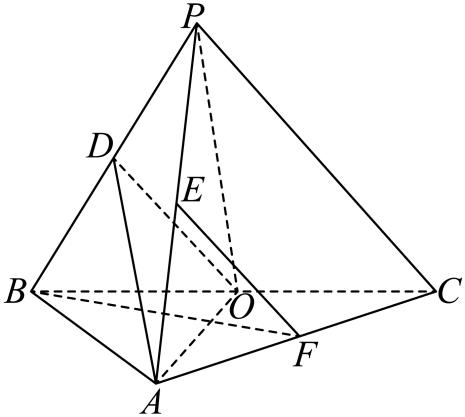
\includegraphics[width=.42\linewidth]{assets/asset-253-01.jpg}
\end{center}
\begin{choices}
  \item $\sqrt{5}$
  \item $3$
  \item $2\sqrt{5}$
  \item $5$
\end{choices}
\begin{solution}
\textbf{答案：}$3$

\textbf{分析：}方法一：以$\overrightarrow{AB},\overrightarrow{AD}$为基底向量表示$\overrightarrow{EC},\overrightarrow{ED}$，再结合数量积的运算律运算求解；方法二：建系，利用平面向量的坐标运算求解；方法三：利用余弦定理求$\cos\angle DEC$，进而根据数量积的定义运算求解.

\textbf{详解：}方法一：以$\overrightarrow{AB},\overrightarrow{AD}$为基底向量，可知$|\overrightarrow{AB}|=|\overrightarrow{AD}|=2$，$\overrightarrow{AB}\cdot\overrightarrow{AD}=0$，则$\overrightarrow{EC}=\overrightarrow{EB}+\overrightarrow{BC}=\frac{1}{2}\overrightarrow{AB}+\overrightarrow{AD}$，$\overrightarrow{ED}=\overrightarrow{EA}+\overrightarrow{AD}=-\frac{1}{2}\overrightarrow{AB}+\overrightarrow{AD}$，所以$\overrightarrow{EC}\cdot\overrightarrow{ED}=(\frac{1}{2}\overrightarrow{AB}+\overrightarrow{AD})\cdot(-\frac{1}{2}\overrightarrow{AB}+\overrightarrow{AD})=-\frac{1}{4}|\overrightarrow{AB}|^2+|\overrightarrow{AD}|^2=-1+4=3$；
方法二：如图，以$A$为坐标原点建立平面直角坐标系，则$E(1,0), C(2,2), D(0,2)$，可得$\overrightarrow{EC}=(1,2), \overrightarrow{ED}=(-1,2)$，所以$\overrightarrow{EC}\cdot\overrightarrow{ED}=-1+4=3$；
方法三：由题意可得$ED=EC=\sqrt{5}, CD=2$，在$\triangle CDE$中，由余弦定理得$\cos\angle DEC=\frac{DE^2+CE^2-DC^2}{2\cdot DE\cdot CE}=\frac{5+5-4}{2\times\sqrt{5}\times\sqrt{5}}=\frac{3}{5}$，所以$\overrightarrow{EC}\cdot\overrightarrow{ED}=|\overrightarrow{EC}||\overrightarrow{ED}|\cos\angle DEC=\sqrt{5}\times\sqrt{5}\times\frac{3}{5}=3$. 故选B.
\end{solution}
\end{question}

\begin{question}[points=5]
\textbf{来源：}2023 年 全国乙卷-文科，第 10 题\quad \textbf{专题：}三角函数\par
已知函数$f(x)=\sin(\omega x+\varphi)$在区间$(\frac{\pi}{6},\frac{2\pi}{3})$单调递增，直线$x=\frac{\pi}{6}$和$x=\frac{2\pi}{3}$为函数$y=f(x)$的图像的两条对称轴，则$f(-\frac{5\pi}{12})=$（   ）
\begin{choices}
  \item -$\frac{\sqrt{3}}{2}$
  \item -$\frac{1}{2}$
  \item $\frac{1}{2}$
  \item $\frac{\sqrt{3}}{2}$
\end{choices}
\begin{solution}
\textbf{答案：}$\frac{\sqrt{3}}{2}$

\textbf{分析：}根据题意分别求出其周期，再根据其最小值求出初相，代入$x=-\frac{5\pi}{12}$即可得到答案.

\textbf{详解：}因为$f(x)=\sin(\omega x+\varphi)$在区间$(\frac{\pi}{6},\frac{2\pi}{3})$单调递增，所以$\frac{T}{2}=\frac{2\pi}{3}-\frac{\pi}{6}=\frac{\pi}{2}$，且$\omega>0$，则$T=\pi$，$\omega=\frac{2\pi}{T}=2$，当$x=\frac{\pi}{6}$时，$f(x)$取得最小值，则$2\cdot\frac{\pi}{6}+\varphi=2k\pi-\frac{\pi}{2}$，$k\in \mathbb{Z}$，则$\varphi=2k\pi-\frac{5\pi}{6}$，$k\in \mathbb{Z}$，不妨取$k=0$，则$f(x)=\sin(2x-\frac{5\pi}{6})$，则$f(-\frac{5\pi}{12})=\sin(-\frac{5\pi}{3})=\frac{\sqrt{3}}{2}$. 故选D.
\end{solution}
\end{question}

\begin{question}[points=5]
\textbf{来源：}2023 年 全国乙卷-文科，第 14 题\quad \textbf{专题：}三角函数\par
若$\theta\in(0,\frac{\pi}{2})$，$\tan\theta=\frac{1}{2}$，则$\sin\theta-\cos\theta=$.
\fillin[{$-\frac{\sqrt{5}}{5}$}]
\begin{solution}
\textbf{答案：}$-\frac{\sqrt{5}}{5}$

\textbf{分析：}根据同角三角关系求$\sin\theta$，进而可得结果.

\textbf{详解：}因为$\theta\in(0,\frac{\pi}{2})$，则$\sin\theta>0, \cos\theta>0$，又因为$\tan\theta=\frac{\sin\theta}{\cos\theta}=\frac{1}{2}$，则$\cos\theta=2\sin\theta$，且$\cos^2\theta+\sin^2\theta=4\sin^2\theta+\sin^2\theta=5\sin^2\theta=1$，解得$\sin\theta=\frac{\sqrt{5}}{5}$或$\sin\theta=-\frac{\sqrt{5}}{5}$（舍去），所以$\sin\theta-\cos\theta=\sin\theta-2\sin\theta=-\sin\theta=-\frac{\sqrt{5}}{5}$. 故答案为$-\frac{\sqrt{5}}{5}$.
\end{solution}
\end{question}

\begin{question}[points=4]
\textbf{来源：}2023 年 上海卷，第 4 题\quad \textbf{专题：}三角函数\par
已知 $\tan \alpha = 2$，求 $\frac{\sin \alpha - \cos \alpha}{\sin \alpha + \cos \alpha}=$
\fillin[{$\frac{1}{3}$}]
\begin{solution}
\textbf{答案：}$\frac{1}{3}$
\end{solution}
\end{question}

\begin{question}[points=5]
\textbf{来源：}2023 年 上海卷，第 7 题\quad \textbf{专题：}三角形\par
已知 $\triangle ABC$ 的面积为 $\sqrt{3}$，$AB=2$，$AC=3$，求 $\angle A=$
\fillin[{$\frac{\pi}{3}$ 或 $\frac{2\pi}{3}$}]
\begin{solution}
\textbf{答案：}$\frac{\pi}{3}$ 或 $\frac{2\pi}{3}$
\end{solution}
\end{question}

\begin{question}[points=5]
\textbf{来源：}2023 年 上海卷，第 8 题\quad \textbf{专题：}三角形、三角函数\par
在 $\triangle ABC$ 中，$a=2$，$b=3$，$\cos C = \frac{1}{4}$，求 $c=$
\fillin[{$\sqrt{10}$}]
\begin{solution}
\textbf{答案：}$\sqrt{10}$
\end{solution}
\end{question}

\begin{question}[points=5]
\textbf{来源：}2023 年 上海卷，第 11 题\quad \textbf{专题：}三角函数\par
公园修建斜坡,假设斜坡起点在水平面上,斜坡与水平面的夹角为 $\theta$,斜坡终点距离水平面的垂直高度为4米,游客每走一米消耗的体能为 $1+\sin \theta$,要使游客从斜坡底走到斜坡顶端所消耗的总体能最少,则 $\tan \theta=$
\fillin[{$\frac{1}{2}$}]
\begin{solution}
\textbf{答案：}$\frac{1}{2}$
\end{solution}
\end{question}

\begin{question}[points=5]
\textbf{来源：}2023 年 上海卷，第 16 题\quad \textbf{专题：}向量\par
在平面上,若曲线 $C$ 具有如下性质:存在点 $P$,使得对于任意点 $Q\in C$,都有 $R\in C$ 使得 $\overrightarrow{PQ}+\overrightarrow{PR}=0$.则称这条曲线为"自相关曲线".判断下列两个命题的真假().(1)所有椭圆都是"自相关曲线".(2)存在是"自相关曲线"的双曲线.
\begin{choices}
  \item (1)假命题；(2)真命题
  \item (1)真命题；(2)假命题
  \item (1)真命题；(2)真命题
  \item (1)假命题；(2)假命题
\end{choices}
\begin{solution}
\textbf{答案：}B
\end{solution}
\end{question}

\begin{question}[points=5]
\textbf{来源：}2023 年 天津卷，第 4 题\quad \textbf{专题：}三角函数\par
函数 $f(x)$ 的图象如下图所示, 则 $f(x)$ 的解析式可能为 ( )

\begin{center}
  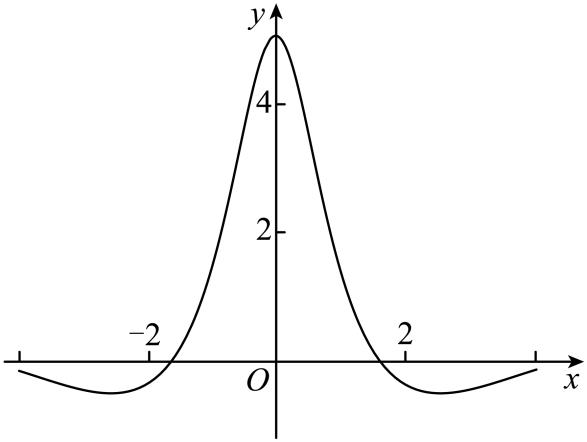
\includegraphics[width=.42\linewidth]{assets/asset-261-01.jpg}
\end{center}
\begin{choices}
  \item $\dfrac{5(e^x - e^{-x})}{x^2 + 2}$
  \item $\dfrac{5\sin x}{x^2 + 1}$
  \item $\dfrac{5(e^x + e^{-x})}{x^2 + 2}$
  \item $\dfrac{5\cos x}{x^2 + 1}$
\end{choices}
\begin{solution}
\textbf{答案：}D

\textbf{分析：}由图知函数为偶函数, 应用排除法.

\textbf{详解：}由图知: 函数图象关于 $y$ 轴对称, 其为偶函数, 且 $f(-2) = f(2) < 0$. 由 $\dfrac{5\sin(-x)}{(-x)^2 + 1} = -\dfrac{5\sin x}{x^2 + 1}$ 且定义域为 $\mathbb{R}$, 即 B 中函数为奇函数, 排除. 当 $x > 0$ 时 $\dfrac{5(e^x - e^{-x})}{x^2 + 2} > 0$, $\dfrac{5(e^x + e^{-x})}{x^2 + 2} > 0$, 即 A、C 中 $(0, +\infty)$ 上函数值为正, 排除. 故选 D.
\end{solution}
\end{question}

\begin{question}[points=5]
\textbf{来源：}2023 年 天津卷，第 5 题\quad \textbf{专题：}三角函数\par
已知函数 $f(x)$ 的一条对称轴为直线 $x = 2$, 一个周期为 $4$, 则 $f(x)$ 的解析式可能为 ( )
\begin{choices}
  \item $\sin\left(\dfrac{\pi}{2}x\right)$
  \item $\cos\left(\dfrac{\pi}{2}x\right)$
  \item $\sin\left(\dfrac{\pi}{4}x\right)$
  \item $\cos\left(\dfrac{\pi}{4}x\right)$
\end{choices}
\begin{solution}
\textbf{答案：}B

\textbf{分析：}由题意分别考查函数的最小正周期和函数在 $x=2$ 处的函数值.

\textbf{详解：}A 选项 $T = \dfrac{2\pi}{\pi/2} = 4$, B 选项 $T = \dfrac{2\pi}{\pi/2} = 4$, C 选项 $T = \dfrac{2\pi}{\pi/4} = 8$, D 选项 $T = \dfrac{2\pi}{\pi/4} = 8$, 排除 CD. 对于 A, 当 $x=2$ 时 $\sin\left(\dfrac{\pi}{2}\cdot 2\right)=0$, 故 $(2,0)$ 是一个对称中心, 排除 A. 对于 B, 当 $x=2$ 时 $\cos\left(\dfrac{\pi}{2}\cdot 2\right) = -1$, 故 $x=2$ 是一条对称轴. 故选 B.
\end{solution}
\end{question}

\begin{question}[points=5]
\textbf{来源：}2023 年 天津卷，第 14 题\quad \textbf{专题：}向量、三角形\par
在 $\triangle ABC$ 中，$\angle A = 60^\circ$，$BC = 1$，点 $D$ 为 $AB$ 的中点，点 $E$ 为 $CD$ 的中点，若设 $\overrightarrow{AB} = \vec{a}$，$\overrightarrow{AC} = \vec{b}$，则 $\overrightarrow{AE}$ 可用 $\vec{a}, \vec{b}$ 表示为；若 $\overrightarrow{BF} = \dfrac{1}{3} \overrightarrow{BC}$，则 $\overrightarrow{AE} \cdot \overrightarrow{AF}$ 的最大值为．
\fillin[{$\dfrac{1}{4}\vec{a} + \dfrac{1}{2}\vec{b}$ ; $\dfrac{13}{24}$}]
\begin{solution}
\textbf{答案：}$\dfrac{1}{4}\vec{a} + \dfrac{1}{2}\vec{b}$ ; $\dfrac{13}{24}$

\textbf{分析：}利用向量线性运算和数量积，结合余弦定理和基本不等式.

\textbf{详解：}因为 $E$ 为 $CD$ 的中点，则 $\overrightarrow{ED} + \overrightarrow{EC} = \vec{0}$，由 $\begin{cases} \overrightarrow{AE} + \overrightarrow{ED} = \overrightarrow{AD} \\ \overrightarrow{AE} + \overrightarrow{EC} = \overrightarrow{AC} \end{cases}$ 两式相加得 $2\overrightarrow{AE} = \overrightarrow{AD} + \overrightarrow{AC} = \dfrac{1}{2}\overrightarrow{AB} + \overrightarrow{AC} = \dfrac{1}{2}\vec{a} + \vec{b}$，所以 $\overrightarrow{AE} = \dfrac{1}{4}\vec{a} + \dfrac{1}{2}\vec{b}$. 因为 $\overrightarrow{BF} = \dfrac{1}{3}\overrightarrow{BC}$，则 $2\overrightarrow{FB} + \overrightarrow{FC} = \vec{0}$，由 $\begin{cases} \overrightarrow{AF} + \overrightarrow{FC} = \overrightarrow{AC} \\ \overrightarrow{AF} + \overrightarrow{FB} = \overrightarrow{AB} \end{cases}$ 两式相加得 $3\overrightarrow{AF} = 2\overrightarrow{AB} + \overrightarrow{AC} = 2\vec{a} + \vec{b}$，所以 $\overrightarrow{AF} = \dfrac{2}{3}\vec{a} + \dfrac{1}{3}\vec{b}$. 所以 $\overrightarrow{AE} \cdot \overrightarrow{AF} = \left(\dfrac{1}{4}\vec{a} + \dfrac{1}{2}\vec{b}\right) \cdot \left(\dfrac{2}{3}\vec{a} + \dfrac{1}{3}\vec{b}\right) = \dfrac{1}{12}(2|\vec{a}|^2 + 5\vec{a}\cdot\vec{b} + 2|\vec{b}|^2)$. 设 $AB = x$, $AC = y$, 则 $\vec{a}\cdot\vec{b} = xy\cos60^\circ = \dfrac{xy}{2}$, 且 $BC^2 = x^2 + y^2 - xy = 1$, 所以 $2x^2 + 5\cdot\frac{xy}{2} + 2y^2 = 2(x^2 + y^2) + \frac{5}{2}xy = 2(1+xy) + \frac{5}{2}xy = 2 + \frac{9}{2}xy$. 由 $x^2 + y^2 \ge 2xy$ 得 $1 = x^2 + y^2 - xy \ge xy$, 即 $xy \le 1$, 当 $x = y = 1$ 时取等. 所以 $\overrightarrow{AE} \cdot \overrightarrow{AF} = \dfrac{1}{12}\left(2 + \frac{9}{2}xy\right) \le \dfrac{1}{12}\left(2 + \frac{9}{2}\right) = \dfrac{13}{24}$.
\end{solution}
\end{question}

\begin{question}[points=14]
\textbf{来源：}2023 年 天津卷，第 16 题\quad \textbf{专题：}三角形、三角函数\par
在 $\triangle ABC$ 中，角 $A, B, C$ 所对的边分别是 $a, b, c$．已知 $a = \sqrt{39}$, $b = 2$, $\angle A = 120^\circ$．

(1) 求 $\sin B$ 的值；

(2) 求 $c$ 的值；

(3) 求 $\sin(B - C)$．
\begin{solution}
\textbf{答案：}(1) $\dfrac{\sqrt{13}}{13}$ ; (2) $5$ ; (3) $-\dfrac{7\sqrt{3}}{26}$

\textbf{详解：}(1) 由正弦定理 $\dfrac{a}{\sin A} = \dfrac{b}{\sin B}$, 得 $\dfrac{\sqrt{39}}{\sin120^\circ} = \dfrac{2}{\sin B}$, 解得 $\sin B = \dfrac{\sqrt{13}}{13}$.
(2) 由余弦定理 $a^2 = b^2 + c^2 - 2bc\cos A$, 即 $39 = 4 + c^2 - 2\cdot 2 \cdot c \cdot \left(-\frac{1}{2}\right) = 4 + c^2 + 2c$, 整理得 $c^2 + 2c - 35 = 0$, 解得 $c = 5$ (负值舍去).
(3) 由正弦定理 $\dfrac{a}{\sin A} = \dfrac{c}{\sin C}$ 得 $\dfrac{\sqrt{39}}{\sin120^\circ} = \dfrac{5}{\sin C}$, 解得 $\sin C = \dfrac{5\sqrt{13}}{26}$. 因为 $A = 120^\circ$, 所以 $B, C$ 均为锐角, $\cos B = \sqrt{1-\left(\frac{\sqrt{13}}{13}\right)^2} = \dfrac{2\sqrt{39}}{13}$, $\cos C = \sqrt{1-\left(\frac{5\sqrt{13}}{26}\right)^2} = \dfrac{\sqrt{39}}{26}$. 所以 $\sin(B-C) = \sin B \cos C - \cos B \sin C = \dfrac{\sqrt{13}}{13} \cdot \dfrac{\sqrt{39}}{26} - \dfrac{2\sqrt{39}}{13} \cdot \dfrac{5\sqrt{13}}{26} = -\dfrac{7\sqrt{3}}{26}$.
\end{solution}
\end{question}

\begin{question}[points=5]
\textbf{来源：}2023 年 新高考II卷，第 5 题\quad \textbf{专题：}三角形\par
已知椭圆$C:\dfrac{x^{2}}{3}+y^{2}=1$的左、右焦点分别为$F_{1}$，$F_{2}$，直线$y=x+m$与$C$交于$A$，$B$两点，若$\triangle F_{1}AB$面积是$\triangle F_{2}AB$面积的2倍，则$m=$（ \quad ）
\begin{choices}
  \item A. $\dfrac{2}{3}$
  \item B. $\dfrac{\sqrt{2}}{3}$
  \item C. $-\dfrac{2}{3}$
  \item D. $-\dfrac{\sqrt{2}}{3}$
\end{choices}
\begin{solution}
\textbf{答案：}C

\textbf{分析：}首先联立直线方程与椭圆方程，利用$\Delta>0$，求出$m$范围，再根据三角形面积比得到关于$m$的方程，解出即可.

\textbf{详解：}将直线$y=x+m$与椭圆联立$\begin{cases}y=x+m\\ \dfrac{x^{2}}{3}+y^{2}=1\end{cases}$，消去$y$可得$4x^{2}+6mx+3m^{2}-3=0$，因为直线与椭圆相交于$A,B$点，则$\Delta=36m^{2}-4\times4(3m^{2}-3)>0$，解得$-2<m<2$，设$F_{1}$到$AB$的距离$d_{1}$，$F_{2}$到$AB$的距离$d_{2}$，易知$F_{1}(-\sqrt{2},0),F_{2}(\sqrt{2},0)$，则$d_{1}=\dfrac{|-\sqrt{2}+m|}{\sqrt{2}}$，$d_{2}=\dfrac{|\sqrt{2}+m|}{\sqrt{2}}$，$\dfrac{S_{\triangle F_{1}AB}}{S_{\triangle F_{2}AB}}=\dfrac{|\sqrt{2}+m|}{|\sqrt{2}-m|}=2$，解得$m=-\dfrac{2}{3}$或$-3\sqrt{2}$（舍去）.
\end{solution}
\end{question}

\begin{question}[points=5]
\textbf{来源：}2023 年 新高考II卷，第 7 题\quad \textbf{专题：}三角函数\par
已知$\alpha$为锐角，$\cos\alpha=\dfrac{1+\sqrt{5}}{4}$，则$\sin\dfrac{\alpha}{2}=$（ \quad ）
\begin{choices}
  \item A. $\dfrac{3-\sqrt{5}}{8}$
  \item B. $\dfrac{-1+\sqrt{5}}{8}$
  \item C. $\dfrac{3-\sqrt{5}}{4}$
  \item D. $\dfrac{-1+\sqrt{5}}{4}$
\end{choices}
\begin{solution}
\textbf{答案：}D

\textbf{分析：}根据二倍角公式（或者半角公式）即可求出.

\textbf{详解：}因为$\cos\alpha=1-2\sin^{2}\dfrac{\alpha}{2}=\dfrac{1+\sqrt{5}}{4}$，而$\alpha$为锐角，解得$\sin\dfrac{\alpha}{2}=\dfrac{3-\sqrt{5}}{8}=\dfrac{(\sqrt{5}-1)^{2}}{16}=\dfrac{\sqrt{5}-1}{4}$.
\end{solution}
\end{question}

\begin{question}[points=5]
\textbf{来源：}2023 年 新高考II卷，第 9 题\quad \textbf{专题：}三角形\par
已知圆锥的顶点为$P$，底面圆心为$O$，$AB$为底面直径，$\angle APB=120^{\circ}$，$PA=2$，点$C$在底面圆周上，且二面角$P-AC-O$为$45^{\circ}$，则（ \quad ）
\begin{choices}
  \item A. 该圆锥的体积为$\pi$
  \item B. 该圆锥的侧面积为$4\sqrt{3}\pi$
  \item C. $AC=2\sqrt{2}$
  \item D. $\triangle PAC$的面积为$\sqrt{3}$
\end{choices}
\begin{solution}
\textbf{答案：}AC

\textbf{分析：}根据圆锥的体积、侧面积判断A、B选项的正确性，利用二面角的知识判断C、D选项的正确性.

\textbf{详解：}依题意，$\angle APB=120^{\circ}$，$PA=2$，所以$OP=1$，$OA=OB=\sqrt{3}$；A选项，圆锥的体积为$\dfrac{1}{3}\times\pi\times(\sqrt{3})^{2}\times1=\pi$，A正确；B选项，圆锥的侧面积为$\pi\times\sqrt{3}\times2=2\sqrt{3}\pi$，B错误；C选项，设$D$是$AC$的中点，连接$OD,PD$，则$AC\perp OD$，$AC\perp PD$，所以$\angle PDO$是二面角$P-AC-O$的平面角，则$\angle PDO=45^{\circ}$，所以$OP=OD=1$，故$AD=CD=\sqrt{3-1}=\sqrt{2}$，则$AC=2\sqrt{2}$，C正确；D选项，$PD=\sqrt{1^{2}+1^{2}}=\sqrt{2}$，所以$S_{\triangle PAC}=\dfrac{1}{2}\times2\sqrt{2}\times\sqrt{2}=2$，D错误.
\end{solution}
\end{question}

\begin{question}[points=5]
\textbf{来源：}2023 年 新高考II卷，第 13 题\quad \textbf{专题：}向量\par
已知向量$\vec{a}$，$\vec{b}$满足$|\vec{a}-\vec{b}|=\sqrt{3}$，$|\vec{a}+\vec{b}|=|2\vec{a}-\vec{b}|$，则$|\vec{b}|=$ ．
\fillin[{$\sqrt{3}$}]
\begin{solution}
\textbf{答案：}$\sqrt{3}$

\textbf{分析：}法一：根据题意结合向量数量积的运算律运算求解；法二：换元令$\vec{c}=\vec{a}-\vec{b}$，结合数量积的运算律运算求解.

\textbf{详解：}法一：因为$|\vec{a}+\vec{b}|=|2\vec{a}-\vec{b}|$，即$(\vec{a}+\vec{b})^{2}=(2\vec{a}-\vec{b})^{2}$，则$\vec{a}^{2}+2\vec{a}\cdot\vec{b}+\vec{b}^{2}=4\vec{a}^{2}-4\vec{a}\cdot\vec{b}+\vec{b}^{2}$，整理得$\vec{a}^{2}-2\vec{a}\cdot\vec{b}=0$，又因为$|\vec{a}-\vec{b}|=\sqrt{3}$，即$(\vec{a}-\vec{b})^{2}=3$，则$\vec{a}^{2}-2\vec{a}\cdot\vec{b}+\vec{b}^{2}=|\vec{b}|^{2}=3$，所以$|\vec{b}|=\sqrt{3}$.
法二：设$\vec{c}=\vec{a}-\vec{b}$，则$|\vec{c}|=\sqrt{3}$，$\vec{a}+\vec{b}=\vec{c}+2\vec{b}$，$2\vec{a}-\vec{b}=2\vec{c}+\vec{b}$，由题意可得$(\vec{c}+2\vec{b})^{2}=(2\vec{c}+\vec{b})^{2}$，则$\vec{c}^{2}+4\vec{c}\cdot\vec{b}+4\vec{b}^{2}=4\vec{c}^{2}+4\vec{c}\cdot\vec{b}+\vec{b}^{2}$，整理得$\vec{c}^{2}=\vec{b}^{2}$，即$|\vec{b}|=|\vec{c}|=\sqrt{3}$.
\end{solution}
\end{question}

\begin{question}[points=5]
\textbf{来源：}2023 年 新高考II卷，第 15 题\quad \textbf{专题：}三角形\par
已知直线$l:x-my+1=0$与$\odot C:(x-1)^{2}+y^{2}=4$交于$A$，$B$两点，写出满足“$\triangle ABC$面积为$\dfrac{8}{5}$”的$m$的一个值．
\fillin[{2（$\pm2$或$\pm\dfrac{1}{2}$中任意一个皆可以）}]
\begin{solution}
\textbf{答案：}2（$\pm2$或$\pm\dfrac{1}{2}$中任意一个皆可以）

\textbf{分析：}根据直线与圆的位置关系，求出弦长$AB$，以及点$C$到直线$AB$的距离，结合面积公式即可解出.

\textbf{详解：}设点$C$到直线$AB$的距离为$d$，由弦长公式得$|AB|=2\sqrt{4-d^{2}}$，所以$S_{\triangle ABC}=\dfrac{1}{2}\times d\times2\sqrt{4-d^{2}}=\dfrac{8}{5}$，解得$d=\dfrac{4\sqrt{5}}{5}$或$d=\dfrac{2\sqrt{5}}{5}$，由$d=\dfrac{|1+1|}{\sqrt{1+m^{2}}}=\dfrac{2}{\sqrt{1+m^{2}}}$，所以$\dfrac{2}{\sqrt{1+m^{2}}}=\dfrac{4\sqrt{5}}{5}$或$\dfrac{2}{\sqrt{1+m^{2}}}=\dfrac{2\sqrt{5}}{5}$，解得$m=\pm2$或$m=\pm\dfrac{1}{2}$，故填写其中一个即可.
\end{solution}
\end{question}

\begin{question}[points=5]
\textbf{来源：}2023 年 新高考II卷，第 16 题\quad \textbf{专题：}三角函数\par
已知函数$f(x)=\sin(\omega x+\varphi)$，如图$A$，$B$是直线$y=\dfrac{1}{2}$与曲线$y=f(x)$的两个交点，若$|AB|=\dfrac{\pi}{6}$，则$f(\pi)=$ ．

\begin{center}
  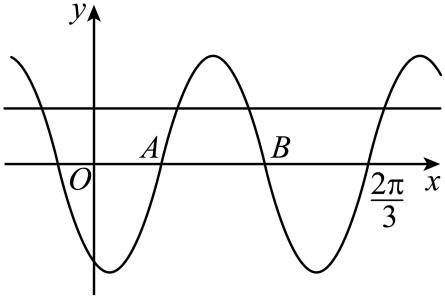
\includegraphics[width=.42\linewidth]{assets/asset-270-01.jpg}
\end{center}
\fillin[{$-\dfrac{\sqrt{3}}{2}$}]
\begin{solution}
\textbf{答案：}$-\dfrac{\sqrt{3}}{2}$

\textbf{分析：}设$A\left(x_{1},\dfrac{1}{2}\right),B\left(x_{2},\dfrac{1}{2}\right)$，依题可得$x_{2}-x_{1}=\dfrac{\pi}{6}$，结合$\sin x=\dfrac{1}{2}$的解可得$\omega(x_{2}-x_{1})=\dfrac{2\pi}{3}$，从而得到$\omega$的值，再根据$f\left(\dfrac{2\pi}{3}\right)=0$以及$f(0)<0$，即可得$f(x)=\sin\left(4x-\dfrac{2\pi}{3}\right)$，进而求得$f(\pi)$.

\textbf{详解：}设$A\left(x_{1},\dfrac{1}{2}\right),B\left(x_{2},\dfrac{1}{2}\right)$，由$|AB|=\dfrac{\pi}{6}$可得$x_{2}-x_{1}=\dfrac{\pi}{6}$，由$\sin x=\dfrac{1}{2}$可知，$x=\dfrac{\pi}{6}+2k\pi$或$x=\dfrac{5\pi}{6}+2k\pi$，$k\in\mathbb{Z}$，由图可知，$\omega x_{2}+\varphi-(\omega x_{1}+\varphi)=\dfrac{5\pi}{6}-\dfrac{\pi}{6}=\dfrac{2\pi}{3}$，即$\omega(x_{2}-x_{1})=\dfrac{2\pi}{3}$，$\therefore\omega=4$. 因为$f\left(\dfrac{2\pi}{3}\right)=\sin\left(\dfrac{8\pi}{3}+\varphi\right)=0$，所以$\dfrac{8\pi}{3}+\varphi=k\pi$，即$\varphi=-\dfrac{8\pi}{3}+k\pi$，$k\in\mathbb{Z}$. 所以$f(x)=\sin\left(4x-\dfrac{8\pi}{3}+k\pi\right)=\sin\left(4x-\dfrac{2\pi}{3}+k\pi\right)$，所以$f(x)=\sin\left(4x-\dfrac{2\pi}{3}\right)$或$f(x)=-\sin\left(4x-\dfrac{2\pi}{3}\right)$，又因为$f(0)<0$，所以$f(x)=\sin\left(4x-\dfrac{2\pi}{3}\right)$，$\therefore f(\pi)=\sin\left(4\pi-\dfrac{2\pi}{3}\right)=-\dfrac{\sqrt{3}}{2}$.
\end{solution}
\end{question}

\begin{question}[points=10]
\textbf{来源：}2023 年 新高考II卷，第 17 题\quad \textbf{专题：}三角形、三角函数\par
记$\triangle ABC$的内角$A,B,C$的对边分别为$a,b,c$，已知$\triangle ABC$的面积为$\sqrt{3}$，$D$为$BC$中点，且$AD=1$．

（1）若$\angle ADC=\dfrac{\pi}{3}$，求$\tan B$；

（2）若$b^{2}+c^{2}=8$，求$b,c$．
\begin{solution}
\textbf{答案：}（1）$\dfrac{\sqrt{3}}{5}$；（2）$b=c=2$.

\textbf{分析：}（1）方法1，利用三角形面积公式求出$a$，再利用余弦定理求解作答；方法2，利用三角形面积公式求出$a$，作出$BC$边上的高，利用直角三角形求解作答.
（2）方法1，利用余弦定理求出$a$，再利用三角形面积公式求出$\angle ADC$即可求解作答；方法2，利用向量运算律建立关系求出$a$，再利用三角形面积公式求出$\angle ADC$即可求解作答.

\textbf{详解：}（1）方法1：在$\triangle ABC$中，因为$D$为$BC$中点，$\angle ADC=\dfrac{\pi}{3}$，$AD=1$，则$S_{\triangle ADC}=\dfrac{1}{2}AD\cdot DC\sin\angle ADC=\dfrac{1}{2}\times1\times\dfrac{a}{2}\times\dfrac{\sqrt{3}}{2}=\dfrac{\sqrt{3}}{8}a=\dfrac{1}{2}S_{\triangle ABC}=\dfrac{\sqrt{3}}{2}$，解得$a=4$，在$\triangle ABD$中，$\angle ADB=\dfrac{2\pi}{3}$，由余弦定理得$c^{2}=BD^{2}+AD^{2}-2BD\cdot AD\cos\angle ADB$，即$c^{2}=4+1-2\times2\times1\times(-\dfrac{1}{2})=7$，解得$c=\sqrt{7}$，则$\cos B=\dfrac{7+4-1}{2\times\sqrt{7}\times2}=\dfrac{5\sqrt{7}}{14}$，$\sin B=\sqrt{1-\cos^{2}B}=\sqrt{1-\left(\dfrac{5\sqrt{7}}{14}\right)^{2}}=\dfrac{\sqrt{21}}{14}$，所以$\tan B=\dfrac{\sin B}{\cos B}=\dfrac{\sqrt{3}}{5}$.
方法2：在$\triangle ABC$中，因为$D$为$BC$中点，$\angle ADC=\dfrac{\pi}{3}$，$AD=1$，则$S_{\triangle ADC}=\dfrac{1}{2}AD\cdot DC\sin\angle ADC=\dfrac{1}{2}\times1\times\dfrac{a}{2}\times\dfrac{\sqrt{3}}{2}=\dfrac{\sqrt{3}}{8}a=\dfrac{1}{2}S_{\triangle ABC}=\dfrac{\sqrt{3}}{2}$，解得$a=4$，在$\triangle ACD$中，由余弦定理得$b^{2}=CD^{2}+AD^{2}-2CD\cdot AD\cos\angle ADC$，即$b^{2}=4+1-2\times2\times1\times\dfrac{1}{2}=3$，解得$b=\sqrt{3}$，有$AC^{2}+AD^{2}=4=CD^{2}$，则$\angle CAD=\dfrac{\pi}{2}$，$\angle C=\dfrac{\pi}{6}$，过$A$作$AE\perp BC$于$E$，于是$CE=AC\cos C=\dfrac{3}{2}$，$AE=AC\sin C=\dfrac{\sqrt{3}}{2}$，$BE=\dfrac{5}{2}$，所以$\tan B=\dfrac{AE}{BE}=\dfrac{\sqrt{3}}{5}$.
（2）方法1：在$\triangle ABD$与$\triangle ACD$中，由余弦定理得$\begin{cases}c^{2}=\dfrac{1}{4}a^{2}+1-2\times\dfrac{a}{2}\times1\times\cos(\pi-\angle ADC)\\ b^{2}=\dfrac{1}{4}a^{2}+1-2\times\dfrac{a}{2}\times1\times\cos\angle ADC\end{cases}$，整理得$\dfrac{1}{2}a^{2}+2=b^{2}+c^{2}$，而$b^{2}+c^{2}=8$，则$a=2\sqrt{3}$，又$S_{\triangle ADC}=\dfrac{1}{2}\times\sqrt{3}\times1\times\sin\angle ADC=\dfrac{\sqrt{3}}{2}$，解得$\sin\angle ADC=1$，而$0<\angle ADC<\pi$，于是$\angle ADC=\dfrac{\pi}{2}$，所以$b=c=\sqrt{AD^{2}+CD^{2}}=2$.
方法2：在$\triangle ABC$中，因为$D$为$BC$中点，则$2\overrightarrow{AD}=\overrightarrow{AB}+\overrightarrow{AC}$，又$\overrightarrow{CB}=\overrightarrow{AB}-\overrightarrow{AC}$，于是$4|\overrightarrow{AD}|^{2}+|\overrightarrow{CB}|^{2}=(\overrightarrow{AB}+\overrightarrow{AC})^{2}+(\overrightarrow{AB}-\overrightarrow{AC})^{2}=2(b^{2}+c^{2})=16$，即$4+a^{2}=16$，解得$a=2\sqrt{3}$，又$S_{\triangle ADC}=\dfrac{1}{2}\times\sqrt{3}\times1\times\sin\angle ADC=\dfrac{\sqrt{3}}{2}$，解得$\sin\angle ADC=1$，而$0<\angle ADC<\pi$，于是$\angle ADC=\dfrac{\pi}{2}$，所以$b=c=\sqrt{AD^{2}+CD^{2}}=2$.
\end{solution}
\end{question}

\begin{question}[points=10]
\textbf{来源：}2023 年 新高考II卷，第 20 题\quad \textbf{专题：}向量\par
如图，三棱锥$A-BCD$中，$DA=DB=DC$，$BD\perp CD$，$\angle ADB=\angle ADC=60^{\circ}$，$E$为$BC$的中点．

（1）证明：$BC\perp DA$；

（2）点$F$满足$\overrightarrow{EF}=\overrightarrow{DA}$，求二面角$D-AB-F$的正弦值．

\begin{center}
  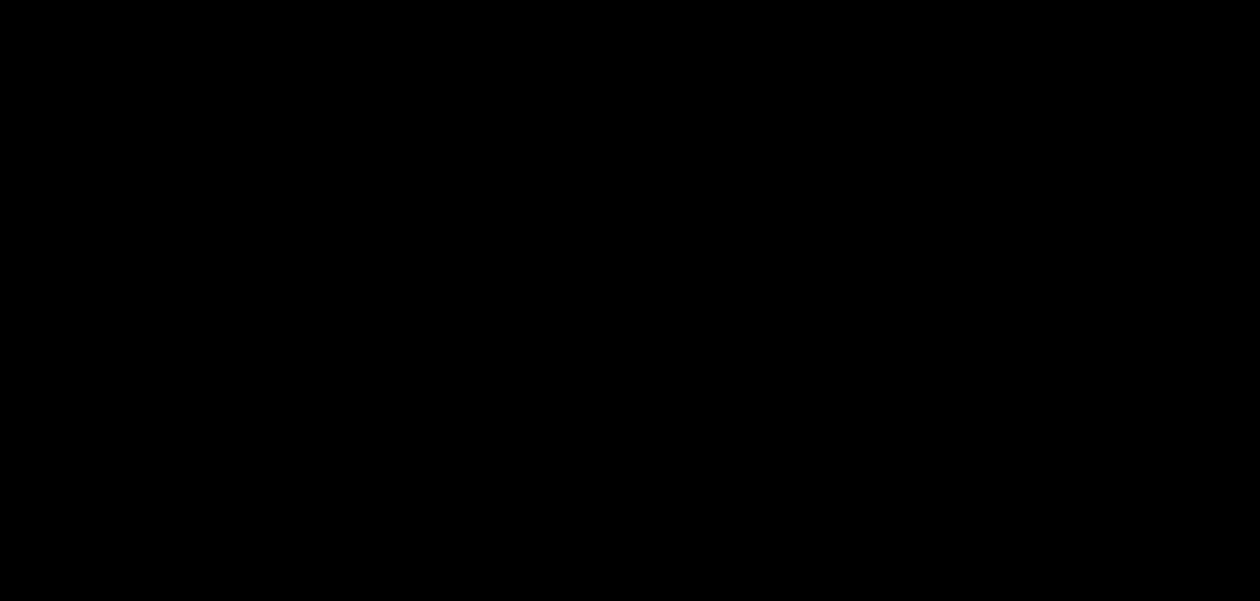
\includegraphics[width=.42\linewidth]{assets/asset-272-01.jpg}
\end{center}
\begin{solution}
\textbf{答案：}（1）证明见解析；（2）$\dfrac{\sqrt{3}}{3}$.

\textbf{分析：}（1）根据题意易证$BC\perp$平面$ADE$，从而证得$BC\perp DA$；
（2）由题可证$AE\perp$平面$BCD$，所以以点$E$为原点，$ED,EB,EA$所在直线分别为$x,y,z$轴，建立空间直角坐标系，再求出平面$ABD$，$ABF$的一个法向量，根据二面角的向量公式以及同角三角函数关系即可解出.

\textbf{详解：}（1）连接$AE,DE$，因为$E$为$BC$中点，$DB=DC$，所以$DE\perp BC$①，因为$DA=DB=DC$，$\angle ADB=\angle ADC=60^{\circ}$，所以$\triangle ACD$与$\triangle ABD$均为等边三角形，$\therefore AC=AB$，从而$AE\perp BC$②，由①②，$AE\cap DE=E$，$AE,DE\subset$平面$ADE$，所以$BC\perp$平面$ADE$，而$AD\subset$平面$ADE$，所以$BC\perp DA$.
（2）不妨设$DA=DB=DC=2$，$\because BD\perp CD$，$\therefore BC=2\sqrt{2}$，$DE=AE=\sqrt{2}$，$\because AE^{2}+DE^{2}=4=AD^{2}$，$\therefore AE\perp DE$，又$\because AE\perp BC$，$DE\cap BC=E$，$DE,BC\subset$平面$BCD$，$\therefore AE\perp$平面$BCD$．以点$E$为原点，$ED,EB,EA$所在直线分别为$x,y,z$轴，建立空间直角坐标系，如图所示：
设$D(\sqrt{2},0,0)$，$A(0,0,\sqrt{2})$，$B(0,\sqrt{2},0)$，$E(0,0,0)$，设平面$DAB$与平面$ABF$的一个法向量分别为$\vec{n_{1}}=(x_{1},y_{1},z_{1})$，$\vec{n_{2}}=(x_{2},y_{2},z_{2})$，二面角$D-AB-F$平面角为$\theta$，而$\overrightarrow{AB}=(0,\sqrt{2},-\sqrt{2})$，因为$\overrightarrow{EF}=\overrightarrow{DA}=(-\sqrt{2},0,\sqrt{2})$，所以$F(-\sqrt{2},0,\sqrt{2})$，即有$\overrightarrow{AF}=(-\sqrt{2},0,0)$，$\therefore\begin{cases}-\sqrt{2}x_{1}+\sqrt{2}z_{1}=0\\ \sqrt{2}y_{1}-\sqrt{2}z_{1}=0\end{cases}$，取$x_{1}=1$，所以$\vec{n_{1}}=(1,1,1)$；$\begin{cases}\sqrt{2}y_{2}-\sqrt{2}z_{2}=0\\ -\sqrt{2}x_{2}=0\end{cases}$，取$y_{2}=1$，所以$\vec{n_{2}}=(0,1,1)$，所以$\cos\theta=\dfrac{\vec{n_{1}}\cdot\vec{n_{2}}}{|\vec{n_{1}}||\vec{n_{2}}|}=\dfrac{2}{\sqrt{3}\times\sqrt{2}}=\dfrac{\sqrt{6}}{3}$，从而$\sin\theta=\sqrt{1-\dfrac{6}{9}}=\dfrac{\sqrt{3}}{3}$，所以二面角$D-AB-F$的正弦值为$\dfrac{\sqrt{3}}{3}$.
\end{solution}
\end{question}

\begin{question}[points=10]
\textbf{来源：}2023 年 新高考II卷，第 22 题\quad \textbf{专题：}三角函数\par
（1）证明：当$0<x<1$时，$x-x^{2}<\sin x<x$；

（2）已知函数$f(x)=\cos ax-\ln(1-x^{2})$，若$x=0$是$f(x)$的极大值点，求$a$的取值范围．
\begin{solution}
\textbf{答案：}（1）证明见详解；（2）$(-\infty,-\sqrt{2})\cup(\sqrt{2},+\infty)$.

\textbf{分析：}（1）分别构建$F(x)=x-\sin x$，$x\in(0,1)$，$G(x)=x-x^{2}+\sin x$，$x\in(0,1)$，求导，利用导数判断原函数的单调性，进而可得结果；
（2）根据题意结合偶函数的性质可知只需要研究$f(x)$在$(0,1)$上的单调性，求导，分类讨论$0<a^{2}\le 2$和$a^{2}\ge 2$，结合（1）中的结论放缩，根据极大值的定义分析求解.

\textbf{详解：}（1）构建$F(x)=x-\sin x$，$x\in(0,1)$，则$F'(x)=1-\cos x>0$对$\forall x\in(0,1)$恒成立，则$F(x)$在$(0,1)$上单调递增，可得$F(x)>F(0)=0$，所以$x>\sin x$，$x\in(0,1)$；构建$G(x)=\sin x-(x-x^{2})=x-x^{2}+\sin x$，$x\in(0,1)$，则$G'(x)=2x-1+\cos x$，$x\in(0,1)$，构建$g(x)=G'(x)$，$x\in(0,1)$，则$g'(x)=2-\sin x>0$对$\forall x\in(0,1)$恒成立，则$g(x)$在$(0,1)$上单调递增，可得$g(x)>g(0)=0$，即$G'(x)>0$对$\forall x\in(0,1)$恒成立，则$G(x)$在$(0,1)$上单调递增，可得$G(x)>G(0)=0$，所以$\sin x>x-x^{2}$，$x\in(0,1)$；综上所述：$x-x^{2}<\sin x<x$.
（2）令$1-x^{2}>0$，解得$-1<x<1$，即函数$f(x)$的定义域为$(-1,1)$，若$a=0$，则$f(x)=-\ln(1-x^{2})$，$x\in(-1,1)$，因为$y=-\ln u$在定义域内单调递减，$y=1-x^{2}$在$(-1,0)$上单调递增，在$(0,1)$上单调递减，则$f(x)=-\ln(1-x^{2})$在$(-1,0)$上单调递减，在$(0,1)$上单调递增，故$x=0$是$f(x)$的极小值点，不合题意，所以$a\neq0$.
当$a\neq0$时，令$b=|a|>0$，因为$f(x)=\cos ax-\ln(1-x^{2})=\cos(|a|x)-\ln(1-x^{2})=\cos bx-\ln(1-x^{2})$，且$f(-x)=\cos(-bx)-\ln[1-(-x)^{2}]=\cos bx-\ln(1-x^{2})=f(x)$，所以函数$f(x)$在定义域内为偶函数，由题意可得：$f'(x)=-b\sin bx-\dfrac{2x}{x^{2}-1}$，$x\in(-1,1)$.
（i）当$0<b^{2}\le 2$时，取$m=\min\{\dfrac{1}{b},1\}$，$x\in(0,m)$，则$bx\in(0,1)$，由（1）可得$f'(x)=-b\sin(bx)-\dfrac{2x}{x^{2}-1}>-b^{2}x-\dfrac{2x}{x^{2}-1}=\dfrac{x(b^{2}x^{2}+2-b^{2})}{1-x^{2}}$，且$b^{2}x^{2}>0$，$2-b^{2}\ge0$，$1-x^{2}>0$，所以$f'(x)>\dfrac{x(b^{2}x^{2}+2-b^{2})}{1-x^{2}}>0$，即当$x\in(0,m)\subset(0,1)$时，$f'(x)>0$，则$f(x)$在$(0,m)$上单调递增，结合偶函数的对称性可知：$f(x)$在$(-m,0)$上单调递减，所以$x=0$是$f(x)$的极小值点，不合题意；
（ii）当$b^{2}>2$时，取$x\in(0,\dfrac{1}{b})\subset(0,1)$，则$bx\in(0,1)$，由（1）可得$f'(x)=-b\sin(bx)-\dfrac{2x}{x^{2}-1}<-b(bx-b^{2}x^{2})-\dfrac{2x}{x^{2}-1}=\dfrac{x(-b^{3}x^{3}+b^{2}x^{2}+b^{3}x+2-b^{2})}{1-x^{2}}$，构建$h(x)=-b^{3}x^{3}+b^{2}x^{2}+b^{3}x+2-b^{2}$，$x\in(0,\dfrac{1}{b})$，则$h'(x)=-3b^{3}x^{2}+2b^{2}x+b^{3}$，$x\in(0,\dfrac{1}{b})$，且$h'(0)=b^{3}>0$，$h'(\dfrac{1}{b})=b^{3}-b>0$，则$h'(x)>0$对$\forall x\in(0,\dfrac{1}{b})$恒成立，可知$h(x)$在$(0,\dfrac{1}{b})$上单调递增，且$h(0)=2-b^{2}<0$，$h(\dfrac{1}{b})=2>0$，所以$h(x)$在$(0,\dfrac{1}{b})$内存在唯一的零点$n\in(0,\dfrac{1}{b})$，当$x\in(0,n)$时，则$h(x)<0$，且$x>0$，$1-x^{2}>0$，则$f'(x)<\dfrac{x}{1-x^{2}}(-b^{3}x^{3}+b^{2}x^{2}+b^{3}x+2-b^{2})<0$，即当$x\in(0,n)\subset(0,1)$时，$f'(x)<0$，则$f(x)$在$(0,n)$上单调递减，结合偶函数的对称性可知：$f(x)$在$(-n,0)$上单调递增，所以$x=0$是$f(x)$的极大值点，符合题意；
综上所述：$b^{2}>2$，即$a^{2}>2$，解得$a>\sqrt{2}$或$a<-\sqrt{2}$，故$a$的取值范围为$(-\infty,-\sqrt{2})\cup(\sqrt{2},+\infty)$.
\end{solution}
\end{question}

\begin{question}[points=5]
\textbf{来源：}2023 年 新高考I卷，第 3 题\quad \textbf{专题：}向量\par
已知向量 $\vec{a}=(1,1),\vec{b}=(1,-1)$，若 $(\vec{a}+\lambda\vec{b})\perp(\vec{a}+\mu\vec{b})$，则（ ）
\begin{choices}
  \item $\lambda+\mu=1$
  \item $\lambda+\mu=-1$
  \item $\lambda\mu=1$
  \item $\lambda\mu=-1$
\end{choices}
\begin{solution}
\textbf{答案：}$\lambda\mu=-1$

\textbf{分析：}根据向量的坐标运算求出 $\vec{a}+\lambda\vec{b}$，$\vec{a}+\mu\vec{b}$，再根据向量垂直的坐标表示即可求出。

\textbf{详解：}因为 $\vec{a}=(1,1),\vec{b}=(1,-1)$，所以 $\vec{a}+\lambda\vec{b}=(1+\lambda,1-\lambda)$，$\vec{a}+\mu\vec{b}=(1+\mu,1-\mu)$，由 $(\vec{a}+\lambda\vec{b})\perp(\vec{a}+\mu\vec{b})$ 可得 $(\vec{a}+\lambda\vec{b})\cdot(\vec{a}+\mu\vec{b})=0$，即 $(1+\lambda)(1+\mu)+(1-\lambda)(1-\mu)=0$，整理得：$\lambda\mu=-1$。
\end{solution}
\end{question}

\begin{question}[points=5]
\textbf{来源：}2023 年 新高考I卷，第 6 题\quad \textbf{专题：}三角函数\par
过点 $(0,-2)$ 与圆 $x^2+y^2-4x-1=0$ 相切的两条直线的夹角为 $\alpha$，则 $\sin\alpha=$（ ）
\begin{choices}
  \item $1$
  \item $\frac{\sqrt{15}}{4}$
  \item $\frac{\sqrt{10}}{4}$
  \item $\frac{\sqrt{6}}{4}$
\end{choices}
\begin{solution}
\textbf{答案：}$\frac{\sqrt{15}}{4}$

\textbf{分析：}方法一：根据切线的性质求切线长，结合倍角公式运算求解；方法二：根据切线的性质求切线长，结合余弦定理运算求解；方法三：根据切线结合点到直线的距离公式可得 $k^2+8k+1=0$，利用韦达定理结合夹角公式运算求解。

\textbf{详解：}方法一：因为 $x^2+y^2-4x-1=0$，即 $(x-2)^2+y^2=5$，可得圆心 $C(2,0)$，半径 $r=\sqrt{5}$，过点 $P(0,-2)$ 作圆 $C$ 的切线，切点为 $A,B$，因为 $PC=\sqrt{2^2+(-2)^2}=2\sqrt{2}$，则 $PA=\sqrt{PC^2-r^2}=\sqrt{3}$，可得 $\sin\angle APC=\frac{\sqrt{5}}{2\sqrt{2}}=\frac{\sqrt{10}}{4}, \cos\angle APC=\frac{\sqrt{3}}{2\sqrt{2}}=\frac{\sqrt{6}}{4}$，则 $\sin\angle APB=\sin 2\angle APC=2\sin\angle APC\cos\angle APC=2\times\frac{\sqrt{10}}{4}\times\frac{\sqrt{6}}{4}=\frac{\sqrt{15}}{4}$，$\cos\angle APB=\cos 2\angle APC=\cos^2\angle APC-\sin^2\angle APC=\left(\frac{\sqrt{6}}{4}\right)^2-\left(\frac{\sqrt{10}}{4}\right)^2=-\frac{1}{4}<0$，即 $\angle APB$ 为钝角，所以 $\sin\alpha=\sin(\pi-\angle APB)=\sin\angle APB=\frac{\sqrt{15}}{4}$；方法二：$PC=2\sqrt{2}, PA=PB=\sqrt{3}$，由 $PA^2+PB^2-2PA\cdot PB\cos\angle APB=CA^2+CB^2-2CA\cdot CB\cos\angle ACB$ 且 $\angle ACB=\pi-\angle APB$，得 $3+3-6\cos\angle APB=5+5-10\cos(\pi-\angle APB)$，即 $3-\cos\angle APB=5+5\cos\angle APB$，解得 $\cos\angle APB=-\frac{1}{4}<0$，则 $\cos\alpha=\cos(\pi-\angle APB)=-\cos\angle APB=\frac{1}{4}$，且 $\alpha$ 为锐角，所以 $\sin\alpha=\sqrt{1-\cos^2\alpha}=\frac{\sqrt{15}}{4}$；方法三：设切线方程为 $y=kx-2$，即 $kx-y-2=0$，则 $\frac{|2k-2|}{\sqrt{k^2+1}}=\sqrt{5}$，整理得 $k^2+8k+1=0$，设两切线斜率分别为 $k_1,k_2$，则 $k_1+k_2=-8, k_1k_2=1$，可得 $|k_1-k_2|=\sqrt{(k_1+k_2)^2-4k_1k_2}=2\sqrt{15}$，所以 $\tan\alpha=\left|\frac{k_1-k_2}{1+k_1k_2}\right|=\sqrt{15}$，即 $\frac{\sin\alpha}{\cos\alpha}=\sqrt{15}$，可得 $\cos\alpha=\frac{\sin\alpha}{\sqrt{15}}$，则 $\sin^2\alpha+\cos^2\alpha=\sin^2\alpha+\frac{\sin^2\alpha}{15}=1$，且 $\alpha\in(0,\frac{\pi}{2})$，则 $\sin\alpha>0$，解得 $\sin\alpha=\frac{\sqrt{15}}{4}$。
\end{solution}
\end{question}

\begin{question}[points=5]
\textbf{来源：}2023 年 新高考I卷，第 8 题\quad \textbf{专题：}三角函数\par
已知 $\sin(\alpha-\beta)=\frac{1}{3},\cos\alpha\sin\beta=\frac{1}{6}$，则 $\cos(2\alpha+2\beta)=$（ ）
\begin{choices}
  \item $\frac{7}{9}$
  \item $\frac{1}{9}$
  \item $-\frac{1}{9}$
  \item $-\frac{7}{9}$
\end{choices}
\begin{solution}
\textbf{答案：}$\frac{1}{9}$

\textbf{分析：}根据给定条件，利用和角、差角的正弦公式求出 $\sin(\alpha+\beta)$，再利用二倍角的余弦公式计算作答。

\textbf{详解：}因为 $\sin(\alpha-\beta)=\sin\alpha\cos\beta-\cos\alpha\sin\beta=\frac{1}{3}$，而 $\cos\alpha\sin\beta=\frac{1}{6}$，因此 $\sin\alpha\cos\beta=\frac{1}{2}$，则 $\sin(\alpha+\beta)=\sin\alpha\cos\beta+\cos\alpha\sin\beta=\frac{2}{3}$，所以 $\cos(2\alpha+2\beta)=\cos2(\alpha+\beta)=1-2\sin^2(\alpha+\beta)=1-2\times(\frac{2}{3})^2=\frac{1}{9}$。
\end{solution}
\end{question}

\begin{question}[points=5]
\textbf{来源：}2023 年 新高考I卷，第 15 题\quad \textbf{专题：}三角函数\par
已知函数 $f(x)=\cos\omega x-1(\omega>0)$ 在区间 $[0,2\pi]$ 有且仅有 3 个零点，则 $\omega$ 的取值范围是．
\fillin[{$[2,3)$}]
\begin{solution}
\textbf{答案：}$[2,3)$

\textbf{分析：}令 $f(x)=0$，得 $\cos\omega x=1$ 有 3 个根，从而结合余弦函数的图像性质即可得解。

\textbf{详解：}因为 $0\leq x\leq 2\pi$，所以 $0\leq \omega x\leq 2\omega\pi$，令 $f(x)=\cos\omega x-1=0$，则 $\cos\omega x=1$ 有 3 个根，令 $t=\omega x$，则 $\cos t=1$ 有 3 个根，其中 $t\in[0,2\omega\pi]$，结合余弦函数 $y=\cos t$ 的图像性质可得 $4\pi\leq 2\omega\pi < 6\pi$，故 $2\leq \omega < 3$。
\end{solution}
\end{question}

\begin{question}[points=5]
\textbf{来源：}2023 年 新高考I卷，第 16 题\quad \textbf{专题：}向量\par
已知双曲线 $C:\frac{x^2}{a^2}-\frac{y^2}{b^2}=1(a>0,b>0)$ 的左、右焦点分别为 $F_1, F_2$．点 $A$ 在 $C$ 上，点 $B$ 在 $y$ 轴上，$\overrightarrow{F_1A}\perp\overrightarrow{F_1B}, \overrightarrow{F_2A}=-\frac{2}{3}\overrightarrow{F_2B}$，则 $C$ 的离心率为．
\fillin[{$\frac{3\sqrt{5}}{5}$}]
\begin{solution}
\textbf{答案：}$\frac{3\sqrt{5}}{5}$

\textbf{分析：}方法一：利用双曲线的定义与向量数积的几何意义得到 $AF_2, BF_2, BF_1, AF_1$ 关于 $a, m$ 的表达式，从而利用勾股定理求得 $a=m$，进而利用余弦定理得到 $a,c$ 的齐次方程，从而得解。方法二：依题意设出各点坐标，从而由向量坐标运算求得 $x_0=\frac{5}{3}c, y_0=-\frac{2}{3}t, t^2=4c^2$，将点 $A$ 代入双曲线 $C$ 得到关于 $a,b,c$ 的齐次方程，从而得解。

\textbf{详解：}方法一：依题意，设 $AF_2=2m$，则 $BF_2=3m=BF_1, AF_1=2a+2m$，在 $\triangle ABF_1$ 中，$9m^2+(2a+2m)^2=25m^2$，则 $(a+3m)(a-m)=0$，故 $a=m$ 或 $a=-3m$（舍去），所以 $AF_1=4a, AF_2=2a, BF_2=BF_1=3a$，则 $AB=5a$，故 $\cos\angle F_1AF_2=\frac{AF_1}{AB}=\frac{4a}{5a}=\frac{4}{5}$，所以在 $\triangle AF_1F_2$ 中，$\cos\angle F_1AF_2=\frac{16a^2+4a^2-4c^2}{2\times4a\times2a}=\frac{4}{5}$，整理得 $5c^2=9a^2$，故 $e=\frac{c}{a}=\frac{3\sqrt{5}}{5}$。方法二：依题意，得 $F_1(-c,0), F_2(c,0)$，令 $A(x_0,y_0), B(0,t)$，因为 $\overrightarrow{F_2A}=-\frac{2}{3}\overrightarrow{F_2B}$，所以 $(x_0-c, y_0)=-\frac{2}{3}(-c,t)$，则 $x_0=\frac{5}{3}c, y_0=-\frac{2}{3}t$，又 $\overrightarrow{F_1A}\perp\overrightarrow{F_1B}$，所以 $\overrightarrow{F_1A}\cdot\overrightarrow{F_1B}=(\frac{8}{3}c, -\frac{2}{3}t)\cdot(c,t)=\frac{8}{3}c^2-\frac{2}{3}t^2=0$，则 $t^2=4c^2$，又点 $A$ 在 $C$ 上，则 $\frac{(\frac{5}{3}c)^2}{a^2}-\frac{(-\frac{2}{3}t)^2}{b^2}=1$，整理得 $\frac{25c^2}{9a^2}-\frac{4t^2}{9b^2}=1$，则 $\frac{25c^2}{9a^2}-\frac{16c^2}{9b^2}=1$，所以 $25c^2b^2-16c^2a^2=9a^2b^2$，即 $25c^2(c^2-a^2)-16a^2c^2=9a^2(c^2-a^2)$，整理得 $25c^4-50c^2a^2+9a^4=0$，则 $(5c^2-9a^2)(5c^2-a^2)=0$，解得 $5c^2=9a^2$ 或 $5c^2=a^2$，又 $e>1$，所以 $e=\frac{3\sqrt{5}}{5}$ 或 $e=\frac{\sqrt{5}}{5}$（舍去），故 $e=\frac{3\sqrt{5}}{5}$。
\end{solution}
\end{question}

\begin{question}[points=10]
\textbf{来源：}2023 年 新高考I卷，第 17 题\quad \textbf{专题：}三角形、三角函数\par
已知在 $\triangle ABC$ 中，$A+B=3C, 2\sin(A-C)=\sin B$．

（1）求 $\sin A$；

（2）设 $AB=5$，求 $AB$ 边上的高．
\begin{solution}
\textbf{答案：}（1）$\frac{3\sqrt{10}}{10}$；（2）6

\textbf{分析：}（1）根据角的关系及两角和差正弦公式，化简即可得解；（2）利用同角之间的三角函数基本关系及两角和的正弦公式求 $\sin B$，再由正弦定理求出 $b$，根据等面积法求解即可。

\textbf{详解：}（1）因为 $A+B=3C$，所以 $\pi-C=3C$，即 $C=\frac{\pi}{4}$，又 $2\sin(A-C)=\sin B=\sin(A+C)$，所以 $2\sin A\cos C-2\cos A\sin C=\sin A\cos C+\cos A\sin C$，所以 $\sin A\cos C=3\cos A\sin C$，所以 $\sin A=3\cos A$，即 $\tan A=3$，所以 $0<A<\frac{\pi}{2}$，所以 $\sin A=\frac{3}{\sqrt{10}}=\frac{3\sqrt{10}}{10}$。（2）由（1）知，$\cos A=\frac{1}{\sqrt{10}}=\frac{\sqrt{10}}{10}$，由 $\sin B=\sin(A+C)=\sin A\cos C+\cos A\sin C=\frac{\sqrt{2}}{2}(\frac{3\sqrt{10}}{10}+\frac{\sqrt{10}}{10})=\frac{2\sqrt{5}}{5}$，由正弦定理 $\frac{c}{\sin C}=\frac{b}{\sin B}$，可得 $b=\frac{5\times\frac{2\sqrt{5}}{5}}{\frac{\sqrt{2}}{2}}=2\sqrt{10}$，因为 $\frac{1}{2}AB\cdot h=\frac{1}{2}AB\cdot AC\cdot\sin A$，所以 $h=b\cdot\sin A=2\sqrt{10}\times\frac{3\sqrt{10}}{10}=6$。
\end{solution}
\end{question}

\section*{2024 年}

\begin{question}[points=4]
\textbf{来源：}2024 年 北京卷，第 5 题\quad \textbf{专题：}向量\par
已知向量 $\vec{a}$，$\vec{b}$，则“$(\vec{a}+\vec{b})\cdot(\vec{a}-\vec{b})=0$”是“$\vec{a}=\vec{b}$ 或 $\vec{a}=-\vec{b}$”的（ ）条件。
\begin{choices}
  \item 必要而不充分条件
  \item 充分而不必要条件
  \item 充分且必要条件
  \item 既不充分也不必要条件
\end{choices}
\begin{solution}
\textbf{答案：}A

\textbf{分析：}根据向量数量积分析可知 $(\vec{a}+\vec{b})\cdot(\vec{a}-\vec{b})=0$ 等价于 $|\vec{a}|=|\vec{b}|$，结合充分、必要条件分析判断。

\textbf{详解：}因为 $(\vec{a}+\vec{b})\cdot(\vec{a}-\vec{b}) = |\vec{a}|^2-|\vec{b}|^2=0$，可得 $|\vec{a}|^2=|\vec{b}|^2$，即 $|\vec{a}|=|\vec{b}|$，可知 $(\vec{a}+\vec{b})\cdot(\vec{a}-\vec{b})=0$ 等价于 $|\vec{a}|=|\vec{b}|$。若 $\vec{a}=\vec{b}$ 或 $\vec{a}=-\vec{b}$，可得 $|\vec{a}|=|\vec{b}|$，即 $(\vec{a}+\vec{b})\cdot(\vec{a}-\vec{b})=0$，可知必要性成立；若 $(\vec{a}+\vec{b})\cdot(\vec{a}-\vec{b})=0$，即 $|\vec{a}|=|\vec{b}|$，无法得出 $\vec{a}=\vec{b}$ 或 $\vec{a}=-\vec{b}$，例如 $\vec{a}=(1,0),\vec{b}=(0,1)$，满足 $|\vec{a}|=|\vec{b}|$，但 $\vec{a}\neq\vec{b}$ 且 $\vec{a}\neq-\vec{b}$，可知充分性不成立。综上所述，“$(\vec{a}+\vec{b})\cdot(\vec{a}-\vec{b})=0$”是“$\vec{a}=\vec{b}$ 或 $\vec{a}=-\vec{b}$”的必要不充分条件。故选：A。
\end{solution}
\end{question}

\begin{question}[points=4]
\textbf{来源：}2024 年 北京卷，第 6 题\quad \textbf{专题：}三角函数\par
已知 $f(x)=\sin\omega x(\omega>0)$，$f(x_1)=-1$，$f(x_2)=1$，$|x_1-x_2|_{\min}=\dfrac{\pi}{2}$，则 $\omega=$ （ ）
\begin{choices}
  \item $1$
  \item $2$
  \item $3$
  \item $4$
\end{choices}
\begin{solution}
\textbf{答案：}B

\textbf{分析：}根据三角函数最值分析周期性，结合三角函数最小正周期公式运算求解。

\textbf{详解：}由题意可知：$x_1$ 为 $f(x)$ 的最小值点，$x_2$ 为 $f(x)$ 的最大值点，则 $|x_1-x_2|_{\min}=\dfrac{T}{2}=\dfrac{\pi}{2}$，即 $T=\pi$，且 $\omega>0$，所以 $\omega=\dfrac{2\pi}{T}=2$。故选：B。
\end{solution}
\end{question}

\begin{question}[points=5]
\textbf{来源：}2024 年 北京卷，第 12 题\quad \textbf{专题：}三角函数\par
已知 $\alpha \in \left[\dfrac{\pi}{6},\dfrac{\pi}{3}\right]$，且 $\alpha$ 与 $\beta$ 的终边关于原点对称，则 $\cos \beta$ 的最大值为。
\fillin[{$-\dfrac{1}{2}$}]
\begin{solution}
\textbf{答案：}$-\dfrac{1}{2}$

\textbf{分析：}首先得出 $\beta = \alpha + \pi + 2k\pi, k \in \mathbb{Z}$，结合三角函数单调性即可求解最值。

\textbf{详解：}由题意 $\beta = \alpha + \pi + 2k\pi, k \in \mathbb{Z}$，从而 $\cos \beta = \cos(\alpha+\pi+2k\pi) = -\cos \alpha$。因为 $\alpha \in [\dfrac{\pi}{6},\dfrac{\pi}{3}]$，所以 $\cos \alpha \in [\dfrac{1}{2},\dfrac{\sqrt{3}}{2}]$，$\cos \beta \in [-\dfrac{\sqrt{3}}{2},-\dfrac{1}{2}]$。当且仅当 $\alpha = \dfrac{\pi}{3}$，即 $\beta = \dfrac{4\pi}{3} + 2k\pi, k \in \mathbb{Z}$ 时，$\cos \beta$ 取得最大值，且最大值为 $-\dfrac{1}{2}$。
\end{solution}
\end{question}

\begin{question}[points=13]
\textbf{来源：}2024 年 北京卷，第 16 题\quad \textbf{专题：}三角形、三角函数\par
在 $\triangle ABC$ 中，$a=7$，$A$ 为钝角，$\sin 2B = \dfrac{\sqrt{3}}{7} b \cos B$。

（1）求 $\angle A$；

（2）从条件①、条件②和条件③这三个条件中选择一个作为已知，求 $\triangle ABC$ 的面积。

① $b=7$；② $\cos B = \dfrac{13}{14}$；③ $c\sin A = \dfrac{5}{2}\sqrt{3}$。

注：如果选择条件①、条件②和条件③分别解答，按第一个解答计分。
\begin{solution}
\textbf{答案：}（1）$A=\dfrac{2\pi}{3}$；（2）选择①无解；选择②和③ $\triangle ABC$ 面积均为 $\dfrac{15\sqrt{3}}{4}$。

\textbf{分析：}（1）利用正弦定理即可求出答案；（2）选择①，利用正弦定理得 $B=\dfrac{\pi}{3}$，结合（1）问答案即可排除；选择②，首先求出 $\sin B = \dfrac{3\sqrt{3}}{14}$，再代入式子得 $b=3$，再利用两角和的正弦公式即可求出 $\sin C$，最后利用三角形面积公式即可；选择③，首先得到 $c=5$，再利用正弦定理得到 $\sin C = \dfrac{5\sqrt{3}}{14}$，再利用两角和的正弦公式即可求出 $\sin B$，最后利用三角形面积公式即可。

\textbf{详解：}（1）由题意得 $2\sin B \cos B = \dfrac{\sqrt{3}}{7} b \cos B$，因为 $A$ 为钝角，则 $\cos B \neq 0$，则 $2\sin B = \dfrac{\sqrt{3}}{7} b$，则 $\sin B = \dfrac{\sqrt{3}}{14} b$，由正弦定理 $\dfrac{b}{\sin B} = \dfrac{a}{\sin A}$ 得 $\dfrac{b}{\frac{\sqrt{3}}{14}b} = \dfrac{7}{\sin A}$，解得 $\sin A = \dfrac{\sqrt{3}}{2}$，因为 $A$ 为钝角，则 $A = \dfrac{2\pi}{3}$。
（2）选择① $b=7$，则 $\sin B = \dfrac{\sqrt{3}}{14} \times 7 = \dfrac{\sqrt{3}}{2}$，因为 $A=\dfrac{2\pi}{3}$，则 $B$ 为锐角，则 $B = \dfrac{\pi}{3}$，此时 $A+B = \pi$，不合题意，舍弃。
选择② $\cos B = \dfrac{13}{14}$，因为 $B$ 为三角形内角，则 $\sin B = \sqrt{1-\left(\dfrac{13}{14}\right)^2} = \dfrac{3\sqrt{3}}{14}$，则代入 $2\sin B = \dfrac{\sqrt{3}}{7} b$ 得 $2\times \dfrac{3\sqrt{3}}{14} = \dfrac{\sqrt{3}}{7} b$，解得 $b=3$。$\sin C = \sin(A+B) = \sin\left(\dfrac{2\pi}{3}+B\right) = \sin\dfrac{2\pi}{3}\cos B + \cos\dfrac{2\pi}{3}\sin B = \dfrac{\sqrt{3}}{2}\times\dfrac{13}{14} + \left(-\dfrac{1}{2}\right)\times\dfrac{3\sqrt{3}}{14} = \dfrac{5\sqrt{3}}{14}$。则 $S_{\triangle ABC} = \dfrac{1}{2}ab\sin C = \dfrac{1}{2}\times7\times3\times\dfrac{5\sqrt{3}}{14} = \dfrac{15\sqrt{3}}{4}$。
选择③ $c\sin A = \dfrac{5}{2}\sqrt{3}$，则有 $c\times\dfrac{\sqrt{3}}{2} = \dfrac{5}{2}\sqrt{3}$，解得 $c=5$。则由正弦定理得 $\dfrac{a}{\sin A} = \dfrac{c}{\sin C}$，即 $\dfrac{7}{\frac{\sqrt{3}}{2}} = \dfrac{5}{\sin C}$，解得 $\sin C = \dfrac{5\sqrt{3}}{14}$。因为 $C$ 为三角形内角，则 $\cos C = \sqrt{1-\left(\dfrac{5\sqrt{3}}{14}\right)^2} = \dfrac{11}{14}$。则 $\sin B = \sin(A+C) = \sin\left(\dfrac{2\pi}{3}+C\right) = \sin\dfrac{2\pi}{3}\cos C + \cos\dfrac{2\pi}{3}\sin C = \dfrac{\sqrt{3}}{2}\times\dfrac{11}{14} + \left(-\dfrac{1}{2}\right)\times\dfrac{5\sqrt{3}}{14} = \dfrac{3\sqrt{3}}{14}$。则 $S_{\triangle ABC} = \dfrac{1}{2}ac\sin B = \dfrac{1}{2}\times7\times5\times\dfrac{3\sqrt{3}}{14} = \dfrac{15\sqrt{3}}{4}$。
\end{solution}
\end{question}

\begin{question}[points=15]
\textbf{来源：}2024 年 北京卷，第 20 题\quad \textbf{专题：}三角形\par
已知 $f(x)=x+k\ln(1+x)$ 在 $(t,f(t))(t>0)$ 处切线为 $l$。

（1）若切线 $l$ 的斜率 $k=-1$，求 $f(x)$ 单调区间；

（2）证明：切线 $l$ 不经过 $(0,0)$；

（3）已知 $k=1$，$A(t,f(t))$，$C(0,f(t))$，$O(0,0)$，其中 $t>0$，切线 $l$ 与 $y$ 轴交于点 $B$ 时。当 $2S_{\triangle ACO}=15S_{\triangle ABO}$，符合条件的 $A$ 的个数为？

（参考数据：$1.09<\ln3<1.10$，$1.60<\ln5<1.61$，$1.94<\ln7<1.95$）
\begin{solution}
\textbf{答案：}（1）单调递减区间为 $(-1,0)$，单调递增区间为 $(0,+\infty)$；（2）证明见解析；（3）2

\textbf{分析：}（1）直接代入 $k=-1$，再利用导数研究其单调性即可；（2）写出切线方程 $y-f(t)=\left(1+\dfrac{k}{1+t}\right)(x-t)(t>0)$，将 $(0,0)$ 代入再设新函数 $F(t)=\ln(1+t)-\dfrac{t}{1+t}$，利用导数研究其零点即可；（3）分别写出面积表达式，代入 $2S_{\triangle ACO}=15S_{\triangle ABO}$ 得到 $13\ln(1+t)-2t-15\dfrac{t}{1+t}=0$，再设新函数 $h(t)=13\ln(1+t)-2t-\dfrac{15t}{1+t}(t>0)$ 研究其零点即可。

\textbf{详解：}（1）当 $k=-1$ 时，$f(x)=x-\ln(1+x)$，$f'(x)=1-\dfrac{1}{1+x}=\dfrac{x}{1+x}(x>-1)$。当 $x\in(-1,0)$ 时，$f'(x)<0$；当 $x\in(0,+\infty)$ 时，$f'(x)>0$。所以 $f(x)$ 的单调递减区间为 $(-1,0)$，单调递增区间为 $(0,+\infty)$。
（2）$f'(x)=1+\dfrac{k}{1+x}$，切线 $l$ 的斜率为 $1+\dfrac{k}{1+t}$，则切线方程为 $y-f(t)=\left(1+\dfrac{k}{1+t}\right)(x-t)(t>0)$。将 $(0,0)$ 代入则 $-f(t)=-t\left(1+\dfrac{k}{1+t}\right)$，$f(t)=t\left(1+\dfrac{k}{1+t}\right)$，即 $t+k\ln(1+t)=t+\dfrac{kt}{1+t}$，则 $\ln(1+t)=\dfrac{t}{1+t}$，$\ln(1+t)-\dfrac{t}{1+t}=0$。令 $F(t)=\ln(1+t)-\dfrac{t}{1+t}$，假设 $l$ 过 $(0,0)$，则 $F(t)$ 在 $t>0$ 存在零点。$F'(t)=\dfrac{1}{1+t}-\dfrac{(1+t)-t}{(1+t)^2}=\dfrac{t}{(1+t)^2}>0$，所以 $F(t)$ 在 $(0,+\infty)$ 上单调递增，$F(t)>F(0)=0$，$F(t)$ 在 $(0,+\infty)$ 无零点，与假设矛盾，故直线 $l$ 不过 $(0,0)$。
（3）$k=1$ 时，$f(x)=x+\ln(1+x)$，$f'(x)=1+\dfrac{1}{1+x}=\dfrac{x+2}{1+x}>0$。$S_{\triangle ACO}=\dfrac{1}{2}tf(t)$，设 $l$ 与 $y$ 轴交点 $B$ 为 $(0,q)$，$t>0$ 时，若 $q<0$，则此时 $l$ 与 $f(x)$ 必有交点，与切线定义矛盾。由（2）知 $q\neq0$，所以 $q>0$。则切线 $l$ 的方程为 $y-t-\ln(t+1)=\left(1+\dfrac{1}{1+t}\right)(x-t)$，令 $x=0$，则 $y=q=\ln(1+t)-\dfrac{t}{t+1}$。因为 $2S_{\triangle ACO}=15S_{\triangle ABO}$，则 $2tf(t)=15t\left[\ln(1+t)-\dfrac{t}{t+1}\right]$，即 $13\ln(1+t)-2t-15\dfrac{t}{1+t}=0$。记 $h(t)=13\ln(1+t)-2t-\dfrac{15t}{1+t}(t>0)$，则满足条件的 $A$ 有几个即 $h(t)$ 有几个零点。$h'(t)=\dfrac{13}{1+t}-2-\dfrac{15}{(1+t)^2}=\dfrac{13(1+t)-2(1+t)^2-15}{(1+t)^2}=\dfrac{-2t^2+9t-4}{(1+t)^2}=\dfrac{(-2t+1)(t-4)}{(1+t)^2}$。当 $t\in(0,\frac{1}{2})$ 时，$h'(t)<0$，$h(t)$ 单调递减；当 $t\in(\frac{1}{2},4)$ 时，$h'(t)>0$，$h(t)$ 单调递增；当 $t\in(4,+\infty)$ 时，$h'(t)<0$，$h(t)$ 单调递减。因为 $h(0)=0$，$h(\frac{1}{2})<0$，$h(4)=13\ln5-20>13\times1.6-20=0.8>0$，$h(24)=13\ln25-48-\dfrac{15\times24}{25}=26\ln5-48-\dfrac{72}{5}<26\times1.61-48-14.4=41.86-62.4=-20.54<0$，所以由零点存在性定理及 $h(t)$ 的单调性，$h(t)$ 在 $(\frac{1}{2},4)$ 上必有一个零点，在 $(4,24)$ 上必有一个零点。综上所述，$h(t)$ 有两个零点，即满足 $2S_{\triangle ACO}=15S_{\triangle ABO}$ 的 $A$ 有两个。
\end{solution}
\end{question}

\begin{question}[points=5]
\textbf{来源：}2024 年 全国甲卷-理科，第 6 题\quad \textbf{专题：}三角函数\par
设函数 $f(x)=\dfrac{e^x+2\sin x}{1+x^2}$，则曲线 $y=f(x)$ 在 $(0,1)$ 处的切线与两坐标轴围成的三角形的面积为（   ）
\begin{choices}
  \item $\dfrac{1}{6}$
  \item $\dfrac{1}{3}$
  \item $\dfrac{1}{2}$
  \item $\dfrac{2}{3}$
\end{choices}
\begin{solution}
\textbf{答案：}A

\textbf{分析：}借助导数的几何意义计算可得其在点 $(0,1)$ 处的切线方程，即可得其与坐标轴交点坐标，即可得其面积。

\textbf{详解：}$f'(x)=\frac{(e^x+2\cos x)(1+x^2)-(e^x+2\sin x)\cdot2x}{(1+x^2)^2}$，则 $f'(0)=\frac{(e^0+2\cos0)(1+0)-(e^0+2\sin0)\times0}{(1+0)^2}=3$，即该切线方程为 $y-1=3x$，即 $y=3x+1$，令 $x=0$，则 $y=1$，令 $y=0$，则 $x=-\frac{1}{3}$，故该切线与两坐标轴所围成的三角形面积 $S=\frac{1}{2}\times1\times\left|-\frac{1}{3}\right|=\frac{1}{6}$。
\end{solution}
\end{question}

\begin{question}[points=5]
\textbf{来源：}2024 年 全国甲卷-理科，第 7 题\quad \textbf{专题：}三角函数\par
函数 $f(x)=-x^2+(e^x-e^{-x})\sin x$ 在区间 $[-2.8,2.8]$ 的大致图像为（   ）

\begin{center}
  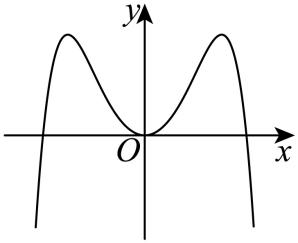
\includegraphics[width=.42\linewidth]{assets/asset-286-01.jpg}
\end{center}
\begin{choices}
  \item A
  \item B
  \item C
  \item D
\end{choices}
\begin{solution}
\textbf{答案：}B

\textbf{分析：}利用函数的奇偶性可排除 A、C，代入 $x=1$ 可得 $f(1)>0$，可排除 D。

\textbf{详解：}$f(-x)=-(-x)^2+(e^{-x}-e^x)\sin(-x)=-x^2+(e^x-e^{-x})\sin x=f(x)$，又函数定义域为 $[-2.8,2.8]$，故该函数为偶函数，可排除 A、C，又 $f(1)=-1+\left(e-\frac{1}{e}\right)\sin1>-1+\left(e-\frac{1}{e}\right)\sin\frac{\pi}{6}=\frac{e}{2}-1-\frac{1}{2e}>\frac{1}{4}-\frac{1}{2e}>0$，故可排除 D。
\end{solution}
\end{question}

\begin{question}[points=5]
\textbf{来源：}2024 年 全国甲卷-理科，第 8 题\quad \textbf{专题：}三角函数\par
已知 $\dfrac{\cos\alpha}{\cos\alpha-\sin\alpha}=3$，则 $\tan\left(\alpha+\dfrac{\pi}{4}\right)=$ （   ）
\begin{choices}
  \item $2\sqrt{3}+1$
  \item $2\sqrt{3}-1$
  \item $\dfrac{3}{2}$
  \item $1-\sqrt{3}$
\end{choices}
\begin{solution}
\textbf{答案：}B

\textbf{分析：}先将 $\dfrac{\cos\alpha}{\cos\alpha-\sin\alpha}$ 弦化切求得 $\tan\alpha$，再根据两角和的正切公式即可求解。

\textbf{详解：}因为 $\dfrac{\cos\alpha}{\cos\alpha-\sin\alpha}=3$，所以 $\dfrac{1}{1-\tan\alpha}=3$，$\Rightarrow\tan\alpha=1-\frac{1}{3}$，所以 $\tan\left(\alpha+\frac{\pi}{4}\right)=\frac{\tan\alpha+1}{1-\tan\alpha}=2\sqrt{3}-1$。
\end{solution}
\end{question}

\begin{question}[points=5]
\textbf{来源：}2024 年 全国甲卷-理科，第 9 题\quad \textbf{专题：}向量\par
已知向量 $\vec{a}=(x+1,x),\vec{b}=(x,2)$，则（   ）
\begin{choices}
  \item “$x=-3$”是“$\vec{a}\perp\vec{b}$”的必要条件
  \item “$x=-3$”是“$\vec{a}\parallel\vec{b}$”的必要条件
  \item “$x=0$”是“$\vec{a}\perp\vec{b}$”的充分条件
  \item “$x=-1+\sqrt{3}$”是“$\vec{a}\parallel\vec{b}$”的充分条件
\end{choices}
\begin{solution}
\textbf{答案：}C

\textbf{分析：}根据向量垂直和平行的坐标表示即可得到方程，解出即可。

\textbf{详解：}对 A，当 $\vec{a}\perp\vec{b}$ 时，则 $\vec{a}\cdot\vec{b}=0$，所以 $x\cdot(x+1)+2x=0$，解得 $x=0$ 或 $-3$，即必要性不成立，故 A 错误；对 C，当 $x=0$ 时，$\vec{a}=(1,0),\vec{b}=(0,2)$，故 $\vec{a}\cdot\vec{b}=0$，所以 $\vec{a}\perp\vec{b}$，即充分性成立，故 C 正确；对 B，当 $\vec{a}\parallel\vec{b}$ 时，则 $2(x+1)=x^2$，解得 $x=1\pm\sqrt{3}$，即必要性不成立，故 B 错误；对 D，当 $x=-1+\sqrt{3}$ 时，不满足 $2(x+1)=x^2$，所以 $\vec{a}\parallel\vec{b}$ 不成立，即充分性不立，故 D 错误。
\end{solution}
\end{question}

\begin{question}[points=5]
\textbf{来源：}2024 年 全国甲卷-理科，第 11 题\quad \textbf{专题：}三角形、三角函数\par
在 $\triangle ABC$ 中内角 $A,B,C$ 所对边分别为 $a,b,c$，若 $B=\dfrac{\pi}{3}$，$b^2=\dfrac{9}{4}ac$，则 $\sin A+\sin C=$ （   ）
\begin{choices}
  \item $\dfrac{3}{2}$
  \item $\sqrt{2}$
  \item $\dfrac{\sqrt{7}}{2}$
  \item $\dfrac{3}{\sqrt{2}}$
\end{choices}
\begin{solution}
\textbf{答案：}C

\textbf{分析：}利用正弦定理得 $\sin A\sin C=\frac{1}{3}$，再利用余弦定理有 $a^2+c^2=\frac{13}{4}ac$，再利用正弦定理得到 $\sin^2 A+\sin^2 C$ 的值，最后代入计算即可。

\textbf{详解：}因为 $B=\frac{\pi}{3},b^2=\frac{9}{4}ac$，则由正弦定理得 $\sin A\sin C=\frac{4}{9}\sin^2 B=\frac{1}{3}$。由余弦定理可得 $b^2=a^2+c^2-ac=\frac{9}{4}ac$，即 $a^2+c^2=\frac{13}{4}ac$，根据正弦定理得 $\sin^2 A+\sin^2 C=\frac{13}{4}\sin A\sin C=\frac{13}{12}$，所以 $(\sin A+\sin C)^2=\sin^2 A+\sin^2 C+2\sin A\sin C=\frac{7}{4}$，因为 $A,C$ 为三角形内角，则 $\sin A+\sin C>0$，则 $\sin A+\sin C=\frac{\sqrt{7}}{2}$。
\end{solution}
\end{question}

\begin{question}[points=5]
\textbf{来源：}2024 年 全国甲卷-文科，第 8 题\quad \textbf{专题：}三角函数\par
函数 $f(x) = -x^2 + (e^x - e^{-x})\sin x$ 在区间 $[-2.8, 2.8]$ 的大致图像为（ ）

\begin{center}
  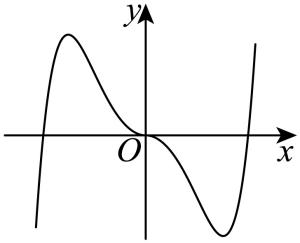
\includegraphics[width=.42\linewidth]{assets/asset-290-01.jpg}
\end{center}
\begin{choices}
  \item A
  \item B
  \item C
  \item D
\end{choices}
\begin{solution}
\textbf{答案：}B

\textbf{分析：}利用函数的奇偶性可排除A、C，代入 $x=1$ 可得 $f(1)>0$，可排除D.

\textbf{详解：}$f(-x) = -(-x)^2 + (e^{-x} - e^x)\sin(-x) = -x^2 + (e^x - e^{-x})\sin x = f(x)$，又函数定义域为 $[-2.8, 2.8]$，故该函数为偶函数，可排除A、C，又 $f(1) = -1 + (e - \frac{1}{e})\sin 1 > -1 + (e - \frac{1}{e})\sin \frac{\pi}{6} = -1 + \frac{e - 1/e}{2} > -\frac{1}{4} + \frac{1}{2e} > 0$，故可排除D.
\end{solution}
\end{question}

\begin{question}[points=5]
\textbf{来源：}2024 年 全国甲卷-文科，第 9 题\quad \textbf{专题：}三角函数\par
已知 $\frac{\cos\alpha}{\cos\alpha - \sin\alpha} = 3$，则 $\tan\left(\alpha + \frac{\pi}{4}\right) =$（ ）
\begin{choices}
  \item $2\sqrt{3} + 1$
  \item $2\sqrt{3} - 1$
  \item $\frac{\sqrt{3}}{2}$
  \item $1 - \sqrt{3}$
\end{choices}
\begin{solution}
\textbf{答案：}B

\textbf{分析：}先将 $\frac{\cos\alpha}{\cos\alpha - \sin\alpha}$ 弦化切求得 $\tan\alpha$，再根据两角和的正切公式即可求解.

\textbf{详解：}因为 $\frac{\cos\alpha}{\cos\alpha - \sin\alpha} = \sqrt{3}$（原卷可能为 $\sqrt{3}$，但文本层显示为3，解析版中也处理为 $\sqrt{3}$），所以 $\frac{1}{1 - \tan\alpha} = \sqrt{3}$，$\Rightarrow \tan\alpha = 1 - \frac{1}{\sqrt{3}} = \frac{\sqrt{3} - 1}{\sqrt{3}}$，所以 $\tan\left(\alpha + \frac{\pi}{4}\right) = \frac{\tan\alpha + 1}{1 - \tan\alpha} = \frac{\frac{\sqrt{3} - 1}{\sqrt{3}} + 1}{1 - \frac{\sqrt{3} - 1}{\sqrt{3}}} = \frac{\frac{2\sqrt{3} - 1}{\sqrt{3}}}{\frac{1}{\sqrt{3}}} = 2\sqrt{3} - 1$.
\end{solution}
\end{question}

\begin{question}[points=5]
\textbf{来源：}2024 年 全国甲卷-文科，第 11 题\quad \textbf{专题：}三角形、三角函数\par
在 $\triangle ABC$ 中，内角 $A, B, C$ 所对边分别为 $a, b, c$，若 $B = \frac{\pi}{3}$，$b^2 = \frac{9}{4}ac$，则 $\sin A + \sin C =$（ ）
\begin{choices}
  \item $\frac{3}{2}$
  \item $\sqrt{2}$
  \item $\frac{\sqrt{7}}{2}$
  \item $\frac{3}{2}$
\end{choices}
\begin{solution}
\textbf{答案：}C

\textbf{分析：}利用正弦定理得 $\sin A \sin C = \frac{1}{3}$，再利用余弦定理有 $a^2 + c^2 = \frac{13}{4}ac$，再利用正弦定理得到 $\sin^2 A + \sin^2 C$ 的值，最后代入计算即可.

\textbf{详解：}因为 $B = \frac{\pi}{3}$，$b^2 = \frac{9}{4}ac$，则由正弦定理得 $\sin A \sin C = \sin^2 B \cdot \frac{4}{9} = \left(\frac{\sqrt{3}}{2}\right)^2 \cdot \frac{4}{9} = \frac{1}{3}$．由余弦定理可得：$b^2 = a^2 + c^2 - ac = \frac{9}{4}ac$，即 $a^2 + c^2 = \frac{13}{4}ac$，根据正弦定理得 $\sin^2 A + \sin^2 C = \frac{13}{4} \sin A \sin C = \frac{13}{4} \times \frac{1}{3} = \frac{13}{12}$，所以 $(\sin A + \sin C)^2 = \sin^2 A + \sin^2 C + 2\sin A \sin C = \frac{13}{12} + \frac{2}{3} = \frac{21}{12} = \frac{7}{4}$，因为 $A, C$ 为三角形内角，则 $\sin A + \sin C > 0$，则 $\sin A + \sin C = \frac{\sqrt{7}}{2}$.
\end{solution}
\end{question}

\begin{question}[points=5]
\textbf{来源：}2024 年 全国甲卷-文科，第 12 题\quad \textbf{专题：}三角函数\par
函数 $f(x) = \sin x - \sqrt{3} \cos x$ 在 $[0, \pi]$ 上的最大值是．
\fillin[{$2$}]
\begin{solution}
\textbf{答案：}$2$

\textbf{分析：}结合辅助角公式化简成正弦型函数，再求给定区间最值即可.

\textbf{详解：}$f(x) = \sin x - \sqrt{3} \cos x = 2\sin\left(x - \frac{\pi}{3}\right)$，当 $x \in [0, \pi]$ 时，$x - \frac{\pi}{3} \in [-\frac{\pi}{3}, \frac{2\pi}{3}]$，当 $x - \frac{\pi}{3} = \frac{\pi}{2}$ 即 $x = \frac{5\pi}{6}$ 时，$f(x)_{\max} = 2$.
\end{solution}
\end{question}

\begin{question}[points=4]
\textbf{来源：}2024 年 上海卷，第 5 题\quad \textbf{专题：}向量\par
已知$k\in\mathbb{R}$，$\vec{a}=(2,5)$，$\vec{b}=(6,k)$，且$\vec{a}\parallel\vec{b}$，则$k$的值为.
\fillin[{$15$}]
\begin{solution}
\textbf{答案：}$15$

\textbf{分析：}根据向量平行的坐标表示得到方程，解出即可.

\textbf{详解：}$\because\vec{a}\parallel\vec{b}$，$\therefore 2k=5\times6$，解得$k=15$．故答案为：15.
\end{solution}
\end{question}

\begin{question}[points=4]
\textbf{来源：}2024 年 上海卷，第 14 题\quad \textbf{专题：}三角函数\par
下列函数$f(x)$的最小正周期是$2\pi$的是（\quad\quad）
\begin{choices}
  \item $A\ \sin x+\cos x$
  \item $B\ \sin x\cos x$
  \item $C\ \sin^2x+\cos^2x$
  \item $D\ \sin^2x-\cos^2x$
\end{choices}
\begin{solution}
\textbf{答案：}$A$

\textbf{分析：}根据辅助角公式、二倍角公式以及同角三角函数关系并结合三角函数的性质一一判断即可.

\textbf{详解：}对A，$\sin x+\cos x=\sqrt{2}\sin\left(x+\frac{\pi}{4}\right)$，周期$T=2\pi$，故A正确；对B，$\sin x\cos x=\frac{1}{2}\sin2x$，周期$T=\frac{2\pi}{2}=\pi$，故B错误；对于选项C，$\sin^2x+\cos^2x=1$，是常值函数，不存在最小正周期，故C错误；对于选项D，$\sin^2x-\cos^2x=-\cos2x$，周期$T=\frac{2\pi}{2}=\pi$，故D错误，故选：A.
\end{solution}
\end{question}

\begin{question}[points=5]
\textbf{来源：}2024 年 上海卷，第 15 题\quad \textbf{专题：}向量\par
定义一个集合$\Omega$，集合中的元素是空间内的点集，任取$P_1,P_2,P_3\in\Omega$，存在不全为0的实数$\lambda_1,\lambda_2,\lambda_3$，使得$\lambda_1\overrightarrow{OP_1}+\lambda_2\overrightarrow{OP_2}+\lambda_3\overrightarrow{OP_3}=\vec{0}$．已知$(1,0,0)\in\Omega$，则$(0,0,1)\notin\Omega$的充分条件是（\quad\quad）
\begin{choices}
  \item $A\ (0,0,0)\in\Omega$
  \item $B\ (-1,0,0)\in\Omega$
  \item $C\ (0,1,0)\in\Omega$
  \item $D\ (0,0,-1)\in\Omega$
\end{choices}
\begin{solution}
\textbf{答案：}$C$

\textbf{分析：}首先分析出三个向量共面，显然当$(1,0,0),(0,0,1),(0,1,0)\in\Omega$时，三个向量构成空间的一个基底，则即可分析出正确答案.

\textbf{详解：}由题意知这三个向量$\overrightarrow{OP_1},\overrightarrow{OP_2},\overrightarrow{OP_3}$共面，即这三个向量不能构成空间的一个基底，对A，由空间直角坐标系易知$(0,0,0),(1,0,0),(0,0,1)$三个向量共面，则当$(-1,0,0),(1,0,0)\in\Omega$无法推出$(0,0,1)\notin\Omega$，故A错误；对B，由空间直角坐标系易知$(-1,0,0),(1,0,0),(0,0,1)$三个向量共面，则当$(0,0,0),(1,0,0)\in\Omega$无法推出$(0,0,1)\notin\Omega$，故A错误；对C，由空间直角坐标系易知$(1,0,0),(0,0,1),(0,1,0)$三个向量不共面，可构成空间的一个基底，则由$(1,0,0),(0,1,0)\in\Omega$能推出$(0,0,1)\notin\Omega$，对D，由空间直角坐标系易知$(1,0,0),(0,0,1),(0,0,-1)$三个向量共面，则当$(0,0,-1)(1,0,0)\in\Omega$无法推出$(0,0,1)\notin\Omega$，故D错误.故选：C.
\end{solution}
\end{question}

\begin{question}[points=18]
\textbf{来源：}2024 年 上海卷，第 20 题\quad \textbf{专题：}向量\par
已知双曲线$\Gamma:x^2-\frac{y^2}{b^2}=1$，$(b>0)$，左右顶点分别为$A_1$，$A_2$，过点$M(-2,0)$的直线$l$交双曲线$\Gamma$于$P$，$Q$两点.（1）若离心率$e=2$时，求$b$的值．（2）若$b=\frac{2\sqrt6}{3}$，$\triangle MA_2P$为等腰三角形时，且点$P$在第一象限，求点$P$的坐标．（3）连接$OQ$并延长，交双曲线$\Gamma$于点$R$，若$\overrightarrow{A_1R}\cdot\overrightarrow{A_2P}=1$，求$b$的取值范围．
\begin{solution}
\textbf{答案：}（1）$b=\sqrt3$；（2）$P(2,2\sqrt2)$；（3）$(0,\sqrt3)\cup(\sqrt3,\frac{\sqrt{30}}{3}]$

\textbf{分析：}（1）根据离心率公式计算即可；（2）分三角形三边分别为底讨论即可；（3）设直线$l:x=my-2$，联立双曲线方程得到韦达定理式，再代入计算向量数量积的等式计算即可.

\textbf{详解：}（1）由题意得$e=\frac{c}{a}=c=2$，则$c=2$，$b=\sqrt{2^2-1}=\sqrt3$．（2）当$b=\frac{2\sqrt6}{3}$时，双曲线$\Gamma:x^2-\frac{y^2}{\frac{8}{3}}=1$，其中$M(-2,0)$，$A_2(1,0)$，因为$\triangle MA_2P$为等腰三角形，则①当以$MA_2$为底时，显然点$P$在直线$x=-\frac12$上，这与点$P$在第一象限矛盾，故舍去；②当以$A_2P$为底时，$MP=MA_2=3$，设$P(x,y)$，则$\begin{cases} x^2-\frac{3y^2}{8}=1 \\ (x+2)^2+y^2=9 \end{cases}$，联立解得$\begin{cases} x=-\frac{23}{11} \\ y=-\frac{8\sqrt{17}}{11} \end{cases}$或$\begin{cases} x=-\frac{23}{11} \\ y=\frac{8\sqrt{17}}{11} \end{cases}$或$\begin{cases} x=1 \\ y=0 \end{cases}$，因为点$P$在第一象限，显然以上均不合题意，舍去；（或者由双曲线性质知$MP>MA_2$，矛盾，舍去）；③当以$MP$为底时，$A_2P=MA_2=3$，设$P(x_0,y_0)$，其中$x_0>0,y_0>0$，则有$\begin{cases} (x_0-1)^2+y_0^2=9 \\ x_0^2-\frac{3y_0^2}{8}=1 \end{cases}$，解得$\begin{cases} x_0=2 \\ y_0=2\sqrt2 \end{cases}$，即$P(2,2\sqrt2)$．综上所述：$P(2,2\sqrt2)$.（3）由题知$A_1(-1,0)$，$A_2(1,0)$，当直线$l$的斜率为0时，此时$\overrightarrow{A_1R}\cdot\overrightarrow{A_2P}=0$，不合题意，则$k_l\neq0$，则设直线$l:x=my-2$，设点$P(x_1,y_1)$，$Q(x_2,y_2)$，根据$OQ$延长线交双曲线$\Gamma$于点$R$，根据双曲线对称性知$R(-x_2,-y_2)$，联立有$\begin{cases} x=my-2 \\ x^2-\frac{y^2}{b^2}=1 \end{cases}\Rightarrow (b^2m^2-1)y^2-4b^2my+3b^2=0$，显然二次项系数$b^2m^2-1\neq0$，其中$\Delta=(-4mb^2)^2-4(b^2m^2-1)3b^2=4b^4m^2+12b^2>0$，$y_1+y_2=\frac{4b^2m}{b^2m^2-1}①$，$y_1y_2=\frac{3b^2}{b^2m^2-1}②$，$\overrightarrow{A_1R}=(-x_2+1,-y_2)$，$\overrightarrow{A_2P}=(x_1-1,y_1)$，则$\overrightarrow{A_1R}\cdot\overrightarrow{A_2P}=(-x_2+1)(x_1-1)-y_1y_2=1$，因为$P(x_1,y_1)$，$Q(x_2,y_2)$在直线$l$上，则$x_1=my_1-2$，$x_2=my_2-2$，即$-(my_2-3)(my_1-3)-y_1y_2=1$，即$y_1y_2(m^2+1)-3m(y_1+y_2)+10=0$，将①②代入有$(m^2+1)\frac{3b^2}{b^2m^2-1}-3m\frac{4b^2m}{b^2m^2-1}+10=0$，即$3b^2(m^2+1)-12b^2m^2+10(b^2m^2-1)=0$，化简得$b^2m^2+3b^2-10=0$，所以$m^2=\frac{10}{b^2}-3$，代入到$b^2m^2-1\neq0$，得$b^2(\frac{10}{b^2}-3)-1=10-3b^2-1=9-3b^2\neq0$，所以$b^2\neq3$，且$m^2=\frac{10}{b^2}-3\ge0$，解得$b^2\le\frac{10}{3}$，又因为$b>0$，则$0<b\le\frac{\sqrt{30}}{3}$，综上知，$b\in(0,\sqrt3)\cup(\sqrt3,\frac{\sqrt{30}}{3}]$.
\end{solution}
\end{question}

\begin{question}[points=5]
\textbf{来源：}2024 年 天津卷，第 4 题\quad \textbf{专题：}三角函数\par
下列函数是偶函数的是 ( )
\begin{choices}
  \item $y = \frac{e^x - x^2}{x^2 + 1}$
  \item $y = \frac{\cos x + x^2}{x^2 + 1}$
  \item $y = \frac{e^x - x}{x + 1}$
  \item $y = \frac{\sin x + 4x}{e^{|x|}}$
\end{choices}
\begin{solution}
\textbf{答案：}$y = \frac{\cos x + x^2}{x^2 + 1}$

\textbf{分析：}根据偶函数的判定方法一一判断即可.

\textbf{详解：}对 A, 设 $f(x)=\frac{e^x-x^2}{x^2+1}$, 定义域为 $\mathbb{R}$, 但 $f(-1)=\frac{e^{-1}-1}{2}$, $f(1)=\frac{e-1}{2}$, 则 $f(-1)\neq f(1)$, 故 A 错误. 对 B, 设 $g(x)=\frac{\cos x+x^2}{x^2+1}$, 定义域为 $\mathbb{R}$, 且 $g(-x)=\frac{\cos(-x)+(-x)^2}{(-x)^2+1}=\frac{\cos x+x^2}{x^2+1}=g(x)$, 则 $g(x)$ 为偶函数, 故 B 正确. 对 C, 设 $h(x)=\frac{e^x-x}{x+1}$, 定义域为 $\{x|x\neq -1\}$, 不关于原点对称, 则 $h(x)$ 不是偶函数, 故 C 错误. 对 D, 设 $\varphi(x)=\frac{\sin x+4x}{e^{|x|}}$, 定义域为 $\mathbb{R}$, 因为 $\varphi(1)=\frac{\sin 1+4}{e}$, $\varphi(-1)=\frac{-\sin 1-4}{e}$, 则 $\varphi(1)\neq\varphi(-1)$, 则 $\varphi(x)$ 不是偶函数, 故 D 错误. 故选 B.
\end{solution}
\end{question}

\begin{question}[points=5]
\textbf{来源：}2024 年 天津卷，第 7 题\quad \textbf{专题：}三角函数\par
已知函数 $f(x)=\sin^3\left(\omega x + \frac{\pi}{3}\right) (\omega>0)$ 的最小正周期为 $\pi$. 则函数在 $\left[-\frac{\pi}{12},\frac{\pi}{6}\right]$ 的最小值是 ( )
\begin{choices}
  \item $-\frac{\sqrt{3}}{2}$
  \item $-\frac{3}{2}$
  \item $0$
  \item $\frac{\sqrt{3}}{2}$
\end{choices}
\begin{solution}
\textbf{答案：}$-\frac{\sqrt{3}}{2}$

\textbf{分析：}先由诱导公式化简, 结合周期公式求出 $\omega$, 得 $f(x)=-\sin 2x$, 再整体求出 $x\in\left[-\frac{\pi}{12},\frac{\pi}{6}\right]$ 时 $2x$ 的范围, 结合正弦三角函数图象特征即可求解.

\textbf{详解：}$f(x)=\sin^3\left(\omega x+\frac{\pi}{3}\right)=\sin(3\omega x+\pi)=-\sin 3\omega x$, 由 $T=\frac{2\pi}{3\omega}=\pi$ 得 $\omega=\frac{2}{3}$, 即 $f(x)=-\sin 2x$. 当 $x\in\left[-\frac{\pi}{12},\frac{\pi}{6}\right]$ 时, $2x\in\left[-\frac{\pi}{6},\frac{\pi}{3}\right]$, 画出 $f(x)=-\sin 2x$ 图象, 由图可知 $f(x)=-\sin 2x$ 在 $\left[-\frac{\pi}{12},\frac{\pi}{6}\right]$ 上递减, 所以当 $x=\frac{\pi}{6}$ 时, $f(x)_{\min}=-\sin\frac{\pi}{3}=-\frac{\sqrt{3}}{2}$. 故选A.
\end{solution}
\end{question}

\begin{question}[points=5]
\textbf{来源：}2024 年 天津卷，第 14 题\quad \textbf{专题：}向量\par
在边长为 $1$ 的正方形 $ABCD$ 中, 点 $E$ 为线段 $CD$ 的三等分点, $CE = \frac{1}{2}DE$, $\overrightarrow{BE} = \lambda \overrightarrow{BA} + \mu \overrightarrow{BC}$, 则 $\lambda+\mu =$ ; 若 $F$ 为线段 $BE$ 上的动点, $G$ 为 $AF$ 中点, 则 $\overrightarrow{AF} \cdot \overrightarrow{DG}$ 的最小值为.
\fillin[{$\frac{4}{3}$, $-\frac{5}{18}$}]
\begin{solution}
\textbf{答案：}$\frac{4}{3}$, $-\frac{5}{18}$

\textbf{分析：}解法一: 以 $\overrightarrow{BA},\overrightarrow{BC}$ 为基底, 根据向量的线性运算求 $\overrightarrow{BE}$, 可得 $\lambda+\mu$, 设 $\overrightarrow{BF}=k\overrightarrow{BE}$, 求 $\overrightarrow{AF},\overrightarrow{DG}$, 结合数量积的运算律求最小值. 解法二: 建系标点, 根据向量的坐标运算求 $\overrightarrow{BE}$, 可得 $\lambda+\mu$, 设 $F(a,-3a),a\in[-\frac{1}{3},0]$, 求 $\overrightarrow{AF},\overrightarrow{DG}$, 结合数量积的坐标运算求最小值.

\textbf{详解：}解法一: 因为 $CE=\frac{1}{2}DE$, 即 $\overrightarrow{CE}=\frac{1}{3}\overrightarrow{BA}$, 则 $\overrightarrow{BE}=\overrightarrow{BC}+\overrightarrow{CE}=\frac{1}{3}\overrightarrow{BA}+\overrightarrow{BC}$, 所以 $\lambda=\frac{1}{3},\mu=1$, $\lambda+\mu=\frac{4}{3}$. 由题意 $|\overrightarrow{BC}|=|\overrightarrow{BA}|=1$, $\overrightarrow{BA}\cdot\overrightarrow{BC}=0$. 设 $\overrightarrow{BF}=k\overrightarrow{BE}= \frac{k}{3}\overrightarrow{BA}+k\overrightarrow{BC}$, $k\in[0,1]$. 则 $\overrightarrow{AF}=\overrightarrow{AB}+\overrightarrow{BF}=(\frac{k}{3}-1)\overrightarrow{BA}+k\overrightarrow{BC}$. 又 $G$ 为 $AF$ 中点, $\overrightarrow{DG}=\overrightarrow{DA}+\overrightarrow{AG}=-\overrightarrow{BC}+\frac{1}{2}\overrightarrow{AF}=\frac{1}{2}(\frac{k}{3}-1)\overrightarrow{BA}+(\frac{k}{2}-1)\overrightarrow{BC}$. 则 $\overrightarrow{AF}\cdot\overrightarrow{DG}=[ (\frac{k}{3}-1)\overrightarrow{BA}+k\overrightarrow{BC} ]\cdot[\frac{1}{2}(\frac{k}{3}-1)\overrightarrow{BA}+(\frac{k}{2}-1)\overrightarrow{BC}] =\frac{1}{2}(\frac{k}{3}-1)^2 + k(\frac{k}{2}-1)=\frac{5}{9}(k-\frac{6}{5})^2-\frac{3}{10}$, 又 $k\in[0,1]$, 当 $k=1$ 时取最小值 $-\frac{5}{18}$.
\end{solution}
\end{question}

\begin{question}[points=14]
\textbf{来源：}2024 年 天津卷，第 16 题\quad \textbf{专题：}三角形、三角函数\par
在 $\triangle ABC$ 中, $\cos B = \frac{9}{16}$, $b=5$, $\frac{a}{c}=\frac{2}{3}$.

(1) 求 $a$;

(2) 求 $\sin A$;

(3) 求 $\cos(B-2A)$.
\begin{solution}
\textbf{答案：}(1) $a=4$; (2) $\sin A = \frac{\sqrt{7}}{4}$; (3) $\frac{57}{64}$

\textbf{分析：}(1) 设 $a=2t,c=3t$, 利用余弦定理即可得到方程, 解出即可. (2) 法一: 求出 $\sin B$, 再利用正弦定理; 法二: 利用余弦定理求出 $\cos A$, 则得到 $\sin A$. (3) 法一: 根据大边对大角确定 $A$ 为锐角, 则得到 $\cos A$, 再利用二倍角公式和两角差的余弦公式即可. 法二: 直接利用二倍角公式和两角差的余弦公式即可.

\textbf{详解：}(1) 设 $a=2t$, $c=3t$, $t>0$, 则根据余弦定理得 $b^2=a^2+c^2-2ac\cos B$, 即 $25=4t^2+9t^2-2\times2t\times3t\times\frac{9}{16}$, 解得 $t=2$ (负舍), 则 $a=4$, $c=6$.
(2) 法一: 因为 $B$ 为三角形内角, 所以 $\sin B = \sqrt{1-\cos^2 B} = \sqrt{1-\left(\frac{9}{16}\right)^2} = \frac{5\sqrt{7}}{16}$, 再根据正弦定理 $\frac{a}{\sin A}=\frac{b}{\sin B}$, 即 $\frac{4}{\sin A}=\frac{5}{\frac{5\sqrt{7}}{16}}$, 解得 $\sin A = \frac{\sqrt{7}}{4}$.
(3) 法一: 因为 $\cos B=\frac{9}{16}>0$, 且 $B\in(0,\pi)$, 所以 $B\in(0,\frac{\pi}{2})$. 由(2)法一知 $\sin B=\frac{5\sqrt{7}}{16}$. 因为 $a<b$, 则 $A<B$, 所以 $\cos A=\sqrt{1-\sin^2 A}=\sqrt{1-\left(\frac{\sqrt{7}}{4}\right)^2}=\frac{3}{4}$. 则 $\sin2A=2\sin A\cos A=2\times\frac{\sqrt{7}}{4}\times\frac{3}{4}=\frac{3\sqrt{7}}{8}$, $\cos2A=2\cos^2 A-1=2\times\left(\frac{3}{4}\right)^2-1=\frac{1}{8}$. $\cos(B-2A)=\cos B\cos2A+\sin B\sin2A=\frac{9}{16}\times\frac{1}{8}+\frac{5\sqrt{7}}{16}\times\frac{3\sqrt{7}}{8}=\frac{9}{128}+\frac{105}{128}=\frac{114}{128}=\frac{57}{64}$.
\end{solution}
\end{question}

\begin{question}[points=15]
\textbf{来源：}2024 年 天津卷，第 18 题\quad \textbf{专题：}向量\par
已知椭圆 $\frac{x^2}{a^2}+\frac{y^2}{b^2}=1(a>b>0)$ 的离心率 $e=\frac{1}{2}$. 左顶点为 $A$, 下顶点为 $B$, $C$ 是线段 $OB$ 的中点, 其中 $S_{\triangle ABC}=\frac{3\sqrt{3}}{2}$.

(1) 求椭圆方程.

(2) 过点 $(0,-\frac{3}{2})$ 的动直线与椭圆有两个交点 $P$, $Q$. 在 $y$ 轴上是否存在点 $T$ 使得 $\overrightarrow{TP}\cdot\overrightarrow{TQ}\leq 0$ 恒成立. 若存在求出这个 $T$ 点纵坐标的取值范围, 若不存在请说明理由.
\begin{solution}
\textbf{答案：}(1) $\frac{x^2}{12}+\frac{y^2}{9}=1$; (2) 存在 $T(0,t)$ 且 $-3\leq t\leq \frac{3}{2}$, 使得 $\overrightarrow{TP}\cdot\overrightarrow{TQ}\leq 0$ 恒成立.

\textbf{分析：}(1) 根据椭圆的离心率和三角形的面积可求基本量, 从而可得椭圆的标准方程. (2) 设直线方程, 与椭圆联立, 利用韦达定理和向量数量积的坐标运算, 结合恒成立条件求 $t$ 的范围.

\textbf{详解：}(1) 因为 $e=\frac{1}{2}$, 故 $a=2c$, $b=\sqrt{3}c$. 所以 $A(-2c,0)$, $B(0,-\sqrt{3}c)$, $C(0,-\frac{\sqrt{3}}{2}c)$. $S_{\triangle ABC}=\frac{1}{2}\times 2c\times \frac{\sqrt{3}}{2}c=\frac{\sqrt{3}}{2}c^2=\frac{3\sqrt{3}}{2}$, 解得 $c=\sqrt{3}$, 所以 $a=2\sqrt{3}$, $b=3$, 故椭圆方程为 $\frac{x^2}{12}+\frac{y^2}{9}=1$.
(2) 设过点 $(0,-\frac{3}{2})$ 的动直线方程为 $y=kx-\frac{3}{2}$, $P(x_1,y_1)$, $Q(x_2,y_2)$, $T(0,t)$. 联立 $\begin{cases} 3x^2+4y^2=36 \\ y=kx-\frac{3}{2} \end{cases}$, 得 $(3+4k^2)x^2-12kx-27=0$, $\Delta>0$, $x_1+x_2=\frac{12k}{3+4k^2}$, $x_1x_2=-\frac{27}{3+4k^2}$. $\overrightarrow{TP}=(x_1,y_1-t)$, $\overrightarrow{TQ}=(x_2,y_2-t)$. $\overrightarrow{TP}\cdot\overrightarrow{TQ}=x_1x_2+(y_1-t)(y_2-t)=x_1x_2+(kx_1-\frac{3}{2}-t)(kx_2-\frac{3}{2}-t)=(1+k^2)x_1x_2-k(\frac{3}{2}+t)(x_1+x_2)+(\frac{3}{2}+t)^2$. 代入韦达定理, 得 $\frac{[(3+2t)^2-12t-45]k^2+3(\frac{3}{2}+t)^2-27}{3+4k^2}$. 要使 $\overrightarrow{TP}\cdot\overrightarrow{TQ}\leq 0$ 恒成立, 需 $\begin{cases} (3+2t)^2-12t-45\leq 0 \\ 3(\frac{3}{2}+t)^2-27\leq 0 \end{cases}$, 解得 $-3\leq t\leq \frac{3}{2}$. 当斜率不存在时, 直线为 $x=0$, 与椭圆交于 $(0,3)$, $(0,-3)$, 此时需 $-3\leq t\leq 3$, 结合得 $-3\leq t\leq \frac{3}{2}$. 综上, 存在 $T(0,t)$ 且 $-3\leq t\leq \frac{3}{2}$, 使得 $\overrightarrow{TP}\cdot\overrightarrow{TQ}\leq 0$ 恒成立.
\end{solution}
\end{question}

\begin{question}[points=5]
\textbf{来源：}2024 年 新高考II卷，第 3 题\quad \textbf{专题：}向量\par
已知向量$\vec{a}, \vec{b}$满足$|\vec{a}|=1$，$|\vec{a}+2\vec{b}|=2$，且$(\vec{b}-2\vec{a}) \perp \vec{b}$，则$|\vec{b}|=$（ ）
\begin{choices}
  \item $\dfrac{1}{2}$
  \item $\dfrac{\sqrt{2}}{2}$
  \item $\dfrac{\sqrt{3}}{2}$
  \item $1$
\end{choices}
\begin{solution}
\textbf{答案：}$B$

\textbf{分析：}由$(\vec{b}-2\vec{a})\perp\vec{b}$得$|\vec{b}|^2=2\vec{a}\cdot\vec{b}$，结合$|\vec{a}|=1$，$|\vec{a}+2\vec{b}|=2$，得$1+4\vec{a}\cdot\vec{b}+4|\vec{b}|^2=1+6|\vec{b}|^2=4$，由此即可得解.

\textbf{详解：}因为$(\vec{b}-2\vec{a})\perp\vec{b}$，所以$(\vec{b}-2\vec{a})\cdot\vec{b}=0$，即$|\vec{b}|^2=2\vec{a}\cdot\vec{b}$。又因为$|\vec{a}|=1$，$|\vec{a}+2\vec{b}|=2$，所以$1+4\vec{a}\cdot\vec{b}+4|\vec{b}|^2=1+6|\vec{b}|^2=4$，从而$|\vec{b}|=\dfrac{\sqrt{2}}{2}$.
\end{solution}
\end{question}

\begin{question}[points=5]
\textbf{来源：}2024 年 新高考II卷，第 6 题\quad \textbf{专题：}三角函数\par
设函数$f(x)=a(x+1)^2-1$，$g(x)=\cos x+2ax$，当$x\in(-1,1)$时，曲线$y=f(x)$与$y=g(x)$恰有一个交点，则$a=$（ ）
\begin{choices}
  \item $-1$
  \item $\dfrac{1}{2}$
  \item $1$
  \item $2$
\end{choices}
\begin{solution}
\textbf{答案：}$D$

\textbf{分析：}解法一：令$F(x)=ax^2+a-1$，$G(x)=\cos x$，分析可知曲线$y=F(x)$与$y=G(x)$恰有一个交点，结合偶函数的对称性可知该交点只能在$y$轴上，即可得$a=2$，并代入检验即可；解法二：令$h(x)=f(x)-g(x),x\in(-1,1)$，可知$h(x)$为偶函数，根据偶函数的对称性可知$h(x)$的零点只能为0，即可得$a=2$，并代入检验即可.

\textbf{详解：}解法一：令$f(x)=g(x)$，即$a(x+1)^2-1=\cos x+2ax$，可得$ax^2+a-1=\cos x$。令$F(x)=ax^2+a-1$，$G(x)=\cos x$。原题意等价于当$x\in(-1,1)$时，曲线$y=F(x)$与$y=G(x)$恰有一个交点。注意到$F(x),G(x)$均为偶函数，可知该交点只能在$y$轴上，可得$F(0)=G(0)$，即$a-1=1$，解得$a=2$。若$a=2$，令$F(x)=G(x)$，可得$2x^2+1-\cos x=0$。因为$x\in(-1,1)$，则$2x^2\ge0$，$1-\cos x\ge0$，当且仅当$x=0$时等号成立，可得$2x^2+1-\cos x\ge0$，当且仅当$x=0$时等号成立，则方程$2x^2+1-\cos x=0$有且仅有一个实根0，即曲线$y=F(x)$与$y=G(x)$恰有一个交点，所以$a=2$符合题意。综上所述：$a=2$。解法二：令$h(x)=f(x)-g(x)=ax^2+a-1-\cos x,x\in(-1,1)$，原题意等价于$h(x)$有且仅有一个零点。因为$h(-x)=a(-x)^2+a-1-\cos(-x)=ax^2+a-1-\cos x=h(x)$，则$h(x)$为偶函数，根据偶函数的对称性可知$h(x)$的零点只能为0，即$h(0)=a-2=0$，解得$a=2$。若$a=2$，则$h(x)=2x^2+1-\cos x,x\in(-1,1)$，又因为$2x^2\ge0$，$1-\cos x\ge0$当且仅当$x=0$时等号成立，可得$h(x)\ge0$，当且仅当$x=0$时等号成立，即$h(x)$有且仅有一个零点0，所以$a=2$符合题意.
\end{solution}
\end{question}

\begin{question}[points=6]
\textbf{来源：}2024 年 新高考II卷，第 9 题\quad \textbf{专题：}三角函数\par
对于函数$f(x)=\sin 2x$和$g(x)=\sin(2x-\dfrac{\pi}{4})$，下列正确的有（ ）
\begin{choices}
  \item $f(x)$与$g(x)$有相同零点
  \item $f(x)$与$g(x)$有相同最大值
  \item $f(x)$与$g(x)$有相同的最小正周期
  \item $f(x)$与$g(x)$的图像有相同的对称轴
\end{choices}
\begin{solution}
\textbf{答案：}$BC$

\textbf{分析：}根据正弦函数的零点、最值、周期公式、对称轴方程逐一分析每个选项即可.

\textbf{详解：}A选项，令$f(x)=\sin 2x=0$，解得$x=\dfrac{k\pi}{2},k\in\mathbb{Z}$，即为$f(x)$零点；令$g(x)=\sin(2x-\dfrac{\pi}{4})=0$，解得$x=\dfrac{k\pi}{2}+\dfrac{\pi}{8},k\in\mathbb{Z}$，即为$g(x)$零点，显然$f(x),g(x)$零点不同，A选项错误。B选项，显然$f(x)_{\max}=g(x)_{\max}=1$，B选项正确。C选项，根据周期公式，$f(x),g(x)$的周期均为$\dfrac{2\pi}{2}=\pi$，C选项正确。D选项，根据正弦函数的性质$f(x)$的对称轴满足$2x=k\pi+\dfrac{\pi}{2}\Leftrightarrow x=\dfrac{k\pi}{2}+\dfrac{\pi}{4},k\in\mathbb{Z}$，$g(x)$的对称轴满足$2x-\dfrac{\pi}{4}=k\pi+\dfrac{\pi}{2}\Leftrightarrow x=\dfrac{k\pi}{2}+\dfrac{3\pi}{8},k\in\mathbb{Z}$，显然$f(x),g(x)$图像的对称轴不同，D选项错误.
\end{solution}
\end{question}

\begin{question}[points=5]
\textbf{来源：}2024 年 新高考II卷，第 13 题\quad \textbf{专题：}三角函数\par
已知$\alpha$为第一象限角，$\beta$为第三象限角，$\tan\alpha+\tan\beta=4$，$\tan\alpha\tan\beta=\sqrt{2}+1$，则$\sin(\alpha+\beta)=$.
\fillin[{$-\dfrac{2\sqrt{2}}{3}$}]
\begin{solution}
\textbf{答案：}$-\dfrac{2\sqrt{2}}{3}$

\textbf{分析：}法一：根据两角和与差的正切公式得$\tan(\alpha+\beta)=-2\sqrt{2}$，再缩小$\alpha+\beta$的范围，最后结合同角的平方和关系即可得到答案；法二：利用弦化切的方法即可得到答案.

\textbf{详解：}法一：由题意得$\tan(\alpha+\beta)=\dfrac{\tan\alpha+\tan\beta}{1-\tan\alpha\tan\beta}=\dfrac{4}{1-(\sqrt{2}+1)}=-2\sqrt{2}$。因为$\alpha\in\left(2k\pi,2k\pi+\dfrac{\pi}{2}\right)$，$\beta\in\left(2m\pi+\pi,2m\pi+\dfrac{3\pi}{2}\right)$，$k,m\in\mathbb{Z}$，则$\alpha+\beta\in( (2m+2k)\pi+\pi, (2m+2k)\pi+2\pi )$，$k,m\in\mathbb{Z}$。又因为$\tan(\alpha+\beta)=-2\sqrt{2}<0$，则$\alpha+\beta\in\left( (2m+2k)\pi+\dfrac{3\pi}{2}, (2m+2k)\pi+2\pi\right)$，$k,m\in\mathbb{Z}$，则$\sin(\alpha+\beta)<0$。由$\dfrac{\sin(\alpha+\beta)}{\cos(\alpha+\beta)}=-2\sqrt{2}$，联立$\sin^2(\alpha+\beta)+\cos^2(\alpha+\beta)=1$，解得$\sin(\alpha+\beta)=-\dfrac{2\sqrt{2}}{3}$。法二：因为$\alpha$为第一象限角，$\beta$为第三象限角，则$\cos\alpha>0$，$\cos\beta<0$。$\cos\alpha=\dfrac{\cos\alpha}{\sin^2\alpha+\cos^2\alpha}=\dfrac{1}{\sqrt{1+\tan^2\alpha}}$，$\cos\beta=\dfrac{\cos\beta}{\sin^2\beta+\cos^2\beta}=\dfrac{-1}{\sqrt{1+\tan^2\beta}}$，则$\sin(\alpha+\beta)=\sin\alpha\cos\beta+\cos\alpha\sin\beta=\cos\alpha\cos\beta(\tan\alpha+\tan\beta)=4\cos\alpha\cos\beta=\dfrac{-4}{\sqrt{1+\tan^2\alpha}\sqrt{1+\tan^2\beta}}=\dfrac{-4}{\sqrt{(\tan\alpha+\tan\beta)^2+(\tan\alpha\tan\beta-1)^2}}=\dfrac{-4}{\sqrt{4^2+(\sqrt{2})^2}}=-\dfrac{2\sqrt{2}}{3}$.
\end{solution}
\end{question}

\begin{question}[points=15]
\textbf{来源：}2024 年 新高考II卷，第 15 题\quad \textbf{专题：}三角形、三角函数\par
记$\triangle ABC$的内角$A,B,C$的对边分别为$a,b,c$，已知$\sin A+\sqrt{3}\cos A=2$.

(1)求$A$.

(2)若$a=2$，$2b\sin C=c\sin 2B$，求$\triangle ABC$的周长.
\begin{solution}
\textbf{答案：}(1)$A=\dfrac{\pi}{6}$
(2)$2+\sqrt{6}+3\sqrt{2}$

\textbf{分析：}(1)根据辅助角公式对条件$\sin A+\sqrt{3}\cos A=2$进行化简处理即可求解，常规方法还可利用同角三角函数的关系解方程组，亦可利用导数、向量数量积公式、万能公式解决；(2)先根据正弦定理边角互化算出$B$，然后根据正弦定理算出$b,c$即可得出周长.

\textbf{详解：}（1）方法一（辅助角公式）：由$\sin A+\sqrt{3}\cos A=2$可得$\dfrac{1}{2}\sin A+\dfrac{\sqrt{3}}{2}\cos A=1$，即$\sin\left(A+\dfrac{\pi}{3}\right)=1$。由于$A\in(0,\pi)\Rightarrow A+\dfrac{\pi}{3}\in\left(\dfrac{\pi}{3},\dfrac{4\pi}{3}\right)$，故$A+\dfrac{\pi}{3}=\dfrac{\pi}{2}$，解得$A=\dfrac{\pi}{6}$。
方法二（同角三角函数的基本关系）：由$\sin A+\sqrt{3}\cos A=2$，又$\sin^2 A+\cos^2 A=1$，消去$\sin A$得到：$4\cos^2 A-4\sqrt{3}\cos A+3=0\Leftrightarrow(2\cos A-\sqrt{3})^2=0$，解得$\cos A=\dfrac{\sqrt{3}}{2}$，又$A\in(0,\pi)$，故$A=\dfrac{\pi}{6}$。
方法三（利用极值点求解）：设$f(x)=\sin x+\sqrt{3}\cos x(0<x<\pi)$，则$f(x)=2\sin\left(x+\dfrac{\pi}{3}\right)(0<x<\pi)$。显然$x=\dfrac{\pi}{6}$时，$f(x)_{\max}=2$。注意到$f(A)=\sin A+\sqrt{3}\cos A=2=2\sin\left(A+\dfrac{\pi}{3}\right)$，$f(x)_{\max}=f(A)$，在开区间$(0,\pi)$上取到最大值，于是$x=A$必定是极值点，即$f'(A)=0=\cos A-\sqrt{3}\sin A$，即$\tan A=\dfrac{\sqrt{3}}{3}$，又$A\in(0,\pi)$，故$A=\dfrac{\pi}{6}$。
方法四（利用向量数量积公式）：设$\vec{a}=(1,\sqrt{3})$，$\vec{b}=(\sin A,\cos A)$，由题意，$\vec{a}\cdot\vec{b}=\sin A+\sqrt{3}\cos A=2$，根据向量的数量积公式，$\vec{a}\cdot\vec{b}=|\vec{a}||\vec{b}|\cos\langle\vec{a},\vec{b}\rangle=2\cos\langle\vec{a},\vec{b}\rangle$，则$2\cos\langle\vec{a},\vec{b}\rangle=2\Leftrightarrow\cos\langle\vec{a},\vec{b}\rangle=1$，此时$\langle\vec{a},\vec{b}\rangle=0$，即$\vec{a},\vec{b}$同向共线。根据向量共线条件，$1\cdot\cos A=\sqrt{3}\cdot\sin A\Leftrightarrow\tan A=\dfrac{\sqrt{3}}{3}$，又$A\in(0,\pi)$，故$A=\dfrac{\pi}{6}$。
方法五（利用万能公式求解）：设$t=\tan\dfrac{A}{2}$，根据万能公式，$\sin A+\sqrt{3}\cos A=2=\dfrac{2t}{1+t^2}+\dfrac{\sqrt{3}(1-t^2)}{1+t^2}$，整理可得$t^2-2(2-\sqrt{3})t+(2-\sqrt{3})^2=0=(t-(2-\sqrt{3}))^2$，解得$\tan\dfrac{A}{2}=t=2-\sqrt{3}$，根据二倍角公式，$\tan A=\dfrac{2t}{1-t^2}=\dfrac{\sqrt{3}}{3}$，又$A\in(0,\pi)$，故$A=\dfrac{\pi}{6}$。
（2）由题设条件和正弦定理$2b\sin C=c\sin2B\Leftrightarrow2\sin B\sin C=2\sin C\sin B\cos B$，又$B,C\in(0,\pi)$，则$\sin B\sin C\neq0$，进而$\cos B=\dfrac{\sqrt{2}}{2}$，得到$B=\dfrac{\pi}{4}$，于是$C=\pi-A-B=\dfrac{7\pi}{12}$，$\sin C=\sin(\pi-A-B)=\sin(A+B)=\sin A\cos B+\sin B\cos A=\dfrac{\sqrt{2}+\sqrt{6}}{4}$。由正弦定理可得$\dfrac{a}{\sin A}=\dfrac{b}{\sin B}=\dfrac{c}{\sin C}$，即$\dfrac{2}{\sin\dfrac{\pi}{6}}=\dfrac{b}{\sin\dfrac{\pi}{4}}=\dfrac{c}{\sin\dfrac{7\pi}{12}}$，解得$b=2\sqrt{2}$，$c=\sqrt{6}+\sqrt{2}$，故$\triangle ABC$的周长为$2+\sqrt{6}+3\sqrt{2}$.
\end{solution}
\end{question}

\begin{question}[points=15]
\textbf{来源：}2024 年 新高考II卷，第 17 题\quad \textbf{专题：}向量\par
如图，平面四边形$ABCD$中，$AB=8$，$CD=3$，$AD=5\sqrt{3}$，$\angle ADC=90^\circ$，$\angle BAD=30^\circ$，点$E,F$满足$\overrightarrow{AE}=\dfrac{2}{5}\overrightarrow{AD}$，$\overrightarrow{AF}=\dfrac{1}{2}\overrightarrow{AB}$，将$\triangle AEF$沿$EF$对折至$\triangle PEF$，使得$PC=4\sqrt{3}$.

(1)证明：$EF\perp PD$；

(2)求面$PCD$与面$PBF$所成的二面角的正弦值.

\begin{center}
  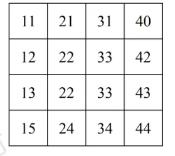
\includegraphics[width=.42\linewidth]{assets/asset-308-01.jpg}
\end{center}

\begin{center}
  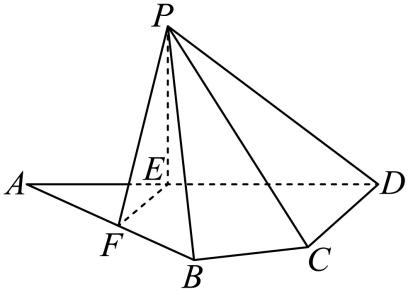
\includegraphics[width=.42\linewidth]{assets/asset-308-02.jpg}
\end{center}
\begin{solution}
\textbf{答案：}(1)证明见解析
(2)$\dfrac{8\sqrt{65}}{65}$

\textbf{分析：}(1)由题意，根据余弦定理求得$EF=2$，利用勾股定理的逆定理可证得$EF\perp AD$，则$EF\perp PE$，$EF\perp DE$，结合线面垂直的判定定理与性质即可证明；(2)由(1)，根据线面垂直的判定定理与性质可证明$PE\perp ED$，建立如图空间直角坐标系$E-xyz$，利用空间向量法求解面面角即可.

\textbf{详解：}（1）由$AB=8,AD=5\sqrt{3},\overrightarrow{AE}=\dfrac{2}{5}\overrightarrow{AD},\overrightarrow{AF}=\dfrac{1}{2}\overrightarrow{AB}$，得$AE=2\sqrt{3},AF=4$。又$\angle BAD=30^\circ$，在$\triangle AEF$中，由余弦定理得$EF=\sqrt{AE^2+AF^2-2AE\cdot AF\cos\angle BAD}=\sqrt{16+12-2\cdot4\cdot2\sqrt{3}\cdot\dfrac{\sqrt{3}}{2}}=2$，所以$AE^2+EF^2=AF^2$，则$AE\perp EF$，即$EF\perp AD$，所以$EF\perp PE$，$EF\perp DE$，又$PE\cap DE=E$，$PE,DE\subset$平面$PDE$，所以$EF\perp$平面$PDE$，又$PD\subset$平面$PDE$，故$EF\perp PD$。
（2）连接$CE$，由$\angle ADC=90^\circ,ED=3\sqrt{3},CD=3$，则$CE^2=ED^2+CD^2=36$。在$\triangle PEC$中，$PC=4\sqrt{3},PE=2\sqrt{3},EC=6$，得$EC^2+PE^2=PC^2$，所以$PE\perp EC$，由(1)知$PE\perp EF$，又$EC\cap EF=E$，$EC,EF\subset$平面$ABCD$，所以$PE\perp$平面$ABCD$，又$ED\subset$平面$ABCD$，所以$PE\perp ED$，则$PE,EF,ED$两两垂直，建立如图空间直角坐标系$E-xyz$，则$E(0,0,0)$，$P(0,0,2\sqrt{3})$，$D(0,3\sqrt{3},0)$，$C(3,3\sqrt{3},0)$，$F(2,0,0)$，$A(0,-2\sqrt{3},0)$，由$F$是$AB$的中点，得$B(4,2\sqrt{3},0)$。所以$\overrightarrow{PC}=(3,3\sqrt{3},-2\sqrt{3})$，$\overrightarrow{PD}=(0,3\sqrt{3},-2\sqrt{3})$，$\overrightarrow{PB}=(4,2\sqrt{3},-2\sqrt{3})$，$\overrightarrow{PF}=(2,0,-2\sqrt{3})$。设平面$PCD$和平面$PBF$的一个法向量分别为$\vec{n}=(x_1,y_1,z_1)$，$\vec{m}=(x_2,y_2,z_2)$，则$\begin{cases}\vec{n}\cdot\overrightarrow{PC}=3x_1+3\sqrt{3}y_1-2\sqrt{3}z_1=0\\\vec{n}\cdot\overrightarrow{PD}=3\sqrt{3}y_1-2\sqrt{3}z_1=0\end{cases}$，$\begin{cases}\vec{m}\cdot\overrightarrow{PB}=4x_2+2\sqrt{3}y_2-2\sqrt{3}z_2=0\\\vec{m}\cdot\overrightarrow{PF}=2x_2-2\sqrt{3}z_2=0\end{cases}$，令$y_1=2$，$x_2=\sqrt{3}$，得$x_1=0,z_1=3,y_2=-1,z_2=1$，所以$\vec{n}=(0,2,3)$，$\vec{m}=(\sqrt{3},-1,1)$，所以$\cos\langle\vec{m},\vec{n}\rangle=\dfrac{\vec{m}\cdot\vec{n}}{|\vec{m}||\vec{n}|}=\dfrac{1}{5\cdot\sqrt{13}}=\dfrac{\sqrt{65}}{65}$。设平面$PCD$和平面$PBF$所成角为$\theta$，则$\sin\theta=\sqrt{1-\cos^2\theta}=\dfrac{8\sqrt{65}}{65}$，即平面$PCD$和平面$PBF$所成角的正弦值为$\dfrac{8\sqrt{65}}{65}$.
\end{solution}
\end{question}

\begin{question}[points=17]
\textbf{来源：}2024 年 新高考II卷，第 19 题\quad \textbf{专题：}向量\par
已知双曲线$C:x^2-y^2=m(m>0)$，点$P_1(5,4)$在$C$上，$k$为常数，$0<k<1$。按照如下方式依次构造点$P_n(n=2,3,\ldots)$，过$P_{n-1}$作斜率为$k$的直线与$C$的左支交于点$Q_{n-1}$，令$P_n$为$Q_{n-1}$关于$y$轴的对称点，记$P_n$的坐标为$(x_n,y_n)$。

(1)若$k=\dfrac{1}{2}$，求$x_2,y_2$；

(2)证明：数列$\{x_n-y_n\}$是公比为$\dfrac{1+k}{1-k}$的等比数列；

(3)设$S_n$为$\triangle P_nP_{n+1}P_{n+2}$的面积，证明：对任意的正整数$n$，$S_n=S_{n+1}$.
\begin{solution}
\textbf{答案：}(1)$x_2=3$，$y_2=0$
(2)证明见解析
(3)证明见解析

\textbf{分析：}(1)直接根据题目中的构造方式计算出$P_2$的坐标即可；(2)根据等比数列的定义即可验证结论；(3)思路一：使用平面向量数量积和等比数列工具，证明$S_n$的取值为与$n$无关的定值即可。思路二：使用等差数列工具，证明$S_n$的取值为与$n$无关的定值即可.

\textbf{详解：}（1）由已知有$m=5^2-4^2=9$，故$C$的方程为$x^2-y^2=9$。当$k=\dfrac{1}{2}$时，过$P_1(5,4)$且斜率为$\dfrac{1}{2}$的直线为$y=\dfrac{x+3}{2}$，与$x^2-y^2=9$联立得到$x^2-\left(\dfrac{x+3}{2}\right)^2=9$，解得$x=-3$或$x=5$，所以该直线与$C$的不同于$P_1$的交点为$Q_1(-3,0)$（在左支上），故$P_2(3,0)$，从而$x_2=3,y_2=0$。
（2）过$P_n(x_n,y_n)$且斜率为$k$的直线为$y=k(x-x_n)+y_n$，与$x^2-y^2=9$联立得$x^2-[k(x-x_n)+y_n]^2=9$，展开得$(1-k^2)x^2-2k(y_n-kx_n)x-[(y_n-kx_n)^2+9]=0$。由于$P_n$是公共点，故方程有一根$x=x_n$。设另一根为$x'$，由韦达定理$x_n+x'=\dfrac{2k(y_n-kx_n)}{1-k^2}$，则$x'=\dfrac{2k(y_n-kx_n)}{1-k^2}-x_n=\dfrac{2ky_n-x_n-k^2x_n}{1-k^2}$，相应的$y'=k(x'-x_n)+y_n=\dfrac{y_n+k^2y_n-2kx_n}{1-k^2}$。所以该直线与$C$的不同于$P_n$的交点为$Q_n\left(\dfrac{2ky_n-x_n-k^2x_n}{1-k^2},\dfrac{y_n+k^2y_n-2kx_n}{1-k^2}\right)$，该点在左支上。$P_{n+1}$为$Q_n$关于$y$轴的对称点，故$x_{n+1}=\dfrac{x_n+k^2x_n-2ky_n}{1-k^2}$，$y_{n+1}=\dfrac{y_n+k^2y_n-2kx_n}{1-k^2}$。所以$x_{n+1}-y_{n+1}=\dfrac{x_n+k^2x_n-2ky_n}{1-k^2}-\dfrac{y_n+k^2y_n-2kx_n}{1-k^2}=\dfrac{1+k^2+2k}{1-k^2}(x_n-y_n)=\dfrac{1+k}{1-k}(x_n-y_n)$。又$x_1-y_1=1\neq0$，所以数列$\{x_n-y_n\}$是公比为$\dfrac{1+k}{1-k}$的等比数列。
（3）由(2)可得$x_{n+1}+y_{n+1}=\dfrac{x_n+k^2x_n-2ky_n}{1-k^2}+\dfrac{y_n+k^2y_n-2kx_n}{1-k^2}=\dfrac{1+k^2-2k}{1-k^2}(x_n+y_n)=\dfrac{1-k}{1+k}(x_n+y_n)$，所以数列$\{x_n+y_n\}$是公比为$\dfrac{1-k}{1+k}$的等比数列。因此，对任意正整数$n$，有$x_ny_{n+m}-y_nx_{n+m}=\dfrac{9}{2}\left[\left(\dfrac{1-k}{1+k}\right)^m-\left(\dfrac{1+k}{1-k}\right)^m\right]$（其中利用$x_n^2-y_n^2=9$）。特别地，$x_{n+1}y_{n+2}-y_{n+1}x_{n+2}=\dfrac{9}{2}\left(\dfrac{1-k}{1+k}-\dfrac{1+k}{1-k}\right)$，$x_ny_{n+1}-y_nx_{n+1}=\dfrac{9}{2}\left(\dfrac{1-k}{1+k}-\dfrac{1+k}{1-k}\right)$，$x_ny_{n+2}-y_nx_{n+2}=\dfrac{9}{2}\left[\left(\dfrac{1-k}{1+k}\right)^2-\left(\dfrac{1+k}{1-k}\right)^2\right]$。所以$S_{\triangle P_nP_{n+1}P_{n+2}}=\dfrac{1}{2}|(x_{n+1}-x_n)(y_{n+2}-y_{n+1})-(y_{n+1}-y_n)(x_{n+2}-x_{n+1})|=\dfrac{1}{2}|(x_{n+1}y_{n+2}-y_{n+1}x_{n+2})+(x_ny_{n+1}-y_nx_{n+1})-(x_ny_{n+2}-y_nx_{n+2})|$，代入上述表达式，可得$S_n=\dfrac{1}{2}\left|\dfrac{9}{2}\left(\dfrac{1-k}{1+k}-\dfrac{1+k}{1-k}\right)+\dfrac{9}{2}\left(\dfrac{1-k}{1+k}-\dfrac{1+k}{1-k}\right)-\dfrac{9}{2}\left[\left(\dfrac{1-k}{1+k}\right)^2-\left(\dfrac{1+k}{1-k}\right)^2\right]\right|$，化简得$S_n$为与$n$无关的常数，所以$S_n=S_{n+1}$。
（另证：利用向量平行）由上述可得$x_{n+2}y_{n+3}-y_{n+2}x_{n+3}=x_ny_{n+1}-y_nx_{n+1}$，$x_{n+1}y_{n+3}-y_{n+1}x_{n+3}=x_ny_{n+2}-y_nx_{n+2}$，两式相减得$(x_{n+2}-x_{n+1})(y_{n+3}-y_n)-(y_{n+2}-y_{n+1})(x_{n+3}-x_n)=0$，即$\overrightarrow{P_{n+1}P_{n+2}}$与$\overrightarrow{P_nP_{n+3}}$平行，所以$\triangle P_nP_{n+1}P_{n+2}$与$\triangle P_{n+1}P_{n+2}P_{n+3}$同底等高，面积相等，即$S_n=S_{n+1}$.
\end{solution}
\end{question}

\begin{question}[points=5]
\textbf{来源：}2024 年 新高考I卷，第 3 题\quad \textbf{专题：}向量\par
已知向量 $\vec{a}=(0,1), \vec{b}=(2,x)$，若 $\vec{b}\perp(\vec{b}-4\vec{a})$，则 $x=$（ ）
\begin{choices}
  \item $-2$
  \item $-1$
  \item $1$
  \item $2$
\end{choices}
\begin{solution}
\textbf{答案：}D

\textbf{分析：}根据向量垂直的坐标运算可求 $x$ 的值.

\textbf{详解：}因为 $\vec{b}\perp(\vec{b}-4\vec{a})$，所以 $\vec{b}\cdot(\vec{b}-4\vec{a})=0$，即 $|\vec{b}|^2-4\vec{a}\cdot\vec{b}=0$，即 $4+x^2-4x=0$，故 $x=2$.
\end{solution}
\end{question}

\begin{question}[points=5]
\textbf{来源：}2024 年 新高考I卷，第 4 题\quad \textbf{专题：}三角函数\par
已知 $\cos(\alpha+\beta)=m, \tan\alpha\tan\beta=2$，则 $\cos(\alpha-\beta)=$（ ）
\begin{choices}
  \item $-3m$
  \item $-\dfrac{m}{3}$
  \item $\dfrac{m}{3}$
  \item $3m$
\end{choices}
\begin{solution}
\textbf{答案：}A

\textbf{分析：}根据两角和的余弦可求 $\cos\alpha\cos\beta,\sin\alpha\sin\beta$ 的关系，结合 $\tan\alpha\tan\beta$ 的值可求前者，故可求 $\cos(\alpha-\beta)$ 的值.

\textbf{详解：}因为 $\cos(\alpha+\beta)=m$，所以 $\cos\alpha\cos\beta-\sin\alpha\sin\beta=m$，而 $\tan\alpha\tan\beta=2$，所以 $\sin\alpha\sin\beta=2\cos\alpha\cos\beta$，故 $\cos\alpha\cos\beta-2\cos\alpha\cos\beta=m$，即 $\cos\alpha\cos\beta=-m$，从而 $\sin\alpha\sin\beta=-2m$，故 $\cos(\alpha-\beta)=-3m$.
\end{solution}
\end{question}

\begin{question}[points=5]
\textbf{来源：}2024 年 新高考I卷，第 7 题\quad \textbf{专题：}三角函数\par
当 $x\in[0,2\pi]$ 时，曲线 $y=\sin x$ 与 $y=2\sin\left(3x-\dfrac{\pi}{6}\right)$ 的交点个数为（ ）

\begin{center}
  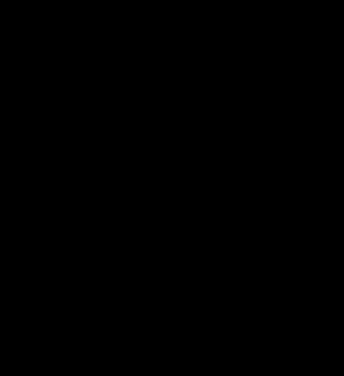
\includegraphics[width=.42\linewidth]{assets/asset-312-01.jpg}
\end{center}
\begin{choices}
  \item $3$
  \item $4$
  \item $6$
  \item $8$
\end{choices}
\begin{solution}
\textbf{答案：}C

\textbf{分析：}画出两函数在 $[0,2\pi]$ 上的图象，根据图象即可求解.

\textbf{详解：}因为函数 $y=\sin x$ 的最小正周期为 $T=2\pi$，函数 $y=2\sin\left(3x-\dfrac{\pi}{6}\right)$ 的最小正周期为 $T=\dfrac{2\pi}{3}$，所以在 $x\in[0,2\pi]$ 上函数 $y=2\sin\left(3x-\dfrac{\pi}{6}\right)$ 有三个周期的图象，在坐标系中结合五点法画出两函数图象，如图所示：由图可知，两函数图象有 6 个交点.
\end{solution}
\end{question}

\begin{question}[points=13]
\textbf{来源：}2024 年 新高考I卷，第 15 题\quad \textbf{专题：}三角形、三角函数\par
记 $\triangle ABC$ 内角 $A,B,C$ 的对边分别为 $a,b,c$，已知 $\sin C=\sqrt{2}\cos B$，$a^2+b^2-c^2=\sqrt{2}ab$.

(1) 求 $B$；

(2) 若 $\triangle ABC$ 的面积为 $3+\sqrt{3}$，求 $c$.
\begin{solution}
\textbf{答案：}(1) $B=\dfrac{\pi}{3}$ (2) $c=2\sqrt{2}$

\textbf{分析：}(1) 由余弦定理、平方关系依次求出 $\cos C,\sin C$，最后结合已知 $\sin C=\sqrt{2}\cos B$ 得 $\cos B$ 的值即可；(2) 首先求出 $A,B,C$，然后由正弦定理可将 $a,b$ 均用含有 $c$ 的式子表示，结合三角形面积公式即可列方程求解.

\textbf{详解：}(1) 由余弦定理有 $a^2+b^2-c^2=2ab\cos C$，对比已知 $a^2+b^2-c^2=\sqrt{2}ab$，可得 $\cos C=\dfrac{\sqrt{2}}{2}$，因为 $C\in(0,\pi)$，所以 $\sin C>0$，从而 $\sin C=\sqrt{1-\cos^2 C}=\dfrac{\sqrt{2}}{2}$，又因为 $\sin C=\sqrt{2}\cos B$，即 $\cos B=\dfrac{1}{2}$，注意到 $B\in(0,\pi)$，所以 $B=\dfrac{\pi}{3}$.
(2) 由(1)可得 $B=\dfrac{\pi}{3}$，$\cos C=\dfrac{\sqrt{2}}{2}$，$C\in(0,\pi)$，从而 $C=\dfrac{\pi}{4}$，$A=\pi-\dfrac{\pi}{3}-\dfrac{\pi}{4}=\dfrac{5\pi}{12}$，而 $\sin A=\sin\dfrac{5\pi}{12}=\sin\left(\dfrac{\pi}{4}+\dfrac{\pi}{6}\right)=\dfrac{\sqrt{2}}{2}\times\dfrac{\sqrt{3}}{2}+\dfrac{\sqrt{2}}{2}\times\dfrac{1}{2}=\dfrac{\sqrt{6}+\sqrt{2}}{4}$，由正弦定理有 $\dfrac{a}{\sin A}=\dfrac{b}{\sin B}=\dfrac{c}{\sin C}$，从而 $a=\dfrac{\sin A}{\sin C}\cdot c=\dfrac{\sqrt{6}+\sqrt{2}}{4}\cdot\sqrt{2}c=\dfrac{\sqrt{3}+1}{2}c$，$b=\dfrac{\sin B}{\sin C}\cdot c=\dfrac{\frac{\sqrt{3}}{2}}{\frac{\sqrt{2}}{2}}\cdot c=\dfrac{\sqrt{6}}{2}c$，由三角形面积公式可知，$\triangle ABC$ 的面积 $S=\dfrac{1}{2}ab\sin C=\dfrac{1}{2}\cdot\dfrac{\sqrt{3}+1}{2}c\cdot\dfrac{\sqrt{6}}{2}c\cdot\dfrac{\sqrt{2}}{2}=\dfrac{3+\sqrt{3}}{8}c^2$，由已知 $\triangle ABC$ 的面积为 $3+\sqrt{3}$，可得 $\dfrac{3+\sqrt{3}}{8}c^2=3+\sqrt{3}$，所以 $c=2\sqrt{2}$.
\end{solution}
\end{question}

\begin{question}[points=15]
\textbf{来源：}2024 年 新高考I卷，第 16 题\quad \textbf{专题：}三角形\par
已知 $A(0,3)$ 和 $P\left(3,\dfrac{3}{2}\right)$ 为椭圆 $C:\dfrac{x^2}{a^2}+\dfrac{y^2}{b^2}=1(a>b>0)$ 上两点.

(1) 求 $C$ 的离心率;

(2) 若过 $P$ 的直线 $l$ 交 $C$ 于另一点 $B$，且 $\triangle ABP$ 的面积为 $9$，求 $l$ 的方程.
\begin{solution}
\textbf{答案：}(1) $\dfrac{1}{2}$ (2) $3x-2y-6=0$ 或 $x-2y=0$

\textbf{分析：}(1) 代入两点得到关于 $a,b$ 的方程，解出即可；(2) 方法一：以 $AP$ 为底，求出三角形的高，即点 $B$ 到直线 $AP$ 的距离，再利用平行线距离公式得到平移后的直线方程，联立椭圆方程得到 $B$ 点坐标，则得到直线 $l$ 的方程；方法二：同法一得到点 $B$ 到直线 $AP$ 的距离，再设 $B(x_0,y_0)$，根据点到直线距离和点在椭圆上得到方程组，解出即可；法三：同法一得到点 $B$ 到直线 $AP$ 的距离，利用椭圆的参数方程即可求解；法四：首先验证直线 $AB$ 斜率不存在的情况，再设直线 $y=kx+3$，联立椭圆方程，得到点 $B$ 坐标，再利用点到直线距离公式即可；法五：首先考虑直线 $PB$ 斜率不存在的情况，再设 $PB: y-\dfrac{3}{2}=k(x-3)$，利用弦长公式和点到直线的距离公式即可得到答案；法六：设线法与法五一致，利用水平宽乘铅锤高乘 $\dfrac{1}{2}$ 表达面积即可.

\textbf{详解：}(1) 由题意得 $\begin{cases} b=3 \\ \dfrac{9}{a^2}+\dfrac{9}{4b^2}=1 \end{cases}$，解得 $b^2=9, a^2=12$，所以 $e=\sqrt{1-\dfrac{b^2}{a^2}}=\sqrt{1-\dfrac{9}{12}}=\dfrac{1}{2}$.
(2) 法一：$k_{AP}=\dfrac{\frac{3}{2}-3}{3-0}=-\dfrac{1}{2}$，则直线 $AP$ 的方程为 $y=-\dfrac{1}{2}x+3$，即 $x+2y-6=0$，$|AP|=\sqrt{(0-3)^2+\left(3-\dfrac{3}{2}\right)^2}=\dfrac{3\sqrt{5}}{2}$，由(1)知 $C:\dfrac{x^2}{12}+\dfrac{y^2}{9}=1$，设点 $B$ 到直线 $AP$ 的距离为 $d$，则 $\dfrac{1}{2}\times\dfrac{3\sqrt{5}}{2}\times d=9$，解得 $d=\dfrac{12\sqrt{5}}{5}$，则将直线 $AP$ 沿着与 $AP$ 垂直的方向平移 $\dfrac{12\sqrt{5}}{5}$ 单位即可，此时该平行线与椭圆的交点即为点 $B$，设该平行线的方程为 $x+2y+C=0$，则 $\dfrac{|C+6|}{\sqrt{5}}=\dfrac{12\sqrt{5}}{5}$，解得 $C=6$ 或 $C=-18$，当 $C=6$ 时，联立 $\begin{cases} \dfrac{x^2}{12}+\dfrac{y^2}{9}=1 \\ x+2y+6=0 \end{cases}$，解得 $\begin{cases} x=0 \\ y=-3 \end{cases}$ 或 $\begin{cases} x=-3 \\ y=-\dfrac{3}{2} \end{cases}$，即 $B(0,-3)$ 或 $B\left(-3,-\dfrac{3}{2}\right)$，当 $B(0,-3)$ 时，$k_l=\dfrac{\frac{3}{2}+3}{3-0}=\dfrac{3}{2}$，直线 $l$ 的方程为 $y=\dfrac{3}{2}x-3$，即 $3x-2y-6=0$；当 $B\left(-3,-\dfrac{3}{2}\right)$ 时，$k_l=\dfrac{\frac{3}{2}+\frac{3}{2}}{3+3}=\dfrac{1}{2}$，直线 $l$ 的方程为 $y=\dfrac{1}{2}x$，即 $x-2y=0$；当 $C=-18$ 时，联立 $\begin{cases} \dfrac{x^2}{12}+\dfrac{y^2}{9}=1 \\ x+2y-18=0 \end{cases}$ 得 $2y^2-27y+117=0$，$\Delta=27^2-4\times2\times117=-207<0$，此时直线与椭圆无交点. 综上直线 $l$ 的方程为 $3x-2y-6=0$ 或 $x-2y=0$.
\end{solution}
\end{question}

\section*{2025 年}

\begin{question}[points=5]
\textbf{来源：}2025 年 全国II卷，第 5 题\quad \textbf{专题：}三角形\par
在 $\triangle ABC$ 中，$BC=2$，$AC=1+\sqrt{3}$，$AB=\sqrt{6}$，则 $A=$（ ）
\begin{choices}
  \item $45^\circ$
  \item $60^\circ$
  \item $120^\circ$
  \item $135^\circ$
\end{choices}
\begin{solution}
\textbf{答案：}$A$

\textbf{分析：}由余弦定理 $\cos A=\frac{AB^2+AC^2-BC^2}{2AB\cdot AC}$ 直接计算求解即可.

\textbf{详解：}$\cos A=\frac{(\sqrt{6})^2+(1+\sqrt{3})^2-2^2}{2\cdot\sqrt{6}\cdot(1+\sqrt{3})}=\frac{6+1+2\sqrt{3}+3-4}{2\sqrt{6}(1+\sqrt{3})}=\frac{6+2\sqrt{3}}{2\sqrt{6}(1+\sqrt{3})}=\frac{\sqrt{2}}{2}$，又 $0^\circ<A<180^\circ$，所以 $A=45^\circ$.
\end{solution}
\end{question}

\begin{question}[points=5]
\textbf{来源：}2025 年 全国II卷，第 8 题\quad \textbf{专题：}三角函数\par
已知 $0<\alpha<\pi$，$\cos\frac{\alpha}{2}=\frac{\sqrt{5}}{5}$，则 $\sin\left(\alpha-\frac{\pi}{4}\right)=$（ ）
\begin{choices}
  \item $\frac{\sqrt{2}}{10}$
  \item $\frac{\sqrt{2}}{5}$
  \item $\frac{3\sqrt{2}}{10}$
  \item $\frac{7\sqrt{2}}{10}$
\end{choices}
\begin{solution}
\textbf{答案：}$D$

\textbf{分析：}利用二倍角余弦公式得 $\cos\alpha=-\frac{3}{5}$，则 $\sin\alpha=\frac{4}{5}$，最后再根据两角差的正弦公式即可得到答案.

\textbf{详解：}$\cos\alpha=2\cos^2\frac{\alpha}{2}-1=2\times\left(\frac{\sqrt{5}}{5}\right)^2-1=-\frac{3}{5}$，因为 $0<\alpha<\pi$，则 $\frac{\pi}{2}<\alpha<\pi$，则 $\sin\alpha=\sqrt{1-\cos^2\alpha}=\sqrt{1-\left(-\frac{3}{5}\right)^2}=\frac{4}{5}$，则 $\sin\left(\alpha-\frac{\pi}{4}\right)=\sin\alpha\cos\frac{\pi}{4}-\cos\alpha\sin\frac{\pi}{4}=\frac{4}{5}\times\frac{\sqrt{2}}{2}-\left(-\frac{3}{5}\right)\times\frac{\sqrt{2}}{2}=\frac{7\sqrt{2}}{10}$.
\end{solution}
\end{question}

\begin{question}[points=5]
\textbf{来源：}2025 年 全国II卷，第 12 题\quad \textbf{专题：}向量\par
已知平面向量 $\vec{a}=(x,1)$，$\vec{b}=(x-1,2x)$，若 $\vec{a}\perp(\vec{a}-\vec{b})$，则 $|\vec{a}|=$.
\fillin[{$\sqrt{2}$}]
\begin{solution}
\textbf{答案：}$\sqrt{2}$

\textbf{分析：}根据向量坐标化运算得 $\vec{a}-\vec{b}=(1,1-2x)$，再利用向量垂直的坐标表示得到方程，解出即可.

\textbf{详解：}$\vec{a}-\vec{b}=(1,1-2x)$，因为 $\vec{a}\perp(\vec{a}-\vec{b})$，则 $\vec{a}\cdot(\vec{a}-\vec{b})=0$，则 $x+1-2x=0$，解得 $x=1$. 则 $\vec{a}=(1,1)$，则 $|\vec{a}|=\sqrt{2}$.
\end{solution}
\end{question}

\begin{question}[points=13]
\textbf{来源：}2025 年 全国II卷，第 15 题\quad \textbf{专题：}三角函数\par
已知函数 $f(x)=\cos(2x+\varphi)$ $(0\le\varphi<\pi)$，$f(0)=\frac{1}{2}$.

（1）求 $\varphi$;

（2）设函数 $g(x)=f(x)+f\left(x-\frac{\pi}{6}\right)$，求 $g(x)$ 的值域和单调区间.
\begin{solution}
\textbf{答案：}（1）$\varphi=\frac{\pi}{3}$
（2）值域为 $[-\sqrt{3},\sqrt{3}]$；单调递减区间为 $[-\frac{\pi}{12}+k\pi,\frac{5\pi}{12}+k\pi]\ (k\in\mathbb{Z})$；单调递增区间为 $[\frac{5\pi}{12}+k\pi,\frac{11\pi}{12}+k\pi]\ (k\in\mathbb{Z})$.

\textbf{分析：}（1）直接由题意得 $\cos\varphi=\frac{1}{2},(0\le\varphi<\pi)$，结合余弦函数的单调性即可得解；（2）由三角恒等变换得 $g(x)=\sqrt{3}\cos\left(2x+\frac{\pi}{6}\right)$，由此可得值域，进一步由整体代入法可得函数的单调区间.

\textbf{详解：}（1）由题意 $f(0)=\cos\varphi=\frac{1}{2}$，且 $0\le\varphi<\pi$，所以 $\varphi=\frac{\pi}{3}$.
（2）由（1）可知 $f(x)=\cos\left(2x+\frac{\pi}{3}\right)$，所以 $g(x)=f(x)+f\left(x-\frac{\pi}{6}\right)=\cos\left(2x+\frac{\pi}{3}\right)+\cos2x=\frac{1}{2}\cos2x-\frac{\sqrt{3}}{2}\sin2x+\cos2x=\frac{3}{2}\cos2x-\frac{\sqrt{3}}{2}\sin2x=\sqrt{3}\cos\left(2x+\frac{\pi}{6}\right)$，所以函数 $g(x)$ 的值域为 $[-\sqrt{3},\sqrt{3}]$. 令 $2k\pi\le2x+\frac{\pi}{6}\le\pi+2k\pi,k\in\mathbb{Z}$，解得 $-\frac{\pi}{12}+k\pi\le x\le\frac{5\pi}{12}+k\pi,k\in\mathbb{Z}$；令 $\pi+2k\pi\le2x+\frac{\pi}{6}\le2\pi+2k\pi,k\in\mathbb{Z}$，解得 $\frac{5\pi}{12}+k\pi\le x\le\frac{11\pi}{12}+k\pi,k\in\mathbb{Z}$. 所以函数 $g(x)$ 的单调递减区间为 $[-\frac{\pi}{12}+k\pi,\frac{5\pi}{12}+k\pi]\ (k\in\mathbb{Z})$，单调递增区间为 $[\frac{5\pi}{12}+k\pi,\frac{11\pi}{12}+k\pi]\ (k\in\mathbb{Z})$.
\end{solution}
\end{question}

\begin{question}[points=15]
\textbf{来源：}2025 年 全国II卷，第 16 题\quad \textbf{专题：}三角形\par
已知椭圆 $C:\frac{x^2}{a^2}+\frac{y^2}{b^2}=1(a>b>0)$ 的离心率为 $\frac{\sqrt{2}}{2}$，长轴长为 $4$.

（1）求 $C$ 的方程；

（2）过点 $(0,-2)$ 的直线 $l$ 与 $C$ 交于 $A,B$ 两点，$O$ 为坐标原点，若 $\triangle OAB$ 的面积为 $2$，求 $|AB|$.
\begin{solution}
\textbf{答案：}（1）$\frac{x^2}{4}+\frac{y^2}{2}=1$
（2）$\sqrt{5}$

\textbf{分析：}（1）根据长轴长和离心率求出基本量后可得椭圆方程；（2）设出直线方程并联立椭圆方程后结合韦达定理用参数 $t$ 表示面积后可求 $t$ 的值，从而可求弦长.

\textbf{详解：}（1）因为长轴长为 $4$，故 $a=2$，而离心率为 $\frac{\sqrt{2}}{2}$，故 $c=\sqrt{2}$，故 $b=\sqrt{2}$，故椭圆方程为 $\frac{x^2}{4}+\frac{y^2}{2}=1$.
（2）由题设直线 $AB$ 的斜率不为 $0$，故设直线 $l:x=t(y+2)$，$A(x_1,y_1),B(x_2,y_2)$，由 $\begin{cases}x=t(y+2)\\x^2+2y^2=4\end{cases}$ 可得 $(t^2+2)y^2+4t^2y+4t^2-4=0$，故 $\Delta=16t^4-4(t^2+2)(4t^2-4)=4(8-4t^2)>0$ 即 $-\sqrt{2}<t<\sqrt{2}$，且 $y_1+y_2=-\frac{4t^2}{t^2+2}$，$y_1y_2=\frac{4t^2-4}{t^2+2}$，故 $S_{\triangle OAB}=\frac{1}{2}\times|2t|\times|y_1-y_2|=|t|\sqrt{(y_1+y_2)^2-4y_1y_2}=|t|\sqrt{\frac{16t^4}{(t^2+2)^2}-\frac{16t^2-16}{t^2+2}}=\frac{|t|\sqrt{32-16t^2}}{t^2+2}=2$，解得 $t^2=\frac{2}{3}$，即 $t=\pm\frac{\sqrt{6}}{3}$，故 $|AB|=\sqrt{1+t^2}|y_1-y_2|=\sqrt{1+\frac{2}{3}}\times\frac{\sqrt{32-16\times\frac{2}{3}}}{\frac{2}{3}+2}=\sqrt{\frac{5}{3}}\times\frac{\sqrt{\frac{64}{3}}}{\frac{8}{3}}=\frac{\sqrt{5}}{\sqrt{3}}\times\frac{8\sqrt{3}}{8}=\sqrt{5}$.
\end{solution}
\end{question}

\begin{question}[points=5]
\textbf{来源：}2025 年 全国I卷，第 4 题\quad \textbf{专题：}三角函数\par
若点 $(a,0)(a>0)$ 是函数 $y = 2\tan\left(x - \frac{\pi}{3}\right)$ 的图象的一个对称中心，则 $a$ 的最小值为（ ）
\begin{choices}
  \item $\frac{\pi}{4}$
  \item $\frac{\pi}{2}$
  \item $\frac{\pi}{3}$
  \item $\frac{4\pi}{3}$
\end{choices}
\begin{solution}
\textbf{答案：}C

\textbf{分析：}根据正切函数的对称中心的结论求解.

\textbf{详解：}根据正切函数的性质，$y = 2\tan\left(x - \frac{\pi}{3}\right)$ 的对称中心横坐标满足 $x - \frac{\pi}{3} = \frac{k\pi}{2}, k \in \mathbb{Z}$，即对称中心是 $\left(\frac{\pi}{3} + \frac{k\pi}{2}, 0\right), k \in \mathbb{Z}$，即 $a = \frac{\pi}{3} + \frac{k\pi}{2}, k \in \mathbb{Z}$，又 $a>0$，则 $k=0$ 时 $a$ 最小，最小值是 $\frac{\pi}{3}$，即 $a = \frac{\pi}{3}$. 故选：C.
\end{solution}
\end{question}

\begin{question}[points=5]
\textbf{来源：}2025 年 全国I卷，第 6 题\quad \textbf{专题：}向量\par
帆船比赛中，运动员可借助风力计测定风速的大小和方向，测出的结果在航海学中称为视风风速，视风风速对应的向量，是真风风速对应的向量与船行风速对应的向量之和，其中船行风速对应的向量与船速对应的向量大小相等，方向相反.图 1 给出了部分风力等级、名称与风速大小的对应关系.已知某帆船运动员在某时刻测得的视风风速对应的向量与船速对应的向量如图 2（风速的大小和向量的大小相同），单位（m/s），则真风为（ ）

\begin{center}
  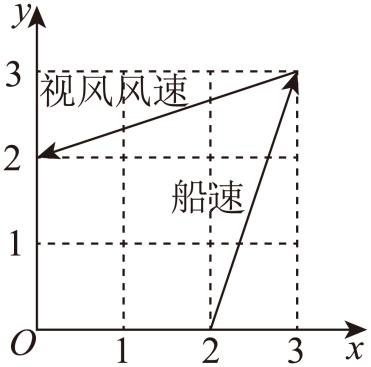
\includegraphics[width=.42\linewidth]{assets/asset-321-01.jpg}
\end{center}
\begin{choices}
  \item 轻风
  \item 微风
  \item 和风
  \item 劲风
\end{choices}
\begin{solution}
\textbf{答案：}A

\textbf{分析：}结合题目条件和图 2 写出视风风速对应的向量和船行风速对应的向量，求出真风风速对应的向量，得出真风风速的大小，即可由图 1 得出结论.

\textbf{详解：}由题意及图得，视风风速对应的向量为 $\vec{n} = (0,2) - (3,3) = (-3,-1)$，船行风速对应的向量为 $\overrightarrow{n_2} = -[(3,3)-(2,0)] = (-1,-3)$，设真风风速对应的向量为 $\overrightarrow{n_1}$，则 $\vec{n} = \overrightarrow{n_1} + \overrightarrow{n_2}$，所以 $\overrightarrow{n_1} = \vec{n} - \overrightarrow{n_2} = (-3,-1)-(-1,-3)=(-2,2)$，$|\overrightarrow{n_1}| = \sqrt{(-2)^2+2^2} = 2\sqrt{2} \approx 2.828$，所以由表得，真风风速为轻风，故选：A.
\end{solution}
\end{question}

\begin{question}[points=6]
\textbf{来源：}2025 年 全国I卷，第 11 题\quad \textbf{专题：}三角形、三角函数\par
已知 $\triangle ABC$ 的面积为 $\frac{1}{4}$，若 $\cos^2 A + \cos^2 B + 2\sin C = 2$，$\cos A \cos B \sin C = \frac{1}{4}$，则（ ）
\begin{choices}
  \item $\sin C = \sin^2 A + \sin^2 B$
  \item $AB = \sqrt{2}$
  \item $\sin A + \sin B = \frac{\sqrt{6}}{2}$
  \item $AC^2 + BC^2 = 3$
\end{choices}
\begin{solution}
\textbf{答案：}ABC

\textbf{分析：}对 $\cos^2 A + \cos^2 B + 2\sin C = 2$ 由二倍角公式先可推知 $\sin C = \sin^2 A + \sin^2 B$，然后分情况比较 $A+B$ 和 $\frac{\pi}{2}$ 的大小，结合正弦函数的单调性可推出 $C = \frac{\pi}{2}$，然后利用 $\cos A \cos B \sin C = \frac{1}{4}$ 算出 $A,B$ 取值，最后利用三角形面积求出三边长，即可判断每个选项.

\textbf{详解：}由 $\cos^2 A + \cos^2 B + 2\sin C = 2$ 得 $1-2\sin^2 A + 1-2\sin^2 B + 2\sin C = 2$，整理得 $\sin C = \sin^2 A + \sin^2 B$，A 正确；由正弦定理得 $a^2+b^2=c^2$，即 $C = \frac{\pi}{2}$，则 $\cos A \cos B = \frac{1}{4}$，又 $A+B=\frac{\pi}{2}$，所以 $\sin A \cos A = \frac{1}{4}$，即 $\sin 2A = \frac{1}{2}$，解得 $A = \frac{\pi}{12}, B = \frac{5\pi}{12}$，则 $\sin A + \sin B = \frac{\sqrt{6}-\sqrt{2}}{4} + \frac{\sqrt{6}+\sqrt{2}}{4} = \frac{\sqrt{6}}{2}$，C 正确；设 $BC = t$，则 $AC = (2+\sqrt{3})t$，$AB = (\sqrt{6}+\sqrt{2})t$，由面积公式 $\frac{1}{2} \cdot (2+\sqrt{3})t^2 = \frac{1}{4}$，解得 $t = \frac{\sqrt{3}-1}{2}$，则 $AB = (\sqrt{6}+\sqrt{2}) \cdot \frac{\sqrt{3}-1}{2} = \sqrt{2}$，B 正确；$AC^2+BC^2 = ((2+\sqrt{3})^2+1)t^2 = (8+4\sqrt{3}) \cdot \frac{(\sqrt{3}-1)^2}{4} = (8+4\sqrt{3}) \cdot \frac{4-2\sqrt{3}}{4} = (2+\sqrt{3})(4-2\sqrt{3}) = 2$，D 错误. 故选：ABC.
\end{solution}
\end{question}

\begin{question}[points=17]
\textbf{来源：}2025 年 全国I卷，第 19 题\quad \textbf{专题：}三角函数\par
设函数 $f(x) = 5\cos x - \cos 5x$.



（1）求 $f(x)$ 在 $\left[0, \frac{\pi}{4}\right]$ 的最大值；



（2）给定 $\theta \in (0,\pi)$，设 $a$ 为实数，证明：存在 $y \in [a-\theta, a+\theta]$，使得 $\cos y \le \cos \theta$；



（3）若存在 $\varphi$ 使得对任意 $x$，都有 $|5\cos x - \cos(5x+\varphi)| \le b$，求 $b$ 的最小值.
\begin{solution}
\textbf{答案：}（1）$3\sqrt{3}$；（2）证明见解析；（3）$3\sqrt{3}$

\textbf{分析：}（1）利用导数结合三角变换得导数零点，讨论导数的符号后得单调性，从而可求最大值；或者利用均值不等式可求最大值.（2）利用反证法可证三角不等式有解；（3）先考虑 $t=0,\pi$ 时 $b$ 的范围，对于 $t \in (0,\pi)$ 时，可利用（2）中的结论结合特值法求得 $b \ge 3\sqrt{3}$，从而可得 $b$ 的最小值；或者先根据函数解析特征得 $b \ge 0$，再结合特值法可得 $b \ge 3\sqrt{3}$，结合（1）的结果可得 $b$ 的最小值.

\textbf{详解：}（1）法1：$f'(x) = -5\sin x + 5\sin 5x = 10\cos 3x \sin 2x$，当 $x \in (0,\frac{\pi}{4})$ 时，$\sin 2x > 0$，$\cos 3x$ 在 $(0,\frac{\pi}{6})$ 为正，在 $(\frac{\pi}{6},\frac{\pi}{4})$ 为负，故 $f(x)$ 在 $(0,\frac{\pi}{6})$ 递增，在 $(\frac{\pi}{6},\frac{\pi}{4})$ 递减，最大值为 $f(\frac{\pi}{6}) = 5\cos\frac{\pi}{6} - \cos\frac{5\pi}{6} = 5\times\frac{\sqrt{3}}{2} - (-\frac{\sqrt{3}}{2}) = 3\sqrt{3}$. 法2：利用三角恒等变换得 $f(x)=20\cos^3 x - 16\cos^5 x$，再用均值不等式可求得最大值 $3\sqrt{3}$.
（2）法1：由余弦函数的性质得 $\cos y \le \cos\theta$ 的解为 $[2k\pi+\theta, 2k\pi+2\pi-\theta]$，$k \in \mathbb{Z}$，若每个这样的区间与 $[a-\theta, a+\theta]$ 交集为空，则 $a$ 无解，矛盾，故存在 $y \in [a-\theta, a+\theta]$ 满足条件. 法2：利用整数性质反证.
（3）记 $h(x)=5\cos x - \cos(5x+t)$，周期 $2\pi$，讨论 $t=0,\pi$ 及 $t \in (0,\pi)$ 的情形，利用（2）的结论可得 $b \ge 3\sqrt{3}$，又由（1）知 $t=0$ 时 $h(x) \le 3\sqrt{3}$，故 $b$ 的最小值为 $3\sqrt{3}$.
\end{solution}
\end{question}

\begin{question}[points=4]
\textbf{来源：}2025 年 上海卷，第 5 题\quad \textbf{专题：}三角函数\par
函数 $y = \cos x$ 在 $\left[-\frac{\pi}{2}, \frac{\pi}{4}\right]$ 上的值域为．
\fillin[{$[0,1]$}]
\begin{solution}
\textbf{答案：}$[0,1]$

\textbf{分析：}利用余弦函数的单调性可得.

\textbf{详解：}由函数 $y = \cos x$ 在 $\left[-\frac{\pi}{2}, 0\right]$ 上单调递增，在 $\left[0, \frac{\pi}{4}\right]$ 单调递减，且 $f(-\frac{\pi}{2}) = 0, f(0) = 1, f(\frac{\pi}{4}) = \frac{\sqrt{2}}{2}$，故函数 $y = \cos x$ 在 $\left[-\frac{\pi}{2}, \frac{\pi}{4}\right]$ 上的值域为 $[0,1]$ .
\end{solution}
\end{question}

\begin{question}[points=5]
\textbf{来源：}2025 年 上海卷，第 12 题\quad \textbf{专题：}向量\par
已知 $f(x) = \begin{cases} 1, & x > 0 \\ 0, & x = 0 \\ -1, & x < 0 \end{cases}$，$\vec{a}, \vec{b}, \vec{c}$ 是平面内三个不同的单位向量．若 $f(\vec{a} \cdot \vec{b}) + f(\vec{b} \cdot \vec{c}) + f(\vec{c} \cdot \vec{a}) = 0$，则 $|\vec{a} + \vec{b} + \vec{c}|$ 的取值范围是．
\fillin[{$(1, \sqrt{5})$}]
\begin{solution}
\textbf{答案：}$(1, \sqrt{5})$

\textbf{分析：}利用分段函数值分类讨论，可得 $\{f(\vec{a} \cdot \vec{b}), f(\vec{b} \cdot \vec{c}), f(\vec{c} \cdot \vec{a})\} = \{-1, 0, 1\}$，再根据数量积关系设出 $\vec{a}, \vec{b}, \vec{c}$ 坐标，利用坐标运算，结合三角恒等变换求解模的范围可得.

\textbf{详解：}若 $f(\vec{a} \cdot \vec{b}) = f(\vec{b} \cdot \vec{c}) = f(\vec{c} \cdot \vec{a}) = 0$，则 $\vec{a} \cdot \vec{b} = \vec{b} \cdot \vec{c} = \vec{c} \cdot \vec{a} = 0$，又三个向量均为平面内的单位向量，故向量 $\vec{a}, \vec{b}, \vec{c}$ 两两垂直，显然不成立；故 $\{f(\vec{a} \cdot \vec{b}), f(\vec{b} \cdot \vec{c}), f(\vec{c} \cdot \vec{a})\} = \{-1, 0, 1\}$ . 不妨设 $\begin{cases} f(\vec{a} \cdot \vec{b}) = 1 \\ f(\vec{b} \cdot \vec{c}) = 0 \\ f(\vec{c} \cdot \vec{a}) = -1 \end{cases}$，则 $\vec{a} \cdot \vec{b} > 0, \vec{b} \cdot \vec{c} = 0, \vec{c} \cdot \vec{a} < 0$，不妨设 $\vec{b} = (1,0), \vec{c} = (0,1)$，$\vec{a} = (\cos \theta, \sin \theta), \theta \in [0, 2\pi)$，则 $\begin{cases} \vec{a} \cdot \vec{b} = \cos \theta > 0 \\ \vec{c} \cdot \vec{a} = \sin \theta < 0 \end{cases}$，则 $\theta \in \left(\frac{3\pi}{2}, 2\pi\right)$，则 $|\vec{a} + \vec{b} + \vec{c}| = \sqrt{(1+\cos \theta)^2 + (1+\sin \theta)^2} = \sqrt{3 + 2\cos \theta + 2\sin \theta} = \sqrt{3 + 2\sqrt{2}\sin\left(\theta + \frac{\pi}{4}\right)}$，由 $\theta \in \left(\frac{3\pi}{2}, 2\pi\right)$，$\theta + \frac{\pi}{4} \in \left(\frac{7\pi}{4}, \frac{9\pi}{4}\right)$，则 $\sin\left(\theta + \frac{\pi}{4}\right) \in \left(-\frac{\sqrt{2}}{2}, \frac{\sqrt{2}}{2}\right)$，$2\sqrt{2}\sin\left(\theta + \frac{\pi}{4}\right) \in (-2, 2)$，故 $|\vec{a} + \vec{b} + \vec{c}| \in (1, \sqrt{5})$ .
\end{solution}
\end{question}

\begin{question}[points=5]
\textbf{来源：}2025 年 上海卷，第 15 题\quad \textbf{专题：}三角形\par
已知 $A(0,1), B(1,2)$，$C$ 在 $\Gamma: x^2 - y^2 = 1 (x \geq 1, y \geq 0)$ 上，则 $\triangle ABC$ 的面积（ ）
\begin{choices}
  \item 有最大值，但没有最小值
  \item 没有最大值，但有最小值
  \item 既有最大值，也有最小值
  \item 既没有最大值，也没有最小值
\end{choices}
\begin{solution}
\textbf{答案：}A

\textbf{分析：}设出曲线上一点为 $(a, b)$，得出 $a = \sqrt{b^2 + 1}$，将三角形的高转化成关于 $b$ 的函数，分析其单调性，从而求解.

\textbf{详解：}设曲线上一点为 $(a, b)$，则 $a^2 - b^2 = 1$，则 $a = \sqrt{b^2 + 1}$，$k_{AB} = \frac{2-1}{1-0} = 1$，$AB$ 方程为：$y-1 = x$，即 $x - y + 1 = 0$，根据点到直线的距离公式，$(a, b)$ 到 $AB$ 的距离为：$\frac{|a - b + 1|}{\sqrt{2}} = \frac{\sqrt{b^2 + 1} - b + 1}{\sqrt{2}}$，设 $f(b) = \sqrt{b^2 + 1} - b = \frac{1}{\sqrt{b^2 + 1} + b}$，由于 $b \geq 0$，显然 $f(b)$ 关于 $b$ 单调递减，$f(b)_{\max} = f(0)$，无最小值，即 $\triangle ABC$ 中，$AB$ 边上的高有最大值，无最小值，又 $AB$ 一定，故面积有最大值，无最小值. 故选：A.
\end{solution}
\end{question}

\begin{question}[points=5]
\textbf{来源：}2025 年 上海卷，第 16 题\quad \textbf{专题：}三角形\par
已知数列 $\{a_n\}$、$\{b_n\}$、$\{c_n\}$ 的通项公式分别为 $a_n = 10n - 9$，$b_n = 2^n$，$c_n = \lambda a_n + (1-\lambda)b_n$．若对任意的 $\lambda \in [0,1]$，$a_n$、$b_n$、$c_n$ 的值均能构成三角形，则满足条件的正整数 $n$ 有（ ）
\begin{choices}
  \item $4$ 个
  \item $3$ 个
  \item $1$ 个
  \item 无数个
\end{choices}
\begin{solution}
\textbf{答案：}B

\textbf{分析：}由 $c_n = \lambda a_n + (1-\lambda)b_n$ 可知 $c_n$ 范围，再由三角形三边关系可得 $a_n, b_n, c_n$ 的不等关系，结合函数零点解不等式可得.

\textbf{详解：}由题意 $a_n, b_n, c_n > 0$，不妨设 $A(n, a_n), B(n, b_n), C(n, c_n)$，三点均在第一象限内，由 $c_n = \lambda a_n + (1-\lambda)b_n$ 可知，$\overrightarrow{BC} = \lambda \overrightarrow{BA}, \lambda \in [0,1]$，故点 $C$ 恒在线段 $AB$ 上，则有 $\min\{a_n, b_n\} \leq c_n \leq \max\{a_n, b_n\} < a_n + b_n$．即对任意的 $\lambda \in [0,1]$，$c_n < a_n + b_n$ 恒成立，令 $10x - 9 = 2^x$，构造函数 $f(x) = 2^x - 10x + 9, x > 0$，则 $f'(x) = 2^x \ln 2 - 10$，由 $f'(x)$ 单调递增，又 $f'(3) < 0, f'(4) > 0$，存在 $x_0 \in (3,4)$，使 $f'(x_0) = 0$，即当 $0 < x < x_0$ 时，$f'(x) < 0$，$f(x)$ 单调递减；当 $x > x_0$ 时，$f'(x) > 0$，$f(x)$ 单调递增；故 $f(x)$ 至多 $2$ 个零点，又由 $f(1) > 0, f(2) < 0, f(5) < 0, f(6) > 0$，可知 $f(x)$ 存在 $2$ 个零点，不妨设 $x_1, x_2 (x_1 < x_2)$，且 $x_1 \in (1,2), x_2 \in (5,6)$．①若 $a_n \leq b_n$，即 $10n - 9 \leq 2^n$ 时，此时 $n = 1$ 或 $n \geq 6$．则 $a_n \leq c_n \leq b_n$，可知 $b_n + c_n > a_n$ 成立，要使 $a_n$、$b_n$、$c_n$ 的值均能构成三角形，所以 $a_n + c_n > b_n$ 恒成立，故 $b_n < 2a_n$，所以有 $\begin{cases} 10n - 9 \leq 2^n \\ 2^n < 2(10n - 9) \end{cases}$，解得 $n = 6$；②若 $a_n \geq b_n$，即 $10n - 9 \geq 2^n$ 时，此时 $n = 2,3,4,5$．则 $a_n \geq c_n \geq b_n$，可知 $a_n + c_n > b_n$ 成立，要使 $a_n$、$b_n$、$c_n$ 的值均能构成三角形，所以 $b_n + c_n > a_n$ 恒成立，故 $a_n < 2b_n$，所以有 $\begin{cases} 10n - 9 \geq 2^n \\ 10n - 9 < 2^{n+1} \end{cases}$，解得 $n = 4$ 或 $5$；综上可知，正整数 $n$ 的个数有 $3$ 个. 故选：B.
\end{solution}
\end{question}

\begin{question}[points=18]
\textbf{来源：}2025 年 上海卷，第 20 题\quad \textbf{专题：}向量\par
已知椭圆 $\Gamma: \frac{x^2}{a^2} + \frac{y^2}{5} = 1 (a > \sqrt{5})$，$M(0, m) (m > 0)$，$A$ 是 $\Gamma$ 的右顶点．

(1) 若 $\Gamma$ 的焦点 $(2,0)$，求离心率 $e$；

(2) 若 $a = 4$，且 $\Gamma$ 上存在一点 $P$，满足 $\overrightarrow{PA} = 2\overrightarrow{MP}$，求 $m$；

(3) 已知 $AM$ 的中垂线 $l$ 的斜率为 $2$，$l$ 与 $\Gamma$ 交于 $C$、$D$ 两点，$\angle CMD$ 为钝角，求 $a$ 的取值范围．
\begin{solution}
\textbf{答案：}(1) $\frac{2}{3}$； (2) $\sqrt{10}$； (3) $(\sqrt{5}, \sqrt{11})$

\textbf{分析：}(1) 由方程可得 $b^2 = 5$，再由焦点坐标得 $c$，从而求出 $a$ 得离心率； (2) 设点 $P$ 坐标，由向量关系 $\overrightarrow{PA} = 2\overrightarrow{MP}$ 坐标化可解得 $P$ 坐标，代入椭圆方程可得 $m$； (3) 根据中垂线性质，由斜率与中点坐标得直线 $l$ 方程，联立直线与椭圆方程，将钝角条件转化为向量不等式 $\overrightarrow{MC} \cdot \overrightarrow{MD} < 0$，再坐标化利用韦达定理代入化简不等式求解可得 $a$ 范围.

\textbf{详解：}(1) 由题意知，$\Gamma: \frac{x^2}{a^2} + \frac{y^2}{5} = 1 (a > \sqrt{5})$，则 $b^2 = 5$，由右焦点 $(2,0)$，可知 $c = 2$，则 $a = \sqrt{5 + c^2} = 3$，故离心率 $e = \frac{c}{a} = \frac{2}{3}$．
(2) 由题意 $A(4,0), M(0, m) (m > 0)$，$P(x_P, y_P)$，由 $\overrightarrow{PA} = 2\overrightarrow{MP}$ 得，$\begin{cases} 4 - x_P = 2x_P \\ -y_P = 2y_P - 2m \end{cases}$，解得 $P\left(\frac{4}{3}, \frac{2m}{3}\right)$，代入 $\frac{x^2}{16} + \frac{y^2}{5} = 1$，得 $\frac{1}{9} + \frac{4m^2}{45} = 1$，又 $m > 0$，解得 $m = \sqrt{10}$．
(3) 由线段 $AM$ 的中垂线 $l$ 的斜率为 $2$，所以直线 $AM$ 的斜率为 $-\frac{1}{2}$，则 $\frac{m-0}{0-a} = -\frac{1}{2}$，解得 $m = \frac{a}{2}$，由 $A(a,0), M(0, \frac{a}{2})$ 得 $AM$ 中点坐标为 $(\frac{a}{2}, \frac{a}{4})$，故直线 $l: y = 2x - \frac{3}{4}a$，显然直线 $l$ 过椭圆内点 $(\frac{3}{8}a, 0)$，故直线与椭圆恒有两不同交点，设 $C(x_1, y_1), D(x_2, y_2)$，由 $\begin{cases} y = 2x - \frac{3}{4}a \\ 5x^2 + a^2 y^2 = 5a^2 \end{cases}$ 消 $y$ 得 $(4a^2 + 5)x^2 - 3a^3 x + \frac{9}{16}a^4 - 5a^2 = 0$，由韦达定理得 $x_1 + x_2 = \frac{3a^3}{4a^2 + 5}$，$x_1 x_2 = \frac{\frac{9}{16}a^4 - 5a^2}{4a^2 + 5}$．因为 $\angle CMD$ 为钝角，则 $\overrightarrow{MC} \cdot \overrightarrow{MD} < 0$，且 $M(0, \frac{a}{2})$，则有 $x_1 x_2 + (y_1 - \frac{a}{2})(y_2 - \frac{a}{2}) < 0$，所以 $x_1 x_2 + \left(2x_1 - \frac{5a}{4}\right)\left(2x_2 - \frac{5a}{4}\right) = 5x_1 x_2 - \frac{5a}{2}(x_1 + x_2) + \frac{25}{16}a^2 < 0$，即 $5\left(\frac{\frac{9}{16}a^4 - 5a^2}{4a^2 + 5}\right) - \frac{5a}{2} \cdot \frac{3a^3}{4a^2 + 5} + \frac{25}{16}a^2 < 0$，解得 $a^2 < 11$，又 $a > \sqrt{5}$，故 $\sqrt{5} < a < \sqrt{11}$，即 $a$ 的取值范围是 $(\sqrt{5}, \sqrt{11})$．
\end{solution}
\end{question}

\begin{question}[points=18]
\textbf{来源：}2025 年 上海卷，第 21 题\quad \textbf{专题：}三角函数\par
已知函数 $y = f(x)$ 的定义域为 $\mathbf{R}$．对于正实数 $a$，定义集合 $M_a = \{x \mid f(x+a) = f(x)\}$．

(1) 若 $f(x) = \sin x$，判断 $\frac{\pi}{3}$ 是否是 $M_\pi$ 中的元素，请说明理由；

(2) 若 $f(x) = \begin{cases} x+2, & x < 0 \\ x, & x \geq 0 \end{cases}$，$M_a \neq \varnothing$，求 $a$ 的取值范围；

(3) 若 $y = f(x)$ 是偶函数，当 $x \in (0,1]$ 时，$f(x) = 1 - x$，且对任意 $a \in (0,2)$，均有 $M_a \subseteq M_2$．写出 $y = f(x)$，$x \in (1,2)$ 解析式，并证明：对任意实数 $c$，函数 $y = f(x) - c$ 在 $[-3,3]$ 上至多有 $9$ 个零点．
\begin{solution}
\textbf{答案：}(1) 不是； (2) $\left[\frac{7}{4}, 4\right)$； (3) 解析式 $f(x) = x - 1, x \in (1,2)$；证明见解析

\textbf{分析：}(1) 直接代入计算 $f\left(\frac{\pi}{3}\right)$ 和 $f\left(\frac{\pi}{3} + \pi\right)$ 即可； (2) 法一：转化为存在实数 $x_0$ 使得 $f(x_0 + a) = f(x_0)$，分析得 $x_0 + 2 = \sqrt{x_0 + a}$，再计算得 $a = (x_0 + 2)^2 - x_0 = \left(x_0 + \frac{3}{2}\right)^2 + \frac{7}{4}$，最后根据 $x_0$ 的范围即可得到答案；法二：画出函数图象，转化为直线 $y = t$ 与该函数有两个交点，将 $a$ 用 $t$ 表示，最后利用二次函数性质即可得到答案； (3) 利用函数奇偶性和集合新定义即可求出 $x \in (1,2)$ 时解析式，再分析出 $f(-3) \notin (0,1)$，最后对 $c$ 的范围进行分类讨论即可.

\textbf{详解：}(1) $f\left(\frac{\pi}{3}\right) = \sin\frac{\pi}{3} = \frac{\sqrt{3}}{2}$，$f\left(\frac{\pi}{3} + \pi\right) = -\sin\frac{\pi}{3} = -\frac{\sqrt{3}}{2}$，两者不相等，故 $\frac{\pi}{3}$ 不是 $M_\pi$ 中的元素．
(2) 法一：因为 $M_a \neq \varnothing$，则存在实数 $x_0$ 使得 $f(x_0 + a) = f(x_0)$，且 $a > 0$，当 $x < 0$ 时，$f(x) = x+2$，其在 $(-\infty, 0)$ 上严格单调递增，当 $x \geq 0$ 时，$f(x) = \sqrt{x}$，其在 $[0, +\infty)$ 上也严格单调递增，则 $x_0 < 0 \leq x_0 + a$，则 $x_0 + 2 = \sqrt{x_0 + a}$，令 $x+2 = 0$，解得 $x = -2$，则 $-2 \leq x_0 < 0$，则 $a = (x_0 + 2)^2 - x_0 = \left(x_0 + \frac{3}{2}\right)^2 + \frac{7}{4} \in \left[\frac{7}{4}, 4\right)$．法二：作出该函数图象，则由题意知直线 $y = t$ 与该函数有两个交点，由图知 $0 \leq t < 2$，假设交点分别为 $A(m, t)$，$B(n, t)$，联立方程组 $\begin{cases} m = t^2 \\ n+2 = t \end{cases}$ 得 $a = |AB| = m - n = t^2 - (t-2) = \left(t - \frac{1}{2}\right)^2 + \frac{7}{4} \in \left[\frac{7}{4}, 4\right)$．
(3) 对任意 $x_0 \in (1,2)$，$x_0 - 2 \in (-1,0)$，因为其是偶函数，则 $f(x_0 - 2) = f(2 - x_0)$，而 $4 - 2x_0 \in (0,2)$，所以 $x_0 - 2 \in M_{4-2x_0} \subseteq M_2$，所以 $f(x_0) = f(x_0 - 2) = f(2 - x_0)$，因为 $x_0 \in (1,2)$，则 $2 - x_0 \in (0,1)$，所以 $f(x_0) = f(2 - x_0) = 1 - (2 - x_0) = x_0 - 1$，所以 $f(x) = x - 1, x \in (1,2)$．所以当 $s \in (0,1)$ 时，$1-s \in (0,1)$，$1+s \in (1,2)$，则 $f(1-s) = 1 - (1-s) = s$，$f(1+s) = (1+s) - 1 = s$，则 $f(1-s) = f(1+s)$，而 $1+s - (1-s) = 2s$，$(3-s) - (1-s) = 2$，则 $1-s \in M_{2s} \subseteq M_2$，则 $f(1-s) = f(3-s)$，所以当 $x \in (2,3)$ 时，$f(x) = f(x-2) = 1 - (x-2) = 3 - x$，而 $f(x)$ 为偶函数，画出函数图象如下：其中 $f(-3) = f(3)$，$f(-2) = f(2)$，$f(0)$，但其对应的 $y$ 值均未知．首先说明 $f(-3) = n \notin (0,1)$，若 $f(-3) = n \in (0,1)$，则 $-3+n \in (-3,-2)$，易知此时 $f(x) = x+3, x \in (-3,-2)$，则 $f(-3+n) = n$，所以 $f(-3) \in M_n \subseteq M_2$，而 $x \in [-1,0)$ 时，$f(x) = x+1$，所以 $f(-3) = f(-1) = 0$，与 $f(-3) = n$ 矛盾，所以 $f(-3) \notin (0,1)$，即 $f(-3) = f(3) \notin (0,1)$．令 $y = f(x) - c = 0$，则 $y = f(x) = c$，当 $c = 0$ 时，即使让 $f(-3) = f(3) = f(-2) = f(2) = f(0) = 0$，此时最多 $7$ 个零点；当 $c \geq 1$ 时，若 $f(-2) = f(2) = f(0) = f(-3) = f(3) = c$，此时有 $5$ 个零点，故此时最多 $5$ 个零点；当 $c < 0$ 时，若 $f(-2) = f(2) = f(0) = f(-3) = f(3) = c$，此时有 $5$ 个零点，故此时最多 $5$ 个零点；当 $0 < c < 1$ 时，若 $f(-2) = f(2) = f(0) = c$，此时有 $3$ 个零点，若 $f(-3) = c \in (0,1)$，则 $-3+c \in (-3,-2)$，易知此时 $f(x) = x+3$，则 $f(-3+c) = c$，所以 $f(-3) \in M_c \subseteq M_2$，而 $x \in [-1,0)$ 时，$f(x) = x+1$，所以 $f(-3) = f(-1) = 0$，与 $f(-3) = c$ 矛盾，所以 $f(-3) \notin (0,1)$，则最多在 $(-3,-2), (-2,-1), (-1,0), (0,1), (1,2), (2,3)$ 之间取得 $6$ 个零点，以及在 $x = -2, 0, 2$ 处成为零点，故不超过 $9$ 个零点．综上，零点不超过 $9$ 个.
\end{solution}
\end{question}

\begin{question}[points=5]
\textbf{来源：}2025 年 天津卷，第 2 题\quad \textbf{专题：}三角函数\par
设$x \in \mathbb{R}$, 则“$x = 0$”是“$\sin 2x = 0$”的（   ）
\begin{choices}
  \item 充分不必要条件
  \item 必要不充分条件
  \item 充要条件
  \item 既不充分也不必要条件
\end{choices}
\begin{solution}
\textbf{答案：}A

\textbf{分析：}通过判断是否能相互推出，由充分条件与必要条件的定义可得.

\textbf{详解：}由$x = 0 \Rightarrow \sin 2x = \sin 0 = 0$, 则“$x = 0$”是“$\sin 2x = 0$”的充分条件；又当$x = \pi$时, $\sin 2x = \sin 2\pi = 0$, 可知$\sin 2x = 0 \not\Rightarrow x = 0$, 故“$x = 0$”不是“$\sin 2x = 0$”的必要条件. 综上可知, “$x = 0$”是“$\sin 2x = 0$”的充分不必要条件. 故选A.
\end{solution}
\end{question}

\begin{question}[points=5]
\textbf{来源：}2025 年 天津卷，第 8 题\quad \textbf{专题：}三角函数\par
$f(x) = \sin(\omega x + \varphi)$ ($\omega > 0$, $-\pi < \varphi < \pi$), 在$\left[-\dfrac{5\pi}{12}, \dfrac{\pi}{12}\right]$上单调递增, 且$x = \dfrac{\pi}{12}$为它的一条对称轴, $\left(\dfrac{\pi}{3}, 0\right)$是它的一个对称中心, 当$x \in \left[0, \dfrac{\pi}{2}\right]$时, $f(x)$的最小值为（   ）
\begin{choices}
  \item $-\dfrac{\sqrt{3}}{2}$
  \item $-\dfrac{1}{2}$
  \item 1
  \item 0
\end{choices}
\begin{solution}
\textbf{答案：}A

\textbf{分析：}利用正弦函数的对称性得出$\omega = 4n + 2$, 根据单调性得出$0 < \omega \le 2$, 从而确定$\omega$, 结合对称轴与对称中心再求出$\varphi$, 得出函数解析式, 利用整体思想及正弦函数的性质即可得解.

\textbf{详解：}设$f(x)$的最小正周期为$T$, 根据题意有$\begin{cases} \dfrac{\pi}{12}\omega + \varphi = \dfrac{\pi}{2} + 2k\pi \\ \dfrac{\pi}{3}\omega + \varphi = m\pi \end{cases}$, $(m, k \in \mathbb{Z})$. 由正弦函数的对称性可知$\dfrac{\pi}{3} - \dfrac{\pi}{12} = \dfrac{(2n+1)T}{4}$ ($n \in \mathbb{Z}$), 即$\dfrac{\pi}{4} = \dfrac{2n\pi + \pi}{2\omega}$, $\therefore \omega = 4n + 2$. 又$f(x)$在$\left[-\dfrac{5\pi}{12}, \dfrac{\pi}{12}\right]$上单调递增, 则$\dfrac{T}{2} \ge \dfrac{\pi}{12} - \left(-\dfrac{5\pi}{12}\right)$, $\therefore \dfrac{\pi}{\omega} \ge \dfrac{\pi}{2} \Rightarrow 0 < \omega \le 2$. $\therefore \omega = 2$, 则$\begin{cases} \varphi = \dfrac{\pi}{3} + 2k\pi \\ \varphi = m\pi - \dfrac{2\pi}{3} \end{cases}$. $\because \varphi \in (-\pi, \pi)$, $\therefore k=0$, $m=1$时, $\varphi = \dfrac{\pi}{3}$, $\therefore f(x) = \sin\left(2x + \dfrac{\pi}{3}\right)$. 当$x \in \left[0, \dfrac{\pi}{2}\right]$时, $2x + \dfrac{\pi}{3} \in \left[\dfrac{\pi}{3}, \dfrac{4\pi}{3}\right]$, 由正弦函数的单调性可知$f(x)_{\min} = \sin\dfrac{4\pi}{3} = -\dfrac{\sqrt{3}}{2}$. 故选A.
\end{solution}
\end{question}

\begin{question}[points=5]
\textbf{来源：}2025 年 天津卷，第 14 题\quad \textbf{专题：}向量\par
$\triangle ABC$中, $D$为$AB$边中点, $\overrightarrow{CE} = \dfrac{1}{3}\overrightarrow{CD}$, $\overrightarrow{AB} = \vec{a}$, $\overrightarrow{AC} = \vec{b}$, 则$\overrightarrow{AE} = $（用$\vec{a}$, $\vec{b}$表示）, 若$|\overrightarrow{AE}| = 5$, $\overrightarrow{AE} \perp \overrightarrow{CB}$, 则$\overrightarrow{AE} \cdot \overrightarrow{CD} = $.
\fillin[{$\dfrac{1}{6}\vec{a} + \dfrac{2}{3}\vec{b}$；$-15$}]
\begin{solution}
\textbf{答案：}$\dfrac{1}{6}\vec{a} + \dfrac{2}{3}\vec{b}$；$-15$

\textbf{分析：}根据向量的线性运算求解即可空一，应用数量积运算律计算求解空二.

\textbf{详解：}如图，因为$\overrightarrow{CE} = \dfrac{1}{3}\overrightarrow{CD}$, 所以$\overrightarrow{AE} - \overrightarrow{AC} = \dfrac{1}{3}(\overrightarrow{AD} - \overrightarrow{AC})$, 所以$\overrightarrow{AE} = \dfrac{1}{3}\overrightarrow{AD} + \dfrac{2}{3}\overrightarrow{AC}$. 因为$D$为线段$AB$的中点, 所以$\overrightarrow{AE} = \dfrac{1}{6}\overrightarrow{AB} + \dfrac{2}{3}\overrightarrow{AC} = \dfrac{1}{6}\vec{a} + \dfrac{2}{3}\vec{b}$. 又因为$|\overrightarrow{AE}| = 5$, $\overrightarrow{AE} \perp \overrightarrow{CB}$, 所以$|\overrightarrow{AE}|^2 = \left(\dfrac{1}{6}\vec{a} + \dfrac{2}{3}\vec{b}\right)^2 = \dfrac{1}{36}|\vec{a}|^2 + \dfrac{2}{9}\vec{a}\cdot\vec{b} + \dfrac{4}{9}|\vec{b}|^2 = 25$, $\overrightarrow{AE} \cdot \overrightarrow{CB} = \left(\dfrac{1}{6}\vec{a} + \dfrac{2}{3}\vec{b}\right)\cdot(\vec{a} - \vec{b}) = \dfrac{1}{6}|\vec{a}|^2 + \dfrac{1}{2}\vec{a}\cdot\vec{b} - \dfrac{2}{3}|\vec{b}|^2 = 0$, 所以$|\vec{a}|^2 + 3\vec{a}\cdot\vec{b} = 4|\vec{b}|^2$. 所以$|\vec{a}|^2 + 4\vec{a}\cdot\vec{b} = 180$, 所以$\overrightarrow{AE} \cdot \overrightarrow{CD} = \left(\dfrac{1}{6}\vec{a} + \dfrac{2}{3}\vec{b}\right)\cdot\left(-\vec{b} + \dfrac{1}{2}\vec{a}\right) = \dfrac{1}{12}|\vec{a}|^2 + \dfrac{1}{6}\vec{a}\cdot\vec{b} - \dfrac{2}{3}|\vec{b}|^2 = \dfrac{1}{12}(|\vec{a}|^2 + 2\vec{a}\cdot\vec{b} - 8|\vec{b}|^2) = \dfrac{1}{12}(|\vec{a}|^2 + 2\vec{a}\cdot\vec{b} - 2(|\vec{a}|^2 + 3\vec{a}\cdot\vec{b})) = \dfrac{1}{12}(-|\vec{a}|^2 - 4\vec{a}\cdot\vec{b}) = -\dfrac{1}{12}(|\vec{a}|^2 + 4\vec{a}\cdot\vec{b}) = -\dfrac{180}{12} = -15$. 故答案为$\dfrac{1}{6}\vec{a} + \dfrac{2}{3}\vec{b}$；$-15$.
\end{solution}
\end{question}

\begin{question}[points=15]
\textbf{来源：}2025 年 天津卷，第 16 题\quad \textbf{专题：}三角形、三角函数\par
在$\triangle ABC$中, 角$A, B, C$的对边分别为$a, b, c$. 已知$a\sin B = \sqrt{3}b\cos A$, $c - 2b = 1$, $a = \sqrt{7}$.

(1) 求$A$的值;

(2) 求$c$的值;

(3) 求$\sin(A + 2B)$的值.
\begin{solution}

\textbf{分析：}(1)由正弦定理化边为角再化简可求；(2)由余弦定理，结合(1)结论与已知代入可得关于$b$的方程，求解可得$b$，进而求得$c$；(3)利用正弦定理先求$B$，再由二倍角公式分别求$\sin 2B$, $\cos 2B$，由两角和的正弦可得.

\textbf{详解：}（1）已知$a\sin B = \sqrt{3}b\cos A$, 由正弦定理$\dfrac{a}{\sin A} = \dfrac{b}{\sin B}$, 得$a\sin B = b\sin A = \sqrt{3}b\cos A$, 显然$\cos A \neq 0$, 得$\tan A = \sqrt{3}$, 由$0 < A < \pi$, 故$A = \dfrac{\pi}{3}$.
（2）由（1）知$\cos A = \dfrac{1}{2}$, 且$c = 2b + 1$, $a = \sqrt{7}$, 由余弦定理$a^2 = b^2 + c^2 - 2bc\cos A$, 则$7 = b^2 + (2b+1)^2 - 2 \times \dfrac{1}{2} b(2b+1) = 3b^2 + 3b + 1$, 解得$b = 1$（$b = -2$舍去）, 故$c = 3$.
（3）由正弦定理$\dfrac{a}{\sin A} = \dfrac{b}{\sin B}$, 且$b = 1$, $a = \sqrt{7}$, $\sin A = \dfrac{\sqrt{3}}{2}$, 得$\sin B = \dfrac{b\sin A}{a} = \dfrac{\sqrt{21}}{14}$, 且$a > b$, 则$B$为锐角, 故$\cos B = \dfrac{5\sqrt{7}}{14}$, 故$\sin 2B = 2\sin B\cos B = \dfrac{5\sqrt{3}}{14}$, 且$\cos 2B = 1 - 2\sin^2 B = 1 - 2 \times \left(\dfrac{\sqrt{21}}{14}\right)^2 = \dfrac{11}{14}$; 故$\sin(A + 2B) = \sin A \cos 2B + \cos A \sin 2B = \dfrac{\sqrt{3}}{2} \times \dfrac{11}{14} + \dfrac{1}{2} \times \dfrac{5\sqrt{3}}{14} = \dfrac{4\sqrt{3}}{7}$.
\end{solution}
\end{question}

\begin{question}[points=15]
\textbf{来源：}2025 年 天津卷，第 18 题\quad \textbf{专题：}三角形\par
已知椭圆$\dfrac{x^2}{a^2} + \dfrac{y^2}{b^2} = 1$ ($a > b > 0$)的左焦点为$F$, 右顶点为$A$, $P$为$x = a$上一点, 且直线$PF$的斜率为$\dfrac{1}{3}$, $\triangle PFA$的面积为$\dfrac{3}{2}$, 离心率为$\dfrac{1}{2}$.

(1) 求椭圆的方程;

(2) 过点$P$的直线与椭圆有唯一交点$B$（异于点$A$）, 求证: $PF$平分$\angle AFB$.
\begin{solution}

\textbf{分析：}(1)根据题意，利用椭圆的离心率得到$a=2c$，再由直线$PF$的斜率得到$m=c$，从而利用三角形的面积公式得到关于$c$的方程，解之即可得解；(2)联立直线与椭圆方程，利用其位置关系求得$k$，进而得到直线$PB$的方程与点$B$的坐标，法一：利用向量的夹角公式即可得证；法二：利用两直线的夹角公式即可得证；法三利用正切的倍角公式即可得证；法四：利用角平分线的性质与点线距离公式即可得证.

\textbf{详解：}（1）依题意，设椭圆$\dfrac{x^2}{a^2} + \dfrac{y^2}{b^2} = 1$ ($a > b > 0$)的半焦距为$c$, 则左焦点$F(-c,0)$, 右顶点$A(a,0)$, 离心率$e = \dfrac{c}{a} = \dfrac{1}{2}$, 即$a = 2c$. 因为$P$为$x = a$上一点, 设$P(a,m)$, 又直线$PF$的斜率为$\dfrac{1}{3}$, 则$\dfrac{m - 0}{a - (-c)} = \dfrac{1}{3}$, 即$\dfrac{m}{2c + c} = \dfrac{1}{3}$, 解得$m = c$, 则$P(a,c)$, 即$P(2c,c)$. 因为$\triangle PFA$的面积为$\dfrac{3}{2}$, $|AF| = a - (-c) = a + c = 3c$, 高为$|m| = c$, 所以$S_{\triangle PFA} = \dfrac{1}{2} |AF| |m| = \dfrac{1}{2} \times 3c \times c = \dfrac{3}{2}$, 解得$c = 1$, 则$a = 2c = 2$, $b^2 = a^2 - c^2 = 3$, 所以椭圆的方程为$\dfrac{x^2}{4} + \dfrac{y^2}{3} = 1$.
（2）由(1)可知$P(2,1)$, $F(-1,0)$, $A(2,0)$. 易知直线$PB$的斜率存在, 设其方程为$y = kx + m$, 则$1 = 2k + m$, 即$m = 1 - 2k$. 联立$\begin{cases} y = kx + m \\ \dfrac{x^2}{4} + \dfrac{y^2}{3} = 1 \end{cases}$, 消去$y$得, $(3 + 4k^2)x^2 + 8kmx + 4m^2 - 12 = 0$. 因为直线与椭圆有唯一交点, 所以$\Delta = (8km)^2 - 4(3+4k^2)(4m^2 - 12) = 0$, 即$4k^2 - m^2 + 3 = 0$, 则$4k^2 - (1 - 2k)^2 + 3 = 0$, 解得$k = -\dfrac{1}{2}$, 则$m = 2$, 所以直线$PB$的方程为$y = -\dfrac{1}{2}x + 2$. 联立$\begin{cases} y = -\dfrac{1}{2}x + 2 \\ \dfrac{x^2}{4} + \dfrac{y^2}{3} = 1 \end{cases}$, 解得$\begin{cases} x = 1 \\ y = \dfrac{3}{2} \end{cases}$, 则$B(1, \dfrac{3}{2})$. 以下分别用四种方法证明结论：
法一：则$\overrightarrow{FB} = \left(2, \dfrac{3}{2}\right)$, $\overrightarrow{FP} = (3,1)$, $\overrightarrow{FA} = (3,0)$. 所以$\cos\angle BFP = \dfrac{\overrightarrow{FB} \cdot \overrightarrow{FP}}{|\overrightarrow{FB}||\overrightarrow{FP}|} = \dfrac{2 \times 3 + \dfrac{3}{2} \times 1}{\sqrt{2^2 + \left(\dfrac{3}{2}\right)^2} \times \sqrt{3^2 + 1^2}} = \dfrac{3\sqrt{10}}{10}$, $\cos\angle PFA = \dfrac{\overrightarrow{FA} \cdot \overrightarrow{FP}}{|\overrightarrow{FA}||\overrightarrow{FP}|} = \dfrac{3 \times 3 + 1 \times 0}{3 \times \sqrt{3^2 + 1^2}} = \dfrac{3\sqrt{10}}{10}$, 则$\cos\angle BFP = \cos\angle PFA$, 又$\angle BFP, \angle PFA \in (0, \dfrac{\pi}{2})$, 所以$\angle BFP = \angle PFA$, 即$PF$平分$\angle AFB$.
法二：所以$k_{FB} = \dfrac{\dfrac{3}{2} - 0}{1 - (-1)} = \dfrac{3}{4}$, $k_{PF} = \dfrac{1 - 0}{2 - (-1)} = \dfrac{1}{3}$, $k_{AF} = 0$. 由两直线夹角公式，得$\tan\angle BFP = \left|\dfrac{\dfrac{3}{4} - \dfrac{1}{3}}{1 + \dfrac{1}{3} \times \dfrac{3}{4}}\right| = \dfrac{1}{3}$, $\tan\angle PFA = \left|\dfrac{\dfrac{1}{3} - 0}{1 + 0}\right| = \dfrac{1}{3}$, 则$\tan\angle BFP = \tan\angle PFA$, 又$\angle BFP, \angle PFA \in (0, \dfrac{\pi}{2})$, 所以$\angle BFP = \angle PFA$, 即$PF$平分$\angle AFB$.
法三：则$\tan\angle PFA = k_{PF} = \dfrac{1}{3}$, $\tan\angle BFP = k_{FB} = \dfrac{3}{4}$, 故$\tan 2\angle PFA = \dfrac{2\tan\angle PFA}{1 - \tan^2\angle PFA} = \dfrac{2 \times \dfrac{1}{3}}{1 - \left(\dfrac{1}{3}\right)^2} = \dfrac{3}{4} = \tan\angle BFP$, 又$\angle BFP, \angle PFA \in (0, \dfrac{\pi}{2})$, 所以$\angle BFP = \angle PFA$, 即$PF$平分$\angle AFB$.
法四：则$k_{FB} = \dfrac{\dfrac{3}{2} - 0}{1 - (-1)} = \dfrac{3}{4}$, 所以直线$FB$的方程为$y = \dfrac{3}{4}(x+1)$, 即$3x - 4y + 3 = 0$. 则点$P$到直线$FB$的距离为$d = \dfrac{|3 \times 2 - 4 \times 1 + 3|}{\sqrt{3^2 + (-4)^2}} = 1$, 又点$P$到直线$FA$的距离也为1, 所以$PF$平分$\angle AFB$.
\end{solution}
\end{question}

